\documentclass[twoside]{book}

% Packages required by doxygen
\usepackage{fixltx2e}
\usepackage{calc}
\usepackage{doxygen}
\usepackage[export]{adjustbox} % also loads graphicx
\usepackage{graphicx}
\usepackage[utf8]{inputenc}
\usepackage{makeidx}
\usepackage{multicol}
\usepackage{multirow}
\PassOptionsToPackage{warn}{textcomp}
\usepackage{textcomp}
\usepackage[nointegrals]{wasysym}
\usepackage[table]{xcolor}

% Font selection
\usepackage[T1]{fontenc}
\usepackage[scaled=.90]{helvet}
\usepackage{courier}
\usepackage{amssymb}
\usepackage{sectsty}
\renewcommand{\familydefault}{\sfdefault}
\allsectionsfont{%
  \fontseries{bc}\selectfont%
  \color{darkgray}%
}
\renewcommand{\DoxyLabelFont}{%
  \fontseries{bc}\selectfont%
  \color{darkgray}%
}
\newcommand{\+}{\discretionary{\mbox{\scriptsize$\hookleftarrow$}}{}{}}

% Page & text layout
\usepackage{geometry}
\geometry{%
  a4paper,%
  top=2.5cm,%
  bottom=2.5cm,%
  left=2.5cm,%
  right=2.5cm%
}
\tolerance=750
\hfuzz=15pt
\hbadness=750
\setlength{\emergencystretch}{15pt}
\setlength{\parindent}{0cm}
\setlength{\parskip}{0.2cm}
\makeatletter
\renewcommand{\paragraph}{%
  \@startsection{paragraph}{4}{0ex}{-1.0ex}{1.0ex}{%
    \normalfont\normalsize\bfseries\SS@parafont%
  }%
}
\renewcommand{\subparagraph}{%
  \@startsection{subparagraph}{5}{0ex}{-1.0ex}{1.0ex}{%
    \normalfont\normalsize\bfseries\SS@subparafont%
  }%
}
\makeatother

% Headers & footers
\usepackage{fancyhdr}
\pagestyle{fancyplain}
\fancyhead[LE]{\fancyplain{}{\bfseries\thepage}}
\fancyhead[CE]{\fancyplain{}{}}
\fancyhead[RE]{\fancyplain{}{\bfseries\leftmark}}
\fancyhead[LO]{\fancyplain{}{\bfseries\rightmark}}
\fancyhead[CO]{\fancyplain{}{}}
\fancyhead[RO]{\fancyplain{}{\bfseries\thepage}}
\fancyfoot[LE]{\fancyplain{}{}}
\fancyfoot[CE]{\fancyplain{}{}}
\fancyfoot[RE]{\fancyplain{}{\bfseries\scriptsize Generated on Mon Oct 5 2015 13\+:46\+:23 for Fusion by Doxygen }}
\fancyfoot[LO]{\fancyplain{}{\bfseries\scriptsize Generated on Mon Oct 5 2015 13\+:46\+:23 for Fusion by Doxygen }}
\fancyfoot[CO]{\fancyplain{}{}}
\fancyfoot[RO]{\fancyplain{}{}}
\renewcommand{\footrulewidth}{0.4pt}
\renewcommand{\chaptermark}[1]{%
  \markboth{#1}{}%
}
\renewcommand{\sectionmark}[1]{%
  \markright{\thesection\ #1}%
}

% Indices & bibliography
\usepackage{natbib}
\usepackage[titles]{tocloft}
\setcounter{tocdepth}{3}
\setcounter{secnumdepth}{5}
\makeindex

% Hyperlinks (required, but should be loaded last)
\usepackage{ifpdf}
\ifpdf
  \usepackage[pdftex,pagebackref=true]{hyperref}
\else
  \usepackage[ps2pdf,pagebackref=true]{hyperref}
\fi
\hypersetup{%
  colorlinks=true,%
  linkcolor=blue,%
  citecolor=blue,%
  unicode%
}

% Custom commands
\newcommand{\clearemptydoublepage}{%
  \newpage{\pagestyle{empty}\cleardoublepage}%
}


%===== C O N T E N T S =====

\begin{document}

% Titlepage & ToC
\hypersetup{pageanchor=false,
             bookmarks=true,
             bookmarksnumbered=true,
             pdfencoding=unicode
            }
\pagenumbering{roman}
\begin{titlepage}
\vspace*{7cm}
\begin{center}%
{\Large Fusion \\[1ex]\large 1.\+3 }\\
\vspace*{1cm}
{\large Generated by Doxygen 1.8.9.1}\\
\vspace*{0.5cm}
{\small Mon Oct 5 2015 13:46:23}\\
\end{center}
\end{titlepage}
\clearemptydoublepage
\tableofcontents
\clearemptydoublepage
\pagenumbering{arabic}
\hypersetup{pageanchor=true}

%--- Begin generated contents ---
\chapter{fusion}
\label{md__d_1__qt_program__qt5__fusion__r_e_a_d_m_e}
\hypertarget{md__d_1__qt_program__qt5__fusion__r_e_a_d_m_e}{}
Master thesis\textquotesingle{}s program 
\chapter{Bug List}
\label{bug}
\hypertarget{bug}{}

\begin{DoxyRefList}
\item[\label{bug__bug000001}%
\hypertarget{bug__bug000001}{}%
Member \hyperlink{class_sensor_info_a84c1404a225b5795af3b8383753daf2a}{Sensor\+Info\+:\+:update\+Fused\+Data} ()]Rect from S\+V won\textquotesingle{}t change as well? 20150623 
\end{DoxyRefList}
\chapter{Hierarchical Index}
\section{Class Hierarchy}
This inheritance list is sorted roughly, but not completely, alphabetically\+:\begin{DoxyCompactList}
\item \contentsline{section}{A\+N\+G\+L\+E\+\_\+\+U\+N\+I\+T}{\pageref{struct_a_n_g_l_e___u_n_i_t}}{}
\item \contentsline{section}{Top\+View\+:\+:blob\+Node}{\pageref{struct_top_view_1_1blob_node}}{}
\item \contentsline{section}{Radar\+Controller\+:\+:E\+S\+R\+\_\+\+S\+T\+A\+T\+:\+:B\+R\+I\+D\+G\+E\+\_\+\+O\+B\+J\+E\+C\+T}{\pageref{struct_radar_controller_1_1_e_s_r___s_t_a_t_1_1_b_r_i_d_g_e___o_b_j_e_c_t}}{}
\item \contentsline{section}{camera\+\_\+calibration}{\pageref{classcamera__calibration}}{}
\item \contentsline{section}{stereo\+\_\+vision\+:\+:cam\+Param}{\pageref{structstereo__vision_1_1cam_param}}{}
\item \contentsline{section}{Radar\+Controller\+:\+:E\+S\+R\+\_\+\+S\+T\+A\+T}{\pageref{struct_radar_controller_1_1_e_s_r___s_t_a_t}}{}
\item \contentsline{section}{Radar\+Controller\+:\+:E\+S\+R\+\_\+\+S\+T\+A\+T\+:\+:G\+R\+O\+U\+P\+I\+N\+G\+\_\+\+C\+H\+A\+N\+G\+E\+D}{\pageref{struct_radar_controller_1_1_e_s_r___s_t_a_t_1_1_g_r_o_u_p_i_n_g___c_h_a_n_g_e_d}}{}
\item \contentsline{section}{stereo\+\_\+vision\+:\+:match\+Param\+B\+M}{\pageref{structstereo__vision_1_1match_param_b_m}}{}
\item \contentsline{section}{stereo\+\_\+vision\+:\+:match\+Param\+S\+G\+B\+M}{\pageref{structstereo__vision_1_1match_param_s_g_b_m}}{}
\item \contentsline{section}{Radar\+Controller\+:\+:E\+S\+R\+\_\+\+S\+T\+A\+T\+:\+:M\+E\+D\+\_\+\+R\+A\+N\+G\+E\+\_\+\+M\+O\+D\+E}{\pageref{struct_radar_controller_1_1_e_s_r___s_t_a_t_1_1_m_e_d___r_a_n_g_e___m_o_d_e}}{}
\item \contentsline{section}{stereo\+\_\+vision\+:\+:object\+Info}{\pageref{structstereo__vision_1_1object_info}}{}
\item Object\+Matching\begin{DoxyCompactList}
\item \contentsline{section}{Sensor\+Info}{\pageref{class_sensor_info}}{}
\end{DoxyCompactList}
\item \contentsline{section}{Object\+Recognition}{\pageref{class_object_recognition}}{}
\item \contentsline{section}{Radar\+Controller\+:\+:object\+Tracking\+Info}{\pageref{struct_radar_controller_1_1object_tracking_info}}{}
\item \contentsline{section}{Radar\+Controller\+:\+:E\+S\+R\+\_\+\+S\+T\+A\+T\+:\+:O\+N\+C\+O\+M\+I\+N\+G}{\pageref{struct_radar_controller_1_1_e_s_r___s_t_a_t_1_1_o_n_c_o_m_i_n_g}}{}
\item \contentsline{section}{Sensor\+Base\+:\+:P\+C}{\pageref{struct_sensor_base_1_1_p_c}}{}
\item Q\+Label\begin{DoxyCompactList}
\item \contentsline{section}{Mouse\+Label}{\pageref{class_mouse_label}}{}
\end{DoxyCompactList}
\item Q\+Main\+Window\begin{DoxyCompactList}
\item \contentsline{section}{Main\+Window}{\pageref{class_main_window}}{}
\end{DoxyCompactList}
\item Q\+Object\begin{DoxyCompactList}
\item \contentsline{section}{lrf\+\_\+controller}{\pageref{classlrf__controller}}{}
\item \contentsline{section}{Radar\+Controller}{\pageref{class_radar_controller}}{}
\item \contentsline{section}{Sensor\+Info}{\pageref{class_sensor_info}}{}
\item \contentsline{section}{stereo\+\_\+vision}{\pageref{classstereo__vision}}{}
\end{DoxyCompactList}
\item Q\+Widget\begin{DoxyCompactList}
\item \contentsline{section}{calibration\+Form}{\pageref{classcalibration_form}}{}
\item \contentsline{section}{stereo\+Match\+Param\+Form}{\pageref{classstereo_match_param_form}}{}
\end{DoxyCompactList}
\item \contentsline{section}{Sensor\+Base}{\pageref{class_sensor_base}}{}
\begin{DoxyCompactList}
\item \contentsline{section}{Radar\+Controller}{\pageref{class_radar_controller}}{}
\item \contentsline{section}{stereo\+\_\+vision}{\pageref{classstereo__vision}}{}
\end{DoxyCompactList}
\item \contentsline{section}{Sensor\+Info\+:\+:sensor\+Information}{\pageref{struct_sensor_info_1_1sensor_information}}{}
\item \contentsline{section}{Sensor\+Info\+:\+:sensor\+Location}{\pageref{struct_sensor_info_1_1sensor_location}}{}
\item \contentsline{section}{Radar\+Controller\+:\+:E\+S\+R\+\_\+\+S\+T\+A\+T\+:\+:S\+T\+A\+T\+U\+S}{\pageref{struct_radar_controller_1_1_e_s_r___s_t_a_t_1_1_s_t_a_t_u_s}}{}
\item \contentsline{section}{stereo\+\_\+vision\+:\+:Stereo\+Data}{\pageref{structstereo__vision_1_1_stereo_data}}{}
\item \contentsline{section}{Top\+View}{\pageref{class_top_view}}{}
\begin{DoxyCompactList}
\item \contentsline{section}{Radar\+Controller}{\pageref{class_radar_controller}}{}
\item \contentsline{section}{stereo\+\_\+vision}{\pageref{classstereo__vision}}{}
\end{DoxyCompactList}
\item \contentsline{section}{Ui\+\_\+calibration\+Form}{\pageref{class_ui__calibration_form}}{}
\begin{DoxyCompactList}
\item \contentsline{section}{Ui\+:\+:calibration\+Form}{\pageref{class_ui_1_1calibration_form}}{}
\end{DoxyCompactList}
\item \contentsline{section}{Ui\+\_\+\+Main\+Window}{\pageref{class_ui___main_window}}{}
\begin{DoxyCompactList}
\item \contentsline{section}{Ui\+:\+:Main\+Window}{\pageref{class_ui_1_1_main_window}}{}
\end{DoxyCompactList}
\item \contentsline{section}{Ui\+\_\+stereo\+Match\+Param\+Form}{\pageref{class_ui__stereo_match_param_form}}{}
\begin{DoxyCompactList}
\item \contentsline{section}{Ui\+:\+:stereo\+Match\+Param\+Form}{\pageref{class_ui_1_1stereo_match_param_form}}{}
\end{DoxyCompactList}
\item \contentsline{section}{Sensor\+Info\+:\+:vehicle\+Info}{\pageref{struct_sensor_info_1_1vehicle_info}}{}
\item \contentsline{section}{V\+E\+L\+\_\+\+E\+S\+T\+I}{\pageref{struct_v_e_l___e_s_t_i}}{}
\item \contentsline{section}{V\+E\+L\+\_\+\+U\+N\+I\+T}{\pageref{struct_v_e_l___u_n_i_t}}{}
\end{DoxyCompactList}

\chapter{Class Index}
\section{Class List}
Here are the classes, structs, unions and interfaces with brief descriptions\+:\begin{DoxyCompactList}
\item\contentsline{section}{\hyperlink{struct_a_n_g_l_e___u_n_i_t}{A\+N\+G\+L\+E\+\_\+\+U\+N\+I\+T} }{\pageref{struct_a_n_g_l_e___u_n_i_t}}{}
\item\contentsline{section}{\hyperlink{struct_top_view_1_1blob_node}{Top\+View\+::blob\+Node} }{\pageref{struct_top_view_1_1blob_node}}{}
\item\contentsline{section}{\hyperlink{struct_radar_controller_1_1_e_s_r___s_t_a_t_1_1_b_r_i_d_g_e___o_b_j_e_c_t}{Radar\+Controller\+::\+E\+S\+R\+\_\+\+S\+T\+A\+T\+::\+B\+R\+I\+D\+G\+E\+\_\+\+O\+B\+J\+E\+C\+T} }{\pageref{struct_radar_controller_1_1_e_s_r___s_t_a_t_1_1_b_r_i_d_g_e___o_b_j_e_c_t}}{}
\item\contentsline{section}{\hyperlink{classcalibration_form}{calibration\+Form} \\*Little widget to do the camera calibration }{\pageref{classcalibration_form}}{}
\item\contentsline{section}{\hyperlink{class_ui_1_1calibration_form}{Ui\+::calibration\+Form} }{\pageref{class_ui_1_1calibration_form}}{}
\item\contentsline{section}{\hyperlink{classcamera__calibration}{camera\+\_\+calibration} }{\pageref{classcamera__calibration}}{}
\item\contentsline{section}{\hyperlink{structstereo__vision_1_1cam_param}{stereo\+\_\+vision\+::cam\+Param} \\*The \hyperlink{structstereo__vision_1_1cam_param}{cam\+Param} struct for depth estimatiom }{\pageref{structstereo__vision_1_1cam_param}}{}
\item\contentsline{section}{\hyperlink{struct_radar_controller_1_1_e_s_r___s_t_a_t}{Radar\+Controller\+::\+E\+S\+R\+\_\+\+S\+T\+A\+T} }{\pageref{struct_radar_controller_1_1_e_s_r___s_t_a_t}}{}
\item\contentsline{section}{\hyperlink{struct_radar_controller_1_1_e_s_r___s_t_a_t_1_1_g_r_o_u_p_i_n_g___c_h_a_n_g_e_d}{Radar\+Controller\+::\+E\+S\+R\+\_\+\+S\+T\+A\+T\+::\+G\+R\+O\+U\+P\+I\+N\+G\+\_\+\+C\+H\+A\+N\+G\+E\+D} }{\pageref{struct_radar_controller_1_1_e_s_r___s_t_a_t_1_1_g_r_o_u_p_i_n_g___c_h_a_n_g_e_d}}{}
\item\contentsline{section}{\hyperlink{classlrf__controller}{lrf\+\_\+controller} \\*Laser Range Finder Controller }{\pageref{classlrf__controller}}{}
\item\contentsline{section}{\hyperlink{class_main_window}{Main\+Window} \\*The \hyperlink{class_main_window}{Main\+Window} class }{\pageref{class_main_window}}{}
\item\contentsline{section}{\hyperlink{class_ui_1_1_main_window}{Ui\+::\+Main\+Window} }{\pageref{class_ui_1_1_main_window}}{}
\item\contentsline{section}{\hyperlink{structstereo__vision_1_1match_param_b_m}{stereo\+\_\+vision\+::match\+Param\+B\+M} }{\pageref{structstereo__vision_1_1match_param_b_m}}{}
\item\contentsline{section}{\hyperlink{structstereo__vision_1_1match_param_s_g_b_m}{stereo\+\_\+vision\+::match\+Param\+S\+G\+B\+M} }{\pageref{structstereo__vision_1_1match_param_s_g_b_m}}{}
\item\contentsline{section}{\hyperlink{struct_radar_controller_1_1_e_s_r___s_t_a_t_1_1_m_e_d___r_a_n_g_e___m_o_d_e}{Radar\+Controller\+::\+E\+S\+R\+\_\+\+S\+T\+A\+T\+::\+M\+E\+D\+\_\+\+R\+A\+N\+G\+E\+\_\+\+M\+O\+D\+E} }{\pageref{struct_radar_controller_1_1_e_s_r___s_t_a_t_1_1_m_e_d___r_a_n_g_e___m_o_d_e}}{}
\item\contentsline{section}{\hyperlink{class_mouse_label}{Mouse\+Label} }{\pageref{class_mouse_label}}{}
\item\contentsline{section}{\hyperlink{structstereo__vision_1_1object_info}{stereo\+\_\+vision\+::object\+Info} }{\pageref{structstereo__vision_1_1object_info}}{}
\item\contentsline{section}{\hyperlink{class_object_recognition}{Object\+Recognition} }{\pageref{class_object_recognition}}{}
\item\contentsline{section}{\hyperlink{struct_radar_controller_1_1object_tracking_info}{Radar\+Controller\+::object\+Tracking\+Info} }{\pageref{struct_radar_controller_1_1object_tracking_info}}{}
\item\contentsline{section}{\hyperlink{struct_radar_controller_1_1_e_s_r___s_t_a_t_1_1_o_n_c_o_m_i_n_g}{Radar\+Controller\+::\+E\+S\+R\+\_\+\+S\+T\+A\+T\+::\+O\+N\+C\+O\+M\+I\+N\+G} }{\pageref{struct_radar_controller_1_1_e_s_r___s_t_a_t_1_1_o_n_c_o_m_i_n_g}}{}
\item\contentsline{section}{\hyperlink{struct_sensor_base_1_1_p_c}{Sensor\+Base\+::\+P\+C} }{\pageref{struct_sensor_base_1_1_p_c}}{}
\item\contentsline{section}{\hyperlink{class_radar_controller}{Radar\+Controller} \\*The \hyperlink{class_radar_controller}{Radar\+Controller} class }{\pageref{class_radar_controller}}{}
\item\contentsline{section}{\hyperlink{class_sensor_base}{Sensor\+Base} }{\pageref{class_sensor_base}}{}
\item\contentsline{section}{\hyperlink{class_sensor_info}{Sensor\+Info} \\*This class deals with all the sensors\textquotesingle{} information and the fused result }{\pageref{class_sensor_info}}{}
\item\contentsline{section}{\hyperlink{struct_sensor_info_1_1sensor_information}{Sensor\+Info\+::sensor\+Information} \\*The \hyperlink{struct_sensor_info_1_1sensor_information}{sensor\+Information} struct is the information of objects detected by different sensors. Based on fused topview }{\pageref{struct_sensor_info_1_1sensor_information}}{}
\item\contentsline{section}{\hyperlink{struct_sensor_info_1_1sensor_location}{Sensor\+Info\+::sensor\+Location} \\*$<$ sensor location }{\pageref{struct_sensor_info_1_1sensor_location}}{}
\item\contentsline{section}{\hyperlink{struct_radar_controller_1_1_e_s_r___s_t_a_t_1_1_s_t_a_t_u_s}{Radar\+Controller\+::\+E\+S\+R\+\_\+\+S\+T\+A\+T\+::\+S\+T\+A\+T\+U\+S} }{\pageref{struct_radar_controller_1_1_e_s_r___s_t_a_t_1_1_s_t_a_t_u_s}}{}
\item\contentsline{section}{\hyperlink{classstereo__vision}{stereo\+\_\+vision} }{\pageref{classstereo__vision}}{}
\item\contentsline{section}{\hyperlink{structstereo__vision_1_1_stereo_data}{stereo\+\_\+vision\+::\+Stereo\+Data} \\*The \hyperlink{structstereo__vision_1_1_stereo_data}{Stereo\+Data} struct }{\pageref{structstereo__vision_1_1_stereo_data}}{}
\item\contentsline{section}{\hyperlink{class_ui_1_1stereo_match_param_form}{Ui\+::stereo\+Match\+Param\+Form} }{\pageref{class_ui_1_1stereo_match_param_form}}{}
\item\contentsline{section}{\hyperlink{classstereo_match_param_form}{stereo\+Match\+Param\+Form} }{\pageref{classstereo_match_param_form}}{}
\item\contentsline{section}{\hyperlink{class_top_view}{Top\+View} }{\pageref{class_top_view}}{}
\item\contentsline{section}{\hyperlink{class_ui__calibration_form}{Ui\+\_\+calibration\+Form} }{\pageref{class_ui__calibration_form}}{}
\item\contentsline{section}{\hyperlink{class_ui___main_window}{Ui\+\_\+\+Main\+Window} }{\pageref{class_ui___main_window}}{}
\item\contentsline{section}{\hyperlink{class_ui__stereo_match_param_form}{Ui\+\_\+stereo\+Match\+Param\+Form} }{\pageref{class_ui__stereo_match_param_form}}{}
\item\contentsline{section}{\hyperlink{struct_sensor_info_1_1vehicle_info}{Sensor\+Info\+::vehicle\+Info} \\*The \hyperlink{struct_sensor_info_1_1vehicle_info}{vehicle\+Info} struct to save the vehicle\textquotesingle{}s basic info }{\pageref{struct_sensor_info_1_1vehicle_info}}{}
\item\contentsline{section}{\hyperlink{struct_v_e_l___e_s_t_i}{V\+E\+L\+\_\+\+E\+S\+T\+I} }{\pageref{struct_v_e_l___e_s_t_i}}{}
\item\contentsline{section}{\hyperlink{struct_v_e_l___u_n_i_t}{V\+E\+L\+\_\+\+U\+N\+I\+T} }{\pageref{struct_v_e_l___u_n_i_t}}{}
\end{DoxyCompactList}

\chapter{Class Documentation}
\hypertarget{struct_a_n_g_l_e___u_n_i_t}{}\section{A\+N\+G\+L\+E\+\_\+\+U\+N\+I\+T Struct Reference}
\label{struct_a_n_g_l_e___u_n_i_t}\index{A\+N\+G\+L\+E\+\_\+\+U\+N\+I\+T@{A\+N\+G\+L\+E\+\_\+\+U\+N\+I\+T}}
\subsection*{Public Types}
\begin{DoxyCompactItemize}
\item 
\hypertarget{struct_a_n_g_l_e___u_n_i_t_a913c504dfc0909d588765d0d97603848}{}enum \{ {\bfseries D\+E\+G\+R\+E\+E}, 
{\bfseries R\+A\+D\+I\+A\+N}
 \}\label{struct_a_n_g_l_e___u_n_i_t_a913c504dfc0909d588765d0d97603848}

\end{DoxyCompactItemize}


The documentation for this struct was generated from the following file\+:\begin{DoxyCompactItemize}
\item 
D\+:/\+Qt\+Program/\+Qt5/\+Fusion/sensorbase.\+h\end{DoxyCompactItemize}

\hypertarget{struct_top_view_1_1blob_node}{}\section{Top\+View\+:\+:blob\+Node Struct Reference}
\label{struct_top_view_1_1blob_node}\index{Top\+View\+::blob\+Node@{Top\+View\+::blob\+Node}}
\subsection*{Public Attributes}
\begin{DoxyCompactItemize}
\item 
\hypertarget{struct_top_view_1_1blob_node_a515ae3055c6fa86d790db1b8652a7a48}{}int \hyperlink{struct_top_view_1_1blob_node_a515ae3055c6fa86d790db1b8652a7a48}{pts\+\_\+num}\label{struct_top_view_1_1blob_node_a515ae3055c6fa86d790db1b8652a7a48}

\begin{DoxyCompactList}\small\item\em pixels in the cell \end{DoxyCompactList}\item 
\hypertarget{struct_top_view_1_1blob_node_ab9f7984dc5d9aebace4b6e83b836fe77}{}int \hyperlink{struct_top_view_1_1blob_node_ab9f7984dc5d9aebace4b6e83b836fe77}{obj\+\_\+label}\label{struct_top_view_1_1blob_node_ab9f7984dc5d9aebace4b6e83b836fe77}

\begin{DoxyCompactList}\small\item\em object label number \end{DoxyCompactList}\item 
\hypertarget{struct_top_view_1_1blob_node_ad93cd817753b389eaa7cded6c443b612}{}int \hyperlink{struct_top_view_1_1blob_node_ad93cd817753b389eaa7cded6c443b612}{avg\+\_\+\+Z}\label{struct_top_view_1_1blob_node_ad93cd817753b389eaa7cded6c443b612}

\begin{DoxyCompactList}\small\item\em average depth of this cell \end{DoxyCompactList}\item 
\hypertarget{struct_top_view_1_1blob_node_a157fed3e6ca64d43e906353f7a6dbea9}{}int {\bfseries avg\+\_\+\+X}\label{struct_top_view_1_1blob_node_a157fed3e6ca64d43e906353f7a6dbea9}

\item 
\hypertarget{struct_top_view_1_1blob_node_ac7b9e9cd924fde86bc9d8e90b37485bc}{}int {\bfseries avg\+\_\+\+Y}\label{struct_top_view_1_1blob_node_ac7b9e9cd924fde86bc9d8e90b37485bc}

\end{DoxyCompactItemize}


The documentation for this struct was generated from the following file\+:\begin{DoxyCompactItemize}
\item 
D\+:/\+Qt\+Program/\+Qt5/\+Fusion/topview.\+h\end{DoxyCompactItemize}

\hypertarget{struct_radar_controller_1_1_e_s_r___s_t_a_t_1_1_b_r_i_d_g_e___o_b_j_e_c_t}{}\section{Radar\+Controller\+:\+:E\+S\+R\+\_\+\+S\+T\+A\+T\+:\+:B\+R\+I\+D\+G\+E\+\_\+\+O\+B\+J\+E\+C\+T Struct Reference}
\label{struct_radar_controller_1_1_e_s_r___s_t_a_t_1_1_b_r_i_d_g_e___o_b_j_e_c_t}\index{Radar\+Controller\+::\+E\+S\+R\+\_\+\+S\+T\+A\+T\+::\+B\+R\+I\+D\+G\+E\+\_\+\+O\+B\+J\+E\+C\+T@{Radar\+Controller\+::\+E\+S\+R\+\_\+\+S\+T\+A\+T\+::\+B\+R\+I\+D\+G\+E\+\_\+\+O\+B\+J\+E\+C\+T}}
\subsection*{Public Types}
\begin{DoxyCompactItemize}
\item 
\hypertarget{struct_radar_controller_1_1_e_s_r___s_t_a_t_1_1_b_r_i_d_g_e___o_b_j_e_c_t_adb8a0e3dd70c6ad7394a16526aef26f1}{}enum \{ {\bfseries N\+O\+T\+\_\+\+A\+\_\+\+B\+R\+I\+D\+G\+E} = false, 
{\bfseries B\+R\+I\+D\+G\+E} = true
 \}\label{struct_radar_controller_1_1_e_s_r___s_t_a_t_1_1_b_r_i_d_g_e___o_b_j_e_c_t_adb8a0e3dd70c6ad7394a16526aef26f1}

\end{DoxyCompactItemize}


The documentation for this struct was generated from the following file\+:\begin{DoxyCompactItemize}
\item 
D\+:/\+Qt\+Program/\+Qt5/\+Fusion/radarcontroller.\+h\end{DoxyCompactItemize}

\hypertarget{classcalibration_form}{}\section{calibration\+Form Class Reference}
\label{classcalibration_form}\index{calibration\+Form@{calibration\+Form}}


The \hyperlink{classcalibration_form}{calibration\+Form} class is a little widget to do the camera calibration.  




{\ttfamily \#include $<$calibrationform.\+h$>$}

Inheritance diagram for calibration\+Form\+:\begin{figure}[H]
\begin{center}
\leavevmode
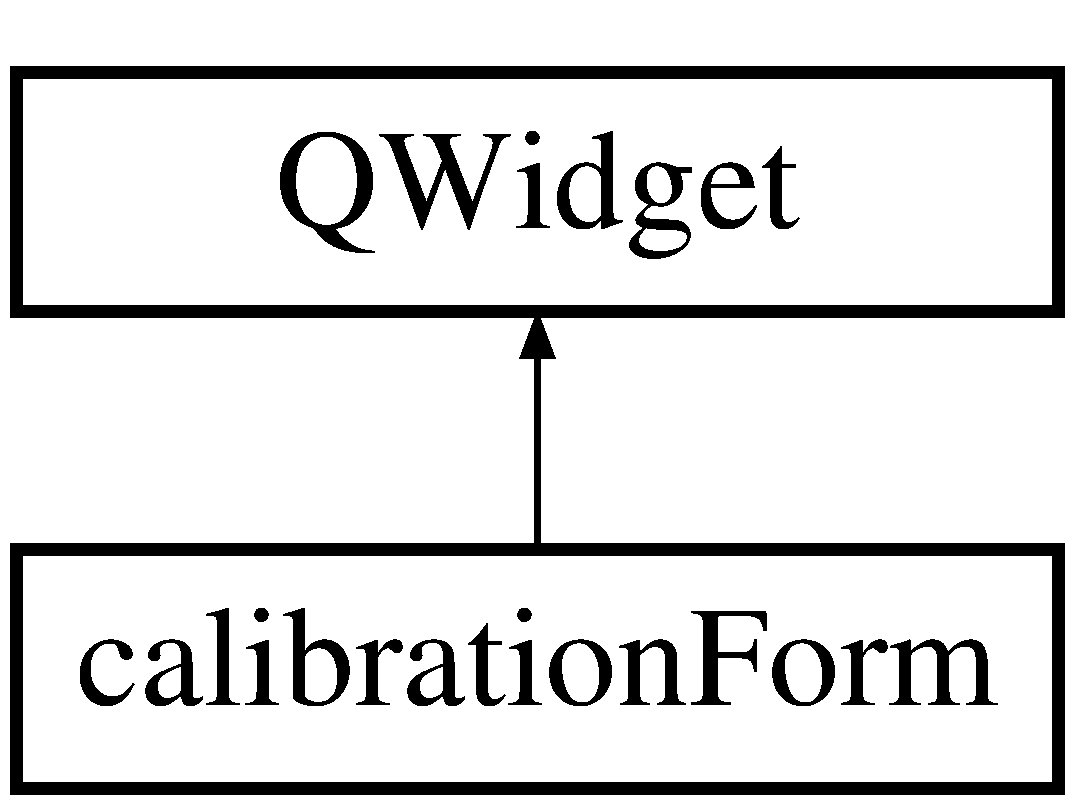
\includegraphics[height=2.000000cm]{classcalibration_form}
\end{center}
\end{figure}
\subsection*{Signals}
\begin{DoxyCompactItemize}
\item 
\hypertarget{classcalibration_form_a4b69dd9a448eb4ae87cab5d2cfcf120b}{}void {\bfseries closed} (void)\label{classcalibration_form_a4b69dd9a448eb4ae87cab5d2cfcf120b}

\item 
\hypertarget{classcalibration_form_a2efdd56cb4d8f8a5174a1c562fd9c279}{}void {\bfseries request\+Image} (char \hyperlink{classcalibration_form_ae670e129fa413d10ac54ce1d0e06bb4b}{C\+C\+D})\label{classcalibration_form_a2efdd56cb4d8f8a5174a1c562fd9c279}

\end{DoxyCompactItemize}
\subsection*{Public Member Functions}
\begin{DoxyCompactItemize}
\item 
\hypertarget{classcalibration_form_a904475e56443f8002f554b2333224bbb}{}{\bfseries calibration\+Form} (Q\+Widget $\ast$parent=0)\label{classcalibration_form_a904475e56443f8002f554b2333224bbb}

\item 
\hypertarget{classcalibration_form_a70baa4a45e9f1df59e0484918977fef1}{}void {\bfseries reset} ()\label{classcalibration_form_a70baa4a45e9f1df59e0484918977fef1}

\end{DoxyCompactItemize}
\subsection*{Public Attributes}
\begin{DoxyCompactItemize}
\item 
\hypertarget{classcalibration_form_afe63228c0cb2ad7c6bade4f38528dc33}{}\hyperlink{classcamera__calibration}{camera\+\_\+calibration} $\ast$ {\bfseries cc}\label{classcalibration_form_afe63228c0cb2ad7c6bade4f38528dc33}

\end{DoxyCompactItemize}
\subsection*{Private Slots}
\begin{DoxyCompactItemize}
\item 
\hypertarget{classcalibration_form_a41bb50ba937dcc523fdef9c5a178728a}{}void {\bfseries on\+\_\+push\+Button\+\_\+3\+\_\+clicked} ()\label{classcalibration_form_a41bb50ba937dcc523fdef9c5a178728a}

\item 
\hypertarget{classcalibration_form_a16256ba3d98cc18d56f25be0391a371e}{}void {\bfseries on\+\_\+push\+Button\+\_\+calibration\+\_\+clicked} ()\label{classcalibration_form_a16256ba3d98cc18d56f25be0391a371e}

\item 
\hypertarget{classcalibration_form_aac07475302f18cd24400dbd6039296ff}{}void {\bfseries mouse\+Release\+Event} (Q\+Mouse\+Event $\ast$)\label{classcalibration_form_aac07475302f18cd24400dbd6039296ff}

\item 
\hypertarget{classcalibration_form_aa86ed00af593676a7c0f172967e330aa}{}void {\bfseries key\+Release\+Event} (Q\+Key\+Event $\ast$event)\label{classcalibration_form_aa86ed00af593676a7c0f172967e330aa}

\item 
void \hyperlink{classcalibration_form_a9682501d6acfcbbcfc52eaac626a2c10}{save\+Image} (cv\+::\+Mat $\ast$img)
\begin{DoxyCompactList}\small\item\em save\+Image is related to \hyperlink{}{Main\+Window\+::send\+Image}\end{DoxyCompactList}\item 
void \hyperlink{classcalibration_form_af82645151b4b3c682996b25ba498581b}{save\+Images} (cv\+::\+Mat $\ast$img\+\_\+\+L, cv\+::\+Mat $\ast$img\+\_\+\+R)
\begin{DoxyCompactList}\small\item\em save\+Images is related to \hyperlink{}{Main\+Window\+::send\+Images}\end{DoxyCompactList}\item 
\hypertarget{classcalibration_form_a46bd3268aef5d6d736732546f22f0ea4}{}void {\bfseries on\+\_\+check\+Box\+\_\+\+Save\+Both\+\_\+clicked} (bool checked)\label{classcalibration_form_a46bd3268aef5d6d736732546f22f0ea4}

\item 
void \hyperlink{classcalibration_form_a1b1f997c7f6d4a592b05e74f53e5b1a8}{get\+Basic\+Info} (int focal\+\_\+length, double base\+\_\+line)
\begin{DoxyCompactList}\small\item\em get\+Basic\+Info to acquire camera\textquotesingle{}s basic info. (related to \hyperlink{}{Main\+Window\+::send\+Basic\+Info)}\end{DoxyCompactList}\item 
\hypertarget{classcalibration_form_a1774fe86a4c7d6d93a4cddefa213a895}{}void {\bfseries on\+\_\+push\+Button\+\_\+corner\+\_\+intrinsic\+\_\+clicked} ()\label{classcalibration_form_a1774fe86a4c7d6d93a4cddefa213a895}

\item 
\hypertarget{classcalibration_form_aebd11d316b6b138ae5685e9047aec962}{}void {\bfseries close\+Event} (Q\+Close\+Event $\ast$)\label{classcalibration_form_aebd11d316b6b138ae5685e9047aec962}

\end{DoxyCompactItemize}
\subsection*{Private Member Functions}
\begin{DoxyCompactItemize}
\item 
\hypertarget{classcalibration_form_aab14476d02bc9543366f4672734c2f7e}{}void {\bfseries load\+Files} (Q\+String folder, std\+::vector$<$ std\+::string $>$ files\mbox{[}$\,$\mbox{]})\label{classcalibration_form_aab14476d02bc9543366f4672734c2f7e}

\item 
\hypertarget{classcalibration_form_a7c5a1fcb7443d7cf31e60c698c328c2e}{}void {\bfseries next\+Cam} ()\label{classcalibration_form_a7c5a1fcb7443d7cf31e60c698c328c2e}

\item 
\hypertarget{classcalibration_form_a73fd9e30a9926512d208e421e30c1045}{}void {\bfseries prev\+Cam} ()\label{classcalibration_form_a73fd9e30a9926512d208e421e30c1045}

\end{DoxyCompactItemize}
\subsection*{Private Attributes}
\begin{DoxyCompactItemize}
\item 
\hypertarget{classcalibration_form_aa6eca629addd8a66ddadc7c23037c120}{}\hyperlink{class_ui_1_1calibration_form}{Ui\+::calibration\+Form} $\ast$ {\bfseries ui}\label{classcalibration_form_aa6eca629addd8a66ddadc7c23037c120}

\item 
\hypertarget{classcalibration_form_ae670e129fa413d10ac54ce1d0e06bb4b}{}char \hyperlink{classcalibration_form_ae670e129fa413d10ac54ce1d0e06bb4b}{C\+C\+D}\label{classcalibration_form_ae670e129fa413d10ac54ce1d0e06bb4b}

\begin{DoxyCompactList}\small\item\em processing C\+C\+D\+: R, L and B. \end{DoxyCompactList}\item 
\hypertarget{classcalibration_form_a9945bc13e7ac54f1d72913876db9cc68}{}char {\bfseries C\+C\+D\+\_\+temp}\label{classcalibration_form_a9945bc13e7ac54f1d72913876db9cc68}

\item 
\hypertarget{classcalibration_form_aabfdd8bde101d1a8bbbc7ee7dfd1c4fd}{}int {\bfseries focal\+\_\+length}\label{classcalibration_form_aabfdd8bde101d1a8bbbc7ee7dfd1c4fd}

\item 
\hypertarget{classcalibration_form_ae3a28bb4bf40337f17129c9e55ac6599}{}double {\bfseries base\+\_\+line}\label{classcalibration_form_ae3a28bb4bf40337f17129c9e55ac6599}

\item 
\hypertarget{classcalibration_form_a98cfb541b6ee63e0bbe16559a15a30e5}{}Q\+Dir {\bfseries image\+\_\+save\+\_\+path}\label{classcalibration_form_a98cfb541b6ee63e0bbe16559a15a30e5}

\item 
\hypertarget{classcalibration_form_a9d6f8bf6a1da0f56bb016f8601b90202}{}Q\+String {\bfseries image\+\_\+save\+\_\+folder}\label{classcalibration_form_a9d6f8bf6a1da0f56bb016f8601b90202}

\item 
\hypertarget{classcalibration_form_a7a98deafc43136f209674303c25100d4}{}Q\+Date\+Time {\bfseries t\+\_\+now}\label{classcalibration_form_a7a98deafc43136f209674303c25100d4}

\item 
\hypertarget{classcalibration_form_ae18c36e51f1c1463e7d41d27831574b8}{}Q\+String {\bfseries t\+\_\+now\+\_\+string}\label{classcalibration_form_ae18c36e51f1c1463e7d41d27831574b8}

\item 
\hypertarget{classcalibration_form_af6078e1bb25e113a7240246578da0022}{}Q\+String {\bfseries file\+\_\+save\+\_\+\+L}\label{classcalibration_form_af6078e1bb25e113a7240246578da0022}

\item 
\hypertarget{classcalibration_form_ad64208e0e84eb05552e5a84296079335}{}Q\+String {\bfseries file\+\_\+save\+\_\+\+R}\label{classcalibration_form_ad64208e0e84eb05552e5a84296079335}

\item 
\hypertarget{classcalibration_form_a78e3b5938f7be0721d8e469b70f3d23b}{}const std\+::string {\bfseries image\+\_\+name\+\_\+\+R} = \char`\"{}Right image\char`\"{}\label{classcalibration_form_a78e3b5938f7be0721d8e469b70f3d23b}

\item 
\hypertarget{classcalibration_form_aaa79b8cc38513f92d244ce1b95556992}{}const std\+::string {\bfseries image\+\_\+name\+\_\+\+L} = \char`\"{}Left image\char`\"{}\label{classcalibration_form_aaa79b8cc38513f92d244ce1b95556992}

\item 
\hypertarget{classcalibration_form_a31551e795742cf5228321c7647fa8ac6}{}cv\+::\+Mat {\bfseries img\+\_\+s\+\_\+\+L}\label{classcalibration_form_a31551e795742cf5228321c7647fa8ac6}

\item 
\hypertarget{classcalibration_form_a2ac2a809bf4a5042d5c12595bf8d4734}{}cv\+::\+Mat {\bfseries img\+\_\+s\+\_\+\+R}\label{classcalibration_form_a2ac2a809bf4a5042d5c12595bf8d4734}

\item 
\hypertarget{classcalibration_form_a259752c35c95e30153abca9e6ea28399}{}Q\+String\+List {\bfseries images\+\_\+\+L}\label{classcalibration_form_a259752c35c95e30153abca9e6ea28399}

\item 
\hypertarget{classcalibration_form_a749ceac9df13ad56870dfa7afbd907b9}{}Q\+String\+List {\bfseries images\+\_\+\+R}\label{classcalibration_form_a749ceac9df13ad56870dfa7afbd907b9}

\end{DoxyCompactItemize}


\subsection{Detailed Description}
The \hyperlink{classcalibration_form}{calibration\+Form} class is a little widget to do the camera calibration. 

\subsection{Member Function Documentation}
\hypertarget{classcalibration_form_a1b1f997c7f6d4a592b05e74f53e5b1a8}{}\index{calibration\+Form@{calibration\+Form}!get\+Basic\+Info@{get\+Basic\+Info}}
\index{get\+Basic\+Info@{get\+Basic\+Info}!calibration\+Form@{calibration\+Form}}
\subsubsection[{get\+Basic\+Info}]{\setlength{\rightskip}{0pt plus 5cm}void calibration\+Form\+::get\+Basic\+Info (
\begin{DoxyParamCaption}
\item[{int}]{focal\+\_\+length, }
\item[{double}]{base\+\_\+line}
\end{DoxyParamCaption}
)\hspace{0.3cm}{\ttfamily [private]}, {\ttfamily [slot]}}\label{classcalibration_form_a1b1f997c7f6d4a592b05e74f53e5b1a8}


get\+Basic\+Info to acquire camera\textquotesingle{}s basic info. (related to \hyperlink{}{Main\+Window\+::send\+Basic\+Info)}


\begin{DoxyParams}{Parameters}
{\em focal\+\_\+length} & \\
\hline
{\em base\+\_\+line} & \\
\hline
\end{DoxyParams}
\hypertarget{classcalibration_form_a9682501d6acfcbbcfc52eaac626a2c10}{}\index{calibration\+Form@{calibration\+Form}!save\+Image@{save\+Image}}
\index{save\+Image@{save\+Image}!calibration\+Form@{calibration\+Form}}
\subsubsection[{save\+Image}]{\setlength{\rightskip}{0pt plus 5cm}void calibration\+Form\+::save\+Image (
\begin{DoxyParamCaption}
\item[{cv\+::\+Mat $\ast$}]{img}
\end{DoxyParamCaption}
)\hspace{0.3cm}{\ttfamily [private]}, {\ttfamily [slot]}}\label{classcalibration_form_a9682501d6acfcbbcfc52eaac626a2c10}


save\+Image is related to \hyperlink{}{Main\+Window\+::send\+Image}


\begin{DoxyParams}{Parameters}
{\em img} & \\
\hline
\end{DoxyParams}
\hypertarget{classcalibration_form_af82645151b4b3c682996b25ba498581b}{}\index{calibration\+Form@{calibration\+Form}!save\+Images@{save\+Images}}
\index{save\+Images@{save\+Images}!calibration\+Form@{calibration\+Form}}
\subsubsection[{save\+Images}]{\setlength{\rightskip}{0pt plus 5cm}void calibration\+Form\+::save\+Images (
\begin{DoxyParamCaption}
\item[{cv\+::\+Mat $\ast$}]{img\+\_\+\+L, }
\item[{cv\+::\+Mat $\ast$}]{img\+\_\+\+R}
\end{DoxyParamCaption}
)\hspace{0.3cm}{\ttfamily [private]}, {\ttfamily [slot]}}\label{classcalibration_form_af82645151b4b3c682996b25ba498581b}


save\+Images is related to \hyperlink{}{Main\+Window\+::send\+Images}


\begin{DoxyParams}{Parameters}
{\em img\+\_\+\+L} & \\
\hline
{\em img\+\_\+\+R} & \\
\hline
\end{DoxyParams}


The documentation for this class was generated from the following files\+:\begin{DoxyCompactItemize}
\item 
D\+:/\+Qt\+Program/\+Qt5/\+Fusion/calibrationform.\+h\item 
D\+:/\+Qt\+Program/\+Qt5/\+Fusion/calibrationform.\+cpp\end{DoxyCompactItemize}

\hypertarget{class_ui_1_1calibration_form}{}\section{Ui\+:\+:calibration\+Form Class Reference}
\label{class_ui_1_1calibration_form}\index{Ui\+::calibration\+Form@{Ui\+::calibration\+Form}}
Inheritance diagram for Ui\+:\+:calibration\+Form\+:\begin{figure}[H]
\begin{center}
\leavevmode
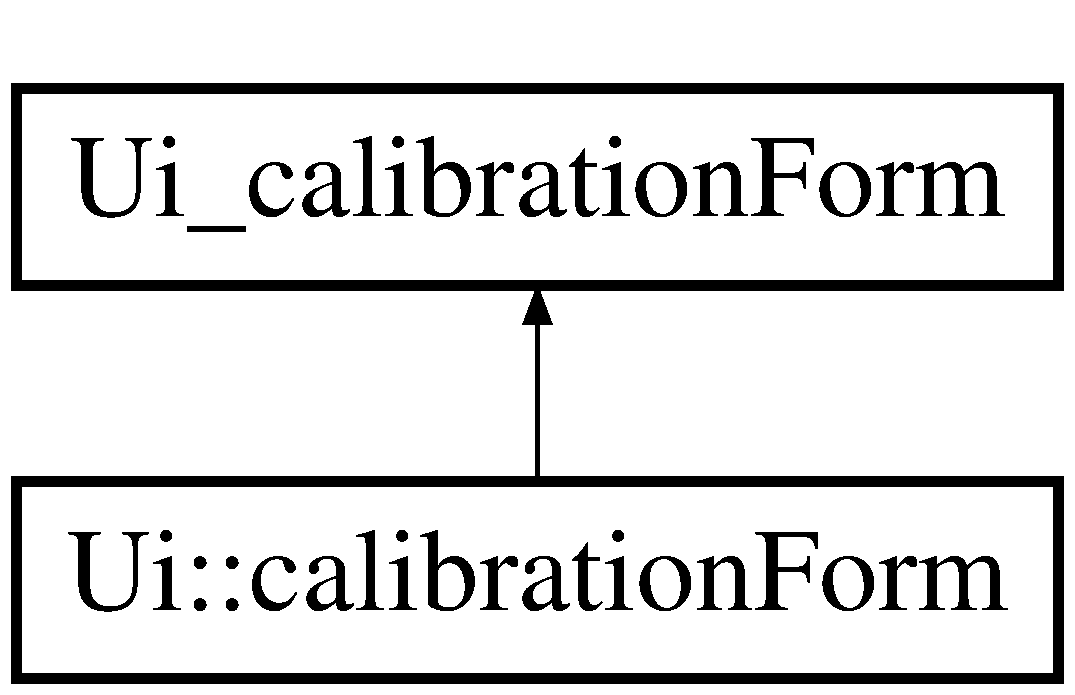
\includegraphics[height=2.000000cm]{class_ui_1_1calibration_form}
\end{center}
\end{figure}
\subsection*{Additional Inherited Members}


The documentation for this class was generated from the following file\+:\begin{DoxyCompactItemize}
\item 
D\+:/\+Qt\+Program/\+Qt5/\+Fusion/ui\+\_\+calibrationform.\+h\end{DoxyCompactItemize}

\hypertarget{classcamera__calibration}{}\section{camera\+\_\+calibration Class Reference}
\label{classcamera__calibration}\index{camera\+\_\+calibration@{camera\+\_\+calibration}}
\subsection*{Signals}
\begin{DoxyCompactItemize}
\item 
\hypertarget{classcamera__calibration_afdb838ba266a33ab8793fa473dfd5de4}{}void {\bfseries save\+Image} ()\label{classcamera__calibration_afdb838ba266a33ab8793fa473dfd5de4}

\end{DoxyCompactItemize}
\subsection*{Public Member Functions}
\begin{DoxyCompactItemize}
\item 
\hypertarget{classcamera__calibration_ae4efd033cabb573f7b29c06cd232c418}{}void {\bfseries Camera\+Calibration} (bool Show\+Pts, cv\+::\+Size Size\+Pattern, cv\+::\+Size2f Size\+Grid, std\+::vector$<$ std\+::string $>$ files)\label{classcamera__calibration_ae4efd033cabb573f7b29c06cd232c418}

\item 
\hypertarget{classcamera__calibration_a6a368ee81537f2affa81827a58bcca39}{}void {\bfseries Find\+Get\+Corner\+Pts} (bool Show\+Pts, std\+::vector$<$ std\+::string $>$ files)\label{classcamera__calibration_a6a368ee81537f2affa81827a58bcca39}

\item 
\hypertarget{classcamera__calibration_a465e652496ec382d61115205b52df4f2}{}void {\bfseries Save\+Intrinsic} (std\+::string \&folder, std\+::string \&filename)\label{classcamera__calibration_a465e652496ec382d61115205b52df4f2}

\item 
\hypertarget{classcamera__calibration_a23d697bb6dff6e69818067a3de785a49}{}void {\bfseries Display\+Undistorted\+Img} (bool Show\+Pts)\label{classcamera__calibration_a23d697bb6dff6e69818067a3de785a49}

\end{DoxyCompactItemize}
\subsection*{Private Member Functions}
\begin{DoxyCompactItemize}
\item 
\hypertarget{classcamera__calibration_a461d87ecc98b610c880b6828ab56c345}{}void {\bfseries Load\+File} (std\+::vector$<$ std\+::string $>$ files)\label{classcamera__calibration_a461d87ecc98b610c880b6828ab56c345}

\item 
\hypertarget{classcamera__calibration_a5ba41d27411f27fd27d55f390eaf4318}{}void {\bfseries Get\+Suppose\+Pts} ()\label{classcamera__calibration_a5ba41d27411f27fd27d55f390eaf4318}

\end{DoxyCompactItemize}
\subsection*{Private Attributes}
\begin{DoxyCompactItemize}
\item 
\hypertarget{classcamera__calibration_a85ae9430f0fc83701195274ecfeabedd}{}std\+::vector$<$ cv\+::\+Mat $>$ {\bfseries img\+Src}\label{classcamera__calibration_a85ae9430f0fc83701195274ecfeabedd}

\item 
\hypertarget{classcamera__calibration_af721b99676dffbd6b76337094abb0364}{}std\+::vector$<$ std\+::vector$<$ cv\+::\+Point3f $>$ $>$ {\bfseries suppose\+Pts}\label{classcamera__calibration_af721b99676dffbd6b76337094abb0364}

\item 
\hypertarget{classcamera__calibration_a861094e4bf699de1bc8e5fb02c6b1e48}{}std\+::vector$<$ std\+::vector$<$ cv\+::\+Point2f $>$ $>$ {\bfseries Pattern\+Pts}\label{classcamera__calibration_a861094e4bf699de1bc8e5fb02c6b1e48}

\item 
\hypertarget{classcamera__calibration_acfe849351fc596d3b7abc05f732d7138}{}cv\+::\+Size \hyperlink{classcamera__calibration_acfe849351fc596d3b7abc05f732d7138}{pattern\+Size}\label{classcamera__calibration_acfe849351fc596d3b7abc05f732d7138}

\begin{DoxyCompactList}\small\item\em Number of corner. \end{DoxyCompactList}\item 
\hypertarget{classcamera__calibration_a93d04e4b624695a6d537efc541dfa901}{}cv\+::\+Size2f \hyperlink{classcamera__calibration_a93d04e4b624695a6d537efc541dfa901}{grid\+Size}\label{classcamera__calibration_a93d04e4b624695a6d537efc541dfa901}

\begin{DoxyCompactList}\small\item\em Size of grid. \end{DoxyCompactList}\item 
\hypertarget{classcamera__calibration_a977e20ebb834c981fe850c0e1bcb7c2e}{}cv\+::\+Mat {\bfseries intrinsic\+Mat}\label{classcamera__calibration_a977e20ebb834c981fe850c0e1bcb7c2e}

\item 
\hypertarget{classcamera__calibration_a9761b3623fc1ad8ca2adf0c65f4a4674}{}cv\+::\+Mat \hyperlink{classcamera__calibration_a9761b3623fc1ad8ca2adf0c65f4a4674}{distortion\+Mat}\label{classcamera__calibration_a9761b3623fc1ad8ca2adf0c65f4a4674}

\begin{DoxyCompactList}\small\item\em Output parameter. \end{DoxyCompactList}\end{DoxyCompactItemize}


The documentation for this class was generated from the following files\+:\begin{DoxyCompactItemize}
\item 
D\+:/\+Qt\+Program/\+Qt5/\+Fusion/camera\+\_\+calibration.\+h\item 
D\+:/\+Qt\+Program/\+Qt5/\+Fusion/camera\+\_\+calibration.\+cpp\end{DoxyCompactItemize}

\hypertarget{structstereo__vision_1_1cam_param}{}\section{stereo\+\_\+vision\+:\+:cam\+Param Struct Reference}
\label{structstereo__vision_1_1cam_param}\index{stereo\+\_\+vision\+::cam\+Param@{stereo\+\_\+vision\+::cam\+Param}}


The \hyperlink{structstereo__vision_1_1cam_param}{cam\+Param} struct for depth estimatiom.  




{\ttfamily \#include $<$stereo\+\_\+vision.\+h$>$}

\subsection*{Public Attributes}
\begin{DoxyCompactItemize}
\item 
\hypertarget{structstereo__vision_1_1cam_param_ab5a239a0dbe3c7079ef18dcb45e1b6ca}{}int {\bfseries port\+\_\+\+L}\label{structstereo__vision_1_1cam_param_ab5a239a0dbe3c7079ef18dcb45e1b6ca}

\item 
\hypertarget{structstereo__vision_1_1cam_param_a8eb191e3eca2630aa82358393083dbe5}{}int {\bfseries port\+\_\+\+R}\label{structstereo__vision_1_1cam_param_a8eb191e3eca2630aa82358393083dbe5}

\item 
\hypertarget{structstereo__vision_1_1cam_param_ab16a090f63e05103059167e0fca24b8a}{}double {\bfseries param\+\_\+r}\label{structstereo__vision_1_1cam_param_ab16a090f63e05103059167e0fca24b8a}

\item 
\hypertarget{structstereo__vision_1_1cam_param_a7bb87f80c0820de75fce40c563103205}{}double {\bfseries focal\+\_\+length}\label{structstereo__vision_1_1cam_param_a7bb87f80c0820de75fce40c563103205}

\item 
\hypertarget{structstereo__vision_1_1cam_param_ac19c2db648f2cb730009f12b145e7aa0}{}int {\bfseries cam\+\_\+focal\+\_\+length}\label{structstereo__vision_1_1cam_param_ac19c2db648f2cb730009f12b145e7aa0}

\item 
\hypertarget{structstereo__vision_1_1cam_param_a4583737f3ea1fde8f47a42e85b96bb98}{}double {\bfseries base\+\_\+line}\label{structstereo__vision_1_1cam_param_a4583737f3ea1fde8f47a42e85b96bb98}

\item 
\hypertarget{structstereo__vision_1_1cam_param_ad7f49fa94e95033ca85828fc788ba7f1}{}double {\bfseries rig\+\_\+height}\label{structstereo__vision_1_1cam_param_ad7f49fa94e95033ca85828fc788ba7f1}

\end{DoxyCompactItemize}


\subsection{Detailed Description}
The \hyperlink{structstereo__vision_1_1cam_param}{cam\+Param} struct for depth estimatiom. 

The documentation for this struct was generated from the following file\+:\begin{DoxyCompactItemize}
\item 
D\+:/\+Qt\+Program/\+Qt5/\+Fusion/stereo\+\_\+vision.\+h\end{DoxyCompactItemize}

\hypertarget{struct_radar_controller_1_1_e_s_r___s_t_a_t}{}\section{Radar\+Controller\+:\+:E\+S\+R\+\_\+\+S\+T\+A\+T Struct Reference}
\label{struct_radar_controller_1_1_e_s_r___s_t_a_t}\index{Radar\+Controller\+::\+E\+S\+R\+\_\+\+S\+T\+A\+T@{Radar\+Controller\+::\+E\+S\+R\+\_\+\+S\+T\+A\+T}}
\subsection*{Classes}
\begin{DoxyCompactItemize}
\item 
struct \hyperlink{struct_radar_controller_1_1_e_s_r___s_t_a_t_1_1_b_r_i_d_g_e___o_b_j_e_c_t}{B\+R\+I\+D\+G\+E\+\_\+\+O\+B\+J\+E\+C\+T}
\item 
struct \hyperlink{struct_radar_controller_1_1_e_s_r___s_t_a_t_1_1_g_r_o_u_p_i_n_g___c_h_a_n_g_e_d}{G\+R\+O\+U\+P\+I\+N\+G\+\_\+\+C\+H\+A\+N\+G\+E\+D}
\item 
struct \hyperlink{struct_radar_controller_1_1_e_s_r___s_t_a_t_1_1_m_e_d___r_a_n_g_e___m_o_d_e}{M\+E\+D\+\_\+\+R\+A\+N\+G\+E\+\_\+\+M\+O\+D\+E}
\item 
struct \hyperlink{struct_radar_controller_1_1_e_s_r___s_t_a_t_1_1_o_n_c_o_m_i_n_g}{O\+N\+C\+O\+M\+I\+N\+G}
\item 
struct \hyperlink{struct_radar_controller_1_1_e_s_r___s_t_a_t_1_1_s_t_a_t_u_s}{S\+T\+A\+T\+U\+S}
\end{DoxyCompactItemize}


The documentation for this struct was generated from the following file\+:\begin{DoxyCompactItemize}
\item 
D\+:/\+Qt\+Program/\+Qt5/\+Fusion/radarcontroller.\+h\end{DoxyCompactItemize}

\hypertarget{struct_radar_controller_1_1_e_s_r___s_t_a_t_1_1_g_r_o_u_p_i_n_g___c_h_a_n_g_e_d}{}\section{Radar\+Controller\+:\+:E\+S\+R\+\_\+\+S\+T\+A\+T\+:\+:G\+R\+O\+U\+P\+I\+N\+G\+\_\+\+C\+H\+A\+N\+G\+E\+D Struct Reference}
\label{struct_radar_controller_1_1_e_s_r___s_t_a_t_1_1_g_r_o_u_p_i_n_g___c_h_a_n_g_e_d}\index{Radar\+Controller\+::\+E\+S\+R\+\_\+\+S\+T\+A\+T\+::\+G\+R\+O\+U\+P\+I\+N\+G\+\_\+\+C\+H\+A\+N\+G\+E\+D@{Radar\+Controller\+::\+E\+S\+R\+\_\+\+S\+T\+A\+T\+::\+G\+R\+O\+U\+P\+I\+N\+G\+\_\+\+C\+H\+A\+N\+G\+E\+D}}
\subsection*{Public Types}
\begin{DoxyCompactItemize}
\item 
\hypertarget{struct_radar_controller_1_1_e_s_r___s_t_a_t_1_1_g_r_o_u_p_i_n_g___c_h_a_n_g_e_d_ad49222ada2e1b946f1c7a5c01a9f3af7}{}enum \{ {\bfseries N\+O} = false, 
{\bfseries Y\+E\+S} = true
 \}\label{struct_radar_controller_1_1_e_s_r___s_t_a_t_1_1_g_r_o_u_p_i_n_g___c_h_a_n_g_e_d_ad49222ada2e1b946f1c7a5c01a9f3af7}

\end{DoxyCompactItemize}


The documentation for this struct was generated from the following file\+:\begin{DoxyCompactItemize}
\item 
D\+:/\+Qt\+Program/\+Qt5/\+Fusion/radarcontroller.\+h\end{DoxyCompactItemize}

\hypertarget{classlrf__controller}{}\section{lrf\+\_\+controller Class Reference}
\label{classlrf__controller}\index{lrf\+\_\+controller@{lrf\+\_\+controller}}


The \hyperlink{classlrf__controller}{lrf\+\_\+controller} class is Laser Range Finder Controller.  




{\ttfamily \#include $<$lrf\+\_\+controller.\+h$>$}

Inheritance diagram for lrf\+\_\+controller\+:\begin{figure}[H]
\begin{center}
\leavevmode
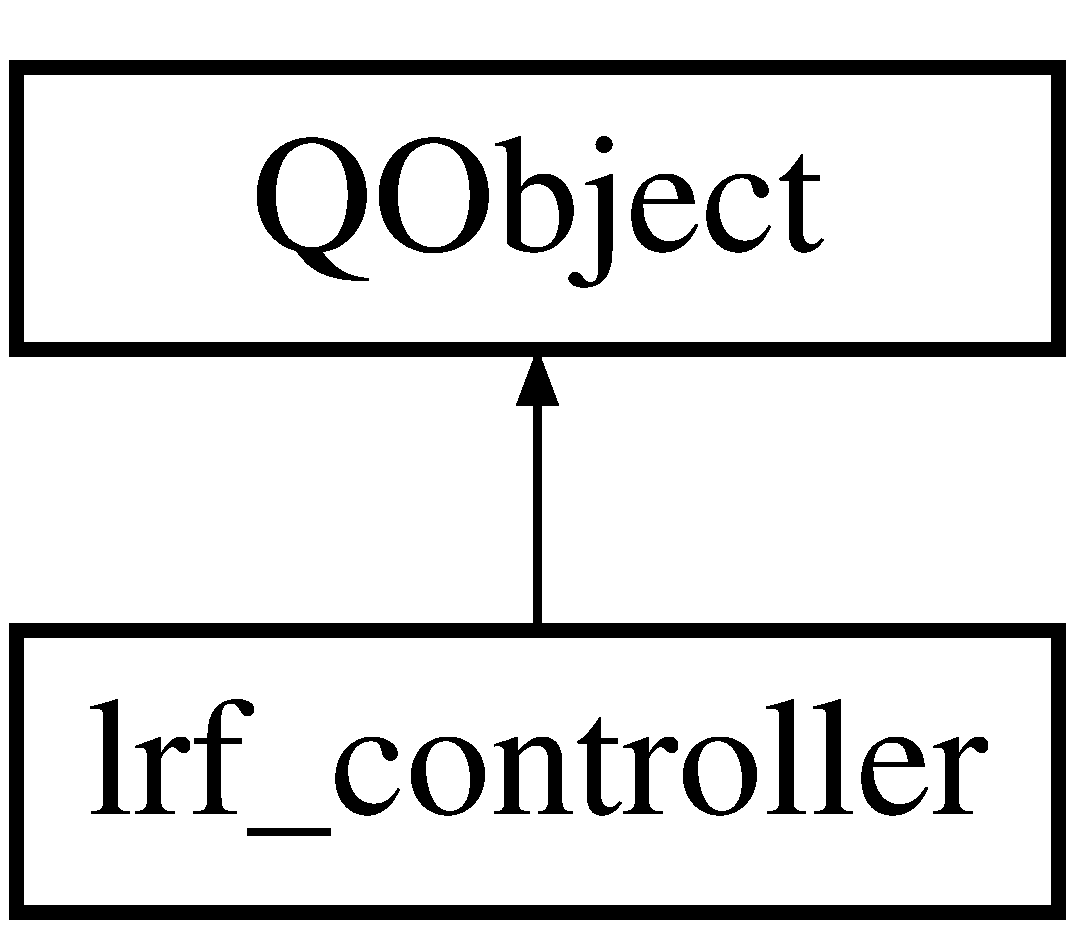
\includegraphics[height=2.000000cm]{classlrf__controller}
\end{center}
\end{figure}
\subsection*{Signals}
\begin{DoxyCompactItemize}
\item 
\hypertarget{classlrf__controller_ae812bd6df2878aca8f1a07fac416992f}{}void {\bfseries update\+G\+U\+I} (double $\ast$data, cv\+::\+Mat $\ast$display\+\_\+lrf)\label{classlrf__controller_ae812bd6df2878aca8f1a07fac416992f}

\end{DoxyCompactItemize}
\subsection*{Public Member Functions}
\begin{DoxyCompactItemize}
\item 
bool \hyperlink{classlrf__controller_a1e0539314437996eb9b832f24385eb16}{open} (Q\+String com\+Port\+In, int baud\+Rate\+In)
\begin{DoxyCompactList}\small\item\em open the serial port connection between P\+C and device \end{DoxyCompactList}\item 
bool \hyperlink{classlrf__controller_a0f807cf3d603af8445dd0db51bceae88}{is\+Open} ()
\begin{DoxyCompactList}\small\item\em is\+Open check if the port is connected \end{DoxyCompactList}\item 
\hypertarget{classlrf__controller_a57bc0e14a2b92e15b45461567346a940}{}void \hyperlink{classlrf__controller_a57bc0e14a2b92e15b45461567346a940}{reset} ()\label{classlrf__controller_a57bc0e14a2b92e15b45461567346a940}

\begin{DoxyCompactList}\small\item\em reset lrf data \end{DoxyCompactList}\item 
\hypertarget{classlrf__controller_af39dce59c5c192b3e2df5a05d5cd03c5}{}bool {\bfseries data\+Exec} ()\label{classlrf__controller_af39dce59c5c192b3e2df5a05d5cd03c5}

\item 
\hypertarget{classlrf__controller_a2540d58a92fd9a26b303336c2ddf2b45}{}bool {\bfseries gui\+Update} ()\label{classlrf__controller_a2540d58a92fd9a26b303336c2ddf2b45}

\item 
\hypertarget{classlrf__controller_adfa7a15f52e0153b88e3b81964189e2f}{}void \hyperlink{classlrf__controller_adfa7a15f52e0153b88e3b81964189e2f}{push\+To\+Buf} ()\label{classlrf__controller_adfa7a15f52e0153b88e3b81964189e2f}

\begin{DoxyCompactList}\small\item\em push\+To\+Buf put acquired info. from device into the \hyperlink{}{buf.}\end{DoxyCompactList}\item 
void \hyperlink{classlrf__controller_a6e01e4ca0763479b6a6b3f37cdef9f46}{request\+Data} (int \hyperlink{classlrf__controller_a805afcd6b3ca2c2b44c4f21b96e33e4c}{mode})
\begin{DoxyCompactList}\small\item\em request\+Data by sending request msg \end{DoxyCompactList}\item 
\hypertarget{classlrf__controller_ad57fba9a6e702535460181a270978843}{}void {\bfseries stop\+Retrieve} ()\label{classlrf__controller_ad57fba9a6e702535460181a270978843}

\item 
bool \hyperlink{classlrf__controller_a7ffb8af0a1f027853b30769eced05c00}{retrieve\+Data} (double $\ast$data)
\begin{DoxyCompactList}\small\item\em retrieve\+Data starts to retrieve the info. from device \end{DoxyCompactList}\item 
\hypertarget{classlrf__controller_af2b8f2aa951973ee7717e55315cd27e3}{}bool {\bfseries close} ()\label{classlrf__controller_af2b8f2aa951973ee7717e55315cd27e3}

\item 
bool \hyperlink{classlrf__controller_a864a9f00f905ed2f24d2dc8b12566e4a}{buf\+Enough\+Set} ()
\begin{DoxyCompactList}\small\item\em buf\+Enough\+Set check if the info. in \hyperlink{classlrf__controller_a5b3e6126b5bf7eddf5b6fa1c1a555cae}{is more than a set for one process }\end{DoxyCompactList}\item 
bool \hyperlink{classlrf__controller_a677dd52d83706b5b4a1a2eae9298c4c7}{buf\+Not\+Full} ()
\begin{DoxyCompactList}\small\item\em buf\+Not\+Full the same as \hyperlink{classlrf__controller_a864a9f00f905ed2f24d2dc8b12566e4a}{buf\+Enough\+Set}\end{DoxyCompactList}\end{DoxyCompactItemize}
\subsection*{Public Attributes}
\begin{DoxyCompactItemize}
\item 
\hypertarget{classlrf__controller_a2de6652ffca4cc196643c9ea0eac2976}{}int {\bfseries time\+\_\+proc}\label{classlrf__controller_a2de6652ffca4cc196643c9ea0eac2976}

\item 
\hypertarget{classlrf__controller_a6d68e5f28c796dcbb4dbcd8b1e8001a5}{}int {\bfseries time\+\_\+proc\+\_\+buf}\label{classlrf__controller_a6d68e5f28c796dcbb4dbcd8b1e8001a5}

\item 
\hypertarget{classlrf__controller_a3e5c7769688db71fd38fe46759b85788}{}int {\bfseries scale\+\_\+ratio} = 2\label{classlrf__controller_a3e5c7769688db71fd38fe46759b85788}

\item 
\hypertarget{classlrf__controller_a525f7428c1314ee5b4ecb57688687aea}{}double $\ast$ {\bfseries lrf\+\_\+data}\label{classlrf__controller_a525f7428c1314ee5b4ecb57688687aea}

\item 
\hypertarget{classlrf__controller_a39858b3a3c07ab8d16d32e70e6ceeb80}{}cv\+::\+Mat {\bfseries display\+\_\+lrf}\label{classlrf__controller_a39858b3a3c07ab8d16d32e70e6ceeb80}

\item 
\hypertarget{classlrf__controller_a493827ca15f31cf435fd72d065e0b9b2}{}cv\+::\+Mat {\bfseries display\+\_\+lrf\+\_\+\+B\+G}\label{classlrf__controller_a493827ca15f31cf435fd72d065e0b9b2}

\end{DoxyCompactItemize}
\subsection*{Private Member Functions}
\begin{DoxyCompactItemize}
\item 
bool \hyperlink{classlrf__controller_a29dcf87fb3936610c10872feb316e787}{send\+Msg} (int \hyperlink{classlrf__controller_a805afcd6b3ca2c2b44c4f21b96e33e4c}{mode})
\begin{DoxyCompactList}\small\item\em send\+Msg to call for the data \end{DoxyCompactList}\item 
\hypertarget{classlrf__controller_aa1221e1b1a79e2246315697ba9bfd85e}{}void \hyperlink{classlrf__controller_aa1221e1b1a79e2246315697ba9bfd85e}{set\+Mode} ()\label{classlrf__controller_aa1221e1b1a79e2246315697ba9bfd85e}

\begin{DoxyCompactList}\small\item\em set\+Mode to choose the mode of retrieving data \end{DoxyCompactList}\item 
bool \hyperlink{classlrf__controller_adc6a847d94992ebd902b757215990a89}{check\+A\+C\+K} (Q\+Byte\+Array \&data, const uchar $\ast$msg\+\_\+ack)
\begin{DoxyCompactList}\small\item\em check\+A\+C\+K \mbox{[}unused\mbox{]} to check the msg \end{DoxyCompactList}\item 
bool \hyperlink{classlrf__controller_acd409f6265a4744a6d462fb903f9ecc8}{check\+Header} (Q\+Byte\+Array \&data, int header\+\_\+type)
\begin{DoxyCompactList}\small\item\em check\+Header to check the msg\textquotesingle{}s header \end{DoxyCompactList}\item 
\hypertarget{classlrf__controller_a1fa9747007d6d262a1caa676c75f4022}{}ushort {\bfseries do\+C\+R\+C} (const Q\+Byte\+Array \&data)\label{classlrf__controller_a1fa9747007d6d262a1caa676c75f4022}

\end{DoxyCompactItemize}
\subsection*{Private Attributes}
\begin{DoxyCompactItemize}
\item 
\hypertarget{classlrf__controller_aa6492c79da222d2be63d04fafdf1803e}{}Q\+Serial\+Port $\ast$ {\bfseries serial}\label{classlrf__controller_aa6492c79da222d2be63d04fafdf1803e}

\item 
\hypertarget{classlrf__controller_a3ebac4db6b1fa224a38b146d39b4424f}{}unsigned char {\bfseries data\+\_\+raw} \mbox{[}L\+E\+N\+G\+T\+H\+\_\+\+R\+A\+W\+\_\+\+D\+A\+T\+A\+\_\+\+O\+N\+C\+E-\/L\+E\+N\+G\+T\+H\+\_\+\+H\+E\+A\+D\+E\+R\+\_\+\+O\+N\+C\+E\mbox{]}\label{classlrf__controller_a3ebac4db6b1fa224a38b146d39b4424f}

\item 
\hypertarget{classlrf__controller_ac3c479a9fa19940bd623b1ae3e2b88e8}{}Q\+Serial\+Port\+::\+Baud\+Rate {\bfseries baud\+Rate}\label{classlrf__controller_ac3c479a9fa19940bd623b1ae3e2b88e8}

\item 
\hypertarget{classlrf__controller_a805afcd6b3ca2c2b44c4f21b96e33e4c}{}int \hyperlink{classlrf__controller_a805afcd6b3ca2c2b44c4f21b96e33e4c}{mode}\label{classlrf__controller_a805afcd6b3ca2c2b44c4f21b96e33e4c}

\begin{DoxyCompactList}\small\item\em current process mode \end{DoxyCompactList}\item 
\hypertarget{classlrf__controller_a9180a22868cb0c7054af1c1abed6ec7b}{}Q\+Time {\bfseries t\+\_\+p}\label{classlrf__controller_a9180a22868cb0c7054af1c1abed6ec7b}

\item 
\hypertarget{classlrf__controller_a9fc493fe1842d5570496df7ebdccdd55}{}Q\+Time \hyperlink{classlrf__controller_a9fc493fe1842d5570496df7ebdccdd55}{t\+\_\+p\+\_\+buf}\label{classlrf__controller_a9fc493fe1842d5570496df7ebdccdd55}

\begin{DoxyCompactList}\small\item\em process time of all exec. \end{DoxyCompactList}\item 
\hypertarget{classlrf__controller_ad293d9d17eba64d16d367eb416e2251b}{}Q\+Time \hyperlink{classlrf__controller_ad293d9d17eba64d16d367eb416e2251b}{t}\label{classlrf__controller_ad293d9d17eba64d16d367eb416e2251b}

\begin{DoxyCompactList}\small\item\em control gui not to update too fast \end{DoxyCompactList}\item 
\hypertarget{classlrf__controller_a018b0f8a2aa7e1c39c0f52d7140187b1}{}int {\bfseries time\+\_\+gap}\label{classlrf__controller_a018b0f8a2aa7e1c39c0f52d7140187b1}

\item 
\hypertarget{classlrf__controller_a5b3e6126b5bf7eddf5b6fa1c1a555cae}{}Q\+Byte\+Array $\ast$ \hyperlink{classlrf__controller_a5b3e6126b5bf7eddf5b6fa1c1a555cae}{buf}\label{classlrf__controller_a5b3e6126b5bf7eddf5b6fa1c1a555cae}

\begin{DoxyCompactList}\small\item\em buffer \end{DoxyCompactList}\item 
\hypertarget{classlrf__controller_ad46f5c4400a4e614a4600da16499af9b}{}int \hyperlink{classlrf__controller_ad46f5c4400a4e614a4600da16499af9b}{dataset\+\_\+size}\label{classlrf__controller_ad46f5c4400a4e614a4600da16499af9b}

\begin{DoxyCompactList}\small\item\em input data size \end{DoxyCompactList}\item 
\hypertarget{classlrf__controller_accef3d18f336db79abaf98765c44b3de}{}int \hyperlink{classlrf__controller_accef3d18f336db79abaf98765c44b3de}{header\+\_\+size}\label{classlrf__controller_accef3d18f336db79abaf98765c44b3de}

\begin{DoxyCompactList}\small\item\em input header size \end{DoxyCompactList}\item 
\hypertarget{classlrf__controller_aac4a934c921fc5f412367c95799db90d}{}qint64 \hyperlink{classlrf__controller_aac4a934c921fc5f412367c95799db90d}{num\+\_\+serial}\label{classlrf__controller_aac4a934c921fc5f412367c95799db90d}

\begin{DoxyCompactList}\small\item\em current info. in the buf \end{DoxyCompactList}\item 
\hypertarget{classlrf__controller_a1caa754bfe92e4b5695d57a07faf9b50}{}qint64 \hyperlink{classlrf__controller_a1caa754bfe92e4b5695d57a07faf9b50}{num\+\_\+lack}\label{classlrf__controller_a1caa754bfe92e4b5695d57a07faf9b50}

\begin{DoxyCompactList}\small\item\em lack how many number to construct one complete data \end{DoxyCompactList}\item 
\hypertarget{classlrf__controller_ade46827d5b722e12f5c930bac0f14578}{}qint64 \hyperlink{classlrf__controller_ade46827d5b722e12f5c930bac0f14578}{num\+\_\+input}\label{classlrf__controller_ade46827d5b722e12f5c930bac0f14578}

\begin{DoxyCompactList}\small\item\em info. amount in the buf \end{DoxyCompactList}\item 
\hypertarget{classlrf__controller_a4656d6056dd73f094a33fecfb820503a}{}Q\+Byte\+Array \hyperlink{classlrf__controller_a4656d6056dd73f094a33fecfb820503a}{data\+Set}\label{classlrf__controller_a4656d6056dd73f094a33fecfb820503a}

\begin{DoxyCompactList}\small\item\em cropped a complete data for use \end{DoxyCompactList}\item 
\hypertarget{classlrf__controller_ab2c456ff3c20ee7664698faf29882e5e}{}bool \hyperlink{classlrf__controller_ab2c456ff3c20ee7664698faf29882e5e}{fg\+\_\+header}\label{classlrf__controller_ab2c456ff3c20ee7664698faf29882e5e}

\begin{DoxyCompactList}\small\item\em check header \end{DoxyCompactList}\end{DoxyCompactItemize}


\subsection{Detailed Description}
The \hyperlink{classlrf__controller}{lrf\+\_\+controller} class is Laser Range Finder Controller. 

\subsection{Member Function Documentation}
\hypertarget{classlrf__controller_a864a9f00f905ed2f24d2dc8b12566e4a}{}\index{lrf\+\_\+controller@{lrf\+\_\+controller}!buf\+Enough\+Set@{buf\+Enough\+Set}}
\index{buf\+Enough\+Set@{buf\+Enough\+Set}!lrf\+\_\+controller@{lrf\+\_\+controller}}
\subsubsection[{buf\+Enough\+Set}]{\setlength{\rightskip}{0pt plus 5cm}bool lrf\+\_\+controller\+::buf\+Enough\+Set (
\begin{DoxyParamCaption}
{}
\end{DoxyParamCaption}
)\hspace{0.3cm}{\ttfamily [inline]}}\label{classlrf__controller_a864a9f00f905ed2f24d2dc8b12566e4a}


buf\+Enough\+Set check if the info. in \hyperlink{classlrf__controller_a5b3e6126b5bf7eddf5b6fa1c1a555cae}{is more than a set for one process }

\begin{DoxyReturn}{Returns}

\end{DoxyReturn}
\hypertarget{classlrf__controller_a677dd52d83706b5b4a1a2eae9298c4c7}{}\index{lrf\+\_\+controller@{lrf\+\_\+controller}!buf\+Not\+Full@{buf\+Not\+Full}}
\index{buf\+Not\+Full@{buf\+Not\+Full}!lrf\+\_\+controller@{lrf\+\_\+controller}}
\subsubsection[{buf\+Not\+Full}]{\setlength{\rightskip}{0pt plus 5cm}bool lrf\+\_\+controller\+::buf\+Not\+Full (
\begin{DoxyParamCaption}
{}
\end{DoxyParamCaption}
)\hspace{0.3cm}{\ttfamily [inline]}}\label{classlrf__controller_a677dd52d83706b5b4a1a2eae9298c4c7}


buf\+Not\+Full the same as \hyperlink{classlrf__controller_a864a9f00f905ed2f24d2dc8b12566e4a}{buf\+Enough\+Set}

\begin{DoxyReturn}{Returns}

\end{DoxyReturn}
\hypertarget{classlrf__controller_adc6a847d94992ebd902b757215990a89}{}\index{lrf\+\_\+controller@{lrf\+\_\+controller}!check\+A\+C\+K@{check\+A\+C\+K}}
\index{check\+A\+C\+K@{check\+A\+C\+K}!lrf\+\_\+controller@{lrf\+\_\+controller}}
\subsubsection[{check\+A\+C\+K}]{\setlength{\rightskip}{0pt plus 5cm}bool lrf\+\_\+controller\+::check\+A\+C\+K (
\begin{DoxyParamCaption}
\item[{Q\+Byte\+Array \&}]{data, }
\item[{const uchar $\ast$}]{msg\+\_\+ack}
\end{DoxyParamCaption}
)\hspace{0.3cm}{\ttfamily [private]}}\label{classlrf__controller_adc6a847d94992ebd902b757215990a89}


check\+A\+C\+K \mbox{[}unused\mbox{]} to check the msg 


\begin{DoxyParams}{Parameters}
{\em data} & \\
\hline
{\em msg\+\_\+ack} & \\
\hline
\end{DoxyParams}
\begin{DoxyReturn}{Returns}

\end{DoxyReturn}
\hypertarget{classlrf__controller_acd409f6265a4744a6d462fb903f9ecc8}{}\index{lrf\+\_\+controller@{lrf\+\_\+controller}!check\+Header@{check\+Header}}
\index{check\+Header@{check\+Header}!lrf\+\_\+controller@{lrf\+\_\+controller}}
\subsubsection[{check\+Header}]{\setlength{\rightskip}{0pt plus 5cm}bool lrf\+\_\+controller\+::check\+Header (
\begin{DoxyParamCaption}
\item[{Q\+Byte\+Array \&}]{data, }
\item[{int}]{header\+\_\+type}
\end{DoxyParamCaption}
)\hspace{0.3cm}{\ttfamily [private]}}\label{classlrf__controller_acd409f6265a4744a6d462fb903f9ecc8}


check\+Header to check the msg\textquotesingle{}s header 


\begin{DoxyParams}{Parameters}
{\em data} & \\
\hline
{\em header\+\_\+type} & \\
\hline
\end{DoxyParams}
\begin{DoxyReturn}{Returns}

\end{DoxyReturn}
\hypertarget{classlrf__controller_a0f807cf3d603af8445dd0db51bceae88}{}\index{lrf\+\_\+controller@{lrf\+\_\+controller}!is\+Open@{is\+Open}}
\index{is\+Open@{is\+Open}!lrf\+\_\+controller@{lrf\+\_\+controller}}
\subsubsection[{is\+Open}]{\setlength{\rightskip}{0pt plus 5cm}bool lrf\+\_\+controller\+::is\+Open (
\begin{DoxyParamCaption}
{}
\end{DoxyParamCaption}
)\hspace{0.3cm}{\ttfamily [inline]}}\label{classlrf__controller_a0f807cf3d603af8445dd0db51bceae88}


is\+Open check if the port is connected 

\begin{DoxyReturn}{Returns}

\end{DoxyReturn}
\hypertarget{classlrf__controller_a1e0539314437996eb9b832f24385eb16}{}\index{lrf\+\_\+controller@{lrf\+\_\+controller}!open@{open}}
\index{open@{open}!lrf\+\_\+controller@{lrf\+\_\+controller}}
\subsubsection[{open}]{\setlength{\rightskip}{0pt plus 5cm}bool lrf\+\_\+controller\+::open (
\begin{DoxyParamCaption}
\item[{Q\+String}]{com\+Port\+In, }
\item[{int}]{baud\+Rate\+In}
\end{DoxyParamCaption}
)}\label{classlrf__controller_a1e0539314437996eb9b832f24385eb16}


open the serial port connection between P\+C and device 


\begin{DoxyParams}{Parameters}
{\em com\+Port\+In} & port number \\
\hline
{\em baud\+Rate\+In} & communication baud rate \\
\hline
\end{DoxyParams}
\begin{DoxyReturn}{Returns}

\end{DoxyReturn}
\hypertarget{classlrf__controller_a6e01e4ca0763479b6a6b3f37cdef9f46}{}\index{lrf\+\_\+controller@{lrf\+\_\+controller}!request\+Data@{request\+Data}}
\index{request\+Data@{request\+Data}!lrf\+\_\+controller@{lrf\+\_\+controller}}
\subsubsection[{request\+Data}]{\setlength{\rightskip}{0pt plus 5cm}void lrf\+\_\+controller\+::request\+Data (
\begin{DoxyParamCaption}
\item[{int}]{mode}
\end{DoxyParamCaption}
)}\label{classlrf__controller_a6e01e4ca0763479b6a6b3f37cdef9f46}


request\+Data by sending request msg 


\begin{DoxyParams}{Parameters}
{\em mode} & once and continuous~\newline
once mode\+: header\+\_\+data pop up~\newline
continuous mode\+: A\+C\+K first and come up w/ header data w/o first uchar 0x06~\newline
S\+O, header in O\+N\+C\+E and C\+O\+N\+T\+I is 7 and 8 respectively. \\
\hline
\end{DoxyParams}
\hypertarget{classlrf__controller_a7ffb8af0a1f027853b30769eced05c00}{}\index{lrf\+\_\+controller@{lrf\+\_\+controller}!retrieve\+Data@{retrieve\+Data}}
\index{retrieve\+Data@{retrieve\+Data}!lrf\+\_\+controller@{lrf\+\_\+controller}}
\subsubsection[{retrieve\+Data}]{\setlength{\rightskip}{0pt plus 5cm}bool lrf\+\_\+controller\+::retrieve\+Data (
\begin{DoxyParamCaption}
\item[{double $\ast$}]{data}
\end{DoxyParamCaption}
)}\label{classlrf__controller_a7ffb8af0a1f027853b30769eced05c00}


retrieve\+Data starts to retrieve the info. from device 


\begin{DoxyParams}{Parameters}
{\em data} & the storage of device\textquotesingle{}s info. \\
\hline
\end{DoxyParams}
\begin{DoxyReturn}{Returns}

\end{DoxyReturn}
\hypertarget{classlrf__controller_a29dcf87fb3936610c10872feb316e787}{}\index{lrf\+\_\+controller@{lrf\+\_\+controller}!send\+Msg@{send\+Msg}}
\index{send\+Msg@{send\+Msg}!lrf\+\_\+controller@{lrf\+\_\+controller}}
\subsubsection[{send\+Msg}]{\setlength{\rightskip}{0pt plus 5cm}bool lrf\+\_\+controller\+::send\+Msg (
\begin{DoxyParamCaption}
\item[{int}]{mode}
\end{DoxyParamCaption}
)\hspace{0.3cm}{\ttfamily [private]}}\label{classlrf__controller_a29dcf87fb3936610c10872feb316e787}


send\+Msg to call for the data 


\begin{DoxyParams}{Parameters}
{\em mode} & \\
\hline
\end{DoxyParams}
\begin{DoxyReturn}{Returns}

\end{DoxyReturn}


The documentation for this class was generated from the following files\+:\begin{DoxyCompactItemize}
\item 
D\+:/\+Qt\+Program/\+Qt5/\+Fusion/lrf\+\_\+controller.\+h\item 
D\+:/\+Qt\+Program/\+Qt5/\+Fusion/lrf\+\_\+controller.\+cpp\end{DoxyCompactItemize}

\hypertarget{class_main_window}{}\section{Main\+Window Class Reference}
\label{class_main_window}\index{Main\+Window@{Main\+Window}}


The \hyperlink{class_main_window}{Main\+Window} class.  




{\ttfamily \#include $<$mainwindow.\+h$>$}

Inheritance diagram for Main\+Window\+:\begin{figure}[H]
\begin{center}
\leavevmode
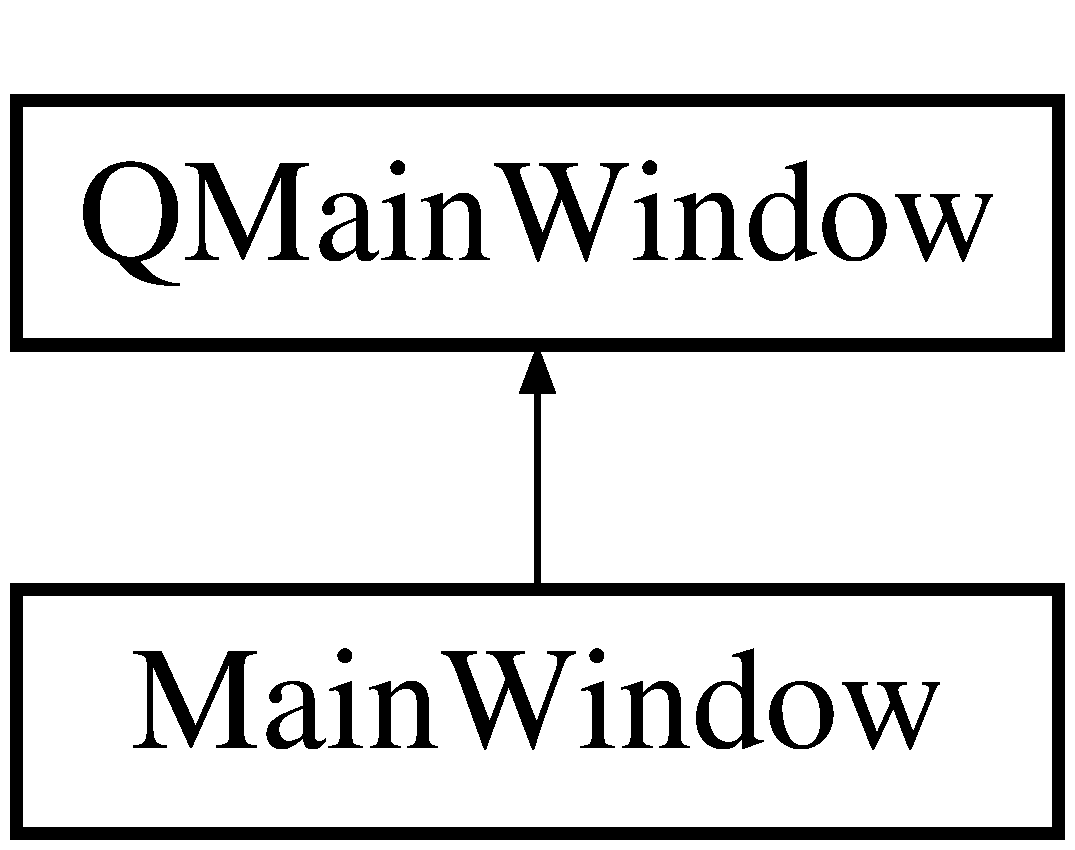
\includegraphics[height=2.000000cm]{class_main_window}
\end{center}
\end{figure}
\subsection*{Signals}
\begin{DoxyCompactItemize}
\item 
\hypertarget{class_main_window_a166aeaf752a430f7468b205c9b514b25}{}void {\bfseries send\+Basic\+Info} (int focal\+\_\+length, double base\+\_\+line)\label{class_main_window_a166aeaf752a430f7468b205c9b514b25}

\item 
\hypertarget{class_main_window_a0f8dabec720e115a310c35407bef31db}{}void {\bfseries send\+Image} (cv\+::\+Mat $\ast$img)\label{class_main_window_a0f8dabec720e115a310c35407bef31db}

\item 
\hypertarget{class_main_window_ada48458b0cdedebe20094d9888e955b0}{}void {\bfseries send\+Images} (cv\+::\+Mat $\ast$img\+\_\+\+L, cv\+::\+Mat $\ast$img\+\_\+\+R)\label{class_main_window_ada48458b0cdedebe20094d9888e955b0}

\end{DoxyCompactItemize}
\subsection*{Public Member Functions}
\begin{DoxyCompactItemize}
\item 
\hypertarget{class_main_window_a8b244be8b7b7db1b08de2a2acb9409db}{}{\bfseries Main\+Window} (Q\+Widget $\ast$parent=0)\label{class_main_window_a8b244be8b7b7db1b08de2a2acb9409db}

\end{DoxyCompactItemize}
\subsection*{Private Slots}
\begin{DoxyCompactItemize}
\item 
\hypertarget{class_main_window_a51927fde27346887663f8b1c8f83f5ab}{}void {\bfseries on\+\_\+push\+Button\+\_\+start\+\_\+all\+\_\+clicked} ()\label{class_main_window_a51927fde27346887663f8b1c8f83f5ab}

\item 
\hypertarget{class_main_window_a6b690c4d5c729e417ccc16fd730c452c}{}void {\bfseries on\+\_\+push\+Button\+\_\+stop\+\_\+all\+\_\+clicked} ()\label{class_main_window_a6b690c4d5c729e417ccc16fd730c452c}

\item 
\hypertarget{class_main_window_afbe2ceefce1abb0886094990582b988d}{}void {\bfseries on\+\_\+action\+Shortcut\+\_\+triggered} ()\label{class_main_window_afbe2ceefce1abb0886094990582b988d}

\item 
\hypertarget{class_main_window_a253e4560fc116df7949f20992ed0b734}{}void {\bfseries on\+\_\+action\+Author\+\_\+triggered} ()\label{class_main_window_a253e4560fc116df7949f20992ed0b734}

\item 
void \hyperlink{class_main_window_ae81612c12f590a4bc599332e71f52afc}{mouse\+X\+Y} (int x, int y)
\begin{DoxyCompactList}\small\item\em mouse\+X\+Y is to acuire mouse info. connect w/ the label \end{DoxyCompactList}\item 
void \hyperlink{class_main_window_ad6984d1fa1808b8406cbc30c5df26415}{wheel\+Event} (Q\+Wheel\+Event $\ast$ev)
\begin{DoxyCompactList}\small\item\em wheel\+Event is to acuire the wheel event \end{DoxyCompactList}\item 
\hypertarget{class_main_window_aa6d34cf000b53f621ecbee7bb9b4d5d2}{}void {\bfseries key\+Press\+Event} (Q\+Key\+Event $\ast$ev)\label{class_main_window_aa6d34cf000b53f621ecbee7bb9b4d5d2}

\item 
\hypertarget{class_main_window_a40746f5a56cdde34925b396fd8d67b89}{}void {\bfseries on\+\_\+push\+Button\+\_\+lrf\+\_\+open\+\_\+clicked} ()\label{class_main_window_a40746f5a56cdde34925b396fd8d67b89}

\item 
\hypertarget{class_main_window_ac0f5decb67a200a028da33ea7e22323b}{}void {\bfseries lrf\+Display} (double $\ast$lrf\+\_\+data, cv\+::\+Mat $\ast$\hyperlink{class_main_window_a526afc9bb96e26cccbc074ed30c7c386}{display\+\_\+lrf})\label{class_main_window_ac0f5decb67a200a028da33ea7e22323b}

\item 
\hypertarget{class_main_window_abe620c8361efe98ca34a574c1e3bb23a}{}void {\bfseries on\+\_\+push\+Button\+\_\+lrf\+\_\+request\+\_\+clicked} ()\label{class_main_window_abe620c8361efe98ca34a574c1e3bb23a}

\item 
\hypertarget{class_main_window_a0eeb2e8245dab36d1555374f38f90b0e}{}void {\bfseries on\+\_\+push\+Button\+\_\+lrf\+\_\+retrieve\+\_\+clicked} ()\label{class_main_window_a0eeb2e8245dab36d1555374f38f90b0e}

\item 
\hypertarget{class_main_window_a978525da6f1ffd7d028e614cb54a28f8}{}void {\bfseries on\+\_\+push\+Button\+\_\+lrf\+\_\+stop\+\_\+clicked} ()\label{class_main_window_a978525da6f1ffd7d028e614cb54a28f8}

\item 
\hypertarget{class_main_window_ad69d20e6e49f01f56636ac2f23420120}{}void {\bfseries on\+\_\+push\+Button\+\_\+lrf\+\_\+request\+\_\+\+O\+N\+C\+E\+\_\+clicked} ()\label{class_main_window_ad69d20e6e49f01f56636ac2f23420120}

\item 
\hypertarget{class_main_window_ad64bbcfe72cae71d26d03ccd11d56787}{}void {\bfseries on\+\_\+push\+Button\+\_\+lrf\+\_\+record\+\_\+data\+\_\+clicked} ()\label{class_main_window_ad64bbcfe72cae71d26d03ccd11d56787}

\item 
\hypertarget{class_main_window_a22c8c805835969894435ddd7e56db854}{}void {\bfseries on\+\_\+push\+Button\+\_\+lrf\+\_\+record\+\_\+stop\+\_\+clicked} ()\label{class_main_window_a22c8c805835969894435ddd7e56db854}

\item 
\hypertarget{class_main_window_a32c1032023f0ceebb217ca49ae94783b}{}void {\bfseries on\+\_\+push\+Button\+\_\+lrf\+\_\+read\+\_\+range\+\_\+clicked} ()\label{class_main_window_a32c1032023f0ceebb217ca49ae94783b}

\item 
\hypertarget{class_main_window_ad9fb96fc74a34efed0f99274c02fc7d9}{}void {\bfseries on\+\_\+push\+Button\+\_\+cam\+\_\+open\+\_\+clicked} ()\label{class_main_window_ad9fb96fc74a34efed0f99274c02fc7d9}

\item 
\hypertarget{class_main_window_a9dba31f02f55c580aa005163c0ad55bb}{}void {\bfseries on\+\_\+push\+Button\+\_\+cam\+\_\+stop\+\_\+clicked} ()\label{class_main_window_a9dba31f02f55c580aa005163c0ad55bb}

\item 
\hypertarget{class_main_window_a2c809869d0bfe5017feb9d3af9d04032}{}void {\bfseries on\+\_\+push\+Button\+\_\+cam\+\_\+step\+\_\+clicked} ()\label{class_main_window_a2c809869d0bfe5017feb9d3af9d04032}

\item 
\hypertarget{class_main_window_a38e6a6d2b814e8547a575729ef91bba1}{}void {\bfseries on\+\_\+push\+Button\+\_\+cam\+\_\+capture\+\_\+clicked} ()\label{class_main_window_a38e6a6d2b814e8547a575729ef91bba1}

\item 
\hypertarget{class_main_window_a64cc3067de847cd79997c8d5bc2f147c}{}void {\bfseries on\+\_\+check\+Box\+\_\+do\+\_\+calibration\+\_\+clicked} (bool checked)\label{class_main_window_a64cc3067de847cd79997c8d5bc2f147c}

\item 
\hypertarget{class_main_window_aa447259fa7c91de734ced19ae24368bc}{}void {\bfseries on\+\_\+check\+Box\+\_\+do\+\_\+depth\+\_\+clicked} (bool checked)\label{class_main_window_aa447259fa7c91de734ced19ae24368bc}

\item 
\hypertarget{class_main_window_ae9bae4b6ce15716892551a698d751128}{}void {\bfseries sv\+Display} (cv\+::\+Mat $\ast$img\+\_\+\+L, cv\+::\+Mat $\ast$img\+\_\+\+R, cv\+::\+Mat $\ast$disp, cv\+::\+Mat $\ast$disp\+\_\+pseudo, cv\+::\+Mat $\ast$topview, cv\+::\+Mat $\ast$img\+\_\+detected, int detected\+\_\+obj, int current\+\_\+frame\+\_\+count)\label{class_main_window_ae9bae4b6ce15716892551a698d751128}

\item 
\hypertarget{class_main_window_a355975f6b124c66571ce71019ed8340c}{}void {\bfseries close\+Form\+Smp} (void)\label{class_main_window_a355975f6b124c66571ce71019ed8340c}

\item 
\hypertarget{class_main_window_a4e8c0c6d5d5cefa708138fdadfcffc5a}{}void {\bfseries on\+\_\+radio\+Button\+\_\+\+B\+M\+\_\+clicked} ()\label{class_main_window_a4e8c0c6d5d5cefa708138fdadfcffc5a}

\item 
\hypertarget{class_main_window_aca90b3e646f2f2175972b86b7f447729}{}void {\bfseries on\+\_\+radio\+Button\+\_\+\+S\+G\+B\+M\+\_\+clicked} ()\label{class_main_window_aca90b3e646f2f2175972b86b7f447729}

\item 
\hypertarget{class_main_window_ad21b3bf3184684c58f48c50e2818e2d2}{}void {\bfseries on\+\_\+line\+Edit\+\_\+sv\+\_\+focal\+\_\+length\+\_\+return\+Pressed} ()\label{class_main_window_ad21b3bf3184684c58f48c50e2818e2d2}

\item 
\hypertarget{class_main_window_aa06fa5822c8b49551444306d38eb7581}{}void {\bfseries on\+\_\+check\+Box\+\_\+sv\+\_\+topview\+\_\+clicked} (bool checked)\label{class_main_window_aa06fa5822c8b49551444306d38eb7581}

\item 
\hypertarget{class_main_window_aa6f408ff31e7af45608a2e8d2e1ff420}{}void {\bfseries on\+\_\+spin\+Box\+\_\+topview\+\_\+r\+\_\+value\+Changed} (int arg1)\label{class_main_window_aa6f408ff31e7af45608a2e8d2e1ff420}

\item 
\hypertarget{class_main_window_a192351847dee86607cb895e960b73abf}{}void {\bfseries on\+\_\+spin\+Box\+\_\+topview\+\_\+c\+\_\+value\+Changed} (int arg1)\label{class_main_window_a192351847dee86607cb895e960b73abf}

\item 
\hypertarget{class_main_window_a3231412e9991f9e2983b8dbbf1eb12a0}{}void {\bfseries on\+\_\+push\+Button\+\_\+stereo\+\_\+match\+\_\+param\+\_\+clicked} ()\label{class_main_window_a3231412e9991f9e2983b8dbbf1eb12a0}

\item 
\hypertarget{class_main_window_a22b957f8849f75f4b8bbc5258395c874}{}void {\bfseries on\+\_\+combo\+Box\+\_\+camera\+\_\+focal\+\_\+length\+\_\+current\+Index\+Changed} (int index)\label{class_main_window_a22b957f8849f75f4b8bbc5258395c874}

\item 
\hypertarget{class_main_window_a49115ba3b5ec385e73ceeebc8091e909}{}void {\bfseries on\+\_\+line\+Edit\+\_\+base\+\_\+line\+\_\+return\+Pressed} ()\label{class_main_window_a49115ba3b5ec385e73ceeebc8091e909}

\item 
\hypertarget{class_main_window_a00b2cebc1a81b57870c2c61b53781d77}{}void {\bfseries on\+\_\+check\+Box\+\_\+pseudo\+\_\+color\+\_\+clicked} (bool checked)\label{class_main_window_a00b2cebc1a81b57870c2c61b53781d77}

\item 
\hypertarget{class_main_window_af81c40636f6d1d6003ab6f7b93040269}{}void {\bfseries on\+\_\+check\+Box\+\_\+topview\+\_\+plot\+\_\+points\+\_\+clicked} (bool checked)\label{class_main_window_af81c40636f6d1d6003ab6f7b93040269}

\item 
\hypertarget{class_main_window_a0aae20901f69daabe680857a395110e0}{}void {\bfseries on\+\_\+check\+Box\+\_\+sv\+\_\+reproject\+\_\+clicked} (bool checked)\label{class_main_window_a0aae20901f69daabe680857a395110e0}

\item 
\hypertarget{class_main_window_a2c53b4338460d00fc3697cb8efed06d7}{}void {\bfseries on\+\_\+push\+Button\+\_\+sv\+\_\+record\+\_\+data\+\_\+clicked} ()\label{class_main_window_a2c53b4338460d00fc3697cb8efed06d7}

\item 
\hypertarget{class_main_window_a687c29593e3b6a93edf08d5d77291968}{}void {\bfseries on\+\_\+push\+Button\+\_\+sv\+\_\+read\+\_\+images\+\_\+clicked} ()\label{class_main_window_a687c29593e3b6a93edf08d5d77291968}

\item 
\hypertarget{class_main_window_a64d21d3127c3d0a9f67f393cd6e31c1c}{}void {\bfseries on\+\_\+push\+Button\+\_\+sv\+\_\+read\+\_\+disp\+\_\+clicked} ()\label{class_main_window_a64d21d3127c3d0a9f67f393cd6e31c1c}

\item 
\hypertarget{class_main_window_a7ee33b0bedeec00f1d770c15e3c5fca1}{}void {\bfseries on\+\_\+push\+Button\+\_\+camera\+\_\+calibration\+\_\+clicked} ()\label{class_main_window_a7ee33b0bedeec00f1d770c15e3c5fca1}

\item 
\hypertarget{class_main_window_a38edb88d43e844aca9d2e762c8706565}{}void {\bfseries close\+Event} (Q\+Close\+Event $\ast$)\label{class_main_window_a38edb88d43e844aca9d2e762c8706565}

\item 
\hypertarget{class_main_window_a968ecf19dc77ae5349a8939e57d53158}{}void {\bfseries request\+Image} (char C\+C\+D)\label{class_main_window_a968ecf19dc77ae5349a8939e57d53158}

\item 
\hypertarget{class_main_window_aac73d81c8d0722a100c6869bfc89a860}{}void {\bfseries close\+Form\+Calib} (void)\label{class_main_window_aac73d81c8d0722a100c6869bfc89a860}

\item 
\hypertarget{class_main_window_ab10389a1cab0e600c8e161a647b4b29d}{}void {\bfseries radar\+Display} (int detected\+\_\+obj, cv\+::\+Mat $\ast$img, cv\+::\+Mat $\ast$topview)\label{class_main_window_ab10389a1cab0e600c8e161a647b4b29d}

\item 
\hypertarget{class_main_window_ac9ea72cd1b942a15a163cb308e6fb656}{}void {\bfseries on\+\_\+push\+Button\+\_\+radar\+\_\+write\+\_\+clicked} ()\label{class_main_window_ac9ea72cd1b942a15a163cb308e6fb656}

\item 
\hypertarget{class_main_window_a76a71322a2f8bc6f01f7a707cc73093e}{}void {\bfseries on\+\_\+push\+Button\+\_\+radar\+\_\+bus\+\_\+on\+\_\+clicked} ()\label{class_main_window_a76a71322a2f8bc6f01f7a707cc73093e}

\item 
\hypertarget{class_main_window_a3a75e1394b03fc2fa74f4f2fbe2f88d9}{}void {\bfseries on\+\_\+push\+Button\+\_\+radar\+\_\+bus\+\_\+off\+\_\+clicked} ()\label{class_main_window_a3a75e1394b03fc2fa74f4f2fbe2f88d9}

\item 
\hypertarget{class_main_window_a5b0bba61eff7a7257c03c85a42afb70f}{}void {\bfseries on\+\_\+push\+Button\+\_\+radar\+\_\+open\+\_\+clicked} ()\label{class_main_window_a5b0bba61eff7a7257c03c85a42afb70f}

\item 
\hypertarget{class_main_window_a13a9eb8072e61993c1ee52d1dcf6843c}{}void {\bfseries on\+\_\+check\+Box\+\_\+radar\+\_\+topview\+\_\+clicked} (bool checked)\label{class_main_window_a13a9eb8072e61993c1ee52d1dcf6843c}

\item 
\hypertarget{class_main_window_ade269ccff5b9b26d487423d31ec19adf}{}void {\bfseries on\+\_\+spin\+Box\+\_\+radar\+\_\+topview\+\_\+r\+\_\+value\+Changed} (int arg1)\label{class_main_window_ade269ccff5b9b26d487423d31ec19adf}

\item 
\hypertarget{class_main_window_a8f2714912f4335593fcc6a4cd1999dd9}{}void {\bfseries on\+\_\+spin\+Box\+\_\+radar\+\_\+topview\+\_\+c\+\_\+value\+Changed} (int arg1)\label{class_main_window_a8f2714912f4335593fcc6a4cd1999dd9}

\item 
\hypertarget{class_main_window_a5ae4659c9b00e173fe6214e10c76e925}{}void {\bfseries fused\+Display} (cv\+::\+Mat $\ast$fused\+\_\+topview, cv\+::\+Mat $\ast$img\+\_\+detected\+\_\+display)\label{class_main_window_a5ae4659c9b00e173fe6214e10c76e925}

\item 
\hypertarget{class_main_window_a5363260e5ea8d86839f8ce9bd8f82cf1}{}void {\bfseries on\+\_\+horizontal\+Slider\+\_\+2\+\_\+slider\+Released} ()\label{class_main_window_a5363260e5ea8d86839f8ce9bd8f82cf1}

\item 
\hypertarget{class_main_window_aee38d2cc3c3f234bb29c7b586eaaab71}{}void {\bfseries on\+\_\+horizontal\+Slider\+\_\+slider\+Released} ()\label{class_main_window_aee38d2cc3c3f234bb29c7b586eaaab71}

\item 
\hypertarget{class_main_window_a2c81d9cfcad930466479607522e36eaa}{}void {\bfseries on\+\_\+push\+Button\+\_\+lrf\+\_\+read\+\_\+range\+\_\+2\+\_\+clicked} ()\label{class_main_window_a2c81d9cfcad930466479607522e36eaa}

\item 
\hypertarget{class_main_window_afac5020a493ff060448673b5ad3920e3}{}void {\bfseries on\+\_\+push\+Button\+\_\+lrf\+\_\+request\+\_\+2\+\_\+clicked} ()\label{class_main_window_afac5020a493ff060448673b5ad3920e3}

\item 
\hypertarget{class_main_window_a5ec349ab159f70611a7fd64e4cd48fbf}{}void {\bfseries on\+\_\+push\+Button\+\_\+lrf\+\_\+retrieve\+\_\+2\+\_\+clicked} ()\label{class_main_window_a5ec349ab159f70611a7fd64e4cd48fbf}

\item 
\hypertarget{class_main_window_aade7a81064c1a04e9863d7885474f007}{}void {\bfseries on\+\_\+push\+Button\+\_\+lrf\+\_\+stop\+\_\+2\+\_\+clicked} ()\label{class_main_window_aade7a81064c1a04e9863d7885474f007}

\item 
\hypertarget{class_main_window_aecbc68b9687bc55197d908f7b0e91a4c}{}void {\bfseries on\+\_\+push\+Button\+\_\+sv\+\_\+record\+\_\+clicked} ()\label{class_main_window_aecbc68b9687bc55197d908f7b0e91a4c}

\item 
\hypertarget{class_main_window_a5cd6ccb54d1eb823b3941ba911f4f70e}{}void {\bfseries on\+\_\+push\+Button\+\_\+sv\+\_\+load\+\_\+data\+\_\+clicked} ()\label{class_main_window_a5cd6ccb54d1eb823b3941ba911f4f70e}

\item 
\hypertarget{class_main_window_ad4db82c551e11268855e8537051854d9}{}void {\bfseries video\+Is\+End} ()\label{class_main_window_ad4db82c551e11268855e8537051854d9}

\item 
\hypertarget{class_main_window_a694e910969f3c9fc52fb2d55e37433d9}{}void {\bfseries data\+Is\+End} ()\label{class_main_window_a694e910969f3c9fc52fb2d55e37433d9}

\item 
\hypertarget{class_main_window_aacc0ca43d4f93d6fd02db9fa701a0c7a}{}void {\bfseries on\+\_\+push\+Button\+\_\+radar\+\_\+record\+\_\+clicked} ()\label{class_main_window_aacc0ca43d4f93d6fd02db9fa701a0c7a}

\item 
\hypertarget{class_main_window_ae621318f159e48b46baa39a789d2f6ca}{}void {\bfseries on\+\_\+push\+Button\+\_\+lrf\+\_\+record\+\_\+clicked} ()\label{class_main_window_ae621318f159e48b46baa39a789d2f6ca}

\item 
\hypertarget{class_main_window_ae283ac8265a9f2dc657538b025816caf}{}void {\bfseries on\+\_\+push\+Button\+\_\+all\+\_\+record\+\_\+clicked} ()\label{class_main_window_ae283ac8265a9f2dc657538b025816caf}

\item 
\hypertarget{class_main_window_a67d164579f058b7440ca57bc4e239454}{}void {\bfseries on\+\_\+push\+Button\+\_\+radar\+\_\+load\+\_\+data\+\_\+clicked} ()\label{class_main_window_a67d164579f058b7440ca57bc4e239454}

\item 
\hypertarget{class_main_window_a775485da91e1a7881df26da46e1b9215}{}void {\bfseries on\+\_\+push\+Button\+\_\+lrf\+\_\+load\+\_\+data\+\_\+clicked} ()\label{class_main_window_a775485da91e1a7881df26da46e1b9215}

\item 
\hypertarget{class_main_window_a7a43507878165a191ab2cb0c5c54e7a4}{}void {\bfseries on\+\_\+push\+Button\+\_\+all\+\_\+load\+\_\+data\+\_\+clicked} ()\label{class_main_window_a7a43507878165a191ab2cb0c5c54e7a4}

\item 
\hypertarget{class_main_window_ab0fa89bb4e00c1be478235fdda546ea4}{}void {\bfseries on\+\_\+radio\+Button\+\_\+input\+\_\+device\+\_\+clicked} ()\label{class_main_window_ab0fa89bb4e00c1be478235fdda546ea4}

\item 
\hypertarget{class_main_window_ae1905865fb074ee77e57302045fc1bb5}{}void {\bfseries on\+\_\+radio\+Button\+\_\+input\+\_\+recording\+\_\+clicked} ()\label{class_main_window_ae1905865fb074ee77e57302045fc1bb5}

\item 
\hypertarget{class_main_window_aa2e7ff24d6dc395ba51fc15028ad83a5}{}void {\bfseries gui\+Display} (int type, bool fg\+\_\+on)\label{class_main_window_aa2e7ff24d6dc395ba51fc15028ad83a5}

\item 
\hypertarget{class_main_window_aa04baab889182db1e187583997dc22a7}{}void {\bfseries on\+\_\+line\+Edit\+\_\+sv\+\_\+rig\+\_\+height\+\_\+return\+Pressed} ()\label{class_main_window_aa04baab889182db1e187583997dc22a7}

\item 
\hypertarget{class_main_window_afc577ecbf5b4800cf1a25edc46bfea54}{}void {\bfseries on\+\_\+radio\+Button\+\_\+vehicle\+\_\+cart\+\_\+clicked} ()\label{class_main_window_afc577ecbf5b4800cf1a25edc46bfea54}

\item 
\hypertarget{class_main_window_a4e48ef0bb1c417e09e0dd42dcf50e4cb}{}void {\bfseries on\+\_\+radio\+Button\+\_\+vehicle\+\_\+car\+\_\+clicked} ()\label{class_main_window_a4e48ef0bb1c417e09e0dd42dcf50e4cb}

\item 
\hypertarget{class_main_window_a9cb56cb4d8b2988da2c1cd9ae332d41f}{}void {\bfseries on\+\_\+check\+Box\+\_\+sv\+\_\+ground\+\_\+filter\+\_\+clicked} (bool checked)\label{class_main_window_a9cb56cb4d8b2988da2c1cd9ae332d41f}

\item 
\hypertarget{class_main_window_a2cc0f7e573c1329ce3a2fb515a2a70e0}{}void {\bfseries on\+\_\+push\+Button\+\_\+radar\+\_\+step\+\_\+clicked} ()\label{class_main_window_a2cc0f7e573c1329ce3a2fb515a2a70e0}

\item 
\hypertarget{class_main_window_aacc4d0f87925961ceb54b385f3b91c20}{}void {\bfseries on\+\_\+check\+Box\+\_\+fusion\+\_\+sv\+\_\+clicked} (bool checked)\label{class_main_window_aacc4d0f87925961ceb54b385f3b91c20}

\item 
\hypertarget{class_main_window_a7970ffc0361ac98d432d6b1cb7b012a4}{}void {\bfseries on\+\_\+check\+Box\+\_\+fusion\+\_\+radar\+\_\+clicked} (bool checked)\label{class_main_window_a7970ffc0361ac98d432d6b1cb7b012a4}

\item 
\hypertarget{class_main_window_a685831d7dce73aa998e7968b6f52df47}{}void {\bfseries on\+\_\+spin\+Box\+\_\+lrf\+\_\+scale\+\_\+value\+Changed} (int arg1)\label{class_main_window_a685831d7dce73aa998e7968b6f52df47}

\item 
\hypertarget{class_main_window_a2b9ba9ede10c1746dcf437149778147f}{}void {\bfseries on\+\_\+check\+Box\+\_\+ca\+\_\+clicked} (bool checked)\label{class_main_window_a2b9ba9ede10c1746dcf437149778147f}

\item 
\hypertarget{class_main_window_ad0248d5d33ec8ddf310e94f36e28773c}{}void {\bfseries on\+\_\+check\+Box\+\_\+ot\+\_\+clicked} (bool checked)\label{class_main_window_ad0248d5d33ec8ddf310e94f36e28773c}

\item 
\hypertarget{class_main_window_a6fb1b89e45b56331bafd74d1a823bc09}{}void {\bfseries on\+\_\+check\+Box\+\_\+ca\+\_\+astar\+\_\+clicked} (bool checked)\label{class_main_window_a6fb1b89e45b56331bafd74d1a823bc09}

\item 
\hypertarget{class_main_window_a0af13b96a48f857bf73d1a96127bef2e}{}void {\bfseries on\+\_\+check\+Box\+\_\+sv\+\_\+matching\+\_\+clicked} (bool checked)\label{class_main_window_a0af13b96a48f857bf73d1a96127bef2e}

\item 
\hypertarget{class_main_window_a2745acb01ad7238870e780136d2d4ad0}{}void {\bfseries on\+\_\+push\+Button\+\_\+step\+\_\+all\+\_\+clicked} ()\label{class_main_window_a2745acb01ad7238870e780136d2d4ad0}

\item 
\hypertarget{class_main_window_a4688d303088fdd99b120bda3f47819ad}{}void {\bfseries on\+\_\+check\+Box\+\_\+ot\+\_\+trajectory\+\_\+clicked} (bool checked)\label{class_main_window_a4688d303088fdd99b120bda3f47819ad}

\item 
\hypertarget{class_main_window_a2c994fd4801bf6c7cbb6f6478efb02ad}{}void {\bfseries on\+\_\+radio\+Button\+\_\+vehicle\+\_\+tractor\+\_\+clicked} ()\label{class_main_window_a2c994fd4801bf6c7cbb6f6478efb02ad}

\end{DoxyCompactItemize}
\subsection*{Private Member Functions}
\begin{DoxyCompactItemize}
\item 
void \hyperlink{class_main_window_a3f28d61db0c30b00f7d6ee480522b03c}{report\+Error} (Q\+String part, Q\+String level, Q\+String content)
\begin{DoxyCompactList}\small\item\em report\+Error will show error msg on the gui \end{DoxyCompactList}\item 
\hypertarget{class_main_window_afa3e33327f098de80a36bb4fef886877}{}void \hyperlink{class_main_window_afa3e33327f098de80a36bb4fef886877}{report} (Q\+String)\label{class_main_window_afa3e33327f098de80a36bb4fef886877}

\begin{DoxyCompactList}\small\item\em report the info. on the gui \end{DoxyCompactList}\item 
\hypertarget{class_main_window_a44c01e2ff3bc7e4079333bf85b38d540}{}bool \hyperlink{class_main_window_a44c01e2ff3bc7e4079333bf85b38d540}{cwd\+Is\+Project\+Folder} ()\label{class_main_window_a44c01e2ff3bc7e4079333bf85b38d540}

\begin{DoxyCompactList}\small\item\em find the project folder for loading files \end{DoxyCompactList}\item 
\hypertarget{class_main_window_a3b45393cefaf7bdbf1755bdb1ac285b8}{}void \hyperlink{class_main_window_a3b45393cefaf7bdbf1755bdb1ac285b8}{param\+Read} ()\label{class_main_window_a3b45393cefaf7bdbf1755bdb1ac285b8}

\begin{DoxyCompactList}\small\item\em read params from basic\+\_\+param.\+yml \end{DoxyCompactList}\item 
\hypertarget{class_main_window_a554791dd2e36116f20e3d47939f965f7}{}void \hyperlink{class_main_window_a554791dd2e36116f20e3d47939f965f7}{param\+Write} ()\label{class_main_window_a554791dd2e36116f20e3d47939f965f7}

\begin{DoxyCompactList}\small\item\em write params from basic\+\_\+param.\+yml \end{DoxyCompactList}\item 
\hypertarget{class_main_window_a8f1c453150234c63a58fe764a87aa388}{}void \hyperlink{class_main_window_a8f1c453150234c63a58fe764a87aa388}{param\+Update} ()\label{class_main_window_a8f1c453150234c63a58fe764a87aa388}

\begin{DoxyCompactList}\small\item\em update params if changed in the basic\+\_\+param.\+yml \end{DoxyCompactList}\item 
\hypertarget{class_main_window_ab1ac23ed93488b126a11739c637a85ef}{}void \hyperlink{class_main_window_ab1ac23ed93488b126a11739c637a85ef}{read\+From\+Txt} (Q\+String file\+\_\+name, cv\+::\+Mat $\ast$output)\label{class_main_window_ab1ac23ed93488b126a11739c637a85ef}

\begin{DoxyCompactList}\small\item\em read image data from text \end{DoxyCompactList}\item 
\hypertarget{class_main_window_a4efa6f79ede7fbadc06f39adaa37830b}{}bool \hyperlink{class_main_window_a4efa6f79ede7fbadc06f39adaa37830b}{radar\+Data\+In} ()\label{class_main_window_a4efa6f79ede7fbadc06f39adaa37830b}

\begin{DoxyCompactList}\small\item\em start retrieve radar data \end{DoxyCompactList}\item 
\hypertarget{class_main_window_a76f1215df56775aa51065ee9559739ed}{}void \hyperlink{class_main_window_a76f1215df56775aa51065ee9559739ed}{radar\+Display\+Top\+View\+B\+G} ()\label{class_main_window_a76f1215df56775aa51065ee9559739ed}

\begin{DoxyCompactList}\small\item\em radar\textquotesingle{}s topview background \end{DoxyCompactList}\item 
\hypertarget{class_main_window_a1168419c7374e67813a4f845254953a5}{}bool \hyperlink{class_main_window_a1168419c7374e67813a4f845254953a5}{sv\+Data\+In} ()\label{class_main_window_a1168419c7374e67813a4f845254953a5}

\begin{DoxyCompactList}\small\item\em start retrieve S\+V data \end{DoxyCompactList}\item 
\hypertarget{class_main_window_a6d180da4257184902cf05a0062139549}{}void \hyperlink{class_main_window_a6d180da4257184902cf05a0062139549}{cam\+Open} ()\label{class_main_window_a6d180da4257184902cf05a0062139549}

\begin{DoxyCompactList}\small\item\em open the cam. \end{DoxyCompactList}\item 
\hypertarget{class_main_window_a486d011964d6f1db7ef4c0d08d6d7b31}{}void \hyperlink{class_main_window_a486d011964d6f1db7ef4c0d08d6d7b31}{sv\+Display\+Top\+View\+B\+G} ()\label{class_main_window_a486d011964d6f1db7ef4c0d08d6d7b31}

\begin{DoxyCompactList}\small\item\em S\+V\textquotesingle{}s topview background. \end{DoxyCompactList}\item 
\hypertarget{class_main_window_ae6e464cbcf6808011c9d40d201ae6136}{}void \hyperlink{class_main_window_ae6e464cbcf6808011c9d40d201ae6136}{retrieve\+Match\+Param} ()\label{class_main_window_ae6e464cbcf6808011c9d40d201ae6136}

\begin{DoxyCompactList}\small\item\em loaded param put into classes\textquotesingle{} param \end{DoxyCompactList}\item 
\hypertarget{class_main_window_a3aae1023a511a15f4f707ef477bc84fb}{}void {\bfseries initial\+Fused\+Top\+View} ()\label{class_main_window_a3aae1023a511a15f4f707ef477bc84fb}

\item 
\hypertarget{class_main_window_a12a03f3ea3ce88179f78d304ffab5584}{}void {\bfseries update\+Fused\+Top\+View} ()\label{class_main_window_a12a03f3ea3ce88179f78d304ffab5584}

\item 
\hypertarget{class_main_window_a4151b0d3136facc84e2f55ff430419e2}{}void {\bfseries data\+Fused} ()\label{class_main_window_a4151b0d3136facc84e2f55ff430419e2}

\item 
\hypertarget{class_main_window_aecf566d956d8fea6b13c6b5c11915868}{}void \hyperlink{class_main_window_aecf566d956d8fea6b13c6b5c11915868}{exec} ()\label{class_main_window_aecf566d956d8fea6b13c6b5c11915868}

\begin{DoxyCompactList}\small\item\em multi-\/thread start function \end{DoxyCompactList}\item 
\hypertarget{class_main_window_a0fda7a616a88212e10774379903dcceb}{}void \hyperlink{class_main_window_a0fda7a616a88212e10774379903dcceb}{thread\+Check} ()\label{class_main_window_a0fda7a616a88212e10774379903dcceb}

\begin{DoxyCompactList}\small\item\em check if the multi-\/thread function is running or not \end{DoxyCompactList}\item 
\hypertarget{class_main_window_ad92470e70ec18f6cfe996b37f01f2c23}{}void \hyperlink{class_main_window_ad92470e70ec18f6cfe996b37f01f2c23}{thread\+Processing} ()\label{class_main_window_ad92470e70ec18f6cfe996b37f01f2c23}

\begin{DoxyCompactList}\small\item\em multi-\/thread process function \end{DoxyCompactList}\item 
\hypertarget{class_main_window_af1ac5827308c73b8a256be6e788f4d3a}{}void {\bfseries release\+Author} ()\label{class_main_window_af1ac5827308c73b8a256be6e788f4d3a}

\item 
\hypertarget{class_main_window_a62626384fc43ecfc5c402f94fc23413d}{}void \hyperlink{class_main_window_a62626384fc43ecfc5c402f94fc23413d}{input\+Type} (int type)\label{class_main_window_a62626384fc43ecfc5c402f94fc23413d}

\begin{DoxyCompactList}\small\item\em data input type. {\ttfamily I\+N\+P\+U\+T\+\_\+\+T\+Y\+P\+E\+::\+D\+E\+V\+I\+C\+E} and {\ttfamily I\+N\+P\+U\+T\+\_\+\+T\+Y\+P\+E\+::\+R\+E\+C\+O\+R\+D\+I\+N\+G} \end{DoxyCompactList}\item 
\hypertarget{class_main_window_a14991b988c3717937ed294a45b62690f}{}void \hyperlink{class_main_window_a14991b988c3717937ed294a45b62690f}{load\+Data} (int record\+\_\+type)\label{class_main_window_a14991b988c3717937ed294a45b62690f}

\begin{DoxyCompactList}\small\item\em source to load data. \end{DoxyCompactList}\end{DoxyCompactItemize}
\subsection*{Private Attributes}
\begin{DoxyCompactItemize}
\item 
\hypertarget{class_main_window_a35466a70ed47252a0191168126a352a5}{}\hyperlink{class_ui_1_1_main_window}{Ui\+::\+Main\+Window} $\ast$ {\bfseries ui}\label{class_main_window_a35466a70ed47252a0191168126a352a5}

\item 
\hypertarget{class_main_window_a1e59edde139fb1ef98970a3eaa941798}{}Q\+Label $\ast$ {\bfseries label\+\_\+file\+\_\+loaded}\label{class_main_window_a1e59edde139fb1ef98970a3eaa941798}

\item 
\hypertarget{class_main_window_aa32aaafb8f786e050b2f1a63d767c2b4}{}bool \hyperlink{class_main_window_aa32aaafb8f786e050b2f1a63d767c2b4}{fg\+\_\+param\+\_\+loaded}\label{class_main_window_aa32aaafb8f786e050b2f1a63d767c2b4}

\begin{DoxyCompactList}\small\item\em check wether the paramerters are loaded \end{DoxyCompactList}\item 
\hypertarget{class_main_window_af5d69a604ce89f0c07d61fdd0e722a9f}{}\hyperlink{structstereo__vision_1_1cam_param}{stereo\+\_\+vision\+::cam\+Param} $\ast$ \hyperlink{class_main_window_af5d69a604ce89f0c07d61fdd0e722a9f}{fin\+\_\+cam\+\_\+param}\label{class_main_window_af5d69a604ce89f0c07d61fdd0e722a9f}

\begin{DoxyCompactList}\small\item\em load camera params from basic\+\_\+param.\+yml \end{DoxyCompactList}\item 
\hypertarget{class_main_window_a76bb18e37b30f50bc13b2b98240d1af8}{}\hyperlink{structstereo__vision_1_1match_param_s_g_b_m}{stereo\+\_\+vision\+::match\+Param\+S\+G\+B\+M} $\ast$ \hyperlink{class_main_window_a76bb18e37b30f50bc13b2b98240d1af8}{fin\+\_\+\+S\+G\+B\+M}\label{class_main_window_a76bb18e37b30f50bc13b2b98240d1af8}

\begin{DoxyCompactList}\small\item\em load S\+G\+B\+M param \end{DoxyCompactList}\item 
\hypertarget{class_main_window_afe536255cd3b0a3e11bfbaf600816697}{}\hyperlink{structstereo__vision_1_1match_param_b_m}{stereo\+\_\+vision\+::match\+Param\+B\+M} $\ast$ \hyperlink{class_main_window_afe536255cd3b0a3e11bfbaf600816697}{fin\+\_\+\+B\+M}\label{class_main_window_afe536255cd3b0a3e11bfbaf600816697}

\begin{DoxyCompactList}\small\item\em load B\+M param \end{DoxyCompactList}\item 
\hypertarget{class_main_window_a6d7907a5414098e72cc8e03aebbb4425}{}int \hyperlink{class_main_window_a6d7907a5414098e72cc8e03aebbb4425}{fin\+\_\+lrf\+\_\+port}\label{class_main_window_a6d7907a5414098e72cc8e03aebbb4425}

\begin{DoxyCompactList}\small\item\em load laser rangefinder\textquotesingle{}s port \end{DoxyCompactList}\item 
\hypertarget{class_main_window_a568b86711ea8bf4069f5687135fe49ff}{}int \hyperlink{class_main_window_a568b86711ea8bf4069f5687135fe49ff}{fin\+\_\+lrf\+\_\+baud\+\_\+rate}\label{class_main_window_a568b86711ea8bf4069f5687135fe49ff}

\begin{DoxyCompactList}\small\item\em load laser rangefinder\textquotesingle{}s baudrate \end{DoxyCompactList}\item 
\hypertarget{class_main_window_a70b1d396d0e92b39157a4a147cbf4268}{}int \hyperlink{class_main_window_a70b1d396d0e92b39157a4a147cbf4268}{fin\+\_\+lrf\+\_\+scale}\label{class_main_window_a70b1d396d0e92b39157a4a147cbf4268}

\begin{DoxyCompactList}\small\item\em load laser rangefinder\textquotesingle{}s display scale \end{DoxyCompactList}\item 
\hypertarget{class_main_window_a50025d38389706abe7b0271214997099}{}int \hyperlink{class_main_window_a50025d38389706abe7b0271214997099}{fin\+\_\+lrf\+\_\+res}\label{class_main_window_a50025d38389706abe7b0271214997099}

\begin{DoxyCompactList}\small\item\em load laser rangefinder\textquotesingle{}s resolution \end{DoxyCompactList}\item 
\hypertarget{class_main_window_ab7f9a898af8582365e26c448bb788b0b}{}bool \hyperlink{class_main_window_ab7f9a898af8582365e26c448bb788b0b}{fg\+\_\+retrieving}\label{class_main_window_ab7f9a898af8582365e26c448bb788b0b}

\begin{DoxyCompactList}\small\item\em operating status of radar \end{DoxyCompactList}\item 
\hypertarget{class_main_window_a06bc8c3c6a08eafe409ee2bafe0ffbd6}{}Q\+Standard\+Item\+Model $\ast$ {\bfseries model\+\_\+radar}\label{class_main_window_a06bc8c3c6a08eafe409ee2bafe0ffbd6}

\item 
\hypertarget{class_main_window_aa898201d6efa2132f8bbec5b0cb2a54b}{}bool \hyperlink{class_main_window_aa898201d6efa2132f8bbec5b0cb2a54b}{fg\+\_\+capturing}\label{class_main_window_aa898201d6efa2132f8bbec5b0cb2a54b}

\begin{DoxyCompactList}\small\item\em operating status of S\+V \end{DoxyCompactList}\item 
\hypertarget{class_main_window_af7d1fe5d2623ace2d8c2918374297618}{}\hyperlink{classstereo_match_param_form}{stereo\+Match\+Param\+Form} $\ast$ \hyperlink{class_main_window_af7d1fe5d2623ace2d8c2918374297618}{form\+\_\+smp}\label{class_main_window_af7d1fe5d2623ace2d8c2918374297618}

\begin{DoxyCompactList}\small\item\em S\+V\textquotesingle{}s param adjustment interface. \end{DoxyCompactList}\item 
\hypertarget{class_main_window_a05652b564abf3a6635f91bde9ade409b}{}bool \hyperlink{class_main_window_a05652b564abf3a6635f91bde9ade409b}{fg\+\_\+form\+\_\+smp\+\_\+alloc}\label{class_main_window_a05652b564abf3a6635f91bde9ade409b}

\begin{DoxyCompactList}\small\item\em check if the interface is constructed or not \end{DoxyCompactList}\item 
\hypertarget{class_main_window_a0bcdd69d3175e040c086b3e5e6821f67}{}bool \hyperlink{class_main_window_a0bcdd69d3175e040c086b3e5e6821f67}{fg\+\_\+acquiring}\label{class_main_window_a0bcdd69d3175e040c086b3e5e6821f67}

\begin{DoxyCompactList}\small\item\em operating status of lrf \end{DoxyCompactList}\item 
\hypertarget{class_main_window_a783bea3455245d7409bf47171e792643}{}bool \hyperlink{class_main_window_a783bea3455245d7409bf47171e792643}{fg\+\_\+buffering}\label{class_main_window_a783bea3455245d7409bf47171e792643}

\begin{DoxyCompactList}\small\item\em operating status of lrf\textquotesingle{}s buffer \end{DoxyCompactList}\item 
\hypertarget{class_main_window_acdad68b9a5c7b52047cf68f3e6263f90}{}bool \hyperlink{class_main_window_acdad68b9a5c7b52047cf68f3e6263f90}{fg\+\_\+lrf\+\_\+record}\label{class_main_window_acdad68b9a5c7b52047cf68f3e6263f90}

\begin{DoxyCompactList}\small\item\em bool of recording data \end{DoxyCompactList}\item 
\hypertarget{class_main_window_a57a88f831eed7afa81064d274c01549a}{}bool \hyperlink{class_main_window_a57a88f831eed7afa81064d274c01549a}{fg\+\_\+lrf\+\_\+record\+\_\+quit}\label{class_main_window_a57a88f831eed7afa81064d274c01549a}

\begin{DoxyCompactList}\small\item\em bool of stop recording data \end{DoxyCompactList}\item 
\hypertarget{class_main_window_adc556dc0a909538236b0ba4126336eb5}{}F\+I\+L\+E $\ast$ {\bfseries fp1}\label{class_main_window_adc556dc0a909538236b0ba4126336eb5}

\item 
\hypertarget{class_main_window_a526afc9bb96e26cccbc074ed30c7c386}{}cv\+::\+Mat \hyperlink{class_main_window_a526afc9bb96e26cccbc074ed30c7c386}{display\+\_\+lrf}\label{class_main_window_a526afc9bb96e26cccbc074ed30c7c386}

\begin{DoxyCompactList}\small\item\em lrf data displaying gui \end{DoxyCompactList}\item 
\hypertarget{class_main_window_a18fafd7d6c2d9b83a686156421bb54b5}{}std\+::vector$<$ double $>$ {\bfseries lrf\+\_\+temp}\label{class_main_window_a18fafd7d6c2d9b83a686156421bb54b5}

\item 
\hypertarget{class_main_window_ae02456cfb685af6293c97d67df860d64}{}std\+::vector$<$ std\+::vector$<$ double $>$ $>$ {\bfseries display\+\_\+lrf\+\_\+3\+D}\label{class_main_window_ae02456cfb685af6293c97d67df860d64}

\item 
\hypertarget{class_main_window_a752245011087dd3e391e62da45445ccb}{}\hyperlink{class_sensor_info}{Sensor\+Info} $\ast$ {\bfseries si}\label{class_main_window_a752245011087dd3e391e62da45445ccb}

\item 
\hypertarget{class_main_window_a6feb706359359c4b6be5f6eed6aa57a8}{}Q\+Future$<$ int $>$ \hyperlink{class_main_window_a6feb706359359c4b6be5f6eed6aa57a8}{f\+\_\+sv}\label{class_main_window_a6feb706359359c4b6be5f6eed6aa57a8}

\begin{DoxyCompactList}\small\item\em thread\textquotesingle{}s control of S\+V \end{DoxyCompactList}\item 
\hypertarget{class_main_window_aa51de053f63711b5abb4c71f25122aa0}{}Q\+Future$<$ bool $>$ \hyperlink{class_main_window_aa51de053f63711b5abb4c71f25122aa0}{f\+\_\+lrf}\label{class_main_window_aa51de053f63711b5abb4c71f25122aa0}

\begin{DoxyCompactList}\small\item\em thread\textquotesingle{}s control of lrf \end{DoxyCompactList}\item 
\hypertarget{class_main_window_a90b19bfc8a7681f9f5f549eee837b0b5}{}Q\+Future$<$ void $>$ \hyperlink{class_main_window_a90b19bfc8a7681f9f5f549eee837b0b5}{f\+\_\+lrf\+\_\+buf}\label{class_main_window_a90b19bfc8a7681f9f5f549eee837b0b5}

\begin{DoxyCompactList}\small\item\em thread\textquotesingle{}s control of lrf buffer \end{DoxyCompactList}\item 
\hypertarget{class_main_window_a0627e9f778d4f159d8ee49a2689cbaba}{}Q\+Future$<$ int $>$ \hyperlink{class_main_window_a0627e9f778d4f159d8ee49a2689cbaba}{f\+\_\+radar}\label{class_main_window_a0627e9f778d4f159d8ee49a2689cbaba}

\begin{DoxyCompactList}\small\item\em thread\textquotesingle{}s control of R\+A\+D\+A\+R \end{DoxyCompactList}\item 
\hypertarget{class_main_window_aed35e6d253505e11dc9f9e9752a182a3}{}Q\+Future$<$ void $>$ \hyperlink{class_main_window_aed35e6d253505e11dc9f9e9752a182a3}{f\+\_\+fused}\label{class_main_window_aed35e6d253505e11dc9f9e9752a182a3}

\begin{DoxyCompactList}\small\item\em thread\textquotesingle{}s control of fusion \end{DoxyCompactList}\item 
\hypertarget{class_main_window_a36d7cf762bc7575ed6c6e3169e5f7a64}{}int \hyperlink{class_main_window_a36d7cf762bc7575ed6c6e3169e5f7a64}{f\+\_\+sv\+\_\+status}\label{class_main_window_a36d7cf762bc7575ed6c6e3169e5f7a64}

\begin{DoxyCompactList}\small\item\em thread\textquotesingle{}s result of S\+V \end{DoxyCompactList}\item 
\hypertarget{class_main_window_a3724b9a7963fa667a366823194e41a43}{}bool \hyperlink{class_main_window_a3724b9a7963fa667a366823194e41a43}{f\+\_\+lrf\+\_\+status} = false\label{class_main_window_a3724b9a7963fa667a366823194e41a43}

\begin{DoxyCompactList}\small\item\em thread\textquotesingle{}s result of lrf \end{DoxyCompactList}\item 
\hypertarget{class_main_window_ae777ce7e4b31247a1d35c251d458f3c3}{}int \hyperlink{class_main_window_ae777ce7e4b31247a1d35c251d458f3c3}{f\+\_\+radar\+\_\+status} = false\label{class_main_window_ae777ce7e4b31247a1d35c251d458f3c3}

\begin{DoxyCompactList}\small\item\em thread\textquotesingle{}s result of R\+A\+D\+A\+R \end{DoxyCompactList}\item 
\hypertarget{class_main_window_ae807b3bfce87e184f1951c2b7874755c}{}\hyperlink{classcalibration_form}{calibration\+Form} $\ast$ \hyperlink{class_main_window_ae807b3bfce87e184f1951c2b7874755c}{form\+\_\+calib}\label{class_main_window_ae807b3bfce87e184f1951c2b7874755c}

\begin{DoxyCompactList}\small\item\em S\+V\textquotesingle{}s camera calibration interface. \end{DoxyCompactList}\item 
\hypertarget{class_main_window_a1e66a6f5c73e43fedc1a9974807357a9}{}bool \hyperlink{class_main_window_a1e66a6f5c73e43fedc1a9974807357a9}{fg\+\_\+form\+\_\+calib\+\_\+alloc}\label{class_main_window_a1e66a6f5c73e43fedc1a9974807357a9}

\begin{DoxyCompactList}\small\item\em check if the interface is constructed or not \end{DoxyCompactList}\item 
\hypertarget{class_main_window_ac3c1675b721a495c17b935049134f936}{}Q\+String \hyperlink{class_main_window_ac3c1675b721a495c17b935049134f936}{mouse\+\_\+info}\label{class_main_window_ac3c1675b721a495c17b935049134f936}

\begin{DoxyCompactList}\small\item\em store the info. at cursor\textquotesingle{}s location in S\+V \end{DoxyCompactList}\item 
\hypertarget{class_main_window_ac27903cbd0c42ab055ae5b9a2dea3fbe}{}int {\bfseries dis\+\_\+xx}\label{class_main_window_ac27903cbd0c42ab055ae5b9a2dea3fbe}

\item 
\hypertarget{class_main_window_aa332ae26c7db5cdc0e5ddc7b64685914}{}int \hyperlink{class_main_window_aa332ae26c7db5cdc0e5ddc7b64685914}{dis\+\_\+yy}\label{class_main_window_aa332ae26c7db5cdc0e5ddc7b64685914}

\begin{DoxyCompactList}\small\item\em the display img. is 320$\ast$240 but the original img. is 640$\ast$480, so it needs to time 2 to return the real value. \end{DoxyCompactList}\item 
\hypertarget{class_main_window_ae17245ee58e27a07102cd08de74997a9}{}float {\bfseries dis\+\_\+disp}\label{class_main_window_ae17245ee58e27a07102cd08de74997a9}

\item 
\hypertarget{class_main_window_acd192384d8510cd3bb439a0b3ecd9395}{}cv\+::\+Point3i {\bfseries dis\+\_\+pos3\+D}\label{class_main_window_acd192384d8510cd3bb439a0b3ecd9395}

\item 
\hypertarget{class_main_window_a884603ea8ca5378e26024f3b953bb112}{}Q\+Dialog $\ast$ {\bfseries dev\+Form}\label{class_main_window_a884603ea8ca5378e26024f3b953bb112}

\item 
\hypertarget{class_main_window_a5aaada9c773e29bec2a8e37c341760cd}{}Q\+Label $\ast$ {\bfseries icon}\label{class_main_window_a5aaada9c773e29bec2a8e37c341760cd}

\item 
\hypertarget{class_main_window_a97d9df9749efe3d6f432a586f5dc8b38}{}Q\+Label $\ast$ {\bfseries text}\label{class_main_window_a97d9df9749efe3d6f432a586f5dc8b38}

\item 
\hypertarget{class_main_window_ae8619e628eef24b8b265dfef442b53ad}{}bool {\bfseries fg\+\_\+author}\label{class_main_window_ae8619e628eef24b8b265dfef442b53ad}

\item 
\hypertarget{class_main_window_a42ff5984e8e5c461cc1497a6ab2cd418}{}int \hyperlink{class_main_window_a42ff5984e8e5c461cc1497a6ab2cd418}{sv\+\_\+frame\+\_\+count}\label{class_main_window_a42ff5984e8e5c461cc1497a6ab2cd418}

\begin{DoxyCompactList}\small\item\em video\textquotesingle{}s total frame \end{DoxyCompactList}\end{DoxyCompactItemize}


\subsection{Detailed Description}
The \hyperlink{class_main_window}{Main\+Window} class. 

\subsection{Member Function Documentation}
\hypertarget{class_main_window_ae81612c12f590a4bc599332e71f52afc}{}\index{Main\+Window@{Main\+Window}!mouse\+X\+Y@{mouse\+X\+Y}}
\index{mouse\+X\+Y@{mouse\+X\+Y}!Main\+Window@{Main\+Window}}
\subsubsection[{mouse\+X\+Y}]{\setlength{\rightskip}{0pt plus 5cm}void Main\+Window\+::mouse\+X\+Y (
\begin{DoxyParamCaption}
\item[{int}]{x, }
\item[{int}]{y}
\end{DoxyParamCaption}
)\hspace{0.3cm}{\ttfamily [private]}, {\ttfamily [slot]}}\label{class_main_window_ae81612c12f590a4bc599332e71f52afc}


mouse\+X\+Y is to acuire mouse info. connect w/ the label 


\begin{DoxyParams}{Parameters}
{\em x} & \\
\hline
{\em y} & \\
\hline
\end{DoxyParams}
\hypertarget{class_main_window_a3f28d61db0c30b00f7d6ee480522b03c}{}\index{Main\+Window@{Main\+Window}!report\+Error@{report\+Error}}
\index{report\+Error@{report\+Error}!Main\+Window@{Main\+Window}}
\subsubsection[{report\+Error}]{\setlength{\rightskip}{0pt plus 5cm}void Main\+Window\+::report\+Error (
\begin{DoxyParamCaption}
\item[{Q\+String}]{part, }
\item[{Q\+String}]{level, }
\item[{Q\+String}]{content}
\end{DoxyParamCaption}
)\hspace{0.3cm}{\ttfamily [private]}}\label{class_main_window_a3f28d61db0c30b00f7d6ee480522b03c}


report\+Error will show error msg on the gui 


\begin{DoxyParams}{Parameters}
{\em part} & caused error class \\
\hline
{\em level} & error or warning \\
\hline
{\em content} & what\textquotesingle{}s the error msg \\
\hline
\end{DoxyParams}
\hypertarget{class_main_window_ad6984d1fa1808b8406cbc30c5df26415}{}\index{Main\+Window@{Main\+Window}!wheel\+Event@{wheel\+Event}}
\index{wheel\+Event@{wheel\+Event}!Main\+Window@{Main\+Window}}
\subsubsection[{wheel\+Event}]{\setlength{\rightskip}{0pt plus 5cm}void Main\+Window\+::wheel\+Event (
\begin{DoxyParamCaption}
\item[{Q\+Wheel\+Event $\ast$}]{ev}
\end{DoxyParamCaption}
)\hspace{0.3cm}{\ttfamily [private]}, {\ttfamily [slot]}}\label{class_main_window_ad6984d1fa1808b8406cbc30c5df26415}


wheel\+Event is to acuire the wheel event 


\begin{DoxyParams}{Parameters}
{\em ev} & \\
\hline
\end{DoxyParams}


The documentation for this class was generated from the following files\+:\begin{DoxyCompactItemize}
\item 
D\+:/\+Qt\+Program/\+Qt5/\+Fusion/mainwindow.\+h\item 
D\+:/\+Qt\+Program/\+Qt5/\+Fusion/mainwindow.\+cpp\end{DoxyCompactItemize}

\hypertarget{class_ui_1_1_main_window}{}\section{Ui\+:\+:Main\+Window Class Reference}
\label{class_ui_1_1_main_window}\index{Ui\+::\+Main\+Window@{Ui\+::\+Main\+Window}}
Inheritance diagram for Ui\+:\+:Main\+Window\+:\begin{figure}[H]
\begin{center}
\leavevmode
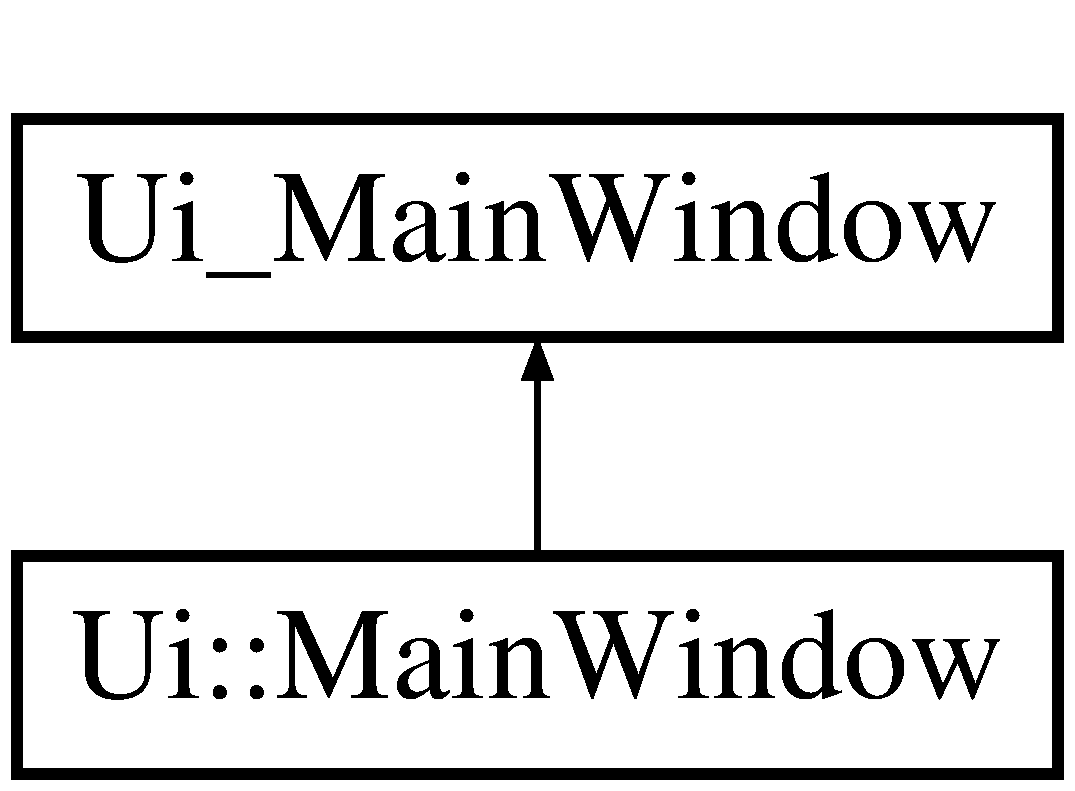
\includegraphics[height=2.000000cm]{class_ui_1_1_main_window}
\end{center}
\end{figure}
\subsection*{Additional Inherited Members}


The documentation for this class was generated from the following file\+:\begin{DoxyCompactItemize}
\item 
D\+:/\+Qt\+Program/\+Qt5/\+Fusion/ui\+\_\+mainwindow.\+h\end{DoxyCompactItemize}

\hypertarget{structstereo__vision_1_1match_param_b_m}{}\section{stereo\+\_\+vision\+:\+:match\+Param\+B\+M Struct Reference}
\label{structstereo__vision_1_1match_param_b_m}\index{stereo\+\_\+vision\+::match\+Param\+B\+M@{stereo\+\_\+vision\+::match\+Param\+B\+M}}
\subsection*{Public Attributes}
\begin{DoxyCompactItemize}
\item 
\hypertarget{structstereo__vision_1_1match_param_b_m_ac62638a82ccdb7a1f44cc59b45e96b72}{}int {\bfseries pre\+\_\+filter\+\_\+size}\label{structstereo__vision_1_1match_param_b_m_ac62638a82ccdb7a1f44cc59b45e96b72}

\item 
\hypertarget{structstereo__vision_1_1match_param_b_m_a776a38ec2db6033ce41da103144ed886}{}int {\bfseries pre\+\_\+filter\+\_\+cap}\label{structstereo__vision_1_1match_param_b_m_a776a38ec2db6033ce41da103144ed886}

\item 
\hypertarget{structstereo__vision_1_1match_param_b_m_ad6a0a391ff0b8762db62c50515545cd8}{}int {\bfseries S\+A\+D\+\_\+window\+\_\+size}\label{structstereo__vision_1_1match_param_b_m_ad6a0a391ff0b8762db62c50515545cd8}

\item 
\hypertarget{structstereo__vision_1_1match_param_b_m_a989415e74623c2af54cf91ce74c9e1c8}{}int {\bfseries min\+\_\+disp}\label{structstereo__vision_1_1match_param_b_m_a989415e74623c2af54cf91ce74c9e1c8}

\item 
\hypertarget{structstereo__vision_1_1match_param_b_m_a25d6b6ca0bb6767e6661a8a8c1391f22}{}int {\bfseries num\+\_\+of\+\_\+disp}\label{structstereo__vision_1_1match_param_b_m_a25d6b6ca0bb6767e6661a8a8c1391f22}

\item 
\hypertarget{structstereo__vision_1_1match_param_b_m_acbdc31085a4602f5a97c590ec8ff3417}{}int {\bfseries texture\+\_\+thresh}\label{structstereo__vision_1_1match_param_b_m_acbdc31085a4602f5a97c590ec8ff3417}

\item 
\hypertarget{structstereo__vision_1_1match_param_b_m_a77fc24a9e483d02a3f1a3bb3654e9b78}{}int {\bfseries uniquenese\+\_\+ratio}\label{structstereo__vision_1_1match_param_b_m_a77fc24a9e483d02a3f1a3bb3654e9b78}

\item 
\hypertarget{structstereo__vision_1_1match_param_b_m_a6661183f9b84d368b6f3b4f519499390}{}int {\bfseries speckle\+\_\+window\+\_\+size}\label{structstereo__vision_1_1match_param_b_m_a6661183f9b84d368b6f3b4f519499390}

\item 
\hypertarget{structstereo__vision_1_1match_param_b_m_a1084d18009372551eca3946d819b43f2}{}int {\bfseries speckle\+\_\+range}\label{structstereo__vision_1_1match_param_b_m_a1084d18009372551eca3946d819b43f2}

\end{DoxyCompactItemize}


The documentation for this struct was generated from the following file\+:\begin{DoxyCompactItemize}
\item 
D\+:/\+Qt\+Program/\+Qt5/\+Fusion/stereo\+\_\+vision.\+h\end{DoxyCompactItemize}

\hypertarget{structstereo__vision_1_1match_param_s_g_b_m}{}\section{stereo\+\_\+vision\+:\+:match\+Param\+S\+G\+B\+M Struct Reference}
\label{structstereo__vision_1_1match_param_s_g_b_m}\index{stereo\+\_\+vision\+::match\+Param\+S\+G\+B\+M@{stereo\+\_\+vision\+::match\+Param\+S\+G\+B\+M}}
\subsection*{Public Attributes}
\begin{DoxyCompactItemize}
\item 
\hypertarget{structstereo__vision_1_1match_param_s_g_b_m_a5140d9b4940a08c49e31f94360b05f7b}{}int {\bfseries pre\+\_\+filter\+\_\+cap}\label{structstereo__vision_1_1match_param_s_g_b_m_a5140d9b4940a08c49e31f94360b05f7b}

\item 
\hypertarget{structstereo__vision_1_1match_param_s_g_b_m_aae74dab15900400eb4c5e7645a482e9b}{}int {\bfseries S\+A\+D\+\_\+window\+\_\+size}\label{structstereo__vision_1_1match_param_s_g_b_m_aae74dab15900400eb4c5e7645a482e9b}

\item 
\hypertarget{structstereo__vision_1_1match_param_s_g_b_m_a986221639afed790475e61d6a5e48101}{}int {\bfseries min\+\_\+disp}\label{structstereo__vision_1_1match_param_s_g_b_m_a986221639afed790475e61d6a5e48101}

\item 
\hypertarget{structstereo__vision_1_1match_param_s_g_b_m_a6c922730bfbbd27d66ae55b88f77a3b3}{}int {\bfseries num\+\_\+of\+\_\+disp}\label{structstereo__vision_1_1match_param_s_g_b_m_a6c922730bfbbd27d66ae55b88f77a3b3}

\item 
\hypertarget{structstereo__vision_1_1match_param_s_g_b_m_a10bf5782f0dcda2d44657593bf72fb60}{}int {\bfseries uniquenese\+\_\+ratio}\label{structstereo__vision_1_1match_param_s_g_b_m_a10bf5782f0dcda2d44657593bf72fb60}

\item 
\hypertarget{structstereo__vision_1_1match_param_s_g_b_m_ac156150c87f5d1d496b029ee647c0f55}{}int {\bfseries speckle\+\_\+window\+\_\+size}\label{structstereo__vision_1_1match_param_s_g_b_m_ac156150c87f5d1d496b029ee647c0f55}

\item 
\hypertarget{structstereo__vision_1_1match_param_s_g_b_m_ace58309e7f00078e2cb28e8aeae69386}{}int {\bfseries speckle\+\_\+range}\label{structstereo__vision_1_1match_param_s_g_b_m_ace58309e7f00078e2cb28e8aeae69386}

\end{DoxyCompactItemize}


The documentation for this struct was generated from the following file\+:\begin{DoxyCompactItemize}
\item 
D\+:/\+Qt\+Program/\+Qt5/\+Fusion/stereo\+\_\+vision.\+h\end{DoxyCompactItemize}

\hypertarget{struct_radar_controller_1_1_e_s_r___s_t_a_t_1_1_m_e_d___r_a_n_g_e___m_o_d_e}{}\section{Radar\+Controller\+:\+:E\+S\+R\+\_\+\+S\+T\+A\+T\+:\+:M\+E\+D\+\_\+\+R\+A\+N\+G\+E\+\_\+\+M\+O\+D\+E Struct Reference}
\label{struct_radar_controller_1_1_e_s_r___s_t_a_t_1_1_m_e_d___r_a_n_g_e___m_o_d_e}\index{Radar\+Controller\+::\+E\+S\+R\+\_\+\+S\+T\+A\+T\+::\+M\+E\+D\+\_\+\+R\+A\+N\+G\+E\+\_\+\+M\+O\+D\+E@{Radar\+Controller\+::\+E\+S\+R\+\_\+\+S\+T\+A\+T\+::\+M\+E\+D\+\_\+\+R\+A\+N\+G\+E\+\_\+\+M\+O\+D\+E}}
\subsection*{Public Types}
\begin{DoxyCompactItemize}
\item 
\hypertarget{struct_radar_controller_1_1_e_s_r___s_t_a_t_1_1_m_e_d___r_a_n_g_e___m_o_d_e_aa59703ad227d33f68c1fdd4db0a61daf}{}enum \{ {\bfseries B\+O\+T\+H\+\_\+\+N\+O\+\_\+\+U\+P\+D\+A\+T\+E}, 
{\bfseries M\+R\+\_\+\+U\+P\+D\+A\+T\+E}, 
{\bfseries L\+R\+\_\+\+U\+P\+D\+A\+T\+E}, 
{\bfseries B\+O\+T\+H\+\_\+\+U\+P\+D\+A\+T\+E}
 \}\label{struct_radar_controller_1_1_e_s_r___s_t_a_t_1_1_m_e_d___r_a_n_g_e___m_o_d_e_aa59703ad227d33f68c1fdd4db0a61daf}

\end{DoxyCompactItemize}


The documentation for this struct was generated from the following file\+:\begin{DoxyCompactItemize}
\item 
D\+:/\+Qt\+Program/\+Qt5/\+Fusion/radarcontroller.\+h\end{DoxyCompactItemize}

\hypertarget{class_mouse_label}{}\section{Mouse\+Label Class Reference}
\label{class_mouse_label}\index{Mouse\+Label@{Mouse\+Label}}
Inheritance diagram for Mouse\+Label\+:\begin{figure}[H]
\begin{center}
\leavevmode
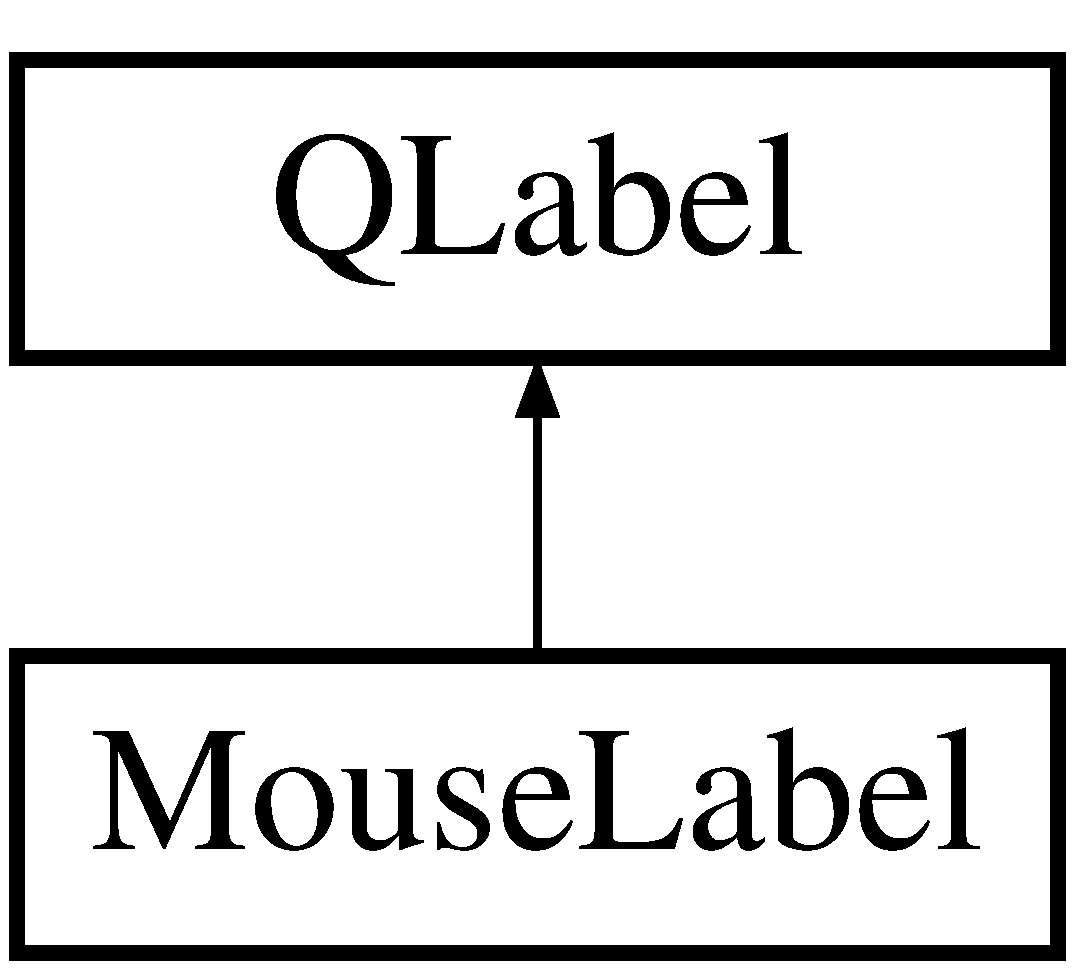
\includegraphics[height=2.000000cm]{class_mouse_label}
\end{center}
\end{figure}
\subsection*{Signals}
\begin{DoxyCompactItemize}
\item 
\hypertarget{class_mouse_label_a19b8735425fefa355e5707b9ef31ff04}{}void {\bfseries m\+X\+Y} (int x, int y)\label{class_mouse_label_a19b8735425fefa355e5707b9ef31ff04}

\end{DoxyCompactItemize}
\subsection*{Public Member Functions}
\begin{DoxyCompactItemize}
\item 
\hypertarget{class_mouse_label_a9d790b509217e61306591091bafb0d3f}{}{\bfseries Mouse\+Label} (Q\+Widget $\ast$parent=0)\label{class_mouse_label_a9d790b509217e61306591091bafb0d3f}

\end{DoxyCompactItemize}
\subsection*{Protected Member Functions}
\begin{DoxyCompactItemize}
\item 
\hypertarget{class_mouse_label_a66b5f68b628a65461b1cd773ad6dad13}{}virtual void {\bfseries mouse\+Move\+Event} (Q\+Mouse\+Event $\ast$e)\label{class_mouse_label_a66b5f68b628a65461b1cd773ad6dad13}

\end{DoxyCompactItemize}


The documentation for this class was generated from the following files\+:\begin{DoxyCompactItemize}
\item 
D\+:/\+Qt\+Program/\+Qt5/\+Fusion/mainwindow.\+h\item 
D\+:/\+Qt\+Program/\+Qt5/\+Fusion/mainwindow.\+cpp\end{DoxyCompactItemize}

\hypertarget{structstereo__vision_1_1object_info}{}\section{stereo\+\_\+vision\+:\+:object\+Info Struct Reference}
\label{structstereo__vision_1_1object_info}\index{stereo\+\_\+vision\+::object\+Info@{stereo\+\_\+vision\+::object\+Info}}
\subsection*{Public Attributes}
\begin{DoxyCompactItemize}
\item 
\hypertarget{structstereo__vision_1_1object_info_a86477a8593132539bd62a97dcefd8222}{}int {\bfseries pts\+\_\+num}\label{structstereo__vision_1_1object_info_a86477a8593132539bd62a97dcefd8222}

\item 
\hypertarget{structstereo__vision_1_1object_info_ad508298c68abd33e4dac728d447d0ba4}{}bool {\bfseries labeled}\label{structstereo__vision_1_1object_info_ad508298c68abd33e4dac728d447d0ba4}

\item 
\hypertarget{structstereo__vision_1_1object_info_ad0907414a1af2544d9d7949481bf70c5}{}float {\bfseries avg\+\_\+\+Z}\label{structstereo__vision_1_1object_info_ad0907414a1af2544d9d7949481bf70c5}

\item 
\hypertarget{structstereo__vision_1_1object_info_a29a79b6657553d64b5a31d88508fe9aa}{}float {\bfseries avg\+\_\+\+X}\label{structstereo__vision_1_1object_info_a29a79b6657553d64b5a31d88508fe9aa}

\item 
\hypertarget{structstereo__vision_1_1object_info_a5fd0b0149e40b8d7cdab51f67fdf4c18}{}float {\bfseries avg\+\_\+\+Y}\label{structstereo__vision_1_1object_info_a5fd0b0149e40b8d7cdab51f67fdf4c18}

\item 
\hypertarget{structstereo__vision_1_1object_info_a8b4a88c1db9929bf9b9befa081e99c98}{}cv\+::\+Point {\bfseries rect\+\_\+tl}\label{structstereo__vision_1_1object_info_a8b4a88c1db9929bf9b9befa081e99c98}

\item 
\hypertarget{structstereo__vision_1_1object_info_ac38fdc320a13a6390b5ecdb490771689}{}cv\+::\+Point {\bfseries rect\+\_\+br}\label{structstereo__vision_1_1object_info_ac38fdc320a13a6390b5ecdb490771689}

\item 
\hypertarget{structstereo__vision_1_1object_info_a8f3f37c5fcbc13c1d2d23cae5bb0385e}{}std\+::pair$<$ int, int $>$ {\bfseries tl}\label{structstereo__vision_1_1object_info_a8f3f37c5fcbc13c1d2d23cae5bb0385e}

\item 
\hypertarget{structstereo__vision_1_1object_info_a814c65b1c8922b7078a0c8154ac98910}{}std\+::pair$<$ int, int $>$ {\bfseries br}\label{structstereo__vision_1_1object_info_a814c65b1c8922b7078a0c8154ac98910}

\item 
\hypertarget{structstereo__vision_1_1object_info_a2793afa44eb5812695e886a4728e4a9d}{}std\+::pair$<$ int, int $>$ {\bfseries center}\label{structstereo__vision_1_1object_info_a2793afa44eb5812695e886a4728e4a9d}

\item 
\hypertarget{structstereo__vision_1_1object_info_a6aefe3c6053dbcd33495f030571a3f31}{}cv\+::\+Scalar {\bfseries color}\label{structstereo__vision_1_1object_info_a6aefe3c6053dbcd33495f030571a3f31}

\item 
\hypertarget{structstereo__vision_1_1object_info_afb1502d96fe35b0758f01d8176ec91ec}{}cv\+::\+Mat {\bfseries img}\label{structstereo__vision_1_1object_info_afb1502d96fe35b0758f01d8176ec91ec}

\item 
\hypertarget{structstereo__vision_1_1object_info_a14395c5a5315c3a662702a92a35cb2e8}{}cv\+::\+Rect {\bfseries rect}\label{structstereo__vision_1_1object_info_a14395c5a5315c3a662702a92a35cb2e8}

\item 
\hypertarget{structstereo__vision_1_1object_info_a21a31b9a8854dd0cc58ae2eb4434779a}{}\hyperlink{struct_sensor_base_1_1_p_c}{P\+C} {\bfseries pc}\label{structstereo__vision_1_1object_info_a21a31b9a8854dd0cc58ae2eb4434779a}

\item 
\hypertarget{structstereo__vision_1_1object_info_a27f555ff0489bd67eac034d0ca6681d4}{}cv\+::\+Rect {\bfseries rect\+\_\+f}\label{structstereo__vision_1_1object_info_a27f555ff0489bd67eac034d0ca6681d4}

\item 
\hypertarget{structstereo__vision_1_1object_info_aafa09d6e6e70b2be7c95cf9d3195461a}{}cv\+::\+Point {\bfseries plot\+\_\+pt\+\_\+f}\label{structstereo__vision_1_1object_info_aafa09d6e6e70b2be7c95cf9d3195461a}

\item 
\hypertarget{structstereo__vision_1_1object_info_a92e197f82126dcc5d1fd9de28e176a6d}{}cv\+::\+Rect {\bfseries rect\+\_\+world}\label{structstereo__vision_1_1object_info_a92e197f82126dcc5d1fd9de28e176a6d}

\item 
\hypertarget{structstereo__vision_1_1object_info_af40296f15626dd59bbb7e03e58700125}{}\hyperlink{struct_sensor_base_1_1_p_c}{P\+C} {\bfseries pc\+\_\+world}\label{structstereo__vision_1_1object_info_af40296f15626dd59bbb7e03e58700125}

\end{DoxyCompactItemize}


The documentation for this struct was generated from the following file\+:\begin{DoxyCompactItemize}
\item 
D\+:/\+Qt\+Program/\+Qt5/\+Fusion/stereo\+\_\+vision.\+h\end{DoxyCompactItemize}

\hypertarget{class_object_recognition}{}\section{Object\+Recognition Class Reference}
\label{class_object_recognition}\index{Object\+Recognition@{Object\+Recognition}}


The documentation for this class was generated from the following files\+:\begin{DoxyCompactItemize}
\item 
D\+:/\+Qt\+Program/\+Qt5/\+Fusion/objectrecognition.\+h\item 
D\+:/\+Qt\+Program/\+Qt5/\+Fusion/objectrecognition.\+cpp\end{DoxyCompactItemize}

\hypertarget{struct_radar_controller_1_1object_tracking_info}{}\section{Radar\+Controller\+:\+:object\+Tracking\+Info Struct Reference}
\label{struct_radar_controller_1_1object_tracking_info}\index{Radar\+Controller\+::object\+Tracking\+Info@{Radar\+Controller\+::object\+Tracking\+Info}}
\subsection*{Public Attributes}
\begin{DoxyCompactItemize}
\item 
\hypertarget{struct_radar_controller_1_1object_tracking_info_a2aaf3920cd5901ba0f391d9b42d2b838}{}float \hyperlink{struct_radar_controller_1_1object_tracking_info_a2aaf3920cd5901ba0f391d9b42d2b838}{angle}\label{struct_radar_controller_1_1object_tracking_info_a2aaf3920cd5901ba0f391d9b42d2b838}

\begin{DoxyCompactList}\small\item\em azimuth degree. Middle is zero. From -\/51.\+2 to 51.\+1. (degree) \end{DoxyCompactList}\item 
\hypertarget{struct_radar_controller_1_1object_tracking_info_a35f6e4d0a62549c38398b7a0ed62790e}{}bool \hyperlink{struct_radar_controller_1_1object_tracking_info_a35f6e4d0a62549c38398b7a0ed62790e}{bridge\+\_\+object}\label{struct_radar_controller_1_1object_tracking_info_a35f6e4d0a62549c38398b7a0ed62790e}

\begin{DoxyCompactList}\small\item\em non-\/functional \end{DoxyCompactList}\item 
\hypertarget{struct_radar_controller_1_1object_tracking_info_a5a0db9722daf21aee6d5ca53fb058458}{}bool {\bfseries grouping\+\_\+changed}\label{struct_radar_controller_1_1object_tracking_info_a5a0db9722daf21aee6d5ca53fb058458}

\item 
float \hyperlink{struct_radar_controller_1_1object_tracking_info_a232c799e920e93faac192726993f32cd}{lat\+\_\+rate}
\item 
\hypertarget{struct_radar_controller_1_1object_tracking_info_a3869b7891b8eb1745f48d480e9a4c259}{}int {\bfseries med\+\_\+range\+\_\+mode}\label{struct_radar_controller_1_1object_tracking_info_a3869b7891b8eb1745f48d480e9a4c259}

\item 
\hypertarget{struct_radar_controller_1_1object_tracking_info_a679bf8c6b434c3a386db0204e64cd245}{}bool {\bfseries oncoming}\label{struct_radar_controller_1_1object_tracking_info_a679bf8c6b434c3a386db0204e64cd245}

\item 
float \hyperlink{struct_radar_controller_1_1object_tracking_info_a09342f3b1f19b9c9f188d912ebc54371}{range}
\item 
float \hyperlink{struct_radar_controller_1_1object_tracking_info_ae5b537d910d05bbf716c5a38b8677eed}{range\+\_\+accel}
\item 
float \hyperlink{struct_radar_controller_1_1object_tracking_info_a52d996bdc367f363dada5af01960171b}{range\+\_\+rate}
\item 
\hypertarget{struct_radar_controller_1_1object_tracking_info_a8e756168e451e21714ea824cd27ff3e8}{}bool {\bfseries rolling\+\_\+count}\label{struct_radar_controller_1_1object_tracking_info_a8e756168e451e21714ea824cd27ff3e8}

\item 
\hypertarget{struct_radar_controller_1_1object_tracking_info_a65bf279bcc533321be393aef4b823b8f}{}int {\bfseries status}\label{struct_radar_controller_1_1object_tracking_info_a65bf279bcc533321be393aef4b823b8f}

\item 
\hypertarget{struct_radar_controller_1_1object_tracking_info_a446630a4ec96aaa9098007ad3e465f85}{}float \hyperlink{struct_radar_controller_1_1object_tracking_info_a446630a4ec96aaa9098007ad3e465f85}{width}\label{struct_radar_controller_1_1object_tracking_info_a446630a4ec96aaa9098007ad3e465f85}

\begin{DoxyCompactList}\small\item\em non-\/functional \end{DoxyCompactList}\item 
\hypertarget{struct_radar_controller_1_1object_tracking_info_a4199132f9159ef104b899b75ffa75a10}{}double \hyperlink{struct_radar_controller_1_1object_tracking_info_a4199132f9159ef104b899b75ffa75a10}{x}\label{struct_radar_controller_1_1object_tracking_info_a4199132f9159ef104b899b75ffa75a10}

\begin{DoxyCompactList}\small\item\em radar coordinates system (m) \end{DoxyCompactList}\item 
\hypertarget{struct_radar_controller_1_1object_tracking_info_ad65229192d33702324ea63d473d5c5f6}{}double {\bfseries y}\label{struct_radar_controller_1_1object_tracking_info_ad65229192d33702324ea63d473d5c5f6}

\item 
\hypertarget{struct_radar_controller_1_1object_tracking_info_aeabaee0c1e87b4778fe3ef73fb94fff0}{}double {\bfseries z}\label{struct_radar_controller_1_1object_tracking_info_aeabaee0c1e87b4778fe3ef73fb94fff0}

\item 
\hypertarget{struct_radar_controller_1_1object_tracking_info_a4db7135ba2efd70e29c1f0a4fe74e738}{}bool \hyperlink{struct_radar_controller_1_1object_tracking_info_a4db7135ba2efd70e29c1f0a4fe74e738}{fg\+\_\+fused}\label{struct_radar_controller_1_1object_tracking_info_a4db7135ba2efd70e29c1f0a4fe74e738}

\begin{DoxyCompactList}\small\item\em Is object fused with stereo vision or not. \end{DoxyCompactList}\item 
\hypertarget{struct_radar_controller_1_1object_tracking_info_ae1486f6ad1c7fcd43c36bbf1ef51f923}{}\hyperlink{struct_sensor_base_1_1_p_c}{P\+C} {\bfseries pc}\label{struct_radar_controller_1_1object_tracking_info_ae1486f6ad1c7fcd43c36bbf1ef51f923}

\item 
\hypertarget{struct_radar_controller_1_1object_tracking_info_afd14a9321bcf9d0e215cb980f48d871b}{}cv\+::\+Point \hyperlink{struct_radar_controller_1_1object_tracking_info_afd14a9321bcf9d0e215cb980f48d871b}{plot\+\_\+pt\+\_\+f}\label{struct_radar_controller_1_1object_tracking_info_afd14a9321bcf9d0e215cb980f48d871b}

\begin{DoxyCompactList}\small\item\em (pixel) \end{DoxyCompactList}\item 
\hypertarget{struct_radar_controller_1_1object_tracking_info_abf098a63453796c5e20138155b9681f2}{}\hyperlink{struct_sensor_base_1_1_p_c}{P\+C} \hyperlink{struct_radar_controller_1_1object_tracking_info_abf098a63453796c5e20138155b9681f2}{pc\+\_\+world}\label{struct_radar_controller_1_1object_tracking_info_abf098a63453796c5e20138155b9681f2}

\begin{DoxyCompactList}\small\item\em (cm) \end{DoxyCompactList}\end{DoxyCompactItemize}


\subsection{Member Data Documentation}
\hypertarget{struct_radar_controller_1_1object_tracking_info_a232c799e920e93faac192726993f32cd}{}\index{Radar\+Controller\+::object\+Tracking\+Info@{Radar\+Controller\+::object\+Tracking\+Info}!lat\+\_\+rate@{lat\+\_\+rate}}
\index{lat\+\_\+rate@{lat\+\_\+rate}!Radar\+Controller\+::object\+Tracking\+Info@{Radar\+Controller\+::object\+Tracking\+Info}}
\subsubsection[{lat\+\_\+rate}]{\setlength{\rightskip}{0pt plus 5cm}float Radar\+Controller\+::object\+Tracking\+Info\+::lat\+\_\+rate}\label{struct_radar_controller_1_1object_tracking_info_a232c799e920e93faac192726993f32cd}

\begin{DoxyItemize}
\item is counter clockwise. (m/s) 
\end{DoxyItemize}\hypertarget{struct_radar_controller_1_1object_tracking_info_a09342f3b1f19b9c9f188d912ebc54371}{}\index{Radar\+Controller\+::object\+Tracking\+Info@{Radar\+Controller\+::object\+Tracking\+Info}!range@{range}}
\index{range@{range}!Radar\+Controller\+::object\+Tracking\+Info@{Radar\+Controller\+::object\+Tracking\+Info}}
\subsubsection[{range}]{\setlength{\rightskip}{0pt plus 5cm}float Radar\+Controller\+::object\+Tracking\+Info\+::range}\label{struct_radar_controller_1_1object_tracking_info_a09342f3b1f19b9c9f188d912ebc54371}

\begin{DoxyItemize}
\item is away. (m) 
\end{DoxyItemize}\hypertarget{struct_radar_controller_1_1object_tracking_info_ae5b537d910d05bbf716c5a38b8677eed}{}\index{Radar\+Controller\+::object\+Tracking\+Info@{Radar\+Controller\+::object\+Tracking\+Info}!range\+\_\+accel@{range\+\_\+accel}}
\index{range\+\_\+accel@{range\+\_\+accel}!Radar\+Controller\+::object\+Tracking\+Info@{Radar\+Controller\+::object\+Tracking\+Info}}
\subsubsection[{range\+\_\+accel}]{\setlength{\rightskip}{0pt plus 5cm}float Radar\+Controller\+::object\+Tracking\+Info\+::range\+\_\+accel}\label{struct_radar_controller_1_1object_tracking_info_ae5b537d910d05bbf716c5a38b8677eed}

\begin{DoxyItemize}
\item is away. (m/s$^\wedge$2) 
\end{DoxyItemize}\hypertarget{struct_radar_controller_1_1object_tracking_info_a52d996bdc367f363dada5af01960171b}{}\index{Radar\+Controller\+::object\+Tracking\+Info@{Radar\+Controller\+::object\+Tracking\+Info}!range\+\_\+rate@{range\+\_\+rate}}
\index{range\+\_\+rate@{range\+\_\+rate}!Radar\+Controller\+::object\+Tracking\+Info@{Radar\+Controller\+::object\+Tracking\+Info}}
\subsubsection[{range\+\_\+rate}]{\setlength{\rightskip}{0pt plus 5cm}float Radar\+Controller\+::object\+Tracking\+Info\+::range\+\_\+rate}\label{struct_radar_controller_1_1object_tracking_info_a52d996bdc367f363dada5af01960171b}

\begin{DoxyItemize}
\item is away. (m/s) 
\end{DoxyItemize}

The documentation for this struct was generated from the following file\+:\begin{DoxyCompactItemize}
\item 
D\+:/\+Qt\+Program/\+Qt5/\+Fusion/radarcontroller.\+h\end{DoxyCompactItemize}

\hypertarget{struct_radar_controller_1_1_e_s_r___s_t_a_t_1_1_o_n_c_o_m_i_n_g}{}\section{Radar\+Controller\+:\+:E\+S\+R\+\_\+\+S\+T\+A\+T\+:\+:O\+N\+C\+O\+M\+I\+N\+G Struct Reference}
\label{struct_radar_controller_1_1_e_s_r___s_t_a_t_1_1_o_n_c_o_m_i_n_g}\index{Radar\+Controller\+::\+E\+S\+R\+\_\+\+S\+T\+A\+T\+::\+O\+N\+C\+O\+M\+I\+N\+G@{Radar\+Controller\+::\+E\+S\+R\+\_\+\+S\+T\+A\+T\+::\+O\+N\+C\+O\+M\+I\+N\+G}}
\subsection*{Public Types}
\begin{DoxyCompactItemize}
\item 
\hypertarget{struct_radar_controller_1_1_e_s_r___s_t_a_t_1_1_o_n_c_o_m_i_n_g_af5034e800ce0a23b07afe148745d4b0d}{}enum \{ {\bfseries N\+O} = false, 
{\bfseries Y\+E\+S} = true
 \}\label{struct_radar_controller_1_1_e_s_r___s_t_a_t_1_1_o_n_c_o_m_i_n_g_af5034e800ce0a23b07afe148745d4b0d}

\end{DoxyCompactItemize}


The documentation for this struct was generated from the following file\+:\begin{DoxyCompactItemize}
\item 
D\+:/\+Qt\+Program/\+Qt5/\+Fusion/radarcontroller.\+h\end{DoxyCompactItemize}

\hypertarget{struct_sensor_base_1_1_p_c}{}\section{Sensor\+Base\+:\+:P\+C Struct Reference}
\label{struct_sensor_base_1_1_p_c}\index{Sensor\+Base\+::\+P\+C@{Sensor\+Base\+::\+P\+C}}
\subsection*{Public Member Functions}
\begin{DoxyCompactItemize}
\item 
\hypertarget{struct_sensor_base_1_1_p_c_a819e15c82afbf3c4b067782bad37b121}{}{\bfseries P\+C} (double \hyperlink{struct_sensor_base_1_1_p_c_a886d9de0b686ead3b6a1685b1bbd7304}{range}=0.\+0, double \hyperlink{struct_sensor_base_1_1_p_c_aba431354726e699601060c94ff865180}{angle}=0.\+0)\label{struct_sensor_base_1_1_p_c_a819e15c82afbf3c4b067782bad37b121}

\end{DoxyCompactItemize}
\subsection*{Public Attributes}
\begin{DoxyCompactItemize}
\item 
double \hyperlink{struct_sensor_base_1_1_p_c_aba431354726e699601060c94ff865180}{angle}
\item 
\hypertarget{struct_sensor_base_1_1_p_c_a886d9de0b686ead3b6a1685b1bbd7304}{}double \hyperlink{struct_sensor_base_1_1_p_c_a886d9de0b686ead3b6a1685b1bbd7304}{range}\label{struct_sensor_base_1_1_p_c_a886d9de0b686ead3b6a1685b1bbd7304}

\begin{DoxyCompactList}\small\item\em (cm) \end{DoxyCompactList}\end{DoxyCompactItemize}


\subsection{Member Data Documentation}
\hypertarget{struct_sensor_base_1_1_p_c_aba431354726e699601060c94ff865180}{}\index{Sensor\+Base\+::\+P\+C@{Sensor\+Base\+::\+P\+C}!angle@{angle}}
\index{angle@{angle}!Sensor\+Base\+::\+P\+C@{Sensor\+Base\+::\+P\+C}}
\subsubsection[{angle}]{\setlength{\rightskip}{0pt plus 5cm}double Sensor\+Base\+::\+P\+C\+::angle}\label{struct_sensor_base_1_1_p_c_aba431354726e699601060c94ff865180}
orientation degree (degree). Forward is set as zero and counting clockwisely. 

The documentation for this struct was generated from the following file\+:\begin{DoxyCompactItemize}
\item 
D\+:/\+Qt\+Program/\+Qt5/\+Fusion/sensorbase.\+h\end{DoxyCompactItemize}

\hypertarget{class_radar_controller}{}\section{Radar\+Controller Class Reference}
\label{class_radar_controller}\index{Radar\+Controller@{Radar\+Controller}}


The \hyperlink{class_radar_controller}{Radar\+Controller} class.  




{\ttfamily \#include $<$radarcontroller.\+h$>$}

Inheritance diagram for Radar\+Controller\+:\begin{figure}[H]
\begin{center}
\leavevmode
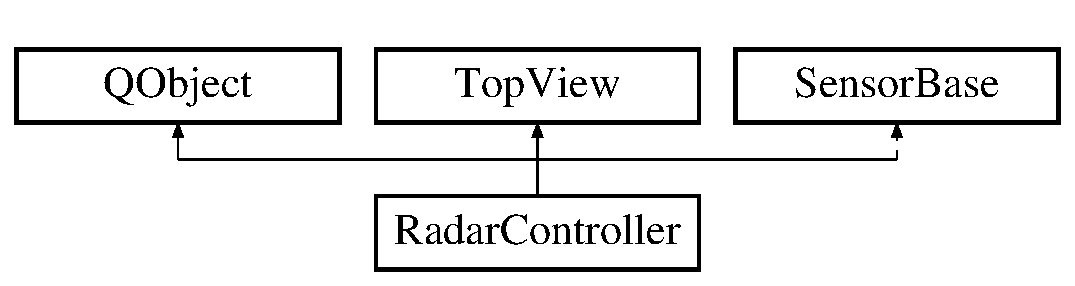
\includegraphics[height=2.000000cm]{class_radar_controller}
\end{center}
\end{figure}
\subsection*{Classes}
\begin{DoxyCompactItemize}
\item 
struct \hyperlink{struct_radar_controller_1_1_e_s_r___s_t_a_t}{E\+S\+R\+\_\+\+S\+T\+A\+T}
\item 
struct \hyperlink{struct_radar_controller_1_1object_tracking_info}{object\+Tracking\+Info}
\end{DoxyCompactItemize}
\subsection*{Signals}
\begin{DoxyCompactItemize}
\item 
\hypertarget{class_radar_controller_af732d231a09db2453b425d49fc4ff80e}{}void {\bfseries update\+G\+U\+I} (int detected\+\_\+obj, cv\+::\+Mat $\ast$img, cv\+::\+Mat $\ast$\hyperlink{class_top_view_a693454cfb21851b389634e28bdabe35a}{topview})\label{class_radar_controller_af732d231a09db2453b425d49fc4ff80e}

\item 
\hypertarget{class_radar_controller_a9fd04ef43fb1300abcb125fc02a44779}{}void {\bfseries data\+End} ()\label{class_radar_controller_a9fd04ef43fb1300abcb125fc02a44779}

\end{DoxyCompactItemize}
\subsection*{Public Member Functions}
\begin{DoxyCompactItemize}
\item 
bool \hyperlink{class_radar_controller_a0d77375448b211c62fd7de55f1ddd029}{open} ()
\begin{DoxyCompactList}\small\item\em open the radar w/ C\+A\+N Bus \end{DoxyCompactList}\item 
bool \hyperlink{class_radar_controller_a09975f3f18fd13a533666800a5ff5b24}{write} ()
\begin{DoxyCompactList}\small\item\em write msg into the radar \end{DoxyCompactList}\item 
\hypertarget{class_radar_controller_acff63260ffa92857f1d1e4c44ea3fc4d}{}void \hyperlink{class_radar_controller_acff63260ffa92857f1d1e4c44ea3fc4d}{bus\+On} ()\label{class_radar_controller_acff63260ffa92857f1d1e4c44ea3fc4d}

\begin{DoxyCompactList}\small\item\em bus\+On starts communication interface \end{DoxyCompactList}\item 
\hypertarget{class_radar_controller_aaa344f45e0ca4cae204ff660e1b5d56f}{}void \hyperlink{class_radar_controller_aaa344f45e0ca4cae204ff660e1b5d56f}{bus\+Off} ()\label{class_radar_controller_aaa344f45e0ca4cae204ff660e1b5d56f}

\begin{DoxyCompactList}\small\item\em bus\+Off closes communication interface \end{DoxyCompactList}\item 
\hypertarget{class_radar_controller_aad3c48136e50bb70d2b222c480b1ff63}{}void \hyperlink{class_radar_controller_aad3c48136e50bb70d2b222c480b1ff63}{retrieving\+Data} ()\label{class_radar_controller_aad3c48136e50bb70d2b222c480b1ff63}

\begin{DoxyCompactList}\small\item\em retrieving\+Data starts retrieving data \end{DoxyCompactList}\item 
\hypertarget{class_radar_controller_a022a0e55af4aff4f57c46af3ced689e7}{}int {\bfseries data\+Exec} ()\label{class_radar_controller_a022a0e55af4aff4f57c46af3ced689e7}

\item 
\hypertarget{class_radar_controller_a4f5826b99e3bc782a2c08666ae93975f}{}int {\bfseries gui\+Update} ()\label{class_radar_controller_a4f5826b99e3bc782a2c08666ae93975f}

\item 
\hypertarget{class_radar_controller_ab5b5a998babad28a5b95ea542bda2c58}{}bool {\bfseries fused\+Topview} ()\label{class_radar_controller_ab5b5a998babad28a5b95ea542bda2c58}

\item 
\hypertarget{class_radar_controller_ab29f8d8b1be90335d003b60d18665058}{}bool {\bfseries is\+Opened} ()\label{class_radar_controller_ab29f8d8b1be90335d003b60d18665058}

\item 
int \hyperlink{class_radar_controller_ae7d9c576fef7e4ead101de05470bca8e}{obj\+Size} ()
\begin{DoxyCompactList}\small\item\em obj\+Size \end{DoxyCompactList}\item 
\hypertarget{class_radar_controller_af15a6be956315b8160ed80fa16e08416}{}void {\bfseries update\+Data\+For\+Display} ()\label{class_radar_controller_af15a6be956315b8160ed80fa16e08416}

\end{DoxyCompactItemize}
\subsection*{Public Attributes}
\begin{DoxyCompactItemize}
\item 
\hypertarget{class_radar_controller_ab393942663adff0c31ede28c791d96e0}{}int {\bfseries time\+\_\+proc}\label{class_radar_controller_ab393942663adff0c31ede28c791d96e0}

\item 
\hypertarget{class_radar_controller_a9a911db3343eef6f1d90a4cac9118da3}{}int \hyperlink{class_radar_controller_a9a911db3343eef6f1d90a4cac9118da3}{input\+\_\+mode}\label{class_radar_controller_a9a911db3343eef6f1d90a4cac9118da3}

\begin{DoxyCompactList}\small\item\em process time of all exec. \end{DoxyCompactList}\item 
\hypertarget{class_radar_controller_a7f7b2abe18e175eaf55e3c6defcd0d22}{}Q\+Standard\+Item $\ast$ {\bfseries item}\label{class_radar_controller_a7f7b2abe18e175eaf55e3c6defcd0d22}

\item 
\hypertarget{class_radar_controller_a4ad550185a11d28e858e35aaef0b3c5b}{}bool \hyperlink{class_radar_controller_a4ad550185a11d28e858e35aaef0b3c5b}{fg\+\_\+topview}\label{class_radar_controller_a4ad550185a11d28e858e35aaef0b3c5b}

\begin{DoxyCompactList}\small\item\em check wether project to topview \end{DoxyCompactList}\item 
\hypertarget{class_radar_controller_a7fea3e37741df4cd44872e2d79e12e9f}{}int {\bfseries current\+\_\+count}\label{class_radar_controller_a7fea3e37741df4cd44872e2d79e12e9f}

\item 
\hypertarget{class_radar_controller_a8661918ec38107b526997b5f9e41faf3}{}int {\bfseries update\+\_\+count}\label{class_radar_controller_a8661918ec38107b526997b5f9e41faf3}

\item 
\hypertarget{class_radar_controller_a995fcdaa4d1637ab4bdf5044cbc135f1}{}\hyperlink{struct_radar_controller_1_1object_tracking_info}{object\+Tracking\+Info} $\ast$ {\bfseries objects\+\_\+display}\label{class_radar_controller_a995fcdaa4d1637ab4bdf5044cbc135f1}

\item 
\hypertarget{class_radar_controller_a3167e51817e082ef4719ee3096ac924a}{}int {\bfseries detected\+\_\+obj}\label{class_radar_controller_a3167e51817e082ef4719ee3096ac924a}

\item 
\hypertarget{class_radar_controller_a66f48c02ff32145acfb7152974d2eabe}{}int \hyperlink{class_radar_controller_a66f48c02ff32145acfb7152974d2eabe}{obj\+\_\+status\+\_\+filtered}\label{class_radar_controller_a66f48c02ff32145acfb7152974d2eabe}

\begin{DoxyCompactList}\small\item\em depends on the status (C\+A\+N\+\_\+\+T\+X\+\_\+\+T\+R\+A\+C\+K\+\_\+\+S\+T\+A\+T\+U\+S) \end{DoxyCompactList}\item 
\hypertarget{class_radar_controller_a55f807e3cc67057ee533b0b62c3e2897}{}cv\+::\+Mat {\bfseries img\+\_\+radar}\label{class_radar_controller_a55f807e3cc67057ee533b0b62c3e2897}

\item 
\hypertarget{class_radar_controller_a2d1a8c95498afd084483ba8181f7857b}{}cv\+::\+Mat {\bfseries img\+\_\+radar\+\_\+\+B\+G}\label{class_radar_controller_a2d1a8c95498afd084483ba8181f7857b}

\end{DoxyCompactItemize}
\subsection*{Private Member Functions}
\begin{DoxyCompactItemize}
\item 
\hypertarget{class_radar_controller_a33369997a716834141f2706d5b88d0be}{}void {\bfseries create\+L\+U\+T} ()\label{class_radar_controller_a33369997a716834141f2706d5b88d0be}

\item 
\hypertarget{class_radar_controller_a99bcb7535e79bd1152a46013bd37a82a}{}int {\bfseries corr\+Grid\+Row} (int \hyperlink{class_top_view_a1f2b530e7979db621630dbbf9f5def15}{k})\label{class_radar_controller_a99bcb7535e79bd1152a46013bd37a82a}

\item 
\hypertarget{class_radar_controller_aaa845fcc3797bf9c4d0668236388decb}{}int {\bfseries corr\+Grid\+Col} (int \hyperlink{class_top_view_a1f2b530e7979db621630dbbf9f5def15}{k})\label{class_radar_controller_aaa845fcc3797bf9c4d0668236388decb}

\item 
\hypertarget{class_radar_controller_ad93fa3a9ec75d9f3bb9f4ad0a75ae006}{}void {\bfseries reset} ()\label{class_radar_controller_ad93fa3a9ec75d9f3bb9f4ad0a75ae006}

\item 
\hypertarget{class_radar_controller_af7eaac873ac1f4fc746c0d9cd31d248c}{}bool {\bfseries data\+In} ()\label{class_radar_controller_af7eaac873ac1f4fc746c0d9cd31d248c}

\item 
\hypertarget{class_radar_controller_a0d6d498d176e09a3ab6078950ff6e275}{}void {\bfseries draw\+Front\+View} ()\label{class_radar_controller_a0d6d498d176e09a3ab6078950ff6e275}

\item 
\hypertarget{class_radar_controller_aad4969066e1eab064e99d3bbcb8d2497}{}void {\bfseries point\+Display\+Front\+View} ()\label{class_radar_controller_aad4969066e1eab064e99d3bbcb8d2497}

\item 
\hypertarget{class_radar_controller_aed3a2fd37be354f86dc0be65957a662a}{}void {\bfseries point\+Project\+Top\+View} ()\label{class_radar_controller_aed3a2fd37be354f86dc0be65957a662a}

\end{DoxyCompactItemize}
\subsection*{Private Attributes}
\begin{DoxyCompactItemize}
\item 
\hypertarget{class_radar_controller_aff699044dcd4672775f58dc4fe2ccf84}{}\hyperlink{struct_radar_controller_1_1object_tracking_info}{object\+Tracking\+Info} $\ast$ {\bfseries objects}\label{class_radar_controller_aff699044dcd4672775f58dc4fe2ccf84}

\item 
\hypertarget{class_radar_controller_a5731c9a9aa92dca4fb6e7d8945c6fc77}{}int $\ast$ {\bfseries L\+U\+T\+\_\+grid\+\_\+row}\label{class_radar_controller_a5731c9a9aa92dca4fb6e7d8945c6fc77}

\item 
\hypertarget{class_radar_controller_ae7c1cc7fb686934ee5bf3ad4c0405beb}{}int $\ast$ {\bfseries L\+U\+T\+\_\+grid\+\_\+col}\label{class_radar_controller_ae7c1cc7fb686934ee5bf3ad4c0405beb}

\item 
\hypertarget{class_radar_controller_a2ac1b27095720c117a4c6313337ad727}{}int {\bfseries col\+\_\+shift\+\_\+\+L\+U\+T}\label{class_radar_controller_a2ac1b27095720c117a4c6313337ad727}

\item 
\hypertarget{class_radar_controller_a79de524bcd0f368e4aac579f4c6435a5}{}Q\+Time \hyperlink{class_radar_controller_a79de524bcd0f368e4aac579f4c6435a5}{t\+\_\+p}\label{class_radar_controller_a79de524bcd0f368e4aac579f4c6435a5}

\begin{DoxyCompactList}\small\item\em process time of all exec. \end{DoxyCompactList}\item 
\hypertarget{class_radar_controller_ad65c0769ca317700a173dc3b74d71b66}{}can\+Handle {\bfseries h}\label{class_radar_controller_ad65c0769ca317700a173dc3b74d71b66}

\item 
\hypertarget{class_radar_controller_aa43cb2f174f975357f10197ae6a697c6}{}can\+Status \hyperlink{class_radar_controller_aa43cb2f174f975357f10197ae6a697c6}{stat}\label{class_radar_controller_aa43cb2f174f975357f10197ae6a697c6}

\begin{DoxyCompactList}\small\item\em current C\+A\+N status \end{DoxyCompactList}\item 
\hypertarget{class_radar_controller_ac9be6d45d8c0c7599167d2b7a1a0c832}{}Q\+Time \hyperlink{class_radar_controller_ac9be6d45d8c0c7599167d2b7a1a0c832}{t}\label{class_radar_controller_ac9be6d45d8c0c7599167d2b7a1a0c832}

\begin{DoxyCompactList}\small\item\em control gui not to update too fast \end{DoxyCompactList}\item 
\hypertarget{class_radar_controller_aff4f59e6ef4610ed4ff7aba7f0e1d154}{}int {\bfseries time\+\_\+gap}\label{class_radar_controller_aff4f59e6ef4610ed4ff7aba7f0e1d154}

\item 
\hypertarget{class_radar_controller_a09b0b1956b5a19f8ff496073a18e5276}{}bool \hyperlink{class_radar_controller_a09b0b1956b5a19f8ff496073a18e5276}{fg\+\_\+read}\label{class_radar_controller_a09b0b1956b5a19f8ff496073a18e5276}

\begin{DoxyCompactList}\small\item\em reading data \end{DoxyCompactList}\item 
\hypertarget{class_radar_controller_a3dfeff66d6c588a1db7d30a3ed4c79b4}{}bool \hyperlink{class_radar_controller_a3dfeff66d6c588a1db7d30a3ed4c79b4}{fg\+\_\+data\+\_\+in}\label{class_radar_controller_a3dfeff66d6c588a1db7d30a3ed4c79b4}

\begin{DoxyCompactList}\small\item\em data is retrievable \end{DoxyCompactList}\item 
\hypertarget{class_radar_controller_a01e5d9336215bcd6aea0f041b86433bd}{}bool {\bfseries fg\+\_\+all\+\_\+data\+\_\+in} = false\label{class_radar_controller_a01e5d9336215bcd6aea0f041b86433bd}

\item 
\hypertarget{class_radar_controller_a3f6b49eb5fbe60f18cb662a082fb61de}{}long \hyperlink{class_radar_controller_a3f6b49eb5fbe60f18cb662a082fb61de}{id}\label{class_radar_controller_a3f6b49eb5fbe60f18cb662a082fb61de}

\begin{DoxyCompactList}\small\item\em C\+A\+N bus id. \end{DoxyCompactList}\item 
\hypertarget{class_radar_controller_a2d4068e949ca0e4ee1c2a14b9565c299}{}unsigned char \hyperlink{class_radar_controller_a2d4068e949ca0e4ee1c2a14b9565c299}{can\+\_\+data} \mbox{[}8\mbox{]}\label{class_radar_controller_a2d4068e949ca0e4ee1c2a14b9565c299}

\begin{DoxyCompactList}\small\item\em C\+A\+N bus info. \end{DoxyCompactList}\item 
\hypertarget{class_radar_controller_af173d0ba04e4ad7c5c74d816b532a0ba}{}unsigned int \hyperlink{class_radar_controller_af173d0ba04e4ad7c5c74d816b532a0ba}{dlc}\label{class_radar_controller_af173d0ba04e4ad7c5c74d816b532a0ba}

\begin{DoxyCompactList}\small\item\em data length \end{DoxyCompactList}\item 
\hypertarget{class_radar_controller_abe6507d861c6ed74ac93cc690e74e625}{}unsigned int {\bfseries flag}\label{class_radar_controller_abe6507d861c6ed74ac93cc690e74e625}

\item 
\hypertarget{class_radar_controller_a235c86b043b96f8fed1e322d3041e8cd}{}D\+W\+O\+R\+D {\bfseries time}\label{class_radar_controller_a235c86b043b96f8fed1e322d3041e8cd}

\item 
\hypertarget{class_radar_controller_abd1f97e3345954539ed9f2d64fa2ea8a}{}std\+::bitset$<$ 8 $>$ \hyperlink{class_radar_controller_abd1f97e3345954539ed9f2d64fa2ea8a}{b}\label{class_radar_controller_abd1f97e3345954539ed9f2d64fa2ea8a}

\begin{DoxyCompactList}\small\item\em received data (bitset) \end{DoxyCompactList}\item 
\hypertarget{class_radar_controller_ac1faf27510539e961f7a6ff465049ea1}{}std\+::string \hyperlink{class_radar_controller_ac1faf27510539e961f7a6ff465049ea1}{bin}\label{class_radar_controller_ac1faf27510539e961f7a6ff465049ea1}

\begin{DoxyCompactList}\small\item\em received data (string) \end{DoxyCompactList}\item 
\hypertarget{class_radar_controller_ae8d2b8b7295f25282b733817fcdd242c}{}std\+::bitset$<$ 6 $>$ {\bfseries b\+\_\+track\+\_\+lat\+\_\+rate}\label{class_radar_controller_ae8d2b8b7295f25282b733817fcdd242c}

\item 
\hypertarget{class_radar_controller_a526dfd9a787864f60c4c7d8c9eae078b}{}std\+::bitset$<$ 1 $>$ {\bfseries b\+\_\+track\+\_\+grouping\+\_\+changed}\label{class_radar_controller_a526dfd9a787864f60c4c7d8c9eae078b}

\item 
\hypertarget{class_radar_controller_addf9cc22f4190ab2bc4a9b8b4d2cead7}{}std\+::bitset$<$ 1 $>$ {\bfseries b\+\_\+track\+\_\+oncoming}\label{class_radar_controller_addf9cc22f4190ab2bc4a9b8b4d2cead7}

\item 
\hypertarget{class_radar_controller_a7edb023acbee9fb877476cc0120d2e43}{}std\+::bitset$<$ 3 $>$ {\bfseries b\+\_\+track\+\_\+status}\label{class_radar_controller_a7edb023acbee9fb877476cc0120d2e43}

\item 
\hypertarget{class_radar_controller_a4fc22579cd1e643c38f95b64e22f67b0}{}std\+::bitset$<$ 10 $>$ {\bfseries b\+\_\+track\+\_\+angle}\label{class_radar_controller_a4fc22579cd1e643c38f95b64e22f67b0}

\item 
\hypertarget{class_radar_controller_a7573f5e2f4a9dbc9c017993945d944b7}{}std\+::bitset$<$ 11 $>$ {\bfseries b\+\_\+track\+\_\+range}\label{class_radar_controller_a7573f5e2f4a9dbc9c017993945d944b7}

\item 
\hypertarget{class_radar_controller_afd2b9ee7bcca186751ed1275053fce69}{}std\+::bitset$<$ 1 $>$ {\bfseries b\+\_\+track\+\_\+bridge\+\_\+object}\label{class_radar_controller_afd2b9ee7bcca186751ed1275053fce69}

\item 
\hypertarget{class_radar_controller_abdf055fd6cbf1b8ada540412d9887616}{}std\+::bitset$<$ 1 $>$ {\bfseries b\+\_\+track\+\_\+rolling\+\_\+count}\label{class_radar_controller_abdf055fd6cbf1b8ada540412d9887616}

\item 
\hypertarget{class_radar_controller_a1d70bd11c6e4b49ac20904bd12f7ebfd}{}std\+::bitset$<$ 4 $>$ {\bfseries b\+\_\+track\+\_\+width}\label{class_radar_controller_a1d70bd11c6e4b49ac20904bd12f7ebfd}

\item 
\hypertarget{class_radar_controller_aa2882da695492e159ad49dd2b929124b}{}std\+::bitset$<$ 10 $>$ {\bfseries b\+\_\+track\+\_\+range\+\_\+accel}\label{class_radar_controller_aa2882da695492e159ad49dd2b929124b}

\item 
\hypertarget{class_radar_controller_a821b44fe7e56e95fe6613ed9d6c27501}{}std\+::bitset$<$ 2 $>$ {\bfseries b\+\_\+track\+\_\+med\+\_\+range\+\_\+mode}\label{class_radar_controller_a821b44fe7e56e95fe6613ed9d6c27501}

\item 
\hypertarget{class_radar_controller_add40eb49a30752a5d7d87760dedf28da}{}std\+::bitset$<$ 14 $>$ {\bfseries b\+\_\+track\+\_\+range\+\_\+rate}\label{class_radar_controller_add40eb49a30752a5d7d87760dedf28da}

\item 
\hypertarget{class_radar_controller_a41c267488c29d99fc311948d6437acee}{}int \hyperlink{class_radar_controller_a41c267488c29d99fc311948d6437acee}{img\+\_\+rows}\label{class_radar_controller_a41c267488c29d99fc311948d6437acee}

\begin{DoxyCompactList}\small\item\em frontview image size \end{DoxyCompactList}\item 
\hypertarget{class_radar_controller_afe9a6bda9ec385cb0bc2de0b2ee7a5c3}{}int {\bfseries img\+\_\+cols}\label{class_radar_controller_afe9a6bda9ec385cb0bc2de0b2ee7a5c3}

\item 
\hypertarget{class_radar_controller_ac6b4e52bad4f002135293fc78e0c576c}{}int {\bfseries short\+\_\+length}\label{class_radar_controller_ac6b4e52bad4f002135293fc78e0c576c}

\item 
\hypertarget{class_radar_controller_a6d3925b0699a4a41200022843da465a8}{}int {\bfseries long\+\_\+length}\label{class_radar_controller_a6d3925b0699a4a41200022843da465a8}

\item 
\hypertarget{class_radar_controller_a0ef37a3b9de90f3bf719d686dd5eb6db}{}int {\bfseries short\+\_\+length\+\_\+half}\label{class_radar_controller_a0ef37a3b9de90f3bf719d686dd5eb6db}

\item 
\hypertarget{class_radar_controller_a4e84d1deda486f38e7d74a11a9992d0a}{}int {\bfseries long\+\_\+length\+\_\+half}\label{class_radar_controller_a4e84d1deda486f38e7d74a11a9992d0a}

\item 
\hypertarget{class_radar_controller_aeb6f9f8674d251671cb735b05372098a}{}cv\+::\+Point \hyperlink{class_radar_controller_aeb6f9f8674d251671cb735b05372098a}{img\+\_\+center}\label{class_radar_controller_aeb6f9f8674d251671cb735b05372098a}

\begin{DoxyCompactList}\small\item\em object\textquotesingle{}s center \end{DoxyCompactList}\item 
\hypertarget{class_radar_controller_ad9d8ed1cb7b88a48c5bef62b88458df6}{}cv\+::\+Point \hyperlink{class_radar_controller_ad9d8ed1cb7b88a48c5bef62b88458df6}{obj\+\_\+rect}\label{class_radar_controller_ad9d8ed1cb7b88a48c5bef62b88458df6}

\begin{DoxyCompactList}\small\item\em object\textquotesingle{}s rect size \end{DoxyCompactList}\end{DoxyCompactItemize}
\subsection*{Static Private Attributes}
\begin{DoxyCompactItemize}
\item 
\hypertarget{class_radar_controller_abf229793e791affe7e7b110afd1d4c87}{}static const long {\bfseries id\+\_\+esr} = 0x4\+F1\label{class_radar_controller_abf229793e791affe7e7b110afd1d4c87}

\item 
\hypertarget{class_radar_controller_ad60a9e373cd71acdffdf716ec55e84cf}{}static const int {\bfseries dlc\+\_\+esr} = 8\label{class_radar_controller_ad60a9e373cd71acdffdf716ec55e84cf}

\end{DoxyCompactItemize}
\subsection*{Additional Inherited Members}


\subsection{Detailed Description}
The \hyperlink{class_radar_controller}{Radar\+Controller} class. 

\subsection{Member Function Documentation}
\hypertarget{class_radar_controller_ae7d9c576fef7e4ead101de05470bca8e}{}\index{Radar\+Controller@{Radar\+Controller}!obj\+Size@{obj\+Size}}
\index{obj\+Size@{obj\+Size}!Radar\+Controller@{Radar\+Controller}}
\subsubsection[{obj\+Size}]{\setlength{\rightskip}{0pt plus 5cm}int Radar\+Controller\+::obj\+Size (
\begin{DoxyParamCaption}
{}
\end{DoxyParamCaption}
)\hspace{0.3cm}{\ttfamily [inline]}}\label{class_radar_controller_ae7d9c576fef7e4ead101de05470bca8e}


obj\+Size 

\begin{DoxyReturn}{Returns}
Max. storable object\textquotesingle{}s size 
\end{DoxyReturn}
\hypertarget{class_radar_controller_a0d77375448b211c62fd7de55f1ddd029}{}\index{Radar\+Controller@{Radar\+Controller}!open@{open}}
\index{open@{open}!Radar\+Controller@{Radar\+Controller}}
\subsubsection[{open}]{\setlength{\rightskip}{0pt plus 5cm}bool Radar\+Controller\+::open (
\begin{DoxyParamCaption}
{}
\end{DoxyParamCaption}
)}\label{class_radar_controller_a0d77375448b211c62fd7de55f1ddd029}


open the radar w/ C\+A\+N Bus 

\begin{DoxyReturn}{Returns}

\end{DoxyReturn}
\hypertarget{class_radar_controller_a09975f3f18fd13a533666800a5ff5b24}{}\index{Radar\+Controller@{Radar\+Controller}!write@{write}}
\index{write@{write}!Radar\+Controller@{Radar\+Controller}}
\subsubsection[{write}]{\setlength{\rightskip}{0pt plus 5cm}bool Radar\+Controller\+::write (
\begin{DoxyParamCaption}
{}
\end{DoxyParamCaption}
)}\label{class_radar_controller_a09975f3f18fd13a533666800a5ff5b24}


write msg into the radar 

\begin{DoxyReturn}{Returns}

\end{DoxyReturn}


The documentation for this class was generated from the following files\+:\begin{DoxyCompactItemize}
\item 
D\+:/\+Qt\+Program/\+Qt5/\+Fusion/radarcontroller.\+h\item 
D\+:/\+Qt\+Program/\+Qt5/\+Fusion/radarcontroller.\+cpp\end{DoxyCompactItemize}

\hypertarget{class_sensor_base}{}\section{Sensor\+Base Class Reference}
\label{class_sensor_base}\index{Sensor\+Base@{Sensor\+Base}}
Inheritance diagram for Sensor\+Base\+:\begin{figure}[H]
\begin{center}
\leavevmode
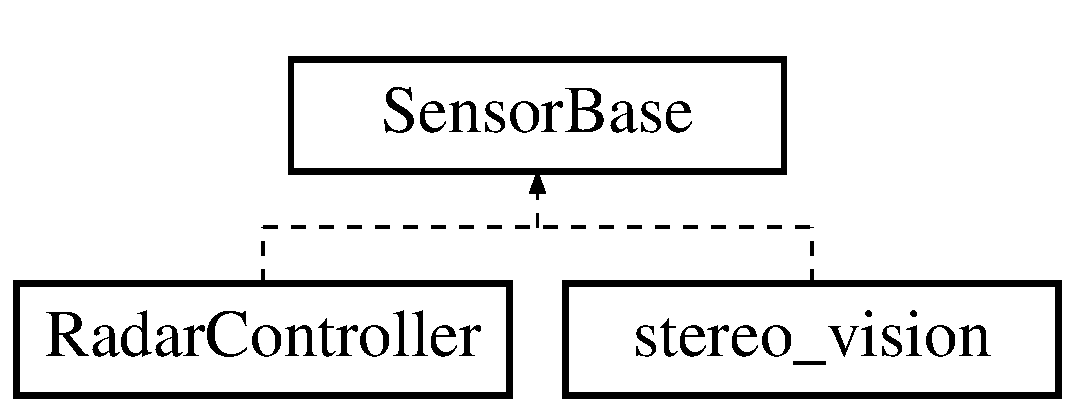
\includegraphics[height=2.000000cm]{class_sensor_base}
\end{center}
\end{figure}
\subsection*{Classes}
\begin{DoxyCompactItemize}
\item 
struct \hyperlink{struct_sensor_base_1_1_p_c}{P\+C}
\end{DoxyCompactItemize}
\subsection*{Static Public Member Functions}
\begin{DoxyCompactItemize}
\item 
static cv\+::\+Point2d \hyperlink{class_sensor_base_a9ea2144c7cda85295ba3f8697354a77c}{polar2\+Cartf} (\hyperlink{struct_sensor_base_1_1_p_c}{P\+C} pc\+\_\+in, int unit\+\_\+in)
\begin{DoxyCompactList}\small\item\em polar2\+Cartf location from polar coordinate to Cartesian one \end{DoxyCompactList}\item 
static cv\+::\+Point \hyperlink{class_sensor_base_ab193b852242bb8b85976664518732dfb}{polar2\+Cart} (\hyperlink{struct_sensor_base_1_1_p_c}{P\+C} pc\+\_\+in, int unit\+\_\+in)
\begin{DoxyCompactList}\small\item\em polar2\+Cart is the same as \hyperlink{class_sensor_base_a9ea2144c7cda85295ba3f8697354a77c}{but diff. in return type }\end{DoxyCompactList}\item 
\hypertarget{class_sensor_base_afb3be773547689c4bad57a3847db7e88}{}static \hyperlink{struct_sensor_base_1_1_p_c}{Sensor\+Base\+::\+P\+C} {\bfseries cart2\+Polarf} (cv\+::\+Point2f pt\+\_\+in, int unit)\label{class_sensor_base_afb3be773547689c4bad57a3847db7e88}

\item 
\hypertarget{class_sensor_base_a7a263dfc99be499f8383a64166e6e7f8}{}static \hyperlink{struct_sensor_base_1_1_p_c}{P\+C} {\bfseries cart2\+Polar} (cv\+::\+Point pt\+\_\+in, int unit)\label{class_sensor_base_a7a263dfc99be499f8383a64166e6e7f8}

\item 
static cv\+::\+Point2f \hyperlink{class_sensor_base_acdc1ebb9c7051050bb887118e354b69f}{vel\+Unit\+Transform} (cv\+::\+Point2f src, int type)
\begin{DoxyCompactList}\small\item\em vel\+Unit\+Transform to transform velocity unit \end{DoxyCompactList}\item 
static cv\+::\+Point2f \hyperlink{class_sensor_base_a462a999b17c0217e53fcd7014d271625}{vel\+Estimation} (cv\+::\+Point2f p\+\_\+now, cv\+::\+Point2f p\+\_\+prev, float time\+\_\+proc, int type)
\begin{DoxyCompactList}\small\item\em vel\+Estimation to estimate object\textquotesingle{}s velocity \end{DoxyCompactList}\end{DoxyCompactItemize}


\subsection{Member Function Documentation}
\hypertarget{class_sensor_base_ab193b852242bb8b85976664518732dfb}{}\index{Sensor\+Base@{Sensor\+Base}!polar2\+Cart@{polar2\+Cart}}
\index{polar2\+Cart@{polar2\+Cart}!Sensor\+Base@{Sensor\+Base}}
\subsubsection[{polar2\+Cart}]{\setlength{\rightskip}{0pt plus 5cm}cv\+::\+Point Sensor\+Base\+::polar2\+Cart (
\begin{DoxyParamCaption}
\item[{{\bf Sensor\+Base\+::\+P\+C}}]{pc\+\_\+in, }
\item[{int}]{unit\+\_\+in}
\end{DoxyParamCaption}
)\hspace{0.3cm}{\ttfamily [static]}}\label{class_sensor_base_ab193b852242bb8b85976664518732dfb}


polar2\+Cart is the same as \hyperlink{class_sensor_base_a9ea2144c7cda85295ba3f8697354a77c}{but diff. in return type }


\begin{DoxyParams}{Parameters}
{\em pc\+\_\+in} & \\
\hline
{\em unit\+\_\+in} & \\
\hline
\end{DoxyParams}
\begin{DoxyReturn}{Returns}
cv\+::\+Point 
\end{DoxyReturn}
\hypertarget{class_sensor_base_a9ea2144c7cda85295ba3f8697354a77c}{}\index{Sensor\+Base@{Sensor\+Base}!polar2\+Cartf@{polar2\+Cartf}}
\index{polar2\+Cartf@{polar2\+Cartf}!Sensor\+Base@{Sensor\+Base}}
\subsubsection[{polar2\+Cartf}]{\setlength{\rightskip}{0pt plus 5cm}cv\+::\+Point2d Sensor\+Base\+::polar2\+Cartf (
\begin{DoxyParamCaption}
\item[{{\bf Sensor\+Base\+::\+P\+C}}]{pc\+\_\+in, }
\item[{int}]{unit\+\_\+in}
\end{DoxyParamCaption}
)\hspace{0.3cm}{\ttfamily [static]}}\label{class_sensor_base_a9ea2144c7cda85295ba3f8697354a77c}


polar2\+Cartf location from polar coordinate to Cartesian one 


\begin{DoxyParams}{Parameters}
{\em pc\+\_\+in} & \\
\hline
{\em unit\+\_\+in} & \\
\hline
\end{DoxyParams}
\begin{DoxyReturn}{Returns}
cv\+::\+Point2d 
\end{DoxyReturn}
\hypertarget{class_sensor_base_a462a999b17c0217e53fcd7014d271625}{}\index{Sensor\+Base@{Sensor\+Base}!vel\+Estimation@{vel\+Estimation}}
\index{vel\+Estimation@{vel\+Estimation}!Sensor\+Base@{Sensor\+Base}}
\subsubsection[{vel\+Estimation}]{\setlength{\rightskip}{0pt plus 5cm}cv\+::\+Point2f Sensor\+Base\+::vel\+Estimation (
\begin{DoxyParamCaption}
\item[{cv\+::\+Point2f}]{p\+\_\+now, }
\item[{cv\+::\+Point2f}]{p\+\_\+prev, }
\item[{float}]{time\+\_\+proc, }
\item[{int}]{type}
\end{DoxyParamCaption}
)\hspace{0.3cm}{\ttfamily [static]}}\label{class_sensor_base_a462a999b17c0217e53fcd7014d271625}


vel\+Estimation to estimate object\textquotesingle{}s velocity 


\begin{DoxyParams}{Parameters}
{\em p\+\_\+now} & \\
\hline
{\em p\+\_\+prev} & \\
\hline
{\em time\+\_\+proc} & \\
\hline
{\em type} & \\
\hline
\end{DoxyParams}
\begin{DoxyReturn}{Returns}

\end{DoxyReturn}
\hypertarget{class_sensor_base_acdc1ebb9c7051050bb887118e354b69f}{}\index{Sensor\+Base@{Sensor\+Base}!vel\+Unit\+Transform@{vel\+Unit\+Transform}}
\index{vel\+Unit\+Transform@{vel\+Unit\+Transform}!Sensor\+Base@{Sensor\+Base}}
\subsubsection[{vel\+Unit\+Transform}]{\setlength{\rightskip}{0pt plus 5cm}cv\+::\+Point2f Sensor\+Base\+::vel\+Unit\+Transform (
\begin{DoxyParamCaption}
\item[{cv\+::\+Point2f}]{src, }
\item[{int}]{type}
\end{DoxyParamCaption}
)\hspace{0.3cm}{\ttfamily [static]}}\label{class_sensor_base_acdc1ebb9c7051050bb887118e354b69f}


vel\+Unit\+Transform to transform velocity unit 


\begin{DoxyParams}{Parameters}
{\em src} & velocity \\
\hline
{\em type} & like km/hr $<$-\/$>$ m/s \\
\hline
\end{DoxyParams}
\begin{DoxyReturn}{Returns}

\end{DoxyReturn}


The documentation for this class was generated from the following files\+:\begin{DoxyCompactItemize}
\item 
D\+:/\+Qt\+Program/\+Qt5/\+Fusion/sensorbase.\+h\item 
D\+:/\+Qt\+Program/\+Qt5/\+Fusion/sensorbase.\+cpp\end{DoxyCompactItemize}

\hypertarget{class_sensor_info}{}\section{Sensor\+Info Class Reference}
\label{class_sensor_info}\index{Sensor\+Info@{Sensor\+Info}}


This class deals with all the sensors\textquotesingle{} information and the fused result.  




{\ttfamily \#include $<$sensorinfo.\+h$>$}

Inheritance diagram for Sensor\+Info\+:\begin{figure}[H]
\begin{center}
\leavevmode
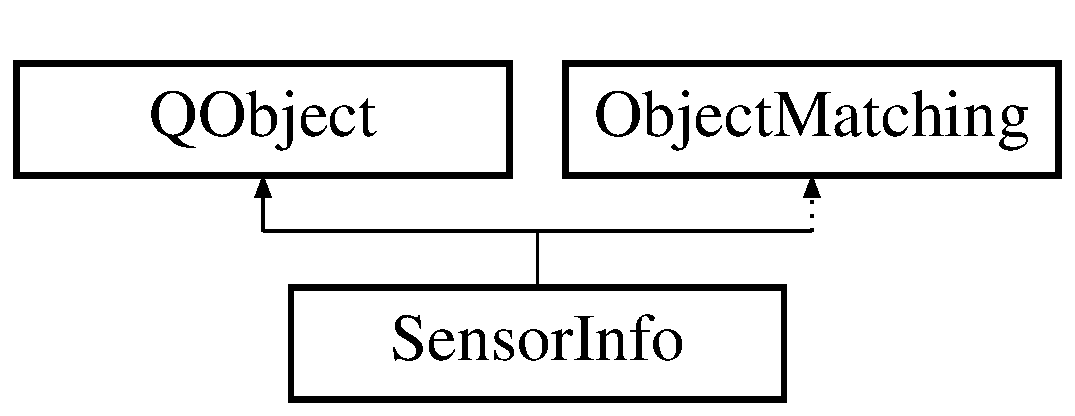
\includegraphics[height=2.000000cm]{class_sensor_info}
\end{center}
\end{figure}
\subsection*{Classes}
\begin{DoxyCompactItemize}
\item 
struct \hyperlink{struct_sensor_info_1_1sensor_information}{sensor\+Information}
\begin{DoxyCompactList}\small\item\em The \hyperlink{struct_sensor_info_1_1sensor_information}{sensor\+Information} struct is the information of objects detected by different sensors. Based on fused topview. \end{DoxyCompactList}\item 
struct \hyperlink{struct_sensor_info_1_1sensor_location}{sensor\+Location}
\begin{DoxyCompactList}\small\item\em $<$ sensor location \end{DoxyCompactList}\item 
struct \hyperlink{struct_sensor_info_1_1vehicle_info}{vehicle\+Info}
\begin{DoxyCompactList}\small\item\em The \hyperlink{struct_sensor_info_1_1vehicle_info}{vehicle\+Info} struct to save the vehicle\textquotesingle{}s basic info. \end{DoxyCompactList}\end{DoxyCompactItemize}
\subsection*{Signals}
\begin{DoxyCompactItemize}
\item 
\hypertarget{class_sensor_info_a4319ce78ed6efa273de1353d7dc687ae}{}void {\bfseries update\+G\+U\+I} (cv\+::\+Mat $\ast$\hyperlink{class_sensor_info_a8862f0f8415919416a94165f31542222}{fused\+\_\+topview}, cv\+::\+Mat $\ast$img\+\_\+detected\+\_\+display)\label{class_sensor_info_a4319ce78ed6efa273de1353d7dc687ae}

\item 
\hypertarget{class_sensor_info_a41a6018d7dfa24a65dfa3510c730765c}{}void {\bfseries gui\+Display} (int type, bool fg\+\_\+on)\label{class_sensor_info_a41a6018d7dfa24a65dfa3510c730765c}

\end{DoxyCompactItemize}
\subsection*{Public Member Functions}
\begin{DoxyCompactItemize}
\item 
\hypertarget{class_sensor_info_a5cf4cd38a1a4779612aa15b78a516b20}{}void \hyperlink{class_sensor_info_a5cf4cd38a1a4779612aa15b78a516b20}{reset\+Tracking\+Info} ()\label{class_sensor_info_a5cf4cd38a1a4779612aa15b78a516b20}

\begin{DoxyCompactList}\small\item\em clear std\+::vector$<$object\+Tracking$>$ ti \end{DoxyCompactList}\item 
int \hyperlink{class_sensor_info_ad3aceaec34ba17e59bebc8c37679e4d7}{sv\+Data\+Exec} ()
\begin{DoxyCompactList}\small\item\em Retrieving data from stereo vision. \end{DoxyCompactList}\item 
int \hyperlink{class_sensor_info_aba48141526605d2b9a39585b1221293d}{radar\+Data\+Exec} ()
\begin{DoxyCompactList}\small\item\em Retrieving data from radar. \end{DoxyCompactList}\item 
bool \hyperlink{class_sensor_info_abc177db051acc8cec5e06261042baa3a}{lrf\+Data\+Exec} ()
\begin{DoxyCompactList}\small\item\em Retrieving data from laser rangefinder. \end{DoxyCompactList}\item 
\hypertarget{class_sensor_info_a7ad4246a8f17cee7e95dc9e3f2762e15}{}void \hyperlink{class_sensor_info_a7ad4246a8f17cee7e95dc9e3f2762e15}{lrf\+Buf\+Exec} ()\label{class_sensor_info_a7ad4246a8f17cee7e95dc9e3f2762e15}

\begin{DoxyCompactList}\small\item\em Retrieving lrf data to buf. \end{DoxyCompactList}\item 
void \hyperlink{class_sensor_info_adf375036103c9b7e3a3bf10b472ca6be}{choose\+Vehicle} (int vehicle\+\_\+type)
\begin{DoxyCompactList}\small\item\em choose\+Vehicle to modify topview\textquotesingle{}s setting with different vehicles \end{DoxyCompactList}\item 
void \hyperlink{class_sensor_info_aa8031ea5907d5822d21d964044ac6f11}{initial\+Fused\+Top\+View} (int range\+\_\+pixel)
\begin{DoxyCompactList}\small\item\em initial\+Fused\+Top\+View \end{DoxyCompactList}\item 
\hypertarget{class_sensor_info_a949ffd6e8141a1ea36a81daf18773bbe}{}void \hyperlink{class_sensor_info_a949ffd6e8141a1ea36a81daf18773bbe}{update\+Fused\+Top\+View} ()\label{class_sensor_info_a949ffd6e8141a1ea36a81daf18773bbe}

\begin{DoxyCompactList}\small\item\em update\+Fused\+Top\+View Update the fused topview w/ different detection range \end{DoxyCompactList}\item 
void \hyperlink{class_sensor_info_a84c1404a225b5795af3b8383753daf2a}{update\+Fused\+Data} ()
\begin{DoxyCompactList}\small\item\em update\+Fused\+Data Transform data from P\+C to display coordinates \end{DoxyCompactList}\item 
\hypertarget{class_sensor_info_aeeb4f996917547ec595735a593123fb2}{}void \hyperlink{class_sensor_info_aeeb4f996917547ec595735a593123fb2}{data\+Exec} ()\label{class_sensor_info_aeeb4f996917547ec595735a593123fb2}

\begin{DoxyCompactList}\small\item\em data\+Exec Fusion main function \end{DoxyCompactList}\item 
\hypertarget{class_sensor_info_abdf7ecd5f4cfdc2ebe9dadaf3723339f}{}void \hyperlink{class_sensor_info_abdf7ecd5f4cfdc2ebe9dadaf3723339f}{zoom\+Out\+Fused\+Top\+View} ()\label{class_sensor_info_abdf7ecd5f4cfdc2ebe9dadaf3723339f}

\begin{DoxyCompactList}\small\item\em zoom\+Out\+Fused\+Top\+View to zoom out the detecting range of fused topview \end{DoxyCompactList}\item 
\hypertarget{class_sensor_info_a1bf4f300f920de29385b5747e1e5759f}{}void \hyperlink{class_sensor_info_a1bf4f300f920de29385b5747e1e5759f}{zoom\+In\+Fused\+Top\+View} ()\label{class_sensor_info_a1bf4f300f920de29385b5747e1e5759f}

\begin{DoxyCompactList}\small\item\em zoom\+In\+Fused\+Top\+View to zoom in the detecting range of fused topview \end{DoxyCompactList}\end{DoxyCompactItemize}
\subsection*{Public Attributes}
\begin{DoxyCompactItemize}
\item 
\hypertarget{class_sensor_info_a4e3f1250f396a7229a9d2195429ab95c}{}\hyperlink{classstereo__vision}{stereo\+\_\+vision} $\ast$ \hyperlink{class_sensor_info_a4e3f1250f396a7229a9d2195429ab95c}{sv}\label{class_sensor_info_a4e3f1250f396a7229a9d2195429ab95c}

\begin{DoxyCompactList}\small\item\em pointer of class \hyperlink{classstereo__vision}{stereo\+\_\+vision} \end{DoxyCompactList}\item 
\hypertarget{class_sensor_info_a3138edb6c3a02a2c0b31a3f70afa74ba}{}\hyperlink{class_radar_controller}{Radar\+Controller} $\ast$ \hyperlink{class_sensor_info_a3138edb6c3a02a2c0b31a3f70afa74ba}{rc}\label{class_sensor_info_a3138edb6c3a02a2c0b31a3f70afa74ba}

\begin{DoxyCompactList}\small\item\em pointer of class \hyperlink{class_radar_controller}{Radar\+Controller} \end{DoxyCompactList}\item 
\hypertarget{class_sensor_info_a237508ffb14be65b71a5578da5f4e01c}{}\hyperlink{classlrf__controller}{lrf\+\_\+controller} $\ast$ \hyperlink{class_sensor_info_a237508ffb14be65b71a5578da5f4e01c}{lrf}\label{class_sensor_info_a237508ffb14be65b71a5578da5f4e01c}

\begin{DoxyCompactList}\small\item\em pointer of class \hyperlink{classlrf__controller}{lrf\+\_\+controller} \end{DoxyCompactList}\item 
\hypertarget{class_sensor_info_a75484cb15fb13e0ce29c0e9dd99d2c2b}{}Object\+Tracking\+::object\+Tracking\+Info $\ast$ \hyperlink{class_sensor_info_a75484cb15fb13e0ce29c0e9dd99d2c2b}{data\+\_\+fused}\label{class_sensor_info_a75484cb15fb13e0ce29c0e9dd99d2c2b}

\begin{DoxyCompactList}\small\item\em fused information (single) \end{DoxyCompactList}\item 
\hypertarget{class_sensor_info_aec5c17cd1b09659a924021bb58826192}{}Object\+Tracking $\ast$ \hyperlink{class_sensor_info_aec5c17cd1b09659a924021bb58826192}{ot\+\_\+fused}\label{class_sensor_info_aec5c17cd1b09659a924021bb58826192}

\begin{DoxyCompactList}\small\item\em tracking fused data (continuous) \end{DoxyCompactList}\item 
\hypertarget{class_sensor_info_af9aa110890f48a9bd2cd44e960c3ef60}{}Collision\+Avoidance $\ast$ \hyperlink{class_sensor_info_af9aa110890f48a9bd2cd44e960c3ef60}{ca}\label{class_sensor_info_af9aa110890f48a9bd2cd44e960c3ef60}

\begin{DoxyCompactList}\small\item\em pointer of class Collision\+Avoidance \end{DoxyCompactList}\item 
\hypertarget{class_sensor_info_a1970954c71534f432c13165864a3efca}{}bool \hyperlink{class_sensor_info_a1970954c71534f432c13165864a3efca}{fg\+\_\+proc}\label{class_sensor_info_a1970954c71534f432c13165864a3efca}

\begin{DoxyCompactList}\small\item\em wether fusion function is processing \end{DoxyCompactList}\item 
\hypertarget{class_sensor_info_a207a7b13dd2fe49ca4a5cd7f5c183004}{}bool \hyperlink{class_sensor_info_a207a7b13dd2fe49ca4a5cd7f5c183004}{fg\+\_\+sv}\label{class_sensor_info_a207a7b13dd2fe49ca4a5cd7f5c183004}

\begin{DoxyCompactList}\small\item\em check if the sv is processing and need to be processed in fusion function \end{DoxyCompactList}\item 
\hypertarget{class_sensor_info_af0b67a69fa0c2d346b8f0e4b72f7d84f}{}bool \hyperlink{class_sensor_info_af0b67a69fa0c2d346b8f0e4b72f7d84f}{fg\+\_\+sv\+\_\+each\+\_\+pixel}\label{class_sensor_info_af0b67a69fa0c2d346b8f0e4b72f7d84f}

\begin{DoxyCompactList}\small\item\em plot all the pixel information in the fused topview or not \end{DoxyCompactList}\item 
\hypertarget{class_sensor_info_aa526e31c8b20b439088564a9b2bb86e9}{}bool \hyperlink{class_sensor_info_aa526e31c8b20b439088564a9b2bb86e9}{fg\+\_\+radar}\label{class_sensor_info_aa526e31c8b20b439088564a9b2bb86e9}

\begin{DoxyCompactList}\small\item\em check if the radar is processing and need to be processed in fusion function \end{DoxyCompactList}\item 
\hypertarget{class_sensor_info_a20a40d7fe32d657e543cc241c6aa98ab}{}bool \hyperlink{class_sensor_info_a20a40d7fe32d657e543cc241c6aa98ab}{fg\+\_\+data\+\_\+update}\label{class_sensor_info_a20a40d7fe32d657e543cc241c6aa98ab}

\begin{DoxyCompactList}\small\item\em check status of sensors is processing or not \end{DoxyCompactList}\item 
\hypertarget{class_sensor_info_a231c2936351dc2325334f0988bde478c}{}bool \hyperlink{class_sensor_info_a231c2936351dc2325334f0988bde478c}{fg\+\_\+fusion}\label{class_sensor_info_a231c2936351dc2325334f0988bde478c}

\begin{DoxyCompactList}\small\item\em check for run fusion function \end{DoxyCompactList}\item 
\hypertarget{class_sensor_info_aeed9690aa611953f6ea450c63767b138}{}bool \hyperlink{class_sensor_info_aeed9690aa611953f6ea450c63767b138}{fg\+\_\+ot}\label{class_sensor_info_aeed9690aa611953f6ea450c63767b138}

\begin{DoxyCompactList}\small\item\em check for object tracking \end{DoxyCompactList}\item 
\hypertarget{class_sensor_info_a9317c7c2d9e06d47ba292e7784fd2b2d}{}bool \hyperlink{class_sensor_info_a9317c7c2d9e06d47ba292e7784fd2b2d}{fg\+\_\+ot\+\_\+trajectory}\label{class_sensor_info_a9317c7c2d9e06d47ba292e7784fd2b2d}

\begin{DoxyCompactList}\small\item\em check for displaying trajectory on fused topview or not \end{DoxyCompactList}\item 
\hypertarget{class_sensor_info_a4ce1e5a2e2568e32c48f3a8aaddd298c}{}bool \hyperlink{class_sensor_info_a4ce1e5a2e2568e32c48f3a8aaddd298c}{fg\+\_\+ot\+\_\+trajectory\+\_\+raw}\label{class_sensor_info_a4ce1e5a2e2568e32c48f3a8aaddd298c}

\begin{DoxyCompactList}\small\item\em check for displaying raw traj. \end{DoxyCompactList}\item 
\hypertarget{class_sensor_info_a72d293d7c4f782bda708990a24e33cd4}{}bool \hyperlink{class_sensor_info_a72d293d7c4f782bda708990a24e33cd4}{fg\+\_\+ot\+\_\+trajectory\+\_\+kalman}\label{class_sensor_info_a72d293d7c4f782bda708990a24e33cd4}

\begin{DoxyCompactList}\small\item\em check for displaying Kalman filtered traj. \end{DoxyCompactList}\item 
\hypertarget{class_sensor_info_a81403b882ea7e5fec8aa58e7432f0b24}{}bool \hyperlink{class_sensor_info_a81403b882ea7e5fec8aa58e7432f0b24}{fg\+\_\+ot\+\_\+vel}\label{class_sensor_info_a81403b882ea7e5fec8aa58e7432f0b24}

\begin{DoxyCompactList}\small\item\em check for displaying velocity \end{DoxyCompactList}\item 
\hypertarget{class_sensor_info_a8d65786045ff99eddfc80f8db962e19d}{}bool \hyperlink{class_sensor_info_a8d65786045ff99eddfc80f8db962e19d}{fg\+\_\+ot\+\_\+kf}\label{class_sensor_info_a8d65786045ff99eddfc80f8db962e19d}

\begin{DoxyCompactList}\small\item\em check for running Kalaman filter \end{DoxyCompactList}\item 
\hypertarget{class_sensor_info_a11d1247334e1bbb62a0fd8eca9c6addc}{}bool \hyperlink{class_sensor_info_a11d1247334e1bbb62a0fd8eca9c6addc}{fg\+\_\+ot\+\_\+pf}\label{class_sensor_info_a11d1247334e1bbb62a0fd8eca9c6addc}

\begin{DoxyCompactList}\small\item\em \mbox{[}unused\mbox{]} for running particle filter \end{DoxyCompactList}\item 
\hypertarget{class_sensor_info_ac5aae66f8cbfb76ef869f1b474c64707}{}bool \hyperlink{class_sensor_info_ac5aae66f8cbfb76ef869f1b474c64707}{fg\+\_\+ca\+\_\+astar}\label{class_sensor_info_ac5aae66f8cbfb76ef869f1b474c64707}

\begin{DoxyCompactList}\small\item\em check for running A$\ast$ algo. \end{DoxyCompactList}\item 
\hypertarget{class_sensor_info_a52869f08515c02e4ad3e1b1c8f07577e}{}bool \hyperlink{class_sensor_info_a52869f08515c02e4ad3e1b1c8f07577e}{fg\+\_\+ca\+\_\+vfh}\label{class_sensor_info_a52869f08515c02e4ad3e1b1c8f07577e}

\begin{DoxyCompactList}\small\item\em check for running V\+F\+H algo. \end{DoxyCompactList}\item 
\hypertarget{class_sensor_info_ac8296477bcba77644ce34fac1b7087a9}{}bool \hyperlink{class_sensor_info_ac8296477bcba77644ce34fac1b7087a9}{fg\+\_\+fused\+\_\+region\+\_\+display\+\_\+only}\label{class_sensor_info_ac8296477bcba77644ce34fac1b7087a9}

\begin{DoxyCompactList}\small\item\em check for displaying only sensors\textquotesingle{} overlapped region \end{DoxyCompactList}\item 
\hypertarget{class_sensor_info_acb3b875ad574515cbb67c06a23fc74c1}{}bool \hyperlink{class_sensor_info_acb3b875ad574515cbb67c06a23fc74c1}{fg\+\_\+display\+\_\+literature\+\_\+mode}\label{class_sensor_info_acb3b875ad574515cbb67c06a23fc74c1}

\begin{DoxyCompactList}\small\item\em displaying mode change button \end{DoxyCompactList}\item 
\hypertarget{class_sensor_info_a1b395f161a1e8fa5562f4e48f0ca2865}{}Q\+Pixmap \hyperlink{class_sensor_info_a1b395f161a1e8fa5562f4e48f0ca2865}{pic\+\_\+sv}\label{class_sensor_info_a1b395f161a1e8fa5562f4e48f0ca2865}

\begin{DoxyCompactList}\small\item\em display color of S\+V sensor \end{DoxyCompactList}\item 
\hypertarget{class_sensor_info_a528cfd0ab5a94093f2e3767ea765c988}{}Q\+Pixmap \hyperlink{class_sensor_info_a528cfd0ab5a94093f2e3767ea765c988}{pic\+\_\+radar}\label{class_sensor_info_a528cfd0ab5a94093f2e3767ea765c988}

\begin{DoxyCompactList}\small\item\em display color of R\+A\+D\+A\+R sensor \end{DoxyCompactList}\item 
\hypertarget{class_sensor_info_a23eb32e568652541c7aa6b32097f43b8}{}cv\+::\+Mat \hyperlink{class_sensor_info_a23eb32e568652541c7aa6b32097f43b8}{fused\+\_\+topview\+\_\+\+B\+G}\label{class_sensor_info_a23eb32e568652541c7aa6b32097f43b8}

\begin{DoxyCompactList}\small\item\em background of fused topview \end{DoxyCompactList}\item 
\hypertarget{class_sensor_info_a8862f0f8415919416a94165f31542222}{}cv\+::\+Mat \hyperlink{class_sensor_info_a8862f0f8415919416a94165f31542222}{fused\+\_\+topview}\label{class_sensor_info_a8862f0f8415919416a94165f31542222}

\begin{DoxyCompactList}\small\item\em foreground of fused topview \end{DoxyCompactList}\end{DoxyCompactItemize}
\subsection*{Private Types}
\begin{DoxyCompactItemize}
\item 
enum \{ \hyperlink{class_sensor_info_a1507edd91570cb8c0d44ccd944c41d4ba305da288a7f76e78e827842b7fb6a1ce}{C\+T\+\_\+\+W\+C\+S2\+S\+C\+S}, 
\hyperlink{class_sensor_info_a1507edd91570cb8c0d44ccd944c41d4ba14fc288aa74a572019a88d1596930454}{C\+T\+\_\+\+S\+C\+S2\+W\+C\+S}
 \}
\end{DoxyCompactItemize}
\subsection*{Private Slots}
\begin{DoxyCompactItemize}
\item 
void \hyperlink{class_sensor_info_af10798b424236b1ccb456a5a0b004d38}{draw\+Arrow} (cv\+::\+Mat \&img, cv\+::\+Point p\+Start, cv\+::\+Point p\+End, int len, int alpha, cv\+::\+Scalar \&color, int \hyperlink{class_sensor_info_a6219a61c1556e2acb5d9c0a9b32f6b02}{thickness}=1, int line\+Type=8)
\begin{DoxyCompactList}\small\item\em draw\+Arrow \end{DoxyCompactList}\end{DoxyCompactItemize}
\subsection*{Private Member Functions}
\begin{DoxyCompactItemize}
\item 
void \hyperlink{class_sensor_info_a3ed48f9d9d629f385b26cc490e33950f}{reset\+Fusion} ()
\begin{DoxyCompactList}\small\item\em reset\+Fusion to reset \end{DoxyCompactList}\item 
void \hyperlink{class_sensor_info_a6b51dff8a9c8f958bd883d882afc6efb}{data\+Process} (bool \hyperlink{class_sensor_info_a207a7b13dd2fe49ca4a5cd7f5c183004}{fg\+\_\+sv}, bool \hyperlink{class_sensor_info_aa526e31c8b20b439088564a9b2bb86e9}{fg\+\_\+radar})
\begin{DoxyCompactList}\small\item\em data\+Process to fused topview and fusion information process \end{DoxyCompactList}\item 
void \hyperlink{class_sensor_info_a9916b2b7cd6af21de4ee6654be72bf6e}{reset\+Matched\+Info} (Object\+Tracking\+::object\+Tracking\+Info \&src)
\begin{DoxyCompactList}\small\item\em reset\+Matched\+Info \end{DoxyCompactList}\item 
void \hyperlink{class_sensor_info_aec57ab5b262ee80c9c257e7c216e07dc}{connect\+Matched\+Info} (Object\+Tracking\+::object\+Tracking\+Info \&src, Object\+Tracking\+::object\+Tracking\+Info \&dst)
\begin{DoxyCompactList}\small\item\em connect\+Matched\+Info to hard copy info. from src to dst and then erase src \end{DoxyCompactList}\item 
\hypertarget{class_sensor_info_ad226b2e50d1e7a871ffc43f3a28fe85a}{}void \hyperlink{class_sensor_info_ad226b2e50d1e7a871ffc43f3a28fe85a}{data\+Matching} ()\label{class_sensor_info_ad226b2e50d1e7a871ffc43f3a28fe85a}

\begin{DoxyCompactList}\small\item\em data\+Matching to match the adjacent frame object using features. Object matching\+: a) Bha. dist. of H color space, b) bias of X \& Z of W\+C\+S location Comparison of H color space image using Bhattacharyya distance with Bubble search \end{DoxyCompactList}\item 
\hypertarget{class_sensor_info_a3636d05f03ced4e9256eb9fb0fe25561}{}void \hyperlink{class_sensor_info_a3636d05f03ced4e9256eb9fb0fe25561}{data\+Tracking} ()\label{class_sensor_info_a3636d05f03ced4e9256eb9fb0fe25561}

\begin{DoxyCompactList}\small\item\em data\+Tracking to use the matching result to sotrage the object info. \end{DoxyCompactList}\item 
\hypertarget{class_sensor_info_aac27252b7430c306e78e19a617f1bc2d}{}void \hyperlink{class_sensor_info_aac27252b7430c306e78e19a617f1bc2d}{data\+Collision\+Avoidance} ()\label{class_sensor_info_aac27252b7430c306e78e19a617f1bc2d}

\begin{DoxyCompactList}\small\item\em data\+Collision\+Avoidance to do the collision avoidance \end{DoxyCompactList}\item 
void \hyperlink{class_sensor_info_ab35fa7516129114c548fcb12f37605c4}{draw\+Fused\+Top\+View} (bool \hyperlink{class_sensor_info_a207a7b13dd2fe49ca4a5cd7f5c183004}{fg\+\_\+sv}, bool \hyperlink{class_sensor_info_aa526e31c8b20b439088564a9b2bb86e9}{fg\+\_\+radar}, bool fg\+\_\+sv\+\_\+each, bool \hyperlink{class_sensor_info_a9317c7c2d9e06d47ba292e7784fd2b2d}{fg\+\_\+ot\+\_\+trajectory}, bool \hyperlink{class_sensor_info_a4ce1e5a2e2568e32c48f3a8aaddd298c}{fg\+\_\+ot\+\_\+trajectory\+\_\+raw}, bool \hyperlink{class_sensor_info_a72d293d7c4f782bda708990a24e33cd4}{fg\+\_\+ot\+\_\+trajectory\+\_\+kalman}, bool \hyperlink{class_sensor_info_a8d65786045ff99eddfc80f8db962e19d}{fg\+\_\+ot\+\_\+kf}, bool \hyperlink{class_sensor_info_ac8296477bcba77644ce34fac1b7087a9}{fg\+\_\+fused\+\_\+region\+\_\+display\+\_\+only})
\begin{DoxyCompactList}\small\item\em draw\+Fused\+Top\+View \end{DoxyCompactList}\item 
\hyperlink{struct_sensor_base_1_1_p_c}{Sensor\+Base\+::\+P\+C} \hyperlink{class_sensor_info_ac9705baab1609e71afe5b5599f2ab783}{coordinate\+Transform} (int type, cv\+::\+Point sensor\+\_\+pos, \hyperlink{struct_sensor_base_1_1_p_c}{Sensor\+Base\+::\+P\+C} pc\+\_\+in)
\begin{DoxyCompactList}\small\item\em coordinate\+Transform. The transformation of coordinates system \end{DoxyCompactList}\item 
\hypertarget{class_sensor_info_ac7b3c8df5b0b592711756d72c0f070c9}{}cv\+::\+Rect {\bfseries rect\+On\+Fused\+Top\+View} (cv\+::\+Point pt\+\_\+pixel, cv\+::\+Rect rect\+\_\+in)\label{class_sensor_info_ac7b3c8df5b0b592711756d72c0f070c9}

\item 
\hypertarget{class_sensor_info_ad1ca7e43a1110587b3bd5dfc2e456e04}{}cv\+::\+Point {\bfseries point2\+Fused\+Top\+View} (cv\+::\+Point sensor\+\_\+pos, \hyperlink{struct_sensor_base_1_1_p_c}{Sensor\+Base\+::\+P\+C} pc)\label{class_sensor_info_ad1ca7e43a1110587b3bd5dfc2e456e04}

\item 
\hypertarget{class_sensor_info_a3eaa24b9ef5c65b3ec657650c033239d}{}cv\+::\+Point {\bfseries point2\+Fused\+Top\+View} (\hyperlink{struct_sensor_base_1_1_p_c}{Sensor\+Base\+::\+P\+C} pc\+\_\+world)\label{class_sensor_info_a3eaa24b9ef5c65b3ec657650c033239d}

\item 
\hypertarget{class_sensor_info_ac8151e69e77059719163ddd0147df7c5}{}cv\+::\+Point {\bfseries point2\+Fused\+Top\+View} (cv\+::\+Point pos\+\_\+world)\label{class_sensor_info_ac8151e69e77059719163ddd0147df7c5}

\end{DoxyCompactItemize}
\subsection*{Private Attributes}
\begin{DoxyCompactItemize}
\item 
\hypertarget{class_sensor_info_acec557aa13acf29cb6592b7b0810f52f}{}Q\+Time \hyperlink{class_sensor_info_acec557aa13acf29cb6592b7b0810f52f}{t}\label{class_sensor_info_acec557aa13acf29cb6592b7b0810f52f}

\begin{DoxyCompactList}\small\item\em current thread processing time. Used for updating G\+U\+I. \end{DoxyCompactList}\item 
\hypertarget{class_sensor_info_a79e684fb00f7bde838c618836e6ef4c7}{}int \hyperlink{class_sensor_info_a79e684fb00f7bde838c618836e6ef4c7}{time\+\_\+gap}\label{class_sensor_info_a79e684fb00f7bde838c618836e6ef4c7}

\begin{DoxyCompactList}\small\item\em Threshold elapse of updating G\+U\+I. \end{DoxyCompactList}\item 
\hypertarget{class_sensor_info_aa91a3251257f08cdff5de11523bb5bff}{}int \hyperlink{class_sensor_info_aa91a3251257f08cdff5de11523bb5bff}{size\+\_\+data\+\_\+fused}\label{class_sensor_info_aa91a3251257f08cdff5de11523bb5bff}

\begin{DoxyCompactList}\small\item\em M\+A\+X sotrage amount of object. It\textquotesingle{}s the sum of obj. from S\+V and R\+A\+D\+A\+R now (2015). \end{DoxyCompactList}\item 
\hypertarget{class_sensor_info_ad9311546eadd687087567a2d836f5161}{}double \hyperlink{class_sensor_info_ad9311546eadd687087567a2d836f5161}{var\+\_\+sv} \mbox{[}2\mbox{]}\label{class_sensor_info_ad9311546eadd687087567a2d836f5161}

\begin{DoxyCompactList}\small\item\em param. of fusion function of S\+V \end{DoxyCompactList}\item 
\hypertarget{class_sensor_info_a963dbcca0e0561aa467df67b0366f409}{}double \hyperlink{class_sensor_info_a963dbcca0e0561aa467df67b0366f409}{var\+\_\+radar} \mbox{[}2\mbox{]}\label{class_sensor_info_a963dbcca0e0561aa467df67b0366f409}

\begin{DoxyCompactList}\small\item\em param. of fusion function of R\+A\+D\+A\+R \end{DoxyCompactList}\item 
\hypertarget{class_sensor_info_aa9131e08fa3152702d373e225cadea0c}{}double \hyperlink{class_sensor_info_aa9131e08fa3152702d373e225cadea0c}{var\+\_\+fused} \mbox{[}2\mbox{]}\label{class_sensor_info_aa9131e08fa3152702d373e225cadea0c}

\begin{DoxyCompactList}\small\item\em param. of fusion function \end{DoxyCompactList}\item 
\hypertarget{class_sensor_info_a7481e34fff1d337962ed74e8251db482}{}double \hyperlink{class_sensor_info_a7481e34fff1d337962ed74e8251db482}{param\+\_\+p} \mbox{[}4\mbox{]}\label{class_sensor_info_a7481e34fff1d337962ed74e8251db482}

\begin{DoxyCompactList}\small\item\em curve fitting params for fusion function \end{DoxyCompactList}\item 
\hypertarget{class_sensor_info_ac301f69f003ea6c32bf16166be172d8d}{}double \hyperlink{class_sensor_info_ac301f69f003ea6c32bf16166be172d8d}{param\+\_\+u} \mbox{[}4\mbox{]}\label{class_sensor_info_ac301f69f003ea6c32bf16166be172d8d}

\begin{DoxyCompactList}\small\item\em the same as {\ttfamily param\+\_\+p} \end{DoxyCompactList}\item 
\hypertarget{class_sensor_info_a0898d5a31aea436fc9590ef871d35dbc}{}std\+::vector$<$ int $>$ \hyperlink{class_sensor_info_a0898d5a31aea436fc9590ef871d35dbc}{cri}\label{class_sensor_info_a0898d5a31aea436fc9590ef871d35dbc}

\begin{DoxyCompactList}\small\item\em Array of closest\+\_\+radar\textquotesingle{}s id. \end{DoxyCompactList}\item 
\hypertarget{class_sensor_info_a5270ab176bd0c0b33042650729108d2a}{}double \hyperlink{class_sensor_info_a5270ab176bd0c0b33042650729108d2a}{U\+\_\+\+D}\label{class_sensor_info_a5270ab176bd0c0b33042650729108d2a}

\begin{DoxyCompactList}\small\item\em Max distance error (cm) \end{DoxyCompactList}\item 
\hypertarget{class_sensor_info_ae483e67380ee479e1dee1840644105c9}{}double \hyperlink{class_sensor_info_ae483e67380ee479e1dee1840644105c9}{R\+\_\+sv}\label{class_sensor_info_ae483e67380ee479e1dee1840644105c9}

\begin{DoxyCompactList}\small\item\em Detection radius w/ object\textquotesingle{}s S\+V center (cm) \end{DoxyCompactList}\item 
\hypertarget{class_sensor_info_a5af9d7c15dae1f54f1fc827b842179dc}{}cv\+::\+Point2d \hyperlink{class_sensor_info_a5af9d7c15dae1f54f1fc827b842179dc}{sv\+\_\+pos}\label{class_sensor_info_a5af9d7c15dae1f54f1fc827b842179dc}

\begin{DoxyCompactList}\small\item\em S\+V\textquotesingle{}s Cartesian position for fusion. \end{DoxyCompactList}\item 
\hypertarget{class_sensor_info_ab757056695c005f6e0587cd2828206af}{}\hyperlink{struct_sensor_base_1_1_p_c}{Sensor\+Base\+::\+P\+C} \hyperlink{class_sensor_info_ab757056695c005f6e0587cd2828206af}{radar\+\_\+mean}\label{class_sensor_info_ab757056695c005f6e0587cd2828206af}

\begin{DoxyCompactList}\small\item\em R\+A\+D\+A\+R\textquotesingle{}s average position if there\textquotesingle{}s more than one retrieved data while a single S\+V data retrieving. \end{DoxyCompactList}\item 
\hypertarget{class_sensor_info_ad03bdf102a3198e3d7a1e63ecc458b14}{}cv\+::\+Point \hyperlink{class_sensor_info_ad03bdf102a3198e3d7a1e63ecc458b14}{radar\+\_\+plot\+\_\+pt\+\_\+f}\label{class_sensor_info_ad03bdf102a3198e3d7a1e63ecc458b14}

\begin{DoxyCompactList}\small\item\em R\+A\+D\+A\+R\textquotesingle{}s Cartesian position for fusion. \end{DoxyCompactList}\item 
\hypertarget{class_sensor_info_a1f6c558bd14ebea1afd4340dd192c2fa}{}cv\+::\+Point2f \hyperlink{class_sensor_info_a1f6c558bd14ebea1afd4340dd192c2fa}{radar\+\_\+vel}\label{class_sensor_info_a1f6c558bd14ebea1afd4340dd192c2fa}

\begin{DoxyCompactList}\small\item\em \mbox{[}unused\mbox{]} R\+A\+D\+A\+R\textquotesingle{}s velocity \end{DoxyCompactList}\item 
\hypertarget{class_sensor_info_abf45d1d44c8c514ac08436fd3cb49e20}{}std\+::vector$<$ matched\+Result $>$ \hyperlink{class_sensor_info_abf45d1d44c8c514ac08436fd3cb49e20}{matching\+\_\+result}\label{class_sensor_info_abf45d1d44c8c514ac08436fd3cb49e20}

\begin{DoxyCompactList}\small\item\em record the result of object matching \end{DoxyCompactList}\item 
\hypertarget{class_sensor_info_a40a4baa34f55a59904e324b650a554d9}{}cv\+::\+R\+N\+G \hyperlink{class_sensor_info_a40a4baa34f55a59904e324b650a554d9}{rng}\label{class_sensor_info_a40a4baa34f55a59904e324b650a554d9}

\begin{DoxyCompactList}\small\item\em rng for traj. color \end{DoxyCompactList}\item 
\hypertarget{class_sensor_info_ae99e7853a9994afa0006104d7dffe52c}{}int \hyperlink{class_sensor_info_ae99e7853a9994afa0006104d7dffe52c}{gui\+\_\+display\+\_\+time}\label{class_sensor_info_ae99e7853a9994afa0006104d7dffe52c}

\begin{DoxyCompactList}\small\item\em current thread runtime \end{DoxyCompactList}\item 
\hypertarget{class_sensor_info_a9129c44c0a6ee9f0cae8225faad27907}{}int \hyperlink{class_sensor_info_a9129c44c0a6ee9f0cae8225faad27907}{gui\+\_\+display\+\_\+max} = 20\label{class_sensor_info_a9129c44c0a6ee9f0cae8225faad27907}

\begin{DoxyCompactList}\small\item\em threshold for updating gui of pre-\/collision warning \end{DoxyCompactList}\item 
\hypertarget{class_sensor_info_a0173834b9d6c50ab6bca8c275123ed20}{}int \hyperlink{class_sensor_info_a0173834b9d6c50ab6bca8c275123ed20}{range\+\_\+precision}\label{class_sensor_info_a0173834b9d6c50ab6bca8c275123ed20}

\begin{DoxyCompactList}\small\item\em precision of showing number on the fused topview \end{DoxyCompactList}\item 
\hypertarget{class_sensor_info_a177c1c97b1505d80645aee801e5cf34c}{}int \hyperlink{class_sensor_info_a177c1c97b1505d80645aee801e5cf34c}{detection\+\_\+range\+\_\+pixel}\label{class_sensor_info_a177c1c97b1505d80645aee801e5cf34c}

\begin{DoxyCompactList}\small\item\em fused topview radius (pixel) \end{DoxyCompactList}\item 
\hypertarget{class_sensor_info_ae385659398e7d5c3006e5c63fa3830e4}{}float \hyperlink{class_sensor_info_ae385659398e7d5c3006e5c63fa3830e4}{detection\+\_\+range}\label{class_sensor_info_ae385659398e7d5c3006e5c63fa3830e4}

\begin{DoxyCompactList}\small\item\em real detection range radius (cm) \end{DoxyCompactList}\item 
\hypertarget{class_sensor_info_a5df127ca34d022ea03d4fbc9c143b585}{}float \hyperlink{class_sensor_info_a5df127ca34d022ea03d4fbc9c143b585}{ratio}\label{class_sensor_info_a5df127ca34d022ea03d4fbc9c143b585}

\begin{DoxyCompactList}\small\item\em scaling ratio of real to fused topview (cm -\/$>$ pixel) \end{DoxyCompactList}\item 
\hypertarget{class_sensor_info_acd4a4956498a8f4ec85b9ad17c0a2f79}{}float \hyperlink{class_sensor_info_acd4a4956498a8f4ec85b9ad17c0a2f79}{max\+\_\+detection\+\_\+range}\label{class_sensor_info_acd4a4956498a8f4ec85b9ad17c0a2f79}

\begin{DoxyCompactList}\small\item\em Max detection range in all sensors (cm) \end{DoxyCompactList}\item 
\hypertarget{class_sensor_info_ae2f24601b377681e2cddd0c0c4ecb974}{}float \hyperlink{class_sensor_info_ae2f24601b377681e2cddd0c0c4ecb974}{min\+\_\+detection\+\_\+range}\label{class_sensor_info_ae2f24601b377681e2cddd0c0c4ecb974}

\begin{DoxyCompactList}\small\item\em min detection range in all sensors (cm) \end{DoxyCompactList}\item 
\hypertarget{class_sensor_info_a6219a61c1556e2acb5d9c0a9b32f6b02}{}int \hyperlink{class_sensor_info_a6219a61c1556e2acb5d9c0a9b32f6b02}{thickness}\label{class_sensor_info_a6219a61c1556e2acb5d9c0a9b32f6b02}

\begin{DoxyCompactList}\small\item\em object params on topview \end{DoxyCompactList}\item 
\hypertarget{class_sensor_info_a45c336a2e44db823f4a320d6ef2b4d52}{}int \hyperlink{class_sensor_info_a45c336a2e44db823f4a320d6ef2b4d52}{font}\label{class_sensor_info_a45c336a2e44db823f4a320d6ef2b4d52}

\begin{DoxyCompactList}\small\item\em fused topview display font \end{DoxyCompactList}\item 
\hypertarget{class_sensor_info_a2733e9cc3035fd40566808361c5a819f}{}int \hyperlink{class_sensor_info_a2733e9cc3035fd40566808361c5a819f}{font\+\_\+size}\label{class_sensor_info_a2733e9cc3035fd40566808361c5a819f}

\begin{DoxyCompactList}\small\item\em fused topview display font size \end{DoxyCompactList}\item 
\hypertarget{class_sensor_info_ad58b0cb318df92ad6d13f5797ba63628}{}int \hyperlink{class_sensor_info_ad58b0cb318df92ad6d13f5797ba63628}{font\+\_\+thickness}\label{class_sensor_info_ad58b0cb318df92ad6d13f5797ba63628}

\begin{DoxyCompactList}\small\item\em fused topview display font thickness \end{DoxyCompactList}\item 
\hypertarget{class_sensor_info_a720be10334cf4d6ebbae55f78410a311}{}\hyperlink{struct_sensor_info_1_1sensor_information}{sensor\+Information} $\ast$ \hyperlink{class_sensor_info_a720be10334cf4d6ebbae55f78410a311}{sensors}\label{class_sensor_info_a720be10334cf4d6ebbae55f78410a311}

\begin{DoxyCompactList}\small\item\em sensors\textquotesingle{} basic information \end{DoxyCompactList}\item 
\hypertarget{class_sensor_info_ac3340fdef4056a7b024fa2286abe8bca}{}struct \hyperlink{struct_sensor_info_1_1vehicle_info}{Sensor\+Info\+::vehicle\+Info} {\bfseries vehicle}\label{class_sensor_info_ac3340fdef4056a7b024fa2286abe8bca}

\item 
\hypertarget{class_sensor_info_a59fc17191072e0c3bd1ebe41b4979bd1}{}int \hyperlink{class_sensor_info_a59fc17191072e0c3bd1ebe41b4979bd1}{gap} = 500\label{class_sensor_info_a59fc17191072e0c3bd1ebe41b4979bd1}

\begin{DoxyCompactList}\small\item\em min change value for changing detection range \end{DoxyCompactList}\end{DoxyCompactItemize}


\subsection{Detailed Description}
This class deals with all the sensors\textquotesingle{} information and the fused result. 

Sensor\+Infor class

fusion function\+:~\newline
 sigma(\+S\+V, X) = p1 $\ast$ D + p2~\newline
 sigma(\+R\+A\+D\+A\+R, X) = u1 $\ast$ exp(u2 $\ast$ D)~\newline
 sigma(\+S\+V, Z) = u3 $\ast$ exp(u4 $\ast$ D)~\newline
 sigma(\+R\+A\+D\+A\+R,\+Z) = p3 $\ast$ D + p4 

\subsection{Member Enumeration Documentation}
\hypertarget{class_sensor_info_a1507edd91570cb8c0d44ccd944c41d4b}{}\subsubsection[{anonymous enum}]{\setlength{\rightskip}{0pt plus 5cm}anonymous enum\hspace{0.3cm}{\ttfamily [private]}}\label{class_sensor_info_a1507edd91570cb8c0d44ccd944c41d4b}
Coordinate transformation used in \hyperlink{class_sensor_info_ac9705baab1609e71afe5b5599f2ab783}{coordinate\+Transform}\begin{Desc}
\item[Enumerator]\par
\begin{description}
\index{C\+T\+\_\+\+W\+C\+S2\+S\+C\+S@{C\+T\+\_\+\+W\+C\+S2\+S\+C\+S}!Sensor\+Info@{Sensor\+Info}}\index{Sensor\+Info@{Sensor\+Info}!C\+T\+\_\+\+W\+C\+S2\+S\+C\+S@{C\+T\+\_\+\+W\+C\+S2\+S\+C\+S}}\item[{\em 
\hypertarget{class_sensor_info_a1507edd91570cb8c0d44ccd944c41d4ba305da288a7f76e78e827842b7fb6a1ce}{}C\+T\+\_\+\+W\+C\+S2\+S\+C\+S\label{class_sensor_info_a1507edd91570cb8c0d44ccd944c41d4ba305da288a7f76e78e827842b7fb6a1ce}
}]from world coordinate sys. to sensor coordinate sys. \index{C\+T\+\_\+\+S\+C\+S2\+W\+C\+S@{C\+T\+\_\+\+S\+C\+S2\+W\+C\+S}!Sensor\+Info@{Sensor\+Info}}\index{Sensor\+Info@{Sensor\+Info}!C\+T\+\_\+\+S\+C\+S2\+W\+C\+S@{C\+T\+\_\+\+S\+C\+S2\+W\+C\+S}}\item[{\em 
\hypertarget{class_sensor_info_a1507edd91570cb8c0d44ccd944c41d4ba14fc288aa74a572019a88d1596930454}{}C\+T\+\_\+\+S\+C\+S2\+W\+C\+S\label{class_sensor_info_a1507edd91570cb8c0d44ccd944c41d4ba14fc288aa74a572019a88d1596930454}
}]from world coor. sys. to sensor coor. sys. \end{description}
\end{Desc}


\subsection{Member Function Documentation}
\hypertarget{class_sensor_info_adf375036103c9b7e3a3bf10b472ca6be}{}\index{Sensor\+Info@{Sensor\+Info}!choose\+Vehicle@{choose\+Vehicle}}
\index{choose\+Vehicle@{choose\+Vehicle}!Sensor\+Info@{Sensor\+Info}}
\subsubsection[{choose\+Vehicle}]{\setlength{\rightskip}{0pt plus 5cm}void Sensor\+Info\+::choose\+Vehicle (
\begin{DoxyParamCaption}
\item[{int}]{vehicle\+\_\+type}
\end{DoxyParamCaption}
)}\label{class_sensor_info_adf375036103c9b7e3a3bf10b472ca6be}


choose\+Vehicle to modify topview\textquotesingle{}s setting with different vehicles 


\begin{DoxyParams}{Parameters}
{\em vehicle\+\_\+type} & vehicle, tractor and cart. \\
\hline
\end{DoxyParams}
\hypertarget{class_sensor_info_aec57ab5b262ee80c9c257e7c216e07dc}{}\index{Sensor\+Info@{Sensor\+Info}!connect\+Matched\+Info@{connect\+Matched\+Info}}
\index{connect\+Matched\+Info@{connect\+Matched\+Info}!Sensor\+Info@{Sensor\+Info}}
\subsubsection[{connect\+Matched\+Info}]{\setlength{\rightskip}{0pt plus 5cm}void Sensor\+Info\+::connect\+Matched\+Info (
\begin{DoxyParamCaption}
\item[{Object\+Tracking\+::object\+Tracking\+Info \&}]{src, }
\item[{Object\+Tracking\+::object\+Tracking\+Info \&}]{dst}
\end{DoxyParamCaption}
)\hspace{0.3cm}{\ttfamily [private]}}\label{class_sensor_info_aec57ab5b262ee80c9c257e7c216e07dc}


connect\+Matched\+Info to hard copy info. from src to dst and then erase src 


\begin{DoxyParams}{Parameters}
{\em src} & \\
\hline
{\em dst} & \\
\hline
\end{DoxyParams}
\hypertarget{class_sensor_info_ac9705baab1609e71afe5b5599f2ab783}{}\index{Sensor\+Info@{Sensor\+Info}!coordinate\+Transform@{coordinate\+Transform}}
\index{coordinate\+Transform@{coordinate\+Transform}!Sensor\+Info@{Sensor\+Info}}
\subsubsection[{coordinate\+Transform}]{\setlength{\rightskip}{0pt plus 5cm}{\bf Sensor\+Base\+::\+P\+C} Sensor\+Info\+::coordinate\+Transform (
\begin{DoxyParamCaption}
\item[{int}]{type, }
\item[{cv\+::\+Point}]{sensor\+\_\+pos, }
\item[{{\bf Sensor\+Base\+::\+P\+C}}]{pc\+\_\+in}
\end{DoxyParamCaption}
)\hspace{0.3cm}{\ttfamily [private]}}\label{class_sensor_info_ac9705baab1609e71afe5b5599f2ab783}


coordinate\+Transform. The transformation of coordinates system 


\begin{DoxyParams}{Parameters}
{\em int} & type \\
\hline
{\em cv\+::\+Point} & sensor\+\_\+pos \\
\hline
{\em \hyperlink{struct_sensor_base_1_1_p_c}{Sensor\+Base\+::\+P\+C}} & pc\+\_\+in \\
\hline
\end{DoxyParams}
\begin{DoxyReturn}{Returns}
\hyperlink{struct_sensor_base_1_1_p_c}{Sensor\+Base\+::\+P\+C} pc\+\_\+out 
\end{DoxyReturn}
\hypertarget{class_sensor_info_a6b51dff8a9c8f958bd883d882afc6efb}{}\index{Sensor\+Info@{Sensor\+Info}!data\+Process@{data\+Process}}
\index{data\+Process@{data\+Process}!Sensor\+Info@{Sensor\+Info}}
\subsubsection[{data\+Process}]{\setlength{\rightskip}{0pt plus 5cm}void Sensor\+Info\+::data\+Process (
\begin{DoxyParamCaption}
\item[{bool}]{fg\+\_\+sv, }
\item[{bool}]{fg\+\_\+radar}
\end{DoxyParamCaption}
)\hspace{0.3cm}{\ttfamily [private]}}\label{class_sensor_info_a6b51dff8a9c8f958bd883d882afc6efb}


data\+Process to fused topview and fusion information process 


\begin{DoxyParams}{Parameters}
{\em fg\+\_\+sv} & \\
\hline
{\em fg\+\_\+radar} & \\
\hline
\end{DoxyParams}
\hypertarget{class_sensor_info_af10798b424236b1ccb456a5a0b004d38}{}\index{Sensor\+Info@{Sensor\+Info}!draw\+Arrow@{draw\+Arrow}}
\index{draw\+Arrow@{draw\+Arrow}!Sensor\+Info@{Sensor\+Info}}
\subsubsection[{draw\+Arrow}]{\setlength{\rightskip}{0pt plus 5cm}void Sensor\+Info\+::draw\+Arrow (
\begin{DoxyParamCaption}
\item[{cv\+::\+Mat \&}]{img, }
\item[{cv\+::\+Point}]{p\+Start, }
\item[{cv\+::\+Point}]{p\+End, }
\item[{int}]{len, }
\item[{int}]{alpha, }
\item[{cv\+::\+Scalar \&}]{color, }
\item[{int}]{thickness = {\ttfamily 1}, }
\item[{int}]{line\+Type = {\ttfamily 8}}
\end{DoxyParamCaption}
)\hspace{0.3cm}{\ttfamily [private]}, {\ttfamily [slot]}}\label{class_sensor_info_af10798b424236b1ccb456a5a0b004d38}


draw\+Arrow 


\begin{DoxyParams}{Parameters}
{\em img} & \\
\hline
{\em p\+Start} & arrow\textquotesingle{}s bottom \\
\hline
{\em p\+End} & arrow\textquotesingle{}s head \\
\hline
{\em len} & branch\textquotesingle{}s length \\
\hline
{\em alpha} & angle between main and branch \\
\hline
{\em color} & \\
\hline
{\em thickness} & arrow\textquotesingle{}s thickness \\
\hline
{\em line\+Type} & \\
\hline
\end{DoxyParams}
\hypertarget{class_sensor_info_ab35fa7516129114c548fcb12f37605c4}{}\index{Sensor\+Info@{Sensor\+Info}!draw\+Fused\+Top\+View@{draw\+Fused\+Top\+View}}
\index{draw\+Fused\+Top\+View@{draw\+Fused\+Top\+View}!Sensor\+Info@{Sensor\+Info}}
\subsubsection[{draw\+Fused\+Top\+View}]{\setlength{\rightskip}{0pt plus 5cm}void Sensor\+Info\+::draw\+Fused\+Top\+View (
\begin{DoxyParamCaption}
\item[{bool}]{fg\+\_\+sv, }
\item[{bool}]{fg\+\_\+radar, }
\item[{bool}]{fg\+\_\+sv\+\_\+each, }
\item[{bool}]{fg\+\_\+ot\+\_\+trajectory, }
\item[{bool}]{fg\+\_\+ot\+\_\+trajectory\+\_\+raw, }
\item[{bool}]{fg\+\_\+ot\+\_\+trajectory\+\_\+kalman, }
\item[{bool}]{fg\+\_\+ot\+\_\+kf, }
\item[{bool}]{fg\+\_\+fused\+\_\+region\+\_\+display\+\_\+only}
\end{DoxyParamCaption}
)\hspace{0.3cm}{\ttfamily [private]}}\label{class_sensor_info_ab35fa7516129114c548fcb12f37605c4}


draw\+Fused\+Top\+View 


\begin{DoxyParams}{Parameters}
{\em fg\+\_\+sv} & \\
\hline
{\em fg\+\_\+radar} & \\
\hline
{\em fg\+\_\+sv\+\_\+each} & \\
\hline
{\em fg\+\_\+ot\+\_\+trajectory} & \\
\hline
{\em fg\+\_\+ot\+\_\+trajectory\+\_\+raw} & \\
\hline
{\em fg\+\_\+ot\+\_\+trajectory\+\_\+kalman} & \\
\hline
{\em fg\+\_\+ot\+\_\+kf} & \\
\hline
{\em fg\+\_\+fused\+\_\+region\+\_\+display\+\_\+only} & \\
\hline
\end{DoxyParams}
\hypertarget{class_sensor_info_aa8031ea5907d5822d21d964044ac6f11}{}\index{Sensor\+Info@{Sensor\+Info}!initial\+Fused\+Top\+View@{initial\+Fused\+Top\+View}}
\index{initial\+Fused\+Top\+View@{initial\+Fused\+Top\+View}!Sensor\+Info@{Sensor\+Info}}
\subsubsection[{initial\+Fused\+Top\+View}]{\setlength{\rightskip}{0pt plus 5cm}void Sensor\+Info\+::initial\+Fused\+Top\+View (
\begin{DoxyParamCaption}
\item[{int}]{range\+\_\+pixel}
\end{DoxyParamCaption}
)}\label{class_sensor_info_aa8031ea5907d5822d21d964044ac6f11}


initial\+Fused\+Top\+View 


\begin{DoxyParams}{Parameters}
{\em range\+\_\+pixel} & radius of fused topview in pixel \\
\hline
\end{DoxyParams}
\hypertarget{class_sensor_info_abc177db051acc8cec5e06261042baa3a}{}\index{Sensor\+Info@{Sensor\+Info}!lrf\+Data\+Exec@{lrf\+Data\+Exec}}
\index{lrf\+Data\+Exec@{lrf\+Data\+Exec}!Sensor\+Info@{Sensor\+Info}}
\subsubsection[{lrf\+Data\+Exec}]{\setlength{\rightskip}{0pt plus 5cm}bool Sensor\+Info\+::lrf\+Data\+Exec (
\begin{DoxyParamCaption}
{}
\end{DoxyParamCaption}
)}\label{class_sensor_info_abc177db051acc8cec5e06261042baa3a}


Retrieving data from laser rangefinder. 

\begin{DoxyReturn}{Returns}
bool receive status (not used. 20150525) 
\end{DoxyReturn}
\hypertarget{class_sensor_info_aba48141526605d2b9a39585b1221293d}{}\index{Sensor\+Info@{Sensor\+Info}!radar\+Data\+Exec@{radar\+Data\+Exec}}
\index{radar\+Data\+Exec@{radar\+Data\+Exec}!Sensor\+Info@{Sensor\+Info}}
\subsubsection[{radar\+Data\+Exec}]{\setlength{\rightskip}{0pt plus 5cm}int Sensor\+Info\+::radar\+Data\+Exec (
\begin{DoxyParamCaption}
{}
\end{DoxyParamCaption}
)}\label{class_sensor_info_aba48141526605d2b9a39585b1221293d}


Retrieving data from radar. 

\begin{DoxyReturn}{Returns}
int status 
\end{DoxyReturn}
\hypertarget{class_sensor_info_a3ed48f9d9d629f385b26cc490e33950f}{}\index{Sensor\+Info@{Sensor\+Info}!reset\+Fusion@{reset\+Fusion}}
\index{reset\+Fusion@{reset\+Fusion}!Sensor\+Info@{Sensor\+Info}}
\subsubsection[{reset\+Fusion}]{\setlength{\rightskip}{0pt plus 5cm}void Sensor\+Info\+::reset\+Fusion (
\begin{DoxyParamCaption}
{}
\end{DoxyParamCaption}
)\hspace{0.3cm}{\ttfamily [private]}}\label{class_sensor_info_a3ed48f9d9d629f385b26cc490e33950f}


reset\+Fusion to reset 


\begin{DoxyParams}{Parameters}
{\em data\+\_\+fused} & \\
\hline
\end{DoxyParams}
\hypertarget{class_sensor_info_a9916b2b7cd6af21de4ee6654be72bf6e}{}\index{Sensor\+Info@{Sensor\+Info}!reset\+Matched\+Info@{reset\+Matched\+Info}}
\index{reset\+Matched\+Info@{reset\+Matched\+Info}!Sensor\+Info@{Sensor\+Info}}
\subsubsection[{reset\+Matched\+Info}]{\setlength{\rightskip}{0pt plus 5cm}void Sensor\+Info\+::reset\+Matched\+Info (
\begin{DoxyParamCaption}
\item[{Object\+Tracking\+::object\+Tracking\+Info \&}]{src}
\end{DoxyParamCaption}
)\hspace{0.3cm}{\ttfamily [private]}}\label{class_sensor_info_a9916b2b7cd6af21de4ee6654be72bf6e}


reset\+Matched\+Info 


\begin{DoxyParams}{Parameters}
{\em src} & \\
\hline
\end{DoxyParams}
\hypertarget{class_sensor_info_ad3aceaec34ba17e59bebc8c37679e4d7}{}\index{Sensor\+Info@{Sensor\+Info}!sv\+Data\+Exec@{sv\+Data\+Exec}}
\index{sv\+Data\+Exec@{sv\+Data\+Exec}!Sensor\+Info@{Sensor\+Info}}
\subsubsection[{sv\+Data\+Exec}]{\setlength{\rightskip}{0pt plus 5cm}int Sensor\+Info\+::sv\+Data\+Exec (
\begin{DoxyParamCaption}
{}
\end{DoxyParamCaption}
)}\label{class_sensor_info_ad3aceaec34ba17e59bebc8c37679e4d7}


Retrieving data from stereo vision. 

\begin{DoxyReturn}{Returns}
int status 
\end{DoxyReturn}
\hypertarget{class_sensor_info_a84c1404a225b5795af3b8383753daf2a}{}\index{Sensor\+Info@{Sensor\+Info}!update\+Fused\+Data@{update\+Fused\+Data}}
\index{update\+Fused\+Data@{update\+Fused\+Data}!Sensor\+Info@{Sensor\+Info}}
\subsubsection[{update\+Fused\+Data}]{\setlength{\rightskip}{0pt plus 5cm}void Sensor\+Info\+::update\+Fused\+Data (
\begin{DoxyParamCaption}
{}
\end{DoxyParamCaption}
)}\label{class_sensor_info_a84c1404a225b5795af3b8383753daf2a}


update\+Fused\+Data Transform data from P\+C to display coordinates 

\begin{DoxyRefDesc}{Bug}
\item[\hyperlink{bug__bug000001}{Bug}]Rect from S\+V won\textquotesingle{}t change as well? 20150623 \end{DoxyRefDesc}


The documentation for this class was generated from the following files\+:\begin{DoxyCompactItemize}
\item 
D\+:/\+Qt\+Program/\+Qt5/\+Fusion/sensorinfo.\+h\item 
D\+:/\+Qt\+Program/\+Qt5/\+Fusion/sensorinfo.\+cpp\end{DoxyCompactItemize}

\hypertarget{struct_sensor_info_1_1sensor_information}{}\section{Sensor\+Info\+:\+:sensor\+Information Struct Reference}
\label{struct_sensor_info_1_1sensor_information}\index{Sensor\+Info\+::sensor\+Information@{Sensor\+Info\+::sensor\+Information}}


The \hyperlink{struct_sensor_info_1_1sensor_information}{sensor\+Information} struct is the information of objects detected by different sensors. Based on fused topview.  


\subsection*{Public Attributes}
\begin{DoxyCompactItemize}
\item 
\hypertarget{struct_sensor_info_1_1sensor_information_a9300fecc3b74cc149202d70c874d840c}{}\hyperlink{struct_sensor_info_1_1sensor_location}{sensor\+Location} \hyperlink{struct_sensor_info_1_1sensor_information_a9300fecc3b74cc149202d70c874d840c}{location}\label{struct_sensor_info_1_1sensor_information_a9300fecc3b74cc149202d70c874d840c}

\begin{DoxyCompactList}\small\item\em Sensor location. \end{DoxyCompactList}\item 
\hypertarget{struct_sensor_info_1_1sensor_information_ac5115526324b21d66096874295e73a4f}{}cv\+::\+Point \hyperlink{struct_sensor_info_1_1sensor_information_ac5115526324b21d66096874295e73a4f}{pos\+\_\+pixel}\label{struct_sensor_info_1_1sensor_information_ac5115526324b21d66096874295e73a4f}

\begin{DoxyCompactList}\small\item\em (pixel) \end{DoxyCompactList}\item 
\hypertarget{struct_sensor_info_1_1sensor_information_accc99e2fca1eea964d0656c088eb7014}{}float \hyperlink{struct_sensor_info_1_1sensor_information_accc99e2fca1eea964d0656c088eb7014}{angle\+\_\+half\+\_\+fov}\label{struct_sensor_info_1_1sensor_information_accc99e2fca1eea964d0656c088eb7014}

\begin{DoxyCompactList}\small\item\em the half fov for displaying (degree) \end{DoxyCompactList}\item 
\hypertarget{struct_sensor_info_1_1sensor_information_a5d7ae95164090c060ec7e048a6b44bf6}{}cv\+::\+Scalar \hyperlink{struct_sensor_info_1_1sensor_information_a5d7ae95164090c060ec7e048a6b44bf6}{color}\label{struct_sensor_info_1_1sensor_information_a5d7ae95164090c060ec7e048a6b44bf6}

\begin{DoxyCompactList}\small\item\em color of different sensors on the fused topview \end{DoxyCompactList}\item 
\hypertarget{struct_sensor_info_1_1sensor_information_af482cb97ab6402269fb9ea0d8e6d4ba8}{}cv\+::\+Scalar \hyperlink{struct_sensor_info_1_1sensor_information_af482cb97ab6402269fb9ea0d8e6d4ba8}{color\+\_\+fov}\label{struct_sensor_info_1_1sensor_information_af482cb97ab6402269fb9ea0d8e6d4ba8}

\begin{DoxyCompactList}\small\item\em color of fov lines \end{DoxyCompactList}\end{DoxyCompactItemize}


\subsection{Detailed Description}
The \hyperlink{struct_sensor_info_1_1sensor_information}{sensor\+Information} struct is the information of objects detected by different sensors. Based on fused topview. 

The documentation for this struct was generated from the following file\+:\begin{DoxyCompactItemize}
\item 
D\+:/\+Qt\+Program/\+Qt5/\+Fusion/sensorinfo.\+h\end{DoxyCompactItemize}

\hypertarget{struct_sensor_info_1_1sensor_location}{}\section{Sensor\+Info\+:\+:sensor\+Location Struct Reference}
\label{struct_sensor_info_1_1sensor_location}\index{Sensor\+Info\+::sensor\+Location@{Sensor\+Info\+::sensor\+Location}}


$<$ sensor location  


\subsection*{Public Attributes}
\begin{DoxyCompactItemize}
\item 
\hypertarget{struct_sensor_info_1_1sensor_location_a4d2b0de0df1d6fe27e59abd43b6188e7}{}cv\+::\+Point2f \hyperlink{struct_sensor_info_1_1sensor_location_a4d2b0de0df1d6fe27e59abd43b6188e7}{pos}\label{struct_sensor_info_1_1sensor_location_a4d2b0de0df1d6fe27e59abd43b6188e7}

\begin{DoxyCompactList}\small\item\em sensor\textquotesingle{}s position based on the center of vehicle. (cm) forward is x+, lateral right is y+. \end{DoxyCompactList}\item 
\hypertarget{struct_sensor_info_1_1sensor_location_af7e8875d3d2f607d45ec8c2d3183b872}{}float \hyperlink{struct_sensor_info_1_1sensor_location_af7e8875d3d2f607d45ec8c2d3183b872}{theta}\label{struct_sensor_info_1_1sensor_location_af7e8875d3d2f607d45ec8c2d3183b872}

\begin{DoxyCompactList}\small\item\em Orientation of sensor (degree). Forward is set as zero and counting clockwisely. \end{DoxyCompactList}\end{DoxyCompactItemize}


\subsection{Detailed Description}
$<$ sensor location 

The documentation for this struct was generated from the following file\+:\begin{DoxyCompactItemize}
\item 
D\+:/\+Qt\+Program/\+Qt5/\+Fusion/sensorinfo.\+h\end{DoxyCompactItemize}

\hypertarget{struct_radar_controller_1_1_e_s_r___s_t_a_t_1_1_s_t_a_t_u_s}{}\section{Radar\+Controller\+:\+:E\+S\+R\+\_\+\+S\+T\+A\+T\+:\+:S\+T\+A\+T\+U\+S Struct Reference}
\label{struct_radar_controller_1_1_e_s_r___s_t_a_t_1_1_s_t_a_t_u_s}\index{Radar\+Controller\+::\+E\+S\+R\+\_\+\+S\+T\+A\+T\+::\+S\+T\+A\+T\+U\+S@{Radar\+Controller\+::\+E\+S\+R\+\_\+\+S\+T\+A\+T\+::\+S\+T\+A\+T\+U\+S}}
\subsection*{Public Types}
\begin{DoxyCompactItemize}
\item 
\hypertarget{struct_radar_controller_1_1_e_s_r___s_t_a_t_1_1_s_t_a_t_u_s_ae1c4cdbe374b603dc1869f3b588cac01}{}enum \{ \\*
{\bfseries N\+O\+\_\+\+T\+A\+R\+G\+E\+T}, 
{\bfseries N\+E\+W\+\_\+\+T\+A\+R\+G\+E\+T}, 
{\bfseries N\+E\+W\+\_\+\+U\+P\+D\+A\+T\+E\+D\+\_\+\+T\+A\+R\+G\+E\+T}, 
{\bfseries U\+P\+D\+A\+T\+E\+D\+\_\+\+T\+A\+R\+G\+E\+T}, 
\\*
{\bfseries C\+O\+A\+S\+T\+E\+D\+\_\+\+T\+A\+R\+G\+E\+T}, 
{\bfseries M\+E\+R\+G\+E\+D\+\_\+\+T\+A\+R\+G\+E\+T}, 
{\bfseries I\+N\+V\+A\+L\+I\+D\+\_\+\+C\+O\+A\+S\+T\+E\+D\+\_\+\+T\+A\+R\+G\+E\+T}, 
{\bfseries N\+E\+W\+\_\+\+C\+O\+A\+S\+T\+E\+D\+\_\+\+T\+A\+R\+G\+E\+T}
 \}\label{struct_radar_controller_1_1_e_s_r___s_t_a_t_1_1_s_t_a_t_u_s_ae1c4cdbe374b603dc1869f3b588cac01}

\end{DoxyCompactItemize}


The documentation for this struct was generated from the following file\+:\begin{DoxyCompactItemize}
\item 
D\+:/\+Qt\+Program/\+Qt5/\+Fusion/radarcontroller.\+h\end{DoxyCompactItemize}

\hypertarget{classstereo__vision}{}\section{stereo\+\_\+vision Class Reference}
\label{classstereo__vision}\index{stereo\+\_\+vision@{stereo\+\_\+vision}}
Inheritance diagram for stereo\+\_\+vision\+:\begin{figure}[H]
\begin{center}
\leavevmode
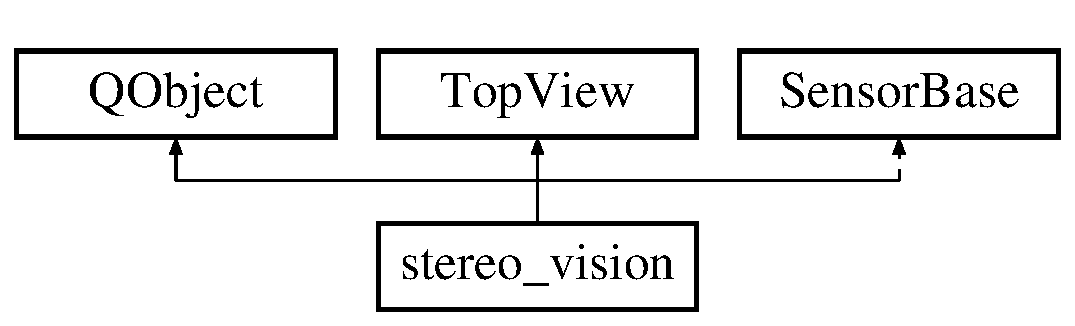
\includegraphics[height=2.000000cm]{classstereo__vision}
\end{center}
\end{figure}
\subsection*{Classes}
\begin{DoxyCompactItemize}
\item 
struct \hyperlink{structstereo__vision_1_1cam_param}{cam\+Param}
\begin{DoxyCompactList}\small\item\em The \hyperlink{structstereo__vision_1_1cam_param}{cam\+Param} struct for depth estimatiom. \end{DoxyCompactList}\item 
struct \hyperlink{structstereo__vision_1_1match_param_b_m}{match\+Param\+B\+M}
\item 
struct \hyperlink{structstereo__vision_1_1match_param_s_g_b_m}{match\+Param\+S\+G\+B\+M}
\item 
struct \hyperlink{structstereo__vision_1_1object_info}{object\+Info}
\item 
struct \hyperlink{structstereo__vision_1_1_stereo_data}{Stereo\+Data}
\begin{DoxyCompactList}\small\item\em The \hyperlink{structstereo__vision_1_1_stereo_data}{Stereo\+Data} struct. \end{DoxyCompactList}\end{DoxyCompactItemize}
\subsection*{Signals}
\begin{DoxyCompactItemize}
\item 
\hypertarget{classstereo__vision_afaa54843be42d382939a9b95df97a378}{}void {\bfseries update\+G\+U\+I} (cv\+::\+Mat $\ast$img\+\_\+\+L, cv\+::\+Mat $\ast$img\+\_\+\+R, cv\+::\+Mat $\ast$disp, cv\+::\+Mat $\ast$disp\+\_\+pseudo, cv\+::\+Mat $\ast$\hyperlink{class_top_view_a693454cfb21851b389634e28bdabe35a}{topview}, cv\+::\+Mat $\ast$img\+\_\+detected, int detected\+\_\+obj, int current\+\_\+frame\+\_\+count)\label{classstereo__vision_afaa54843be42d382939a9b95df97a378}

\item 
\hypertarget{classstereo__vision_aedbf17999d975ce6142527ffa9a32e24}{}void {\bfseries update\+Form} (int mode, std\+::vector$<$ int $>$ params)\label{classstereo__vision_aedbf17999d975ce6142527ffa9a32e24}

\item 
\hypertarget{classstereo__vision_a474c8ffdfea16eaac64e120bd6101b61}{}void {\bfseries video\+End} ()\label{classstereo__vision_a474c8ffdfea16eaac64e120bd6101b61}

\end{DoxyCompactItemize}
\subsection*{Public Member Functions}
\begin{DoxyCompactItemize}
\item 
bool \hyperlink{classstereo__vision_a5f10ebe6877fa06685259e7a14146857}{open} (int device\+\_\+index\+\_\+\+L, int device\+\_\+index\+\_\+\+R)
\begin{DoxyCompactList}\small\item\em open the cam. \end{DoxyCompactList}\item 
bool \hyperlink{classstereo__vision_a42d70e087c25b7b91d989b0f182f7efe}{is\+Opened} ()
\begin{DoxyCompactList}\small\item\em is\+Opened is to check if cam is opened or not \end{DoxyCompactList}\item 
\hypertarget{classstereo__vision_aa6323301b9c2a27f2bb01204dbca05f7}{}void \hyperlink{classstereo__vision_aa6323301b9c2a27f2bb01204dbca05f7}{close} ()\label{classstereo__vision_aa6323301b9c2a27f2bb01204dbca05f7}

\begin{DoxyCompactList}\small\item\em close cam. \end{DoxyCompactList}\item 
bool \hyperlink{classstereo__vision_a4d98bb5b8d89b9e085e21e3f687ab65c}{load\+Remap\+File} (int cam\+\_\+focal\+\_\+length, double base\+\_\+line)
\begin{DoxyCompactList}\small\item\em load\+Remap\+File for camera calibration. The folder of calibration files should be placed under project\textquotesingle{}s folder \end{DoxyCompactList}\item 
\hypertarget{classstereo__vision_af824225e48b0db6e7b2e97c36e947cd8}{}int {\bfseries data\+Exec} ()\label{classstereo__vision_af824225e48b0db6e7b2e97c36e947cd8}

\item 
\hypertarget{classstereo__vision_aac6e3f56cebb6c9db27e1f1ce96cf002}{}int {\bfseries obj\+Size} ()\label{classstereo__vision_aac6e3f56cebb6c9db27e1f1ce96cf002}

\item 
\hypertarget{classstereo__vision_a7b9aacf6f82eb8d38836bd1ad0a88873}{}int {\bfseries gui\+Update} ()\label{classstereo__vision_a7b9aacf6f82eb8d38836bd1ad0a88873}

\item 
\hypertarget{classstereo__vision_aa5823b967f14aa5fe353f0f7c983bbb7}{}bool {\bfseries fused\+Topview} ()\label{classstereo__vision_aa5823b967f14aa5fe353f0f7c983bbb7}

\item 
\hypertarget{classstereo__vision_a35f0b49b1839f2c05ee1c4bf381f7a2a}{}void {\bfseries Hough\+Line} ()\label{classstereo__vision_a35f0b49b1839f2c05ee1c4bf381f7a2a}

\item 
\hypertarget{classstereo__vision_a836c0c934401f062619d5d27ff763400}{}void {\bfseries get\+Mouse\+Cursor\+Info} (int y, int x, float \&disp, cv\+::\+Point3i \&pos3\+D)\label{classstereo__vision_a836c0c934401f062619d5d27ff763400}

\item 
\hypertarget{classstereo__vision_a77a08312396f01ff9e96b80db9636a83}{}void {\bfseries set\+Ground\+Filter} (bool fg\+\_\+enable)\label{classstereo__vision_a77a08312396f01ff9e96b80db9636a83}

\item 
\hypertarget{classstereo__vision_a57546410422adbce47c7e0db2f78261b}{}bool {\bfseries mode\+Changed} (int cur\+\_\+mode)\label{classstereo__vision_a57546410422adbce47c7e0db2f78261b}

\item 
\hypertarget{classstereo__vision_aa75b4dad19544a401f59aa527dd54697}{}void {\bfseries mode\+Change} (int cur\+\_\+mode, bool fg\+\_\+form\+\_\+smp\+\_\+update)\label{classstereo__vision_aa75b4dad19544a401f59aa527dd54697}

\item 
\hypertarget{classstereo__vision_a8ec3ea771d16660c9cd28ad6a451e2f8}{}void {\bfseries update\+Params\+Smp} ()\label{classstereo__vision_a8ec3ea771d16660c9cd28ad6a451e2f8}

\end{DoxyCompactItemize}
\subsection*{Public Attributes}
\begin{DoxyCompactItemize}
\item 
\hypertarget{classstereo__vision_aa158a1bbe77e1a54958572daf0a4ae52}{}int \hyperlink{classstereo__vision_aa158a1bbe77e1a54958572daf0a4ae52}{match\+\_\+mode}\label{classstereo__vision_aa158a1bbe77e1a54958572daf0a4ae52}

\begin{DoxyCompactList}\small\item\em stereo matching mode \end{DoxyCompactList}\item 
\hypertarget{classstereo__vision_aac7f078a0eeff8e85540641628911a46}{}std\+::vector$<$ int $>$ \hyperlink{classstereo__vision_aac7f078a0eeff8e85540641628911a46}{match\+\_\+param}\label{classstereo__vision_aac7f078a0eeff8e85540641628911a46}

\begin{DoxyCompactList}\small\item\em stereo matching params \end{DoxyCompactList}\item 
\hypertarget{classstereo__vision_a43efac70e2402b96dc47994dab82eef5}{}int {\bfseries time\+\_\+proc}\label{classstereo__vision_a43efac70e2402b96dc47994dab82eef5}

\item 
\hypertarget{classstereo__vision_a6d6580405e25800cc97bf10cd2be6ca7}{}cv\+::\+Mat {\bfseries img\+\_\+\+L}\label{classstereo__vision_a6d6580405e25800cc97bf10cd2be6ca7}

\item 
\hypertarget{classstereo__vision_abbbb2e0ea2ea99867db15bc9f4e7b735}{}cv\+::\+Mat {\bfseries img\+\_\+\+R}\label{classstereo__vision_abbbb2e0ea2ea99867db15bc9f4e7b735}

\item 
\hypertarget{classstereo__vision_a208e506dc490cce114a66060515a31f3}{}cv\+::\+Mat {\bfseries img\+\_\+r\+\_\+\+L}\label{classstereo__vision_a208e506dc490cce114a66060515a31f3}

\item 
\hypertarget{classstereo__vision_aba439f3d27de41b4c199158479a88c27}{}cv\+::\+Mat {\bfseries img\+\_\+r\+\_\+\+R}\label{classstereo__vision_aba439f3d27de41b4c199158479a88c27}

\item 
\hypertarget{classstereo__vision_ae600652d57c3918068298f50d5862b1f}{}cv\+::\+Mat {\bfseries img\+\_\+detected}\label{classstereo__vision_ae600652d57c3918068298f50d5862b1f}

\item 
\hypertarget{classstereo__vision_a4b4f5cedee0992e723f184d5ca0ef9cf}{}cv\+::\+Mat {\bfseries img\+\_\+detected\+\_\+display}\label{classstereo__vision_a4b4f5cedee0992e723f184d5ca0ef9cf}

\item 
\hypertarget{classstereo__vision_aa224d5b51573aab0080fe501ec13595f}{}int {\bfseries input\+\_\+mode}\label{classstereo__vision_aa224d5b51573aab0080fe501ec13595f}

\item 
\hypertarget{classstereo__vision_a43d90438c1816a2d8ea75bf70fa66ad9}{}bool \hyperlink{classstereo__vision_a43d90438c1816a2d8ea75bf70fa66ad9}{fg\+\_\+calib}\label{classstereo__vision_a43d90438c1816a2d8ea75bf70fa66ad9}

\begin{DoxyCompactList}\small\item\em check whether the calibration button is checked \end{DoxyCompactList}\item 
\hypertarget{classstereo__vision_aa4cd54587f4089a1780ee3b3e622720f}{}bool \hyperlink{classstereo__vision_aa4cd54587f4089a1780ee3b3e622720f}{fg\+\_\+stereo\+Match}\label{classstereo__vision_aa4cd54587f4089a1780ee3b3e622720f}

\begin{DoxyCompactList}\small\item\em check whether do the correspondence matching \end{DoxyCompactList}\item 
\hypertarget{classstereo__vision_a9046c0d1af87b98a5848070199a980ba}{}bool \hyperlink{classstereo__vision_a9046c0d1af87b98a5848070199a980ba}{fg\+\_\+pseudo}\label{classstereo__vision_a9046c0d1af87b98a5848070199a980ba}

\begin{DoxyCompactList}\small\item\em chekc wether pesudo the disparity image \end{DoxyCompactList}\item 
\hypertarget{classstereo__vision_a46c04908475380f5901a0a7a08f5643c}{}bool \hyperlink{classstereo__vision_a46c04908475380f5901a0a7a08f5643c}{fg\+\_\+topview}\label{classstereo__vision_a46c04908475380f5901a0a7a08f5643c}

\begin{DoxyCompactList}\small\item\em check wether project to topview \end{DoxyCompactList}\item 
\hypertarget{classstereo__vision_ab1be52b3eb3c5629d81655fbc5dab14d}{}bool \hyperlink{classstereo__vision_ab1be52b3eb3c5629d81655fbc5dab14d}{fg\+\_\+reproject}\label{classstereo__vision_ab1be52b3eb3c5629d81655fbc5dab14d}

\begin{DoxyCompactList}\small\item\em check wether re-\/project detected objects to image \end{DoxyCompactList}\item 
\hypertarget{classstereo__vision_aa887dac1c609d96131aba8c2c386b8b4}{}bool \hyperlink{classstereo__vision_aa887dac1c609d96131aba8c2c386b8b4}{fg\+\_\+tracking}\label{classstereo__vision_aa887dac1c609d96131aba8c2c386b8b4}

\begin{DoxyCompactList}\small\item\em it\textquotesingle{}s true when object tracking is activated \end{DoxyCompactList}\item 
\hypertarget{classstereo__vision_af3c1db66e4aee9b6cb699ad83208017e}{}bool \hyperlink{classstereo__vision_af3c1db66e4aee9b6cb699ad83208017e}{fg\+\_\+topview\+\_\+plot\+\_\+points}\label{classstereo__vision_af3c1db66e4aee9b6cb699ad83208017e}

\begin{DoxyCompactList}\small\item\em check wethere to plot each points on the topview \end{DoxyCompactList}\item 
\hypertarget{classstereo__vision_a208843ce79040143215a89c09441fac6}{}cv\+::\+Mat {\bfseries disp\+\_\+raw}\label{classstereo__vision_a208843ce79040143215a89c09441fac6}

\item 
\hypertarget{classstereo__vision_aff10e9a2deaad5be0fe0f5282a40d89d}{}cv\+::\+Mat {\bfseries disp}\label{classstereo__vision_aff10e9a2deaad5be0fe0f5282a40d89d}

\item 
\hypertarget{classstereo__vision_a9bc79f927c68742c44ed169dd0ac7c0c}{}cv\+::\+Mat {\bfseries disp\+\_\+pseudo}\label{classstereo__vision_a9bc79f927c68742c44ed169dd0ac7c0c}

\item 
\hypertarget{classstereo__vision_a116de235ec3af6a1fbf32e53553e7fff}{}\hyperlink{structstereo__vision_1_1cam_param}{cam\+Param} $\ast$ {\bfseries cam\+\_\+param}\label{classstereo__vision_a116de235ec3af6a1fbf32e53553e7fff}

\item 
\hypertarget{classstereo__vision_abe67917e4552e10eec02cf1df85548bd}{}\hyperlink{structstereo__vision_1_1_stereo_data}{Stereo\+Data} $\ast$$\ast$ {\bfseries data}\label{classstereo__vision_abe67917e4552e10eec02cf1df85548bd}

\item 
\hypertarget{classstereo__vision_aa62f831945967b161fdf8c2c08edf98e}{}\hyperlink{structstereo__vision_1_1match_param_s_g_b_m}{match\+Param\+S\+G\+B\+M} $\ast$ {\bfseries param\+\_\+sgbm}\label{classstereo__vision_aa62f831945967b161fdf8c2c08edf98e}

\item 
\hypertarget{classstereo__vision_a4d6e2801a81407b8cbcb9e82a8217d39}{}\hyperlink{structstereo__vision_1_1match_param_b_m}{match\+Param\+B\+M} $\ast$ {\bfseries param\+\_\+bm}\label{classstereo__vision_a4d6e2801a81407b8cbcb9e82a8217d39}

\item 
\hypertarget{classstereo__vision_a22a8e8ee420a6a7e3d602cc363e83f25}{}int {\bfseries thick\+\_\+obj\+\_\+rect}\label{classstereo__vision_a22a8e8ee420a6a7e3d602cc363e83f25}

\item 
\hypertarget{classstereo__vision_a6ef6db60b0aa3e917192bb1ec2e5f464}{}int {\bfseries radius\+\_\+obj\+\_\+point}\label{classstereo__vision_a6ef6db60b0aa3e917192bb1ec2e5f464}

\item 
\hypertarget{classstereo__vision_a119f4b3f00d991d11608ec8a75c7434c}{}\hyperlink{structstereo__vision_1_1object_info}{object\+Info} $\ast$ {\bfseries objects\+\_\+display}\label{classstereo__vision_a119f4b3f00d991d11608ec8a75c7434c}

\end{DoxyCompactItemize}
\subsection*{Private Slots}
\begin{DoxyCompactItemize}
\item 
\hypertarget{classstereo__vision_aa0319c83d83972c5e2946471248e75c7}{}void {\bfseries change\+\_\+bm\+\_\+pre\+\_\+filter\+\_\+size} (int value)\label{classstereo__vision_aa0319c83d83972c5e2946471248e75c7}

\item 
\hypertarget{classstereo__vision_a88c796355054746b0c710f854a131a76}{}void {\bfseries change\+\_\+bm\+\_\+pre\+\_\+filter\+\_\+cap} (int value)\label{classstereo__vision_a88c796355054746b0c710f854a131a76}

\item 
\hypertarget{classstereo__vision_a8121a10f1e88f8927e95216b4cac24f5}{}void {\bfseries change\+\_\+bm\+\_\+sad\+\_\+window\+\_\+size} (int value)\label{classstereo__vision_a8121a10f1e88f8927e95216b4cac24f5}

\item 
\hypertarget{classstereo__vision_a67bc5743196841e228c689dbb24836fc}{}void {\bfseries change\+\_\+bm\+\_\+min\+\_\+disp} (int value)\label{classstereo__vision_a67bc5743196841e228c689dbb24836fc}

\item 
\hypertarget{classstereo__vision_a383e31f5004624e7b733614d795560a8}{}void {\bfseries change\+\_\+bm\+\_\+num\+\_\+of\+\_\+disp} (int value)\label{classstereo__vision_a383e31f5004624e7b733614d795560a8}

\item 
\hypertarget{classstereo__vision_aa46cd94d569e6b081232df19b218e48f}{}void {\bfseries change\+\_\+bm\+\_\+texture\+\_\+thresh} (int value)\label{classstereo__vision_aa46cd94d569e6b081232df19b218e48f}

\item 
\hypertarget{classstereo__vision_ab8d73fb75b7b288c893a5d67fa88723c}{}void {\bfseries change\+\_\+bm\+\_\+uniqueness\+\_\+ratio} (int value)\label{classstereo__vision_ab8d73fb75b7b288c893a5d67fa88723c}

\item 
\hypertarget{classstereo__vision_a26a1e11b0500bb2aff38c8fe38d0bbcb}{}void {\bfseries change\+\_\+bm\+\_\+speckle\+\_\+window\+\_\+size} (int value)\label{classstereo__vision_a26a1e11b0500bb2aff38c8fe38d0bbcb}

\item 
\hypertarget{classstereo__vision_ad6fc54a9e01b8890f55a9f74a2fca828}{}void {\bfseries change\+\_\+bm\+\_\+speckle\+\_\+range} (int value)\label{classstereo__vision_ad6fc54a9e01b8890f55a9f74a2fca828}

\item 
\hypertarget{classstereo__vision_a09335560bab92800a363ff9331eff0b2}{}void {\bfseries change\+\_\+sgbm\+\_\+pre\+\_\+filter\+\_\+cap} (int value)\label{classstereo__vision_a09335560bab92800a363ff9331eff0b2}

\item 
\hypertarget{classstereo__vision_ab46602e71890356be13aaaad67839161}{}void {\bfseries change\+\_\+sgbm\+\_\+sad\+\_\+window\+\_\+size} (int value)\label{classstereo__vision_ab46602e71890356be13aaaad67839161}

\item 
\hypertarget{classstereo__vision_a0e045f3e764dc05a7996eafcaf8aebc6}{}void {\bfseries change\+\_\+sgbm\+\_\+min\+\_\+disp} (int value)\label{classstereo__vision_a0e045f3e764dc05a7996eafcaf8aebc6}

\item 
\hypertarget{classstereo__vision_aefbefa16ef9ddeb42ae10133993df641}{}void {\bfseries change\+\_\+sgbm\+\_\+num\+\_\+of\+\_\+disp} (int value)\label{classstereo__vision_aefbefa16ef9ddeb42ae10133993df641}

\item 
\hypertarget{classstereo__vision_adef75037844513259388033ab8e19e8d}{}void {\bfseries change\+\_\+sgbm\+\_\+uniqueness\+\_\+ratio} (int value)\label{classstereo__vision_adef75037844513259388033ab8e19e8d}

\item 
\hypertarget{classstereo__vision_a504e03ec97c53c7d90a10541351c8d52}{}void {\bfseries change\+\_\+sgbm\+\_\+speckle\+\_\+window\+\_\+size} (int value)\label{classstereo__vision_a504e03ec97c53c7d90a10541351c8d52}

\item 
\hypertarget{classstereo__vision_aa8fc24479b5dd2252de370f9bfd35823}{}void {\bfseries change\+\_\+sgbm\+\_\+speckle\+\_\+range} (int value)\label{classstereo__vision_aa8fc24479b5dd2252de370f9bfd35823}

\end{DoxyCompactItemize}
\subsection*{Private Member Functions}
\begin{DoxyCompactItemize}
\item 
\hypertarget{classstereo__vision_af59672af6aac7231b711998a881a6207}{}void {\bfseries create\+L\+U\+T} ()\label{classstereo__vision_af59672af6aac7231b711998a881a6207}

\item 
\hypertarget{classstereo__vision_a9ba04ac316db4e0eafc80916309374d4}{}int {\bfseries corr\+Grid\+Row} (int \hyperlink{class_top_view_a1f2b530e7979db621630dbbf9f5def15}{k})\label{classstereo__vision_a9ba04ac316db4e0eafc80916309374d4}

\item 
\hypertarget{classstereo__vision_a1921e6d848a96c9989a0a86b4ef9fd82}{}int {\bfseries corr\+Grid\+Col} (int \hyperlink{class_top_view_a1f2b530e7979db621630dbbf9f5def15}{k})\label{classstereo__vision_a1921e6d848a96c9989a0a86b4ef9fd82}

\item 
\hypertarget{classstereo__vision_ad8a2dff52e5b5dc21eab2203dbb17d3a}{}void {\bfseries reset\+Open} (int device\+\_\+index\+\_\+\+L, int device\+\_\+index\+\_\+\+R)\label{classstereo__vision_ad8a2dff52e5b5dc21eab2203dbb17d3a}

\item 
\hypertarget{classstereo__vision_a107d39b128afb19544c842bb960dfcc1}{}bool {\bfseries cam\+Capture} ()\label{classstereo__vision_a107d39b128afb19544c842bb960dfcc1}

\item 
\hypertarget{classstereo__vision_a85ad1d14a5813f89e5b2ba48a4951cc1}{}bool {\bfseries data\+In} ()\label{classstereo__vision_a85ad1d14a5813f89e5b2ba48a4951cc1}

\item 
\hypertarget{classstereo__vision_a438714bfc63e25fa55509422d10909a4}{}bool {\bfseries rectify\+Image} ()\label{classstereo__vision_a438714bfc63e25fa55509422d10909a4}

\item 
\hypertarget{classstereo__vision_aac941ae2043d7e1034d002033e6cf3d0}{}void {\bfseries depth\+Calculation} ()\label{classstereo__vision_aac941ae2043d7e1034d002033e6cf3d0}

\item 
\hypertarget{classstereo__vision_aa8e6fc4e5d1a8447baa53a64ba4d2a9f}{}bool {\bfseries v\+Disp\+Calculation} ()\label{classstereo__vision_aa8e6fc4e5d1a8447baa53a64ba4d2a9f}

\item 
\hypertarget{classstereo__vision_a45dc1b4c26fa70b641ad31f4b307f0c8}{}float {\bfseries point2\+Line} (cv\+::\+Point pt, cv\+::\+Point line\+\_\+1, cv\+::\+Point line\+\_\+2)\label{classstereo__vision_a45dc1b4c26fa70b641ad31f4b307f0c8}

\item 
\hypertarget{classstereo__vision_a74c36c45aa91e35150ceb51c3ddf0c03}{}void {\bfseries stereo\+Match} ()\label{classstereo__vision_a74c36c45aa91e35150ceb51c3ddf0c03}

\item 
\hypertarget{classstereo__vision_aa809afbb9b4bcf9430a12d3fe2bf0a83}{}void {\bfseries update\+Form\+Params} ()\label{classstereo__vision_aa809afbb9b4bcf9430a12d3fe2bf0a83}

\item 
\hypertarget{classstereo__vision_acb993e7cbfb1a1745fcc3cc4b7ad4aaa}{}void {\bfseries update\+Data\+For\+Display} ()\label{classstereo__vision_acb993e7cbfb1a1745fcc3cc4b7ad4aaa}

\item 
\hypertarget{classstereo__vision_a6928cbfd7d4ee3834d3ef9b4f2fe4588}{}void {\bfseries reset\+Blob} ()\label{classstereo__vision_a6928cbfd7d4ee3834d3ef9b4f2fe4588}

\item 
\hypertarget{classstereo__vision_ac9520d8ca3fe11aba04a5d11a65ee0df}{}void {\bfseries blob} (int thresh\+\_\+pts\+\_\+num)\label{classstereo__vision_ac9520d8ca3fe11aba04a5d11a65ee0df}

\item 
\hypertarget{classstereo__vision_ab8b62349e5049fe2d61e3de5a2d5477c}{}void {\bfseries reset\+Matched\+Info} (\hyperlink{structstereo__vision_1_1object_info}{object\+Info} \&src)\label{classstereo__vision_ab8b62349e5049fe2d61e3de5a2d5477c}

\item 
\hypertarget{classstereo__vision_a541abf632d62e399866cd7d265673063}{}void {\bfseries connect\+Matched\+Info} (\hyperlink{structstereo__vision_1_1object_info}{object\+Info} \&src, \hyperlink{structstereo__vision_1_1object_info}{object\+Info} \&dst)\label{classstereo__vision_a541abf632d62e399866cd7d265673063}

\item 
\hypertarget{classstereo__vision_a99a62cb0c6c16f46d420b5f4d0379a48}{}void {\bfseries match\+Param\+Initialize} (int cur\+\_\+mode)\label{classstereo__vision_a99a62cb0c6c16f46d420b5f4d0379a48}

\item 
\hypertarget{classstereo__vision_aa3fd13ec1a7eec08eb964e5339d653f6}{}void {\bfseries point\+Project\+Top\+View} ()\label{classstereo__vision_aa3fd13ec1a7eec08eb964e5339d653f6}

\item 
\hypertarget{classstereo__vision_a265f15ae20bfad32d0b3091c29d54021}{}void {\bfseries point\+Project\+Image} ()\label{classstereo__vision_a265f15ae20bfad32d0b3091c29d54021}

\end{DoxyCompactItemize}
\subsection*{Private Attributes}
\begin{DoxyCompactItemize}
\item 
\hypertarget{classstereo__vision_ac22d7d1d46c44012d977fc6a7a4b294b}{}int $\ast$ {\bfseries L\+U\+T\+\_\+grid\+\_\+row}\label{classstereo__vision_ac22d7d1d46c44012d977fc6a7a4b294b}

\item 
\hypertarget{classstereo__vision_a533641d0d10bb6958b20c0779e44bac3}{}int $\ast$ {\bfseries L\+U\+T\+\_\+grid\+\_\+col}\label{classstereo__vision_a533641d0d10bb6958b20c0779e44bac3}

\item 
\hypertarget{classstereo__vision_a436f56ee5dafff4cd4a1c0d1d9295389}{}int $\ast$ {\bfseries L\+U\+T\+\_\+depth}\label{classstereo__vision_a436f56ee5dafff4cd4a1c0d1d9295389}

\item 
\hypertarget{classstereo__vision_ae49394206441102638ca0b3cd573a7ff}{}int $\ast$ {\bfseries L\+U\+T\+\_\+img\+\_\+col}\label{classstereo__vision_ae49394206441102638ca0b3cd573a7ff}

\item 
\hypertarget{classstereo__vision_a44fc71a48835c0e82473405226959758}{}Q\+Time {\bfseries t\+\_\+p}\label{classstereo__vision_a44fc71a48835c0e82473405226959758}

\item 
\hypertarget{classstereo__vision_a0327c8570c58bb5e263284a6b07826b7}{}bool {\bfseries fg\+\_\+cam\+\_\+\+L}\label{classstereo__vision_a0327c8570c58bb5e263284a6b07826b7}

\item 
\hypertarget{classstereo__vision_a849dd6a5a5c90a89e60237709f681db0}{}bool {\bfseries fg\+\_\+cam\+\_\+\+R}\label{classstereo__vision_a849dd6a5a5c90a89e60237709f681db0}

\item 
\hypertarget{classstereo__vision_acc86e620bc551a4c464204185b9ba688}{}bool {\bfseries fg\+\_\+cam\+\_\+opened}\label{classstereo__vision_acc86e620bc551a4c464204185b9ba688}

\item 
\hypertarget{classstereo__vision_abe770e5693436ece0f050c46639aced2}{}bool {\bfseries fg\+\_\+calib\+\_\+loaded}\label{classstereo__vision_abe770e5693436ece0f050c46639aced2}

\item 
\hypertarget{classstereo__vision_ae0c3398306a273523a736b912fe17669}{}Q\+Time {\bfseries t}\label{classstereo__vision_ae0c3398306a273523a736b912fe17669}

\item 
\hypertarget{classstereo__vision_a5ad6c9bb31ff5e99c6dee350c8b294d0}{}int {\bfseries time\+\_\+gap}\label{classstereo__vision_a5ad6c9bb31ff5e99c6dee350c8b294d0}

\item 
\hypertarget{classstereo__vision_aa6a17817d8ec47b9b62e8c5122254d1b}{}int {\bfseries device\+\_\+index\+\_\+\+L}\label{classstereo__vision_aa6a17817d8ec47b9b62e8c5122254d1b}

\item 
\hypertarget{classstereo__vision_a5ae8c08b9a449d612e5d7ce9a10005e0}{}int {\bfseries device\+\_\+index\+\_\+\+R}\label{classstereo__vision_a5ae8c08b9a449d612e5d7ce9a10005e0}

\item 
\hypertarget{classstereo__vision_a22e41793b6720792bd992d31ff1bf4d0}{}cv\+::\+Video\+Capture {\bfseries cam\+\_\+\+L}\label{classstereo__vision_a22e41793b6720792bd992d31ff1bf4d0}

\item 
\hypertarget{classstereo__vision_a567e69673b327e4c778069cc289e4ed8}{}cv\+::\+Video\+Capture {\bfseries cam\+\_\+\+R}\label{classstereo__vision_a567e69673b327e4c778069cc289e4ed8}

\item 
\hypertarget{classstereo__vision_ad4560f29f1d3b52e1cb284123e9afb7a}{}cv\+::\+Mat {\bfseries cap\+\_\+\+L}\label{classstereo__vision_ad4560f29f1d3b52e1cb284123e9afb7a}

\item 
\hypertarget{classstereo__vision_ab9a196d52aac1f1b7840b25fe5c59f6b}{}cv\+::\+Mat {\bfseries cap\+\_\+\+R}\label{classstereo__vision_ab9a196d52aac1f1b7840b25fe5c59f6b}

\item 
\hypertarget{classstereo__vision_acebe9a3bf44da123652d784446142288}{}Q\+Dir {\bfseries remap\+\_\+path}\label{classstereo__vision_acebe9a3bf44da123652d784446142288}

\item 
\hypertarget{classstereo__vision_a4568f181500db97d44dfbb9c1275c23b}{}Q\+String {\bfseries remap\+\_\+folder}\label{classstereo__vision_a4568f181500db97d44dfbb9c1275c23b}

\item 
\hypertarget{classstereo__vision_a0c645f23171054cb8b97110d5086d02b}{}Q\+String {\bfseries remap\+\_\+file}\label{classstereo__vision_a0c645f23171054cb8b97110d5086d02b}

\item 
\hypertarget{classstereo__vision_a0d5323c5ba071c0e3a6fb8e8cb70c4f8}{}cv\+::\+Mat {\bfseries rmap\+Lx}\label{classstereo__vision_a0d5323c5ba071c0e3a6fb8e8cb70c4f8}

\item 
\hypertarget{classstereo__vision_ab148fbd46aad800d51f38e0ea6c88b0c}{}cv\+::\+Mat {\bfseries rmap\+Ly}\label{classstereo__vision_ab148fbd46aad800d51f38e0ea6c88b0c}

\item 
\hypertarget{classstereo__vision_a9d544e26683b6df416d13c15cda4e86e}{}cv\+::\+Mat {\bfseries rmap\+Rx}\label{classstereo__vision_a9d544e26683b6df416d13c15cda4e86e}

\item 
\hypertarget{classstereo__vision_a815c5a01f2352328642ece249e581c70}{}cv\+::\+Mat {\bfseries rmap\+Ry}\label{classstereo__vision_a815c5a01f2352328642ece249e581c70}

\item 
\hypertarget{classstereo__vision_acbb4008c31a3fa4e00598b4c34433c95}{}cv\+::\+Rect {\bfseries calib\+R\+O\+I} \mbox{[}2\mbox{]}\label{classstereo__vision_acbb4008c31a3fa4e00598b4c34433c95}

\item 
\hypertarget{classstereo__vision_ab64d35e2fd18e3db6a198a556a264d89}{}cv\+::\+Ptr$<$ cv\+::\+Stereo\+S\+G\+B\+M $>$ {\bfseries sgbm}\label{classstereo__vision_ab64d35e2fd18e3db6a198a556a264d89}

\item 
\hypertarget{classstereo__vision_af6ab96352f2db952e9d453f6206eecba}{}cv\+::\+Ptr$<$ cv\+::\+Stereo\+B\+M $>$ {\bfseries bm}\label{classstereo__vision_af6ab96352f2db952e9d453f6206eecba}

\item 
\hypertarget{classstereo__vision_ad01965e56dd61dffb297d766ec45a00c}{}int {\bfseries cn}\label{classstereo__vision_ad01965e56dd61dffb297d766ec45a00c}

\item 
\hypertarget{classstereo__vision_ad50feb2fb1ac107ec61cba14f1f211be}{}cv\+::\+Mat {\bfseries img\+\_\+match\+\_\+\+L}\label{classstereo__vision_ad50feb2fb1ac107ec61cba14f1f211be}

\item 
\hypertarget{classstereo__vision_aa68a9b9eb2a44afd446d77c04e32400d}{}cv\+::\+Mat {\bfseries img\+\_\+match\+\_\+\+R}\label{classstereo__vision_aa68a9b9eb2a44afd446d77c04e32400d}

\item 
\hypertarget{classstereo__vision_a783032355f08f98513645fdbf37bc76b}{}int {\bfseries obj\+\_\+nums}\label{classstereo__vision_a783032355f08f98513645fdbf37bc76b}

\item 
\hypertarget{classstereo__vision_ad13625d9a57b2ab1201859a15ae7a1d4}{}\hyperlink{structstereo__vision_1_1object_info}{object\+Info} $\ast$ {\bfseries objects}\label{classstereo__vision_ad13625d9a57b2ab1201859a15ae7a1d4}

\item 
\hypertarget{classstereo__vision_a88866738f710fa7f1c160113fd97f7ea}{}int {\bfseries detected\+\_\+obj}\label{classstereo__vision_a88866738f710fa7f1c160113fd97f7ea}

\item 
\hypertarget{classstereo__vision_a6f4b09547d0a4b0d46c229378b1012d5}{}\hyperlink{structstereo__vision_1_1object_info}{object\+Info} {\bfseries obj\+\_\+temp}\label{classstereo__vision_a6f4b09547d0a4b0d46c229378b1012d5}

\item 
\hypertarget{classstereo__vision_a124bffa45f264820eee7825de3f4eab4}{}int {\bfseries thresh\+\_\+ground\+\_\+cand}\label{classstereo__vision_a124bffa45f264820eee7825de3f4eab4}

\item 
\hypertarget{classstereo__vision_ab7d89707e6e5f29e42e93af3afe38247}{}float {\bfseries ground\+\_\+mean\+\_\+guess}\label{classstereo__vision_ab7d89707e6e5f29e42e93af3afe38247}

\item 
\hypertarget{classstereo__vision_a8c521a7a88202b9415f4f618d7e742c2}{}bool {\bfseries fg\+\_\+ground\+\_\+filter}\label{classstereo__vision_a8c521a7a88202b9415f4f618d7e742c2}

\item 
\hypertarget{classstereo__vision_af54c2344e37afb042efb20ca0e1fddb1}{}bool {\bfseries fg\+\_\+v\+Disp}\label{classstereo__vision_af54c2344e37afb042efb20ca0e1fddb1}

\item 
\hypertarget{classstereo__vision_a9f04ffbae5362d509b1e3d4b1ab58600}{}double {\bfseries angle\+\_\+min}\label{classstereo__vision_a9f04ffbae5362d509b1e3d4b1ab58600}

\item 
\hypertarget{classstereo__vision_a4d6622be3a7ccd00379d6a9af3891eec}{}double {\bfseries angle\+\_\+max}\label{classstereo__vision_a4d6622be3a7ccd00379d6a9af3891eec}

\item 
\hypertarget{classstereo__vision_a53da08e1e23e839b2b6d1c2ab0ed6018}{}float {\bfseries thresh\+\_\+rho\+\_\+min}\label{classstereo__vision_a53da08e1e23e839b2b6d1c2ab0ed6018}

\item 
\hypertarget{classstereo__vision_af14a8db25f5d53e9e4e2b3ffaceec2fd}{}float {\bfseries thresh\+\_\+ground\+\_\+y\+\_\+max}\label{classstereo__vision_af14a8db25f5d53e9e4e2b3ffaceec2fd}

\item 
\hypertarget{classstereo__vision_a378c5c38f91af6f92b338e563b15631b}{}float {\bfseries thresh\+\_\+dist}\label{classstereo__vision_a378c5c38f91af6f92b338e563b15631b}

\item 
\hypertarget{classstereo__vision_a6f58586dded0f2e9658a741400043ba3}{}float {\bfseries weight\+\_\+now}\label{classstereo__vision_a6f58586dded0f2e9658a741400043ba3}

\item 
\hypertarget{classstereo__vision_a3911a0a28a821f478afb76f2b22c0183}{}float {\bfseries weight\+\_\+prev}\label{classstereo__vision_a3911a0a28a821f478afb76f2b22c0183}

\item 
\hypertarget{classstereo__vision_ae8e557c8dd6934d110c020fde6559b57}{}std\+::vector$<$ cv\+::\+Vec2f $>$ {\bfseries lines}\label{classstereo__vision_ae8e557c8dd6934d110c020fde6559b57}

\item 
\hypertarget{classstereo__vision_a28ce31b7e25d89b2722c1b3a59638a5b}{}std\+::vector$<$ int $>$ {\bfseries lines\+\_\+fitted\+\_\+pt}\label{classstereo__vision_a28ce31b7e25d89b2722c1b3a59638a5b}

\item 
\hypertarget{classstereo__vision_a4c8c4d4ded884967455a4191da99b3ab}{}cv\+::\+Vec2f {\bfseries fitted\+\_\+line}\label{classstereo__vision_a4c8c4d4ded884967455a4191da99b3ab}

\item 
\hypertarget{classstereo__vision_aca6fe3ca55cc9d96d1ce0d865528aca8}{}cv\+::\+Mat {\bfseries v\+\_\+disp}\label{classstereo__vision_aca6fe3ca55cc9d96d1ce0d865528aca8}

\item 
\hypertarget{classstereo__vision_aeefaec8a3326aa2dfc460032ee5a1aa7}{}cv\+::\+Mat {\bfseries v\+\_\+disp\+\_\+norm}\label{classstereo__vision_aeefaec8a3326aa2dfc460032ee5a1aa7}

\item 
\hypertarget{classstereo__vision_a2cb73a0711a7d2a456b5b9183df49b05}{}cv\+::\+Mat {\bfseries v\+\_\+disp\+\_\+display}\label{classstereo__vision_a2cb73a0711a7d2a456b5b9183df49b05}

\item 
\hypertarget{classstereo__vision_a2b9620ac49c42868cae704f319cf9eea}{}cv\+::\+Mat {\bfseries v\+\_\+disp\+\_\+bi}\label{classstereo__vision_a2b9620ac49c42868cae704f319cf9eea}

\end{DoxyCompactItemize}
\subsection*{Additional Inherited Members}


\subsection{Member Function Documentation}
\hypertarget{classstereo__vision_a42d70e087c25b7b91d989b0f182f7efe}{}\index{stereo\+\_\+vision@{stereo\+\_\+vision}!is\+Opened@{is\+Opened}}
\index{is\+Opened@{is\+Opened}!stereo\+\_\+vision@{stereo\+\_\+vision}}
\subsubsection[{is\+Opened}]{\setlength{\rightskip}{0pt plus 5cm}bool stereo\+\_\+vision\+::is\+Opened (
\begin{DoxyParamCaption}
{}
\end{DoxyParamCaption}
)\hspace{0.3cm}{\ttfamily [inline]}}\label{classstereo__vision_a42d70e087c25b7b91d989b0f182f7efe}


is\+Opened is to check if cam is opened or not 

\begin{DoxyReturn}{Returns}

\end{DoxyReturn}
\hypertarget{classstereo__vision_a4d98bb5b8d89b9e085e21e3f687ab65c}{}\index{stereo\+\_\+vision@{stereo\+\_\+vision}!load\+Remap\+File@{load\+Remap\+File}}
\index{load\+Remap\+File@{load\+Remap\+File}!stereo\+\_\+vision@{stereo\+\_\+vision}}
\subsubsection[{load\+Remap\+File}]{\setlength{\rightskip}{0pt plus 5cm}bool stereo\+\_\+vision\+::load\+Remap\+File (
\begin{DoxyParamCaption}
\item[{int}]{cam\+\_\+focal\+\_\+length, }
\item[{double}]{base\+\_\+line}
\end{DoxyParamCaption}
)}\label{classstereo__vision_a4d98bb5b8d89b9e085e21e3f687ab65c}


load\+Remap\+File for camera calibration. The folder of calibration files should be placed under project\textquotesingle{}s folder 


\begin{DoxyParams}{Parameters}
{\em cam\+\_\+focal\+\_\+length} & \\
\hline
{\em base\+\_\+line} & \\
\hline
\end{DoxyParams}
\begin{DoxyReturn}{Returns}

\end{DoxyReturn}
\hypertarget{classstereo__vision_a5f10ebe6877fa06685259e7a14146857}{}\index{stereo\+\_\+vision@{stereo\+\_\+vision}!open@{open}}
\index{open@{open}!stereo\+\_\+vision@{stereo\+\_\+vision}}
\subsubsection[{open}]{\setlength{\rightskip}{0pt plus 5cm}bool stereo\+\_\+vision\+::open (
\begin{DoxyParamCaption}
\item[{int}]{device\+\_\+index\+\_\+\+L, }
\item[{int}]{device\+\_\+index\+\_\+\+R}
\end{DoxyParamCaption}
)}\label{classstereo__vision_a5f10ebe6877fa06685259e7a14146857}


open the cam. 


\begin{DoxyParams}{Parameters}
{\em device\+\_\+index\+\_\+\+L} & \\
\hline
{\em device\+\_\+index\+\_\+\+R} & \\
\hline
\end{DoxyParams}
\begin{DoxyReturn}{Returns}

\end{DoxyReturn}


The documentation for this class was generated from the following files\+:\begin{DoxyCompactItemize}
\item 
D\+:/\+Qt\+Program/\+Qt5/\+Fusion/stereo\+\_\+vision.\+h\item 
D\+:/\+Qt\+Program/\+Qt5/\+Fusion/stereo\+\_\+vision.\+cpp\end{DoxyCompactItemize}

\hypertarget{structstereo__vision_1_1_stereo_data}{}\section{stereo\+\_\+vision\+:\+:Stereo\+Data Struct Reference}
\label{structstereo__vision_1_1_stereo_data}\index{stereo\+\_\+vision\+::\+Stereo\+Data@{stereo\+\_\+vision\+::\+Stereo\+Data}}


The \hyperlink{structstereo__vision_1_1_stereo_data}{Stereo\+Data} struct.  




{\ttfamily \#include $<$stereo\+\_\+vision.\+h$>$}

\subsection*{Public Attributes}
\begin{DoxyCompactItemize}
\item 
\hypertarget{structstereo__vision_1_1_stereo_data_a64a63da05bda0b911b580017907d3cd4}{}float {\bfseries disp}\label{structstereo__vision_1_1_stereo_data_a64a63da05bda0b911b580017907d3cd4}

\item 
\hypertarget{structstereo__vision_1_1_stereo_data_a020c1abf7b53ad7553f05e9a1cbceafc}{}int {\bfseries X}\label{structstereo__vision_1_1_stereo_data_a020c1abf7b53ad7553f05e9a1cbceafc}

\item 
\hypertarget{structstereo__vision_1_1_stereo_data_ae018bd15ad3a913268b3c0be446dcec2}{}int {\bfseries Y}\label{structstereo__vision_1_1_stereo_data_ae018bd15ad3a913268b3c0be446dcec2}

\item 
\hypertarget{structstereo__vision_1_1_stereo_data_a3223806159a7fc90ee6d523c89346bcd}{}int {\bfseries Z}\label{structstereo__vision_1_1_stereo_data_a3223806159a7fc90ee6d523c89346bcd}

\item 
\hypertarget{structstereo__vision_1_1_stereo_data_ac1742b7a708e1cc995fc26e046551272}{}bool \hyperlink{structstereo__vision_1_1_stereo_data_ac1742b7a708e1cc995fc26e046551272}{ground\+\_\+cand}\label{structstereo__vision_1_1_stereo_data_ac1742b7a708e1cc995fc26e046551272}

\begin{DoxyCompactList}\small\item\em recognized as ground by v-\/disparity algorithm \end{DoxyCompactList}\item 
\hypertarget{structstereo__vision_1_1_stereo_data_ad224fb4fb920f605c9ef909b799b8785}{}std\+::pair$<$ int, int $>$ \hyperlink{structstereo__vision_1_1_stereo_data_ad224fb4fb920f605c9ef909b799b8785}{grid\+\_\+id}\label{structstereo__vision_1_1_stereo_data_ad224fb4fb920f605c9ef909b799b8785}

\begin{DoxyCompactList}\small\item\em located cell in topview \end{DoxyCompactList}\end{DoxyCompactItemize}


\subsection{Detailed Description}
The \hyperlink{structstereo__vision_1_1_stereo_data}{Stereo\+Data} struct. 

The documentation for this struct was generated from the following file\+:\begin{DoxyCompactItemize}
\item 
D\+:/\+Qt\+Program/\+Qt5/\+Fusion/stereo\+\_\+vision.\+h\end{DoxyCompactItemize}

\hypertarget{class_ui_1_1stereo_match_param_form}{}\section{Ui\+:\+:stereo\+Match\+Param\+Form Class Reference}
\label{class_ui_1_1stereo_match_param_form}\index{Ui\+::stereo\+Match\+Param\+Form@{Ui\+::stereo\+Match\+Param\+Form}}
Inheritance diagram for Ui\+:\+:stereo\+Match\+Param\+Form\+:\begin{figure}[H]
\begin{center}
\leavevmode
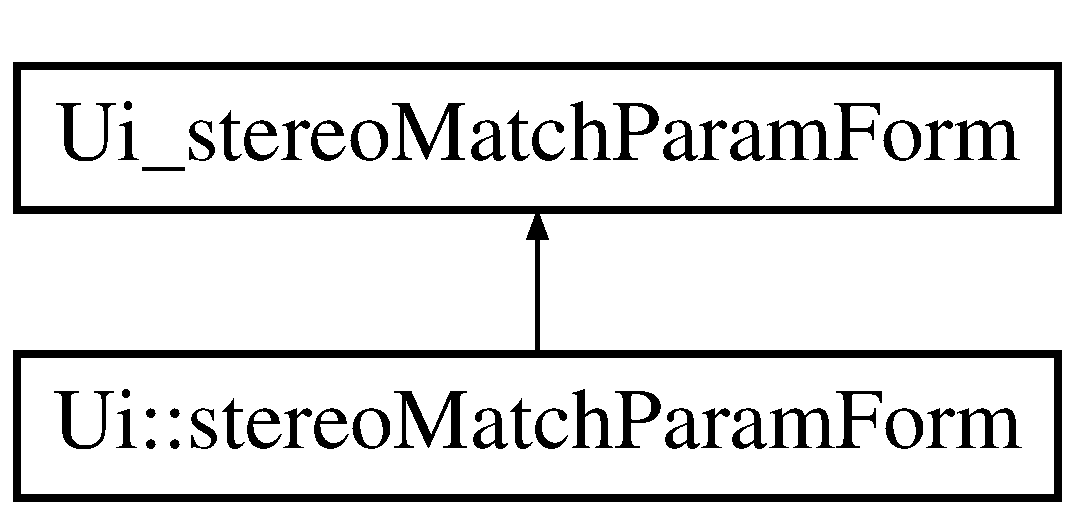
\includegraphics[height=2.000000cm]{class_ui_1_1stereo_match_param_form}
\end{center}
\end{figure}
\subsection*{Additional Inherited Members}


The documentation for this class was generated from the following file\+:\begin{DoxyCompactItemize}
\item 
D\+:/\+Qt\+Program/\+Qt5/\+Fusion/ui\+\_\+stereomatchparamform.\+h\end{DoxyCompactItemize}

\hypertarget{classstereo_match_param_form}{}\section{stereo\+Match\+Param\+Form Class Reference}
\label{classstereo_match_param_form}\index{stereo\+Match\+Param\+Form@{stereo\+Match\+Param\+Form}}
Inheritance diagram for stereo\+Match\+Param\+Form\+:\begin{figure}[H]
\begin{center}
\leavevmode
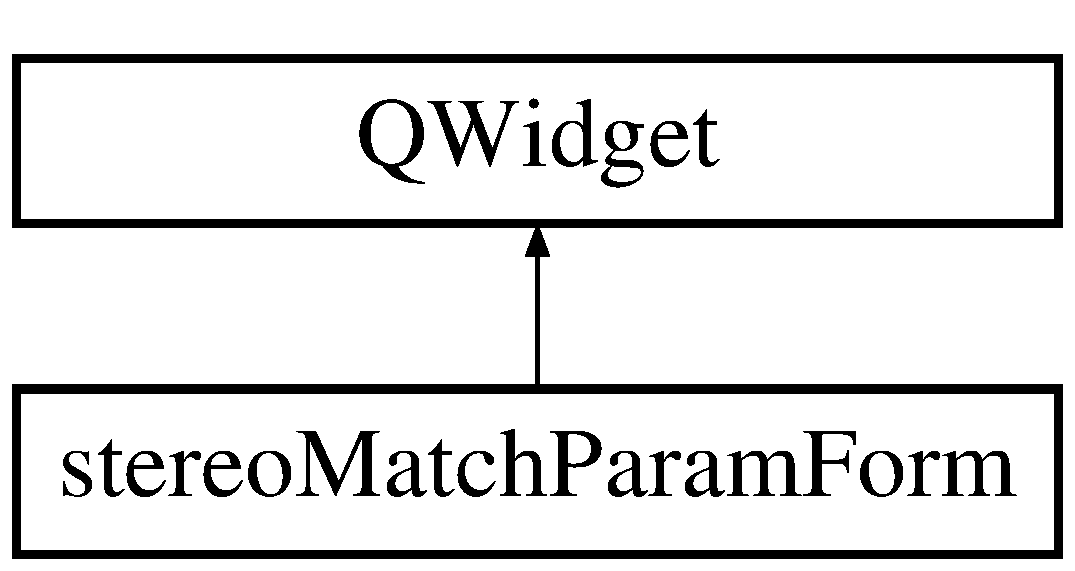
\includegraphics[height=2.000000cm]{classstereo_match_param_form}
\end{center}
\end{figure}
\subsection*{Signals}
\begin{DoxyCompactItemize}
\item 
\hypertarget{classstereo_match_param_form_af74acd5ac2278ab32913a108598c90bd}{}void {\bfseries closed} (void)\label{classstereo_match_param_form_af74acd5ac2278ab32913a108598c90bd}

\item 
\hypertarget{classstereo_match_param_form_a03eada5faaf2eab6e9a42f7234d92d7d}{}void {\bfseries send\+\_\+bm\+\_\+pre\+\_\+filter\+\_\+size} (int value)\label{classstereo_match_param_form_a03eada5faaf2eab6e9a42f7234d92d7d}

\item 
\hypertarget{classstereo_match_param_form_adb4aa9b2c117dbbf8afeeaac9d65915c}{}void {\bfseries send\+\_\+bm\+\_\+pre\+\_\+filter\+\_\+cap} (int value)\label{classstereo_match_param_form_adb4aa9b2c117dbbf8afeeaac9d65915c}

\item 
\hypertarget{classstereo_match_param_form_a58688d07ecca1a803a14565a5ce70acd}{}void {\bfseries send\+\_\+bm\+\_\+sad\+\_\+window\+\_\+size} (int value)\label{classstereo_match_param_form_a58688d07ecca1a803a14565a5ce70acd}

\item 
\hypertarget{classstereo_match_param_form_a039af2fe00eacb179cb159a4246393d9}{}void {\bfseries send\+\_\+bm\+\_\+min\+\_\+disp} (int value)\label{classstereo_match_param_form_a039af2fe00eacb179cb159a4246393d9}

\item 
\hypertarget{classstereo_match_param_form_a15f1eea232d561b531b625f81567d65b}{}void {\bfseries send\+\_\+bm\+\_\+num\+\_\+of\+\_\+disp} (int value)\label{classstereo_match_param_form_a15f1eea232d561b531b625f81567d65b}

\item 
\hypertarget{classstereo_match_param_form_aa9bb10b9ecf3e2ff541269f8ce478d7c}{}void {\bfseries send\+\_\+bm\+\_\+texture\+\_\+thresh} (int value)\label{classstereo_match_param_form_aa9bb10b9ecf3e2ff541269f8ce478d7c}

\item 
\hypertarget{classstereo_match_param_form_a799a9bd22de77cd222cc9b2e03b3e3b2}{}void {\bfseries send\+\_\+bm\+\_\+uniqueness\+\_\+ratio} (int value)\label{classstereo_match_param_form_a799a9bd22de77cd222cc9b2e03b3e3b2}

\item 
\hypertarget{classstereo_match_param_form_a77996c75fa4f772b5d4341acfdd50b09}{}void {\bfseries send\+\_\+bm\+\_\+speckle\+\_\+window\+\_\+size} (int value)\label{classstereo_match_param_form_a77996c75fa4f772b5d4341acfdd50b09}

\item 
\hypertarget{classstereo_match_param_form_a2b7c372cd0d9f42c25a44d5eaf99c2ff}{}void {\bfseries send\+\_\+bm\+\_\+speckle\+\_\+range} (int value)\label{classstereo_match_param_form_a2b7c372cd0d9f42c25a44d5eaf99c2ff}

\item 
\hypertarget{classstereo_match_param_form_acd316b30cc3066f8a32032b78ff283c7}{}void {\bfseries send\+\_\+sgbm\+\_\+pre\+\_\+filter\+\_\+cap} (int value)\label{classstereo_match_param_form_acd316b30cc3066f8a32032b78ff283c7}

\item 
\hypertarget{classstereo_match_param_form_a6492eca6d362722865ab44aaf2a155fd}{}void {\bfseries send\+\_\+sgbm\+\_\+sad\+\_\+window\+\_\+size} (int value)\label{classstereo_match_param_form_a6492eca6d362722865ab44aaf2a155fd}

\item 
\hypertarget{classstereo_match_param_form_a01a9c02e35a8e68a07fe04a13b575c14}{}void {\bfseries send\+\_\+sgbm\+\_\+min\+\_\+disp} (int value)\label{classstereo_match_param_form_a01a9c02e35a8e68a07fe04a13b575c14}

\item 
\hypertarget{classstereo_match_param_form_a15e280c258f60965a7e972e6a78f84b2}{}void {\bfseries send\+\_\+sgbm\+\_\+num\+\_\+of\+\_\+disp} (int value)\label{classstereo_match_param_form_a15e280c258f60965a7e972e6a78f84b2}

\item 
\hypertarget{classstereo_match_param_form_aed4704b886213a80bd808bc6fac40eb9}{}void {\bfseries send\+\_\+sgbm\+\_\+uniqueness\+\_\+ratio} (int value)\label{classstereo_match_param_form_aed4704b886213a80bd808bc6fac40eb9}

\item 
\hypertarget{classstereo_match_param_form_a0402267190761324594d9800c5463d41}{}void {\bfseries send\+\_\+sgbm\+\_\+speckle\+\_\+window\+\_\+size} (int value)\label{classstereo_match_param_form_a0402267190761324594d9800c5463d41}

\item 
\hypertarget{classstereo_match_param_form_a8eba0d79f01d0067aa040b3c2705fe3d}{}void {\bfseries send\+\_\+sgbm\+\_\+speckle\+\_\+range} (int value)\label{classstereo_match_param_form_a8eba0d79f01d0067aa040b3c2705fe3d}

\end{DoxyCompactItemize}
\subsection*{Public Member Functions}
\begin{DoxyCompactItemize}
\item 
\hypertarget{classstereo_match_param_form_a723a09ecefd0bc51813c14ea713bf7be}{}{\bfseries stereo\+Match\+Param\+Form} (Q\+Widget $\ast$parent=0, int mode=S\+V\+::\+S\+T\+E\+R\+E\+O\+\_\+\+M\+A\+T\+C\+H\+::\+S\+G\+B\+M)\label{classstereo_match_param_form_a723a09ecefd0bc51813c14ea713bf7be}

\item 
\hypertarget{classstereo_match_param_form_a9efd57f345ef61d269bdefa8fb04cd48}{}void {\bfseries change\+Mode} (int mode)\label{classstereo_match_param_form_a9efd57f345ef61d269bdefa8fb04cd48}

\end{DoxyCompactItemize}
\subsection*{Private Slots}
\begin{DoxyCompactItemize}
\item 
\hypertarget{classstereo_match_param_form_a6fc9b3b33af491d24d667aaceccc7ac0}{}void {\bfseries on\+\_\+horizontal\+Slider\+\_\+bm\+\_\+pre\+\_\+filter\+\_\+size\+\_\+value\+Changed} (int value)\label{classstereo_match_param_form_a6fc9b3b33af491d24d667aaceccc7ac0}

\item 
\hypertarget{classstereo_match_param_form_ae333fa3bfc8a4e981a77894a5cf2b4d5}{}void {\bfseries on\+\_\+horizontal\+Slider\+\_\+bm\+\_\+pre\+\_\+filter\+\_\+cap\+\_\+value\+Changed} (int value)\label{classstereo_match_param_form_ae333fa3bfc8a4e981a77894a5cf2b4d5}

\item 
\hypertarget{classstereo_match_param_form_a05e103bb3adfab5e19a62dc3d4e27515}{}void {\bfseries on\+\_\+horizontal\+Slider\+\_\+bm\+\_\+sad\+\_\+window\+\_\+size\+\_\+value\+Changed} (int value)\label{classstereo_match_param_form_a05e103bb3adfab5e19a62dc3d4e27515}

\item 
\hypertarget{classstereo_match_param_form_ae572eeb4250fd61845d81329be03a4d7}{}void {\bfseries on\+\_\+horizontal\+Slider\+\_\+bm\+\_\+min\+\_\+disp\+\_\+value\+Changed} (int value)\label{classstereo_match_param_form_ae572eeb4250fd61845d81329be03a4d7}

\item 
\hypertarget{classstereo_match_param_form_a230fee1aee584226d74a54aad9293bb5}{}void {\bfseries on\+\_\+horizontal\+Slider\+\_\+bm\+\_\+num\+\_\+of\+\_\+disp\+\_\+value\+Changed} (int value)\label{classstereo_match_param_form_a230fee1aee584226d74a54aad9293bb5}

\item 
\hypertarget{classstereo_match_param_form_af6290918e0d98424abe2a5469be815d4}{}void {\bfseries on\+\_\+horizontal\+Slider\+\_\+bm\+\_\+texture\+\_\+thresh\+\_\+value\+Changed} (int value)\label{classstereo_match_param_form_af6290918e0d98424abe2a5469be815d4}

\item 
\hypertarget{classstereo_match_param_form_a5039e2ba6b375cbc147032b9450c842e}{}void {\bfseries on\+\_\+horizontal\+Slider\+\_\+bm\+\_\+uniqueness\+\_\+ratio\+\_\+value\+Changed} (int value)\label{classstereo_match_param_form_a5039e2ba6b375cbc147032b9450c842e}

\item 
\hypertarget{classstereo_match_param_form_a0a321f9430961264f75b6aa87f5e0573}{}void {\bfseries on\+\_\+horizontal\+Slider\+\_\+bm\+\_\+speckle\+\_\+window\+\_\+size\+\_\+value\+Changed} (int value)\label{classstereo_match_param_form_a0a321f9430961264f75b6aa87f5e0573}

\item 
\hypertarget{classstereo_match_param_form_a8fadcdd62022a5f1ff7e3873539d72ad}{}void {\bfseries on\+\_\+horizontal\+Slider\+\_\+bm\+\_\+speckle\+\_\+range\+\_\+value\+Changed} (int value)\label{classstereo_match_param_form_a8fadcdd62022a5f1ff7e3873539d72ad}

\item 
\hypertarget{classstereo_match_param_form_a2bb282b6a280ec76394205a349a966b0}{}void {\bfseries close\+Event} (Q\+Close\+Event $\ast$)\label{classstereo_match_param_form_a2bb282b6a280ec76394205a349a966b0}

\item 
\hypertarget{classstereo_match_param_form_a7f9028514c2576f8a8b7e4949de90f80}{}void {\bfseries on\+\_\+horizontal\+Slider\+\_\+sgbm\+\_\+pre\+\_\+filter\+\_\+cap\+\_\+value\+Changed} (int value)\label{classstereo_match_param_form_a7f9028514c2576f8a8b7e4949de90f80}

\item 
\hypertarget{classstereo_match_param_form_a3130e45c523de78d2256a3ee64b6cd41}{}void {\bfseries on\+\_\+horizontal\+Slider\+\_\+sgbm\+\_\+sad\+\_\+window\+\_\+size\+\_\+value\+Changed} (int value)\label{classstereo_match_param_form_a3130e45c523de78d2256a3ee64b6cd41}

\item 
\hypertarget{classstereo_match_param_form_a9a1f75337638bd4ba03e3908408ce66e}{}void {\bfseries on\+\_\+horizontal\+Slider\+\_\+sgbm\+\_\+min\+\_\+disp\+\_\+value\+Changed} (int value)\label{classstereo_match_param_form_a9a1f75337638bd4ba03e3908408ce66e}

\item 
\hypertarget{classstereo_match_param_form_acbf080edaba841fc5adfb04ffb8ae8fa}{}void {\bfseries on\+\_\+horizontal\+Slider\+\_\+sgbm\+\_\+num\+\_\+of\+\_\+disp\+\_\+value\+Changed} (int value)\label{classstereo_match_param_form_acbf080edaba841fc5adfb04ffb8ae8fa}

\item 
\hypertarget{classstereo_match_param_form_aea726b9a1a255116db326de7f8b1f847}{}void {\bfseries on\+\_\+horizontal\+Slider\+\_\+sgbm\+\_\+uniqueness\+\_\+ratio\+\_\+value\+Changed} (int value)\label{classstereo_match_param_form_aea726b9a1a255116db326de7f8b1f847}

\item 
\hypertarget{classstereo_match_param_form_ae2b3dc9e2aabef8bac2c982456d3b26a}{}void {\bfseries on\+\_\+horizontal\+Slider\+\_\+sgbm\+\_\+speckle\+\_\+window\+\_\+size\+\_\+value\+Changed} (int value)\label{classstereo_match_param_form_ae2b3dc9e2aabef8bac2c982456d3b26a}

\item 
\hypertarget{classstereo_match_param_form_a97ac246adec788de95d8a44d435e610b}{}void {\bfseries on\+\_\+horizontal\+Slider\+\_\+sgbm\+\_\+speckle\+\_\+range\+\_\+value\+Changed} (int value)\label{classstereo_match_param_form_a97ac246adec788de95d8a44d435e610b}

\item 
\hypertarget{classstereo_match_param_form_a51f43a349453d57e03693f61d8006a2a}{}void {\bfseries update\+Params} (int cur\+\_\+mode, std\+::vector$<$ int $>$ param)\label{classstereo_match_param_form_a51f43a349453d57e03693f61d8006a2a}

\end{DoxyCompactItemize}
\subsection*{Private Attributes}
\begin{DoxyCompactItemize}
\item 
\hypertarget{classstereo_match_param_form_a9d27a67d083c85f3ae2490f7344a0fd2}{}\hyperlink{class_ui_1_1stereo_match_param_form}{Ui\+::stereo\+Match\+Param\+Form} $\ast$ {\bfseries ui}\label{classstereo_match_param_form_a9d27a67d083c85f3ae2490f7344a0fd2}

\item 
\hypertarget{classstereo_match_param_form_a0225a335c88a22904bbb0cd1d305c541}{}int {\bfseries mode}\label{classstereo_match_param_form_a0225a335c88a22904bbb0cd1d305c541}

\item 
\hypertarget{classstereo_match_param_form_ae01ea10b7cb68a3e104ec20f0bf86fdd}{}bool {\bfseries fg\+\_\+sgbm\+\_\+changed}\label{classstereo_match_param_form_ae01ea10b7cb68a3e104ec20f0bf86fdd}

\item 
\hypertarget{classstereo_match_param_form_a1980626db05cb9aa6652d30540a3ccb1}{}bool {\bfseries fg\+\_\+bm\+\_\+changed}\label{classstereo_match_param_form_a1980626db05cb9aa6652d30540a3ccb1}

\end{DoxyCompactItemize}


The documentation for this class was generated from the following files\+:\begin{DoxyCompactItemize}
\item 
D\+:/\+Qt\+Program/\+Qt5/\+Fusion/stereomatchparamform.\+h\item 
D\+:/\+Qt\+Program/\+Qt5/\+Fusion/stereomatchparamform.\+cpp\end{DoxyCompactItemize}

\hypertarget{class_top_view}{}\section{Top\+View Class Reference}
\label{class_top_view}\index{Top\+View@{Top\+View}}
Inheritance diagram for Top\+View\+:\begin{figure}[H]
\begin{center}
\leavevmode
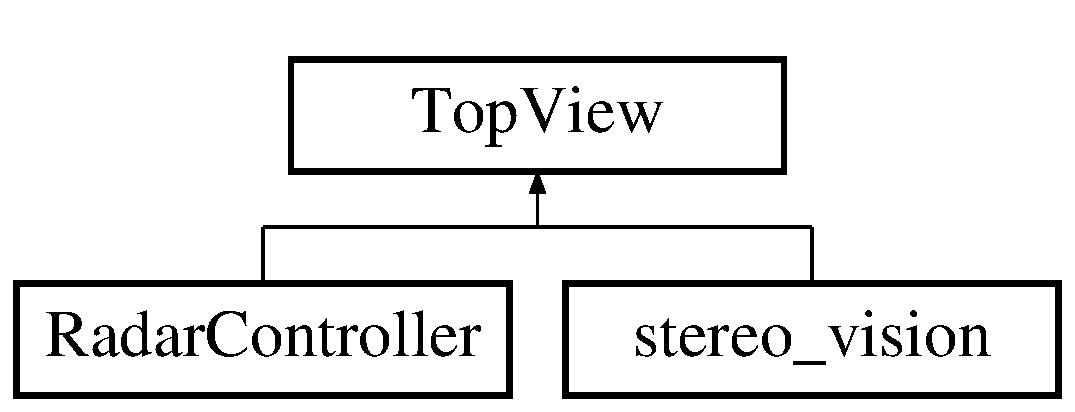
\includegraphics[height=2.000000cm]{class_top_view}
\end{center}
\end{figure}
\subsection*{Classes}
\begin{DoxyCompactItemize}
\item 
struct \hyperlink{struct_top_view_1_1blob_node}{blob\+Node}
\end{DoxyCompactItemize}
\subsection*{Public Member Functions}
\begin{DoxyCompactItemize}
\item 
\hypertarget{class_top_view_a7bf56ae4f4ee2cf40dafd6a82707a281}{}{\bfseries Top\+View} (int \hyperlink{class_top_view_a0be83119f0e81bbfd89f75b6d271eb2b}{thresh\+\_\+free\+\_\+space}, int \hyperlink{class_top_view_a56c819ab3208d77a4b6f9dff80339524}{min\+\_\+distance}, int \hyperlink{class_top_view_a4d6987318631da634e6121bc563d5bfb}{max\+\_\+distance}, float \hyperlink{class_top_view_a1ad1a34440fcfb86672427e97b03870b}{view\+\_\+angle}, int \hyperlink{class_top_view_a7b492b7926c48542bdad6610a602eadc}{chord\+\_\+length}, int display\+\_\+row, int display\+\_\+col, int grid\+\_\+row, int grid\+\_\+col)\label{class_top_view_a7bf56ae4f4ee2cf40dafd6a82707a281}

\item 
\hypertarget{class_top_view_a565c1500b449240cd16bf9bdbb7ea96e}{}void {\bfseries initial\+Top\+View} ()\label{class_top_view_a565c1500b449240cd16bf9bdbb7ea96e}

\item 
\hypertarget{class_top_view_a3a88db97144313b0f8c42fb07dc20468}{}void {\bfseries draw\+Top\+View\+Lines} (int rows\+\_\+interval, int cols\+\_\+interval, bool fg\+\_\+tag)\label{class_top_view_a3a88db97144313b0f8c42fb07dc20468}

\item 
\hypertarget{class_top_view_ab3c9e49395d1ce23367c8668164549c1}{}bool {\bfseries is\+Initialized\+Top\+View} ()\label{class_top_view_ab3c9e49395d1ce23367c8668164549c1}

\item 
\hypertarget{class_top_view_aa9ec86935067642bced8bc202e5a3b7c}{}virtual void {\bfseries point\+Project\+Top\+View} ()\label{class_top_view_aa9ec86935067642bced8bc202e5a3b7c}

\item 
\hypertarget{class_top_view_ace2839bba9b0a4602a841a5794ab249c}{}void {\bfseries change\+Params} (float \hyperlink{class_top_view_a1ad1a34440fcfb86672427e97b03870b}{view\+\_\+angle}, int \hyperlink{class_top_view_a7b492b7926c48542bdad6610a602eadc}{chord\+\_\+length})\label{class_top_view_ace2839bba9b0a4602a841a5794ab249c}

\item 
\hypertarget{class_top_view_a4d1f8c93ed36cabd27c8e7d51c29c62d}{}cv\+::\+Point \hyperlink{class_top_view_a4d1f8c93ed36cabd27c8e7d51c29c62d}{point\+T} (cv\+::\+Point src)\label{class_top_view_a4d1f8c93ed36cabd27c8e7d51c29c62d}

\begin{DoxyCompactList}\small\item\em transformed point from grid map to topview for display \end{DoxyCompactList}\end{DoxyCompactItemize}
\subsection*{Public Attributes}
\begin{DoxyCompactItemize}
\item 
\hypertarget{class_top_view_a56c819ab3208d77a4b6f9dff80339524}{}int \hyperlink{class_top_view_a56c819ab3208d77a4b6f9dff80339524}{min\+\_\+distance}\label{class_top_view_a56c819ab3208d77a4b6f9dff80339524}

\begin{DoxyCompactList}\small\item\em (cm) \end{DoxyCompactList}\item 
\hypertarget{class_top_view_a4d6987318631da634e6121bc563d5bfb}{}int \hyperlink{class_top_view_a4d6987318631da634e6121bc563d5bfb}{max\+\_\+distance}\label{class_top_view_a4d6987318631da634e6121bc563d5bfb}

\begin{DoxyCompactList}\small\item\em (cm) \end{DoxyCompactList}\item 
\hypertarget{class_top_view_a1ad1a34440fcfb86672427e97b03870b}{}float \hyperlink{class_top_view_a1ad1a34440fcfb86672427e97b03870b}{view\+\_\+angle}\label{class_top_view_a1ad1a34440fcfb86672427e97b03870b}

\begin{DoxyCompactList}\small\item\em the view angle (degree) \end{DoxyCompactList}\item 
\hypertarget{class_top_view_ab5e6ef291472c707f5f4f51cd7d582a7}{}float \hyperlink{class_top_view_ab5e6ef291472c707f5f4f51cd7d582a7}{c}\label{class_top_view_ab5e6ef291472c707f5f4f51cd7d582a7}

\begin{DoxyCompactList}\small\item\em ratio of image to grid\+\_\+map (the number of adjacent image columns grouped into a polar slice) \end{DoxyCompactList}\item 
\hypertarget{class_top_view_a693454cfb21851b389634e28bdabe35a}{}cv\+::\+Mat \hyperlink{class_top_view_a693454cfb21851b389634e28bdabe35a}{topview}\label{class_top_view_a693454cfb21851b389634e28bdabe35a}

\begin{DoxyCompactList}\small\item\em topview on label \end{DoxyCompactList}\item 
\hypertarget{class_top_view_ab069be29953bc5f8e29d0799b44b6e43}{}cv\+::\+Mat {\bfseries topview\+\_\+\+B\+G}\label{class_top_view_ab069be29953bc5f8e29d0799b44b6e43}

\item 
\hypertarget{class_top_view_a6a41c281c60a67bdceca7a33abe805a5}{}Q\+Image $\ast$ {\bfseries color\+\_\+table}\label{class_top_view_a6a41c281c60a67bdceca7a33abe805a5}

\item 
\hypertarget{class_top_view_a08bac944fb14eb668817d322a1956f3b}{}cv\+::\+Scalar {\bfseries color\+\_\+\+B\+G}\label{class_top_view_a08bac944fb14eb668817d322a1956f3b}

\item 
\hypertarget{class_top_view_ac0094dc43998e987ff269e93263f6983}{}cv\+::\+Scalar {\bfseries color\+\_\+tag}\label{class_top_view_ac0094dc43998e987ff269e93263f6983}

\item 
\hypertarget{class_top_view_a1eac41f96e88d30801e1b813ac97a111}{}cv\+::\+Scalar {\bfseries color\+\_\+line}\label{class_top_view_a1eac41f96e88d30801e1b813ac97a111}

\end{DoxyCompactItemize}
\subsection*{Protected Member Functions}
\begin{DoxyCompactItemize}
\item 
\hypertarget{class_top_view_a13003b4bba4ddbf745ee7b9611e70cdb}{}void {\bfseries reset\+Top\+View} ()\label{class_top_view_a13003b4bba4ddbf745ee7b9611e70cdb}

\end{DoxyCompactItemize}
\subsection*{Protected Attributes}
\begin{DoxyCompactItemize}
\item 
\hypertarget{class_top_view_a4aa887937748785f2b1f80039397e0e4}{}int {\bfseries thick\+\_\+polygon}\label{class_top_view_a4aa887937748785f2b1f80039397e0e4}

\item 
\hypertarget{class_top_view_ad62ba0fd78ab35b854a4ee101904d449}{}int {\bfseries img\+\_\+col}\label{class_top_view_ad62ba0fd78ab35b854a4ee101904d449}

\item 
\hypertarget{class_top_view_a39648976b29089f0d8b95504e5a35d06}{}int {\bfseries img\+\_\+col\+\_\+half}\label{class_top_view_a39648976b29089f0d8b95504e5a35d06}

\item 
\hypertarget{class_top_view_a4e9b5eaf65fdb222fac5d2aa40940611}{}int {\bfseries img\+\_\+row}\label{class_top_view_a4e9b5eaf65fdb222fac5d2aa40940611}

\item 
\hypertarget{class_top_view_a97556995e814b8072cde301fe4443384}{}float \hyperlink{class_top_view_a97556995e814b8072cde301fe4443384}{ratio\+\_\+row}\label{class_top_view_a97556995e814b8072cde301fe4443384}

\begin{DoxyCompactList}\small\item\em ratio of display\+\_\+row to max\+\_\+distance \end{DoxyCompactList}\item 
\hypertarget{class_top_view_a13a5f7ab64db7898b53055e4ac65d266}{}float \hyperlink{class_top_view_a13a5f7ab64db7898b53055e4ac65d266}{ratio\+\_\+col}\label{class_top_view_a13a5f7ab64db7898b53055e4ac65d266}

\begin{DoxyCompactList}\small\item\em ratio of display\+\_\+col to chord\+\_\+length \end{DoxyCompactList}\item 
\hypertarget{class_top_view_a21a67bc4d0af8dd26996c6fb007aa3b4}{}int {\bfseries display\+\_\+row}\label{class_top_view_a21a67bc4d0af8dd26996c6fb007aa3b4}

\item 
\hypertarget{class_top_view_a18630cd4f3e2d76e8c5ddc687b54d098}{}int {\bfseries display\+\_\+col}\label{class_top_view_a18630cd4f3e2d76e8c5ddc687b54d098}

\item 
\hypertarget{class_top_view_a54a832929e3763160213c25f0a543128}{}\hyperlink{struct_top_view_1_1blob_node}{blob\+Node} $\ast$$\ast$ \hyperlink{class_top_view_a54a832929e3763160213c25f0a543128}{grid\+\_\+map}\label{class_top_view_a54a832929e3763160213c25f0a543128}

\begin{DoxyCompactList}\small\item\em Storing pixels\textquotesingle{} information into cells. \end{DoxyCompactList}\item 
\hypertarget{class_top_view_a72de1afcef91e63df47886fc162da3f6}{}cv\+::\+Point $\ast$$\ast$ \hyperlink{class_top_view_a72de1afcef91e63df47886fc162da3f6}{img\+\_\+grid}\label{class_top_view_a72de1afcef91e63df47886fc162da3f6}

\begin{DoxyCompactList}\small\item\em topview background cell points \end{DoxyCompactList}\item 
\hypertarget{class_top_view_a1f2b530e7979db621630dbbf9f5def15}{}float \hyperlink{class_top_view_a1f2b530e7979db621630dbbf9f5def15}{k}\label{class_top_view_a1f2b530e7979db621630dbbf9f5def15}

\begin{DoxyCompactList}\small\item\em length of interval \end{DoxyCompactList}\item 
\hypertarget{class_top_view_a7b492b7926c48542bdad6610a602eadc}{}int \hyperlink{class_top_view_a7b492b7926c48542bdad6610a602eadc}{chord\+\_\+length}\label{class_top_view_a7b492b7926c48542bdad6610a602eadc}

\begin{DoxyCompactList}\small\item\em the chord length of stereo vision \end{DoxyCompactList}\item 
\hypertarget{class_top_view_ab5a42f3e0ca928ea973c052c538ba354}{}int \hyperlink{class_top_view_ab5a42f3e0ca928ea973c052c538ba354}{chord\+\_\+length\+\_\+min}\label{class_top_view_ab5a42f3e0ca928ea973c052c538ba354}

\begin{DoxyCompactList}\small\item\em the chord length at min\+\_\+distance \end{DoxyCompactList}\item 
\hypertarget{class_top_view_a0be83119f0e81bbfd89f75b6d271eb2b}{}int \hyperlink{class_top_view_a0be83119f0e81bbfd89f75b6d271eb2b}{thresh\+\_\+free\+\_\+space}\label{class_top_view_a0be83119f0e81bbfd89f75b6d271eb2b}

\begin{DoxyCompactList}\small\item\em check whether the cell is satisfied as an object.~\newline
 Each cell containing more than this value is consider as an object. \end{DoxyCompactList}\end{DoxyCompactItemize}
\subsection*{Private Member Functions}
\begin{DoxyCompactItemize}
\item 
\hypertarget{class_top_view_a56698a690e0107a9c5fc7bb7740b47fe}{}void {\bfseries release\+Top\+View} ()\label{class_top_view_a56698a690e0107a9c5fc7bb7740b47fe}

\item 
\hypertarget{class_top_view_a63a2c70756e7f4fd5f86000091a1c51b}{}void {\bfseries pseudo\+Color\+Table} ()\label{class_top_view_a63a2c70756e7f4fd5f86000091a1c51b}

\end{DoxyCompactItemize}
\subsection*{Private Attributes}
\begin{DoxyCompactItemize}
\item 
\hypertarget{class_top_view_ad38788eb0cf2dc43399a4f7d85d62c52}{}bool \hyperlink{class_top_view_ad38788eb0cf2dc43399a4f7d85d62c52}{fg\+\_\+topview}\label{class_top_view_ad38788eb0cf2dc43399a4f7d85d62c52}

\begin{DoxyCompactList}\small\item\em whether topview is initialized \end{DoxyCompactList}\end{DoxyCompactItemize}


The documentation for this class was generated from the following files\+:\begin{DoxyCompactItemize}
\item 
D\+:/\+Qt\+Program/\+Qt5/\+Fusion/topview.\+h\item 
D\+:/\+Qt\+Program/\+Qt5/\+Fusion/topview.\+cpp\end{DoxyCompactItemize}

\hypertarget{class_ui__calibration_form}{}\section{Ui\+\_\+calibration\+Form Class Reference}
\label{class_ui__calibration_form}\index{Ui\+\_\+calibration\+Form@{Ui\+\_\+calibration\+Form}}
Inheritance diagram for Ui\+\_\+calibration\+Form\+:\begin{figure}[H]
\begin{center}
\leavevmode
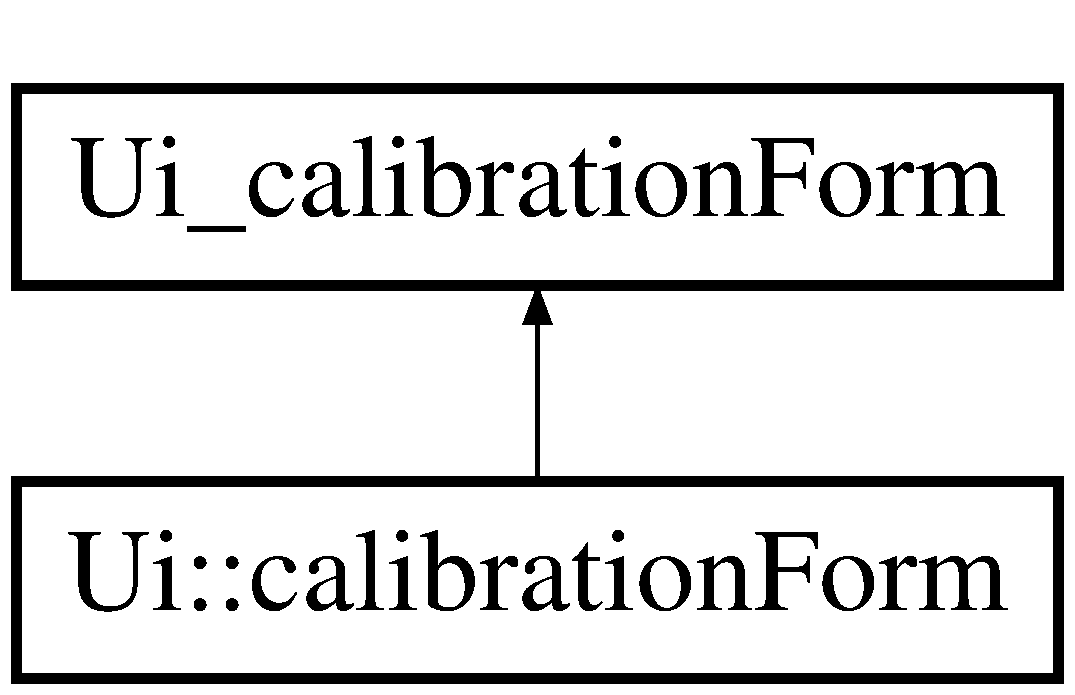
\includegraphics[height=2.000000cm]{class_ui__calibration_form}
\end{center}
\end{figure}
\subsection*{Public Member Functions}
\begin{DoxyCompactItemize}
\item 
\hypertarget{class_ui__calibration_form_ab284aff5632f3cba8f1c3d4e0437aacc}{}void {\bfseries setup\+Ui} (Q\+Widget $\ast$\hyperlink{classcalibration_form}{calibration\+Form})\label{class_ui__calibration_form_ab284aff5632f3cba8f1c3d4e0437aacc}

\item 
\hypertarget{class_ui__calibration_form_af92e3883ecb47c35e0254006b42ad50a}{}void {\bfseries retranslate\+Ui} (Q\+Widget $\ast$\hyperlink{classcalibration_form}{calibration\+Form})\label{class_ui__calibration_form_af92e3883ecb47c35e0254006b42ad50a}

\end{DoxyCompactItemize}
\subsection*{Public Attributes}
\begin{DoxyCompactItemize}
\item 
\hypertarget{class_ui__calibration_form_afabfc3a9836bfa156e3e1a559d79c41c}{}Q\+Widget $\ast$ {\bfseries layout\+Widget\+\_\+3}\label{class_ui__calibration_form_afabfc3a9836bfa156e3e1a559d79c41c}

\item 
\hypertarget{class_ui__calibration_form_aa83ed3b5715d355ee3ae25a4aa808a30}{}Q\+Form\+Layout $\ast$ {\bfseries form\+Layout}\label{class_ui__calibration_form_aa83ed3b5715d355ee3ae25a4aa808a30}

\item 
\hypertarget{class_ui__calibration_form_a3b0d0447114500d726a3f1f241825d3f}{}Q\+Label $\ast$ {\bfseries label\+\_\+3}\label{class_ui__calibration_form_a3b0d0447114500d726a3f1f241825d3f}

\item 
\hypertarget{class_ui__calibration_form_ad9842e2256ba11ec50c59a25da401d6f}{}Q\+Label $\ast$ {\bfseries label\+\_\+6}\label{class_ui__calibration_form_ad9842e2256ba11ec50c59a25da401d6f}

\item 
\hypertarget{class_ui__calibration_form_a9f174c8ecf7c5e6111cf1a18f406522f}{}Q\+Label $\ast$ {\bfseries label\+\_\+recorded\+L}\label{class_ui__calibration_form_a9f174c8ecf7c5e6111cf1a18f406522f}

\item 
\hypertarget{class_ui__calibration_form_aca78a0150881ca3965fd1b5831accbff}{}Q\+Label $\ast$ {\bfseries label\+\_\+recorded\+R}\label{class_ui__calibration_form_aca78a0150881ca3965fd1b5831accbff}

\item 
\hypertarget{class_ui__calibration_form_a37c11d4701454f67747c77bb367b0e2c}{}Q\+Label $\ast$ {\bfseries label\+\_\+7}\label{class_ui__calibration_form_a37c11d4701454f67747c77bb367b0e2c}

\item 
\hypertarget{class_ui__calibration_form_a9a5eecb0f712ac42d73a6078b217b521}{}Q\+Widget $\ast$ {\bfseries layout\+Widget}\label{class_ui__calibration_form_a9a5eecb0f712ac42d73a6078b217b521}

\item 
\hypertarget{class_ui__calibration_form_ad74f2cc0fd516b9736d849ea2bd2e88e}{}Q\+Grid\+Layout $\ast$ {\bfseries grid\+Layout}\label{class_ui__calibration_form_ad74f2cc0fd516b9736d849ea2bd2e88e}

\item 
\hypertarget{class_ui__calibration_form_af6369a3359bfca1891ea0e86db122fd2}{}Q\+Grid\+Layout $\ast$ {\bfseries grid\+Layout\+\_\+2}\label{class_ui__calibration_form_af6369a3359bfca1891ea0e86db122fd2}

\item 
\hypertarget{class_ui__calibration_form_a1edc1349bafbe5225f7f5437fe197541}{}Q\+Label $\ast$ {\bfseries label\+\_\+8}\label{class_ui__calibration_form_a1edc1349bafbe5225f7f5437fe197541}

\item 
\hypertarget{class_ui__calibration_form_ab551d3deba9b2ffba6947f47c5ab848b}{}Q\+Label $\ast$ {\bfseries label\+\_\+4}\label{class_ui__calibration_form_ab551d3deba9b2ffba6947f47c5ab848b}

\item 
\hypertarget{class_ui__calibration_form_ac1e5b0e1a23e5c08b1f08de7a6019ca5}{}Q\+Line\+Edit $\ast$ {\bfseries line\+Edit\+\_\+grid\+\_\+w}\label{class_ui__calibration_form_ac1e5b0e1a23e5c08b1f08de7a6019ca5}

\item 
\hypertarget{class_ui__calibration_form_a9bbd69b321ebc9dbec915f65e73d6bc2}{}Q\+Label $\ast$ {\bfseries label\+\_\+5}\label{class_ui__calibration_form_a9bbd69b321ebc9dbec915f65e73d6bc2}

\item 
\hypertarget{class_ui__calibration_form_ae7305784fc046a84123757dbf929a360}{}Q\+Line\+Edit $\ast$ {\bfseries line\+Edit\+\_\+grid\+\_\+h}\label{class_ui__calibration_form_ae7305784fc046a84123757dbf929a360}

\item 
\hypertarget{class_ui__calibration_form_acabd3ba7dd8c0c406dac9d280fd15022}{}Q\+Grid\+Layout $\ast$ {\bfseries grid\+Layout\+\_\+3}\label{class_ui__calibration_form_acabd3ba7dd8c0c406dac9d280fd15022}

\item 
\hypertarget{class_ui__calibration_form_a320b08d1c7f6bdb4ca5f44285cf3c4ba}{}Q\+Label $\ast$ {\bfseries label\+\_\+9}\label{class_ui__calibration_form_a320b08d1c7f6bdb4ca5f44285cf3c4ba}

\item 
\hypertarget{class_ui__calibration_form_a61bb7523ad103edf7f99f514bdb611eb}{}Q\+Label $\ast$ {\bfseries label\+\_\+10}\label{class_ui__calibration_form_a61bb7523ad103edf7f99f514bdb611eb}

\item 
\hypertarget{class_ui__calibration_form_a8d45977518e4bfe0e65cde011d572f16}{}Q\+Spin\+Box $\ast$ {\bfseries spin\+Box\+\_\+corners\+\_\+cols}\label{class_ui__calibration_form_a8d45977518e4bfe0e65cde011d572f16}

\item 
\hypertarget{class_ui__calibration_form_a5f1613c55ba70f5d798e6c5b08c89b45}{}Q\+Spin\+Box $\ast$ {\bfseries spin\+Box\+\_\+corners\+\_\+rows}\label{class_ui__calibration_form_a5f1613c55ba70f5d798e6c5b08c89b45}

\item 
\hypertarget{class_ui__calibration_form_a3f2fecb9aaf40cab405f381f3a8ec1de}{}Q\+Spacer\+Item $\ast$ {\bfseries horizontal\+Spacer}\label{class_ui__calibration_form_a3f2fecb9aaf40cab405f381f3a8ec1de}

\item 
\hypertarget{class_ui__calibration_form_a358c84164c30246387591d2c21246bb7}{}Q\+Label $\ast$ {\bfseries label\+\_\+11}\label{class_ui__calibration_form_a358c84164c30246387591d2c21246bb7}

\item 
\hypertarget{class_ui__calibration_form_a78391f3438e253d7700092a530bcf30d}{}Q\+Push\+Button $\ast$ {\bfseries push\+Button\+\_\+calibration}\label{class_ui__calibration_form_a78391f3438e253d7700092a530bcf30d}

\item 
\hypertarget{class_ui__calibration_form_a4925459341f6593e26156ccc401421ad}{}Q\+Push\+Button $\ast$ {\bfseries push\+Button\+\_\+3}\label{class_ui__calibration_form_a4925459341f6593e26156ccc401421ad}

\item 
\hypertarget{class_ui__calibration_form_a8b775bb32c33a7db877b842d302455de}{}Q\+Check\+Box $\ast$ {\bfseries check\+Box\+\_\+\+Save\+Both}\label{class_ui__calibration_form_a8b775bb32c33a7db877b842d302455de}

\item 
\hypertarget{class_ui__calibration_form_a69a40d8f1c5455676702edde2f374163}{}Q\+Label $\ast$ {\bfseries label\+\_\+status}\label{class_ui__calibration_form_a69a40d8f1c5455676702edde2f374163}

\item 
\hypertarget{class_ui__calibration_form_a3b0ea8f3c42bf5f5365aa10e54cbc295}{}Q\+Push\+Button $\ast$ {\bfseries push\+Button\+\_\+corner\+\_\+intrinsic}\label{class_ui__calibration_form_a3b0ea8f3c42bf5f5365aa10e54cbc295}

\item 
\hypertarget{class_ui__calibration_form_ac8f817c5b55ec50f17f9c48d6e8cf2f3}{}Q\+Progress\+Bar $\ast$ {\bfseries progress\+Bar}\label{class_ui__calibration_form_ac8f817c5b55ec50f17f9c48d6e8cf2f3}

\end{DoxyCompactItemize}


The documentation for this class was generated from the following file\+:\begin{DoxyCompactItemize}
\item 
D\+:/\+Qt\+Program/\+Qt5/\+Fusion/ui\+\_\+calibrationform.\+h\end{DoxyCompactItemize}

\hypertarget{class_ui___main_window}{}\section{Ui\+\_\+\+Main\+Window Class Reference}
\label{class_ui___main_window}\index{Ui\+\_\+\+Main\+Window@{Ui\+\_\+\+Main\+Window}}
Inheritance diagram for Ui\+\_\+\+Main\+Window\+:\begin{figure}[H]
\begin{center}
\leavevmode
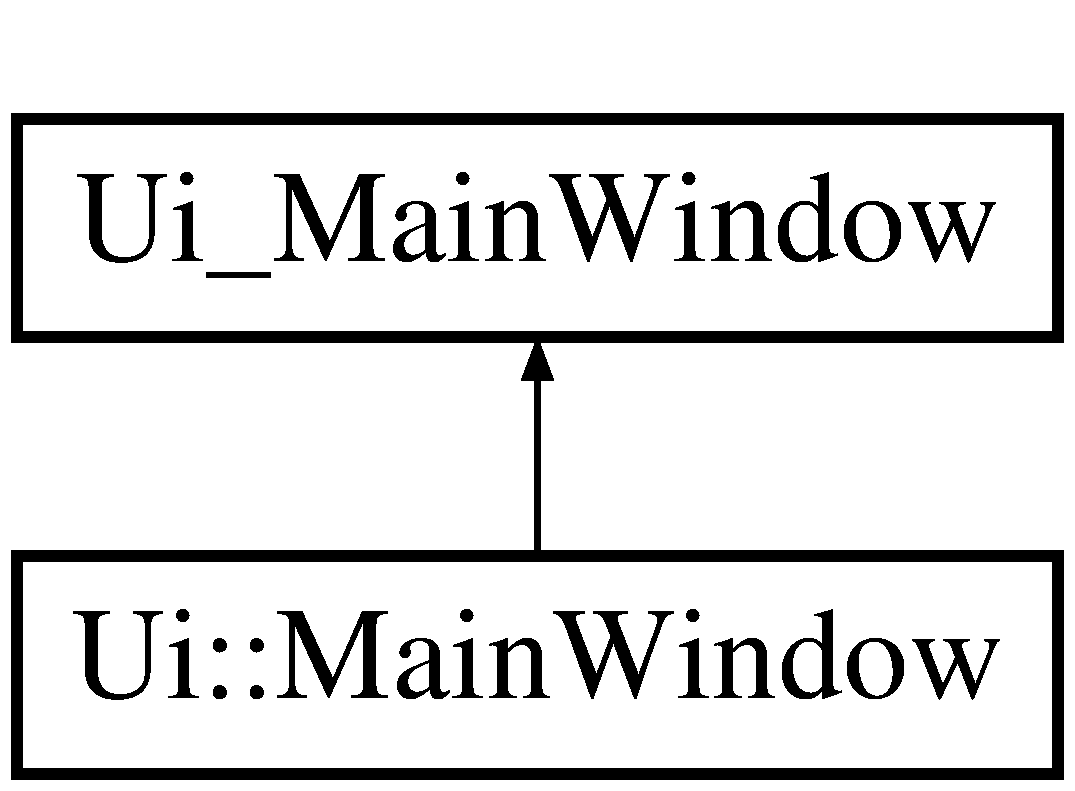
\includegraphics[height=2.000000cm]{class_ui___main_window}
\end{center}
\end{figure}
\subsection*{Public Member Functions}
\begin{DoxyCompactItemize}
\item 
\hypertarget{class_ui___main_window_acf4a0872c4c77d8f43a2ec66ed849b58}{}void {\bfseries setup\+Ui} (Q\+Main\+Window $\ast$\hyperlink{class_main_window}{Main\+Window})\label{class_ui___main_window_acf4a0872c4c77d8f43a2ec66ed849b58}

\item 
\hypertarget{class_ui___main_window_a097dd160c3534a204904cb374412c618}{}void {\bfseries retranslate\+Ui} (Q\+Main\+Window $\ast$\hyperlink{class_main_window}{Main\+Window})\label{class_ui___main_window_a097dd160c3534a204904cb374412c618}

\end{DoxyCompactItemize}
\subsection*{Public Attributes}
\begin{DoxyCompactItemize}
\item 
\hypertarget{class_ui___main_window_adc1a970564dde02b162f66db0495114d}{}Q\+Action $\ast$ {\bfseries action\+Shortcut}\label{class_ui___main_window_adc1a970564dde02b162f66db0495114d}

\item 
\hypertarget{class_ui___main_window_a5a231f47d88c3b71593d5766acb72ce6}{}Q\+Action $\ast$ {\bfseries action\+Author}\label{class_ui___main_window_a5a231f47d88c3b71593d5766acb72ce6}

\item 
\hypertarget{class_ui___main_window_a30075506c2116c3ed4ff25e07ae75f81}{}Q\+Widget $\ast$ {\bfseries central\+Widget}\label{class_ui___main_window_a30075506c2116c3ed4ff25e07ae75f81}

\item 
\hypertarget{class_ui___main_window_a3260b943854b841c986f47c4726ee7f9}{}Q\+Tab\+Widget $\ast$ {\bfseries tab\+Widget}\label{class_ui___main_window_a3260b943854b841c986f47c4726ee7f9}

\item 
\hypertarget{class_ui___main_window_a3efc28c664e9f5115095aafbbc5ac6bc}{}Q\+Widget $\ast$ {\bfseries tab}\label{class_ui___main_window_a3efc28c664e9f5115095aafbbc5ac6bc}

\item 
\hypertarget{class_ui___main_window_a098e217ec87c740d62b047d2bc0137ad}{}Q\+Push\+Button $\ast$ {\bfseries push\+Button\+\_\+lrf\+\_\+open}\label{class_ui___main_window_a098e217ec87c740d62b047d2bc0137ad}

\item 
\hypertarget{class_ui___main_window_ab96ab0f0578098521fa69a75aa5cdde8}{}Q\+Widget $\ast$ {\bfseries layout\+Widget}\label{class_ui___main_window_ab96ab0f0578098521fa69a75aa5cdde8}

\item 
\hypertarget{class_ui___main_window_a525ed3c5fe0784ac502ee222fba4e205}{}Q\+Grid\+Layout $\ast$ {\bfseries grid\+Layout}\label{class_ui___main_window_a525ed3c5fe0784ac502ee222fba4e205}

\item 
\hypertarget{class_ui___main_window_ad9c89133780f28e6efa2ec17ceb9cff5}{}Q\+Label $\ast$ {\bfseries label}\label{class_ui___main_window_ad9c89133780f28e6efa2ec17ceb9cff5}

\item 
\hypertarget{class_ui___main_window_a2e2516d755e4dd53fc905dabddf2738a}{}Q\+Label $\ast$ {\bfseries label\+\_\+2}\label{class_ui___main_window_a2e2516d755e4dd53fc905dabddf2738a}

\item 
\hypertarget{class_ui___main_window_a67b26eb96863ddea8f96f5711eec2b85}{}Q\+Combo\+Box $\ast$ {\bfseries combo\+Box\+\_\+lrf\+\_\+com}\label{class_ui___main_window_a67b26eb96863ddea8f96f5711eec2b85}

\item 
\hypertarget{class_ui___main_window_a5d3f4747e662e55f1bc8ff6e6d0029ca}{}Q\+Combo\+Box $\ast$ {\bfseries combo\+Box\+\_\+lrf\+\_\+baud\+Rate}\label{class_ui___main_window_a5d3f4747e662e55f1bc8ff6e6d0029ca}

\item 
\hypertarget{class_ui___main_window_aab31b3dec8d767525dea6f163e029e48}{}Q\+Widget $\ast$ {\bfseries layout\+Widget1}\label{class_ui___main_window_aab31b3dec8d767525dea6f163e029e48}

\item 
\hypertarget{class_ui___main_window_af42ea7d4c2e893181caad21e28166932}{}Q\+Grid\+Layout $\ast$ {\bfseries grid\+Layout\+\_\+3}\label{class_ui___main_window_af42ea7d4c2e893181caad21e28166932}

\item 
\hypertarget{class_ui___main_window_a84fcb366bdfd4438dac9870225183220}{}Q\+Spin\+Box $\ast$ {\bfseries spin\+Box\+\_\+lrf\+\_\+scale}\label{class_ui___main_window_a84fcb366bdfd4438dac9870225183220}

\item 
\hypertarget{class_ui___main_window_a78c7e10730b43c6700cd7216911ed76a}{}Q\+Label $\ast$ {\bfseries label\+\_\+4}\label{class_ui___main_window_a78c7e10730b43c6700cd7216911ed76a}

\item 
\hypertarget{class_ui___main_window_a6cda85bb4cf776930c0f4d4dcf906751}{}Q\+Widget $\ast$ {\bfseries layout\+Widget2}\label{class_ui___main_window_a6cda85bb4cf776930c0f4d4dcf906751}

\item 
\hypertarget{class_ui___main_window_a8ee86315639f324b17708efc7dbe8b19}{}Q\+Grid\+Layout $\ast$ {\bfseries grid\+Layout\+\_\+4}\label{class_ui___main_window_a8ee86315639f324b17708efc7dbe8b19}

\item 
\hypertarget{class_ui___main_window_acaecd1db33f9aa13dba05c3d8eed664e}{}Q\+Radio\+Button $\ast$ {\bfseries radio\+Button\+\_\+lrf\+\_\+res\+\_\+cm}\label{class_ui___main_window_acaecd1db33f9aa13dba05c3d8eed664e}

\item 
\hypertarget{class_ui___main_window_ac5371e73462a4e7982e20a31984209c0}{}Q\+Radio\+Button $\ast$ {\bfseries radio\+Button\+\_\+lrf\+\_\+res\+\_\+mm}\label{class_ui___main_window_ac5371e73462a4e7982e20a31984209c0}

\item 
\hypertarget{class_ui___main_window_ad6bab8fb8903b8f41afea1218ee52695}{}Q\+Label $\ast$ {\bfseries label\+\_\+5}\label{class_ui___main_window_ad6bab8fb8903b8f41afea1218ee52695}

\item 
\hypertarget{class_ui___main_window_a17cbf43ae5323e4121225f483c2f2824}{}Q\+Widget $\ast$ {\bfseries layout\+Widget3}\label{class_ui___main_window_a17cbf43ae5323e4121225f483c2f2824}

\item 
\hypertarget{class_ui___main_window_adbbd44debcfc24db144006951bf7b3e1}{}Q\+Grid\+Layout $\ast$ {\bfseries grid\+Layout\+\_\+12}\label{class_ui___main_window_adbbd44debcfc24db144006951bf7b3e1}

\item 
\hypertarget{class_ui___main_window_a7a9350c6de61e7051850744487d910bd}{}Q\+Label $\ast$ {\bfseries label\+\_\+23}\label{class_ui___main_window_a7a9350c6de61e7051850744487d910bd}

\item 
\hypertarget{class_ui___main_window_ad3f0ee52c147bb9e62086b990e429fee}{}Q\+Push\+Button $\ast$ {\bfseries push\+Button\+\_\+lrf\+\_\+request\+\_\+2}\label{class_ui___main_window_ad3f0ee52c147bb9e62086b990e429fee}

\item 
\hypertarget{class_ui___main_window_a7fcb1f46747d4b0e5bbd5cb72e932312}{}Q\+Push\+Button $\ast$ {\bfseries push\+Button\+\_\+lrf\+\_\+retrieve\+\_\+2}\label{class_ui___main_window_a7fcb1f46747d4b0e5bbd5cb72e932312}

\item 
\hypertarget{class_ui___main_window_acfb77433cf941396a64f41d4fada7bb0}{}Q\+Push\+Button $\ast$ {\bfseries push\+Button\+\_\+lrf\+\_\+stop\+\_\+2}\label{class_ui___main_window_acfb77433cf941396a64f41d4fada7bb0}

\item 
\hypertarget{class_ui___main_window_a6697c4b75a94a17e8cc5f78a7b6b785d}{}Q\+Widget $\ast$ {\bfseries layout\+Widget4}\label{class_ui___main_window_a6697c4b75a94a17e8cc5f78a7b6b785d}

\item 
\hypertarget{class_ui___main_window_a16419b7fa6d38eb8c34d4a937c5d8ecd}{}Q\+Grid\+Layout $\ast$ {\bfseries grid\+Layout\+\_\+13}\label{class_ui___main_window_a16419b7fa6d38eb8c34d4a937c5d8ecd}

\item 
\hypertarget{class_ui___main_window_a5aaa4a7aebd23f957bba2ba79b581839}{}Q\+Push\+Button $\ast$ {\bfseries push\+Button\+\_\+lrf\+\_\+request\+\_\+\+O\+N\+C\+E}\label{class_ui___main_window_a5aaa4a7aebd23f957bba2ba79b581839}

\item 
\hypertarget{class_ui___main_window_aec4a1b9f3a28cdaf5a58c9e2da46bd9a}{}Q\+Push\+Button $\ast$ {\bfseries push\+Button\+\_\+lrf\+\_\+stop}\label{class_ui___main_window_aec4a1b9f3a28cdaf5a58c9e2da46bd9a}

\item 
\hypertarget{class_ui___main_window_aa9f87a074a15b824af87132c5fa8e640}{}Q\+Push\+Button $\ast$ {\bfseries push\+Button\+\_\+lrf\+\_\+retrieve}\label{class_ui___main_window_aa9f87a074a15b824af87132c5fa8e640}

\item 
\hypertarget{class_ui___main_window_a738324b6c2ace1b7534ff0da28bc3eff}{}Q\+Push\+Button $\ast$ {\bfseries push\+Button\+\_\+lrf\+\_\+request}\label{class_ui___main_window_a738324b6c2ace1b7534ff0da28bc3eff}

\item 
\hypertarget{class_ui___main_window_a83495b23cbc6810f81978dc0d584b810}{}Q\+Widget $\ast$ {\bfseries tab\+\_\+2}\label{class_ui___main_window_a83495b23cbc6810f81978dc0d584b810}

\item 
\hypertarget{class_ui___main_window_a873441ec9cec68e0d4eacee271765553}{}Q\+Widget $\ast$ {\bfseries layout\+Widget\+\_\+2}\label{class_ui___main_window_a873441ec9cec68e0d4eacee271765553}

\item 
\hypertarget{class_ui___main_window_a8731b71c513ff94baf59614807823c5d}{}Q\+Grid\+Layout $\ast$ {\bfseries grid\+Layout\+\_\+5}\label{class_ui___main_window_a8731b71c513ff94baf59614807823c5d}

\item 
\hypertarget{class_ui___main_window_a13936e6f18b1c90402b3c7a3c92b6cdb}{}Q\+Label $\ast$ {\bfseries label\+\_\+7}\label{class_ui___main_window_a13936e6f18b1c90402b3c7a3c92b6cdb}

\item 
\hypertarget{class_ui___main_window_ac4807cadb1f6e308826f513a4b0ec292}{}Q\+Combo\+Box $\ast$ {\bfseries combo\+Box\+\_\+cam\+\_\+device\+\_\+index\+\_\+\+R}\label{class_ui___main_window_ac4807cadb1f6e308826f513a4b0ec292}

\item 
\hypertarget{class_ui___main_window_a9665eedf3f4d4e253d92e1dc0581bcd7}{}Q\+Combo\+Box $\ast$ {\bfseries combo\+Box\+\_\+cam\+\_\+device\+\_\+index\+\_\+\+L}\label{class_ui___main_window_a9665eedf3f4d4e253d92e1dc0581bcd7}

\item 
\hypertarget{class_ui___main_window_a9dc4dba26b83e0c94aa566e1c564420b}{}Q\+Label $\ast$ {\bfseries label\+\_\+10}\label{class_ui___main_window_a9dc4dba26b83e0c94aa566e1c564420b}

\item 
\hypertarget{class_ui___main_window_abd7a23e5ef5692a6c53a6f47538afcd5}{}Q\+Line\+Edit $\ast$ {\bfseries line\+Edit\+\_\+base\+\_\+line}\label{class_ui___main_window_abd7a23e5ef5692a6c53a6f47538afcd5}

\item 
\hypertarget{class_ui___main_window_af183bfbfb9f38bbdd60caf92b15e23dc}{}Q\+Label $\ast$ {\bfseries label\+\_\+8}\label{class_ui___main_window_af183bfbfb9f38bbdd60caf92b15e23dc}

\item 
\hypertarget{class_ui___main_window_a663f728e6244926a795c6e6892673b1d}{}Q\+Label $\ast$ {\bfseries label\+\_\+6}\label{class_ui___main_window_a663f728e6244926a795c6e6892673b1d}

\item 
\hypertarget{class_ui___main_window_a89cb298a28a58f568d8048b38733ff3b}{}Q\+Line\+Edit $\ast$ {\bfseries line\+Edit\+\_\+sv\+\_\+rig\+\_\+height}\label{class_ui___main_window_a89cb298a28a58f568d8048b38733ff3b}

\item 
\hypertarget{class_ui___main_window_a4640e3039f2d34e4deb39787925c7d37}{}Q\+Label $\ast$ {\bfseries label\+\_\+43}\label{class_ui___main_window_a4640e3039f2d34e4deb39787925c7d37}

\item 
\hypertarget{class_ui___main_window_a6118b996a4f85be44e94bd62d74df158}{}Q\+Label $\ast$ {\bfseries label\+\_\+sv\+\_\+rig\+\_\+height}\label{class_ui___main_window_a6118b996a4f85be44e94bd62d74df158}

\item 
\hypertarget{class_ui___main_window_abac129cd2a98ad7ea6084617bdd09c82}{}Q\+Push\+Button $\ast$ {\bfseries push\+Button\+\_\+cam\+\_\+open}\label{class_ui___main_window_abac129cd2a98ad7ea6084617bdd09c82}

\item 
\hypertarget{class_ui___main_window_abdce8dd1f86488df9778d1e0c30d607f}{}Q\+Push\+Button $\ast$ {\bfseries push\+Button\+\_\+cam\+\_\+stop}\label{class_ui___main_window_abdce8dd1f86488df9778d1e0c30d607f}

\item 
\hypertarget{class_ui___main_window_a65af8477c0dde07ecd7a9d01cd145bc4}{}Q\+Push\+Button $\ast$ {\bfseries push\+Button\+\_\+cam\+\_\+step}\label{class_ui___main_window_a65af8477c0dde07ecd7a9d01cd145bc4}

\item 
\hypertarget{class_ui___main_window_a65b3c0470d73019b73f13912ce874c60}{}Q\+Push\+Button $\ast$ {\bfseries push\+Button\+\_\+cam\+\_\+capture}\label{class_ui___main_window_a65b3c0470d73019b73f13912ce874c60}

\item 
\hypertarget{class_ui___main_window_a200124ca7d59a2a338363af2942846a6}{}Q\+Widget $\ast$ {\bfseries layout\+Widget5}\label{class_ui___main_window_a200124ca7d59a2a338363af2942846a6}

\item 
\hypertarget{class_ui___main_window_a20728ed83bf740332bd908ea3e15ace6}{}Q\+Grid\+Layout $\ast$ {\bfseries grid\+Layout\+\_\+8}\label{class_ui___main_window_a20728ed83bf740332bd908ea3e15ace6}

\item 
\hypertarget{class_ui___main_window_a4f12a71b4a2fb6f85df2300d83b5ed3e}{}Q\+Label $\ast$ {\bfseries label\+\_\+11}\label{class_ui___main_window_a4f12a71b4a2fb6f85df2300d83b5ed3e}

\item 
\hypertarget{class_ui___main_window_ac88bc8d5e17fa05a6230e3076fe1d790}{}Q\+Radio\+Button $\ast$ {\bfseries radio\+Button\+\_\+\+B\+M}\label{class_ui___main_window_ac88bc8d5e17fa05a6230e3076fe1d790}

\item 
\hypertarget{class_ui___main_window_a6ca62514eb7192249d849988595747c9}{}Q\+Radio\+Button $\ast$ {\bfseries radio\+Button\+\_\+\+S\+G\+B\+M}\label{class_ui___main_window_a6ca62514eb7192249d849988595747c9}

\item 
\hypertarget{class_ui___main_window_a7504e7aa409886f0d6f577a9c305d88e}{}Q\+Push\+Button $\ast$ {\bfseries push\+Button\+\_\+camera\+\_\+calibration}\label{class_ui___main_window_a7504e7aa409886f0d6f577a9c305d88e}

\item 
\hypertarget{class_ui___main_window_a6ba9fbb2c327428701160f7ec43fc3d3}{}Q\+Push\+Button $\ast$ {\bfseries push\+Button\+\_\+stereo\+\_\+match\+\_\+param}\label{class_ui___main_window_a6ba9fbb2c327428701160f7ec43fc3d3}

\item 
\hypertarget{class_ui___main_window_a7a9ee0fe03def9f5fa802288651af9b4}{}Q\+Widget $\ast$ {\bfseries layout\+Widget6}\label{class_ui___main_window_a7a9ee0fe03def9f5fa802288651af9b4}

\item 
\hypertarget{class_ui___main_window_a1f91d05a063890efd359caac0338c7b0}{}Q\+Grid\+Layout $\ast$ {\bfseries grid\+Layout\+\_\+17}\label{class_ui___main_window_a1f91d05a063890efd359caac0338c7b0}

\item 
\hypertarget{class_ui___main_window_ae35071328d0668a7e62e047029368bed}{}Q\+Check\+Box $\ast$ {\bfseries check\+Box\+\_\+do\+\_\+depth}\label{class_ui___main_window_ae35071328d0668a7e62e047029368bed}

\item 
\hypertarget{class_ui___main_window_af670c1897b37e4093073974f3bbf7c09}{}Q\+Check\+Box $\ast$ {\bfseries check\+Box\+\_\+do\+\_\+calibration}\label{class_ui___main_window_af670c1897b37e4093073974f3bbf7c09}

\item 
\hypertarget{class_ui___main_window_a1fc06a178397ef63d25fe96349099ab8}{}Q\+Check\+Box $\ast$ {\bfseries check\+Box\+\_\+sv\+\_\+topview}\label{class_ui___main_window_a1fc06a178397ef63d25fe96349099ab8}

\item 
\hypertarget{class_ui___main_window_aedebdae38e5446839b1f1f2983f69a54}{}Q\+Check\+Box $\ast$ {\bfseries check\+Box\+\_\+sv\+\_\+reproject}\label{class_ui___main_window_aedebdae38e5446839b1f1f2983f69a54}

\item 
\hypertarget{class_ui___main_window_aab0c094f66a7f74c317e9eb2e7689911}{}Q\+Check\+Box $\ast$ {\bfseries check\+Box\+\_\+sv\+\_\+ground\+\_\+filter}\label{class_ui___main_window_aab0c094f66a7f74c317e9eb2e7689911}

\item 
\hypertarget{class_ui___main_window_ae5e48c20d3d248c796e55fcba3ea2ba2}{}Q\+Check\+Box $\ast$ {\bfseries check\+Box\+\_\+pseudo\+\_\+color}\label{class_ui___main_window_ae5e48c20d3d248c796e55fcba3ea2ba2}

\item 
\hypertarget{class_ui___main_window_ad24fd0169d0cc3ed51496d31e547a70b}{}Q\+Check\+Box $\ast$ {\bfseries check\+Box\+\_\+sv\+\_\+matching}\label{class_ui___main_window_ad24fd0169d0cc3ed51496d31e547a70b}

\item 
\hypertarget{class_ui___main_window_a5010b4398d1ab2848f0d321919cc35bb}{}Q\+Widget $\ast$ {\bfseries grid\+Layout\+Widget\+\_\+10}\label{class_ui___main_window_a5010b4398d1ab2848f0d321919cc35bb}

\item 
\hypertarget{class_ui___main_window_a82eb42bdbffbbd70131d0f615609aa71}{}Q\+Grid\+Layout $\ast$ {\bfseries grid\+Layout\+\_\+15}\label{class_ui___main_window_a82eb42bdbffbbd70131d0f615609aa71}

\item 
\hypertarget{class_ui___main_window_a8110ede36f3bb3b9940f23c99ed25ce0}{}Q\+Spin\+Box $\ast$ {\bfseries spin\+Box\+\_\+topview\+\_\+c}\label{class_ui___main_window_a8110ede36f3bb3b9940f23c99ed25ce0}

\item 
\hypertarget{class_ui___main_window_ab433b6488e9c02ce6e08480ab94d1e36}{}Q\+Spin\+Box $\ast$ {\bfseries spin\+Box\+\_\+topview\+\_\+r}\label{class_ui___main_window_ab433b6488e9c02ce6e08480ab94d1e36}

\item 
\hypertarget{class_ui___main_window_a1bf8f5e6531b7bc79378d58ee57ba389}{}Q\+Label $\ast$ {\bfseries label\+\_\+26}\label{class_ui___main_window_a1bf8f5e6531b7bc79378d58ee57ba389}

\item 
\hypertarget{class_ui___main_window_acf6fc9bce4db154fecbd1ff532918353}{}Q\+Label $\ast$ {\bfseries label\+\_\+25}\label{class_ui___main_window_acf6fc9bce4db154fecbd1ff532918353}

\item 
\hypertarget{class_ui___main_window_a31fc1e3e6c2d61c1dc50e96b6a60344d}{}Q\+Label $\ast$ {\bfseries label\+\_\+28}\label{class_ui___main_window_a31fc1e3e6c2d61c1dc50e96b6a60344d}

\item 
\hypertarget{class_ui___main_window_a33dd6998309a6bf6037295e3d07f2371}{}Q\+Check\+Box $\ast$ {\bfseries check\+Box\+\_\+topview\+\_\+plot\+\_\+points}\label{class_ui___main_window_a33dd6998309a6bf6037295e3d07f2371}

\item 
\hypertarget{class_ui___main_window_ac6c19d112b25073d9276c377d00dbadb}{}Q\+Label $\ast$ {\bfseries label\+\_\+27}\label{class_ui___main_window_ac6c19d112b25073d9276c377d00dbadb}

\item 
\hypertarget{class_ui___main_window_adae4a47910c32af51c19161423e88618}{}Q\+Widget $\ast$ {\bfseries layout\+Widget7}\label{class_ui___main_window_adae4a47910c32af51c19161423e88618}

\item 
\hypertarget{class_ui___main_window_a2bb984d720e889f05d38dac3cf7949c9}{}Q\+Grid\+Layout $\ast$ {\bfseries grid\+Layout\+\_\+21}\label{class_ui___main_window_a2bb984d720e889f05d38dac3cf7949c9}

\item 
\hypertarget{class_ui___main_window_a4c2d544352d423a361b8ab2e1d5636ec}{}Q\+Grid\+Layout $\ast$ {\bfseries grid\+Layout\+\_\+7}\label{class_ui___main_window_a4c2d544352d423a361b8ab2e1d5636ec}

\item 
\hypertarget{class_ui___main_window_a3b3e389cb1c556a500f92e1ba63cd021}{}Q\+Combo\+Box $\ast$ {\bfseries combo\+Box\+\_\+camera\+\_\+focal\+\_\+length}\label{class_ui___main_window_a3b3e389cb1c556a500f92e1ba63cd021}

\item 
\hypertarget{class_ui___main_window_a0e90c7e9ad77386881e0b264ddb9dd22}{}Q\+Label $\ast$ {\bfseries label\+\_\+9}\label{class_ui___main_window_a0e90c7e9ad77386881e0b264ddb9dd22}

\item 
\hypertarget{class_ui___main_window_a79b264e6945e3b94a511427b1c270dd7}{}Q\+Grid\+Layout $\ast$ {\bfseries grid\+Layout\+\_\+10}\label{class_ui___main_window_a79b264e6945e3b94a511427b1c270dd7}

\item 
\hypertarget{class_ui___main_window_ab6ac4329a89041f557332f6569d94493}{}Q\+Label $\ast$ {\bfseries label\+\_\+16}\label{class_ui___main_window_ab6ac4329a89041f557332f6569d94493}

\item 
\hypertarget{class_ui___main_window_ae921883b67fcf5e8863e06d44209cebb}{}Q\+Line\+Edit $\ast$ {\bfseries line\+Edit\+\_\+sv\+\_\+focal\+\_\+length}\label{class_ui___main_window_ae921883b67fcf5e8863e06d44209cebb}

\item 
\hypertarget{class_ui___main_window_ac9c95f02d5a1526633c68b6b42af0e3c}{}Q\+Label $\ast$ {\bfseries label\+\_\+sv\+\_\+focal\+\_\+length}\label{class_ui___main_window_ac9c95f02d5a1526633c68b6b42af0e3c}

\item 
\hypertarget{class_ui___main_window_a7d8a29446578759800fab35c698b6be2}{}Q\+Widget $\ast$ {\bfseries tab\+\_\+4}\label{class_ui___main_window_a7d8a29446578759800fab35c698b6be2}

\item 
\hypertarget{class_ui___main_window_a67ec284dc24ae45cf5724cfd3714e34b}{}Q\+Push\+Button $\ast$ {\bfseries push\+Button\+\_\+radar\+\_\+open}\label{class_ui___main_window_a67ec284dc24ae45cf5724cfd3714e34b}

\item 
\hypertarget{class_ui___main_window_a9487af156e57a64fea171cf47a8e9b6f}{}Q\+Push\+Button $\ast$ {\bfseries push\+Button\+\_\+radar\+\_\+write}\label{class_ui___main_window_a9487af156e57a64fea171cf47a8e9b6f}

\item 
\hypertarget{class_ui___main_window_ac34893c399af195cf5567ab86921f749}{}Q\+Push\+Button $\ast$ {\bfseries push\+Button\+\_\+radar\+\_\+bus\+\_\+on}\label{class_ui___main_window_ac34893c399af195cf5567ab86921f749}

\item 
\hypertarget{class_ui___main_window_ada00708af0ef7d93c2dd8e480ae2bdfc}{}Q\+Push\+Button $\ast$ {\bfseries push\+Button\+\_\+radar\+\_\+bus\+\_\+off}\label{class_ui___main_window_ada00708af0ef7d93c2dd8e480ae2bdfc}

\item 
\hypertarget{class_ui___main_window_aecb176939acf82378803b4ce8e8e07b6}{}Q\+Check\+Box $\ast$ {\bfseries check\+Box\+\_\+radar\+\_\+topview}\label{class_ui___main_window_aecb176939acf82378803b4ce8e8e07b6}

\item 
\hypertarget{class_ui___main_window_ae092907e20623373b790789a01756d3d}{}Q\+Widget $\ast$ {\bfseries grid\+Layout\+Widget\+\_\+11}\label{class_ui___main_window_ae092907e20623373b790789a01756d3d}

\item 
\hypertarget{class_ui___main_window_a1482572d55e80324ebb4a9e53c0120e3}{}Q\+Grid\+Layout $\ast$ {\bfseries grid\+Layout\+\_\+16}\label{class_ui___main_window_a1482572d55e80324ebb4a9e53c0120e3}

\item 
\hypertarget{class_ui___main_window_a6f531d3f4695065311f1be6faecefac7}{}Q\+Spin\+Box $\ast$ {\bfseries spin\+Box\+\_\+radar\+\_\+topview\+\_\+c}\label{class_ui___main_window_a6f531d3f4695065311f1be6faecefac7}

\item 
\hypertarget{class_ui___main_window_a42f43a5485d4938125a9feb5a3a8d4af}{}Q\+Spin\+Box $\ast$ {\bfseries spin\+Box\+\_\+radar\+\_\+topview\+\_\+r}\label{class_ui___main_window_a42f43a5485d4938125a9feb5a3a8d4af}

\item 
\hypertarget{class_ui___main_window_aa0d07c96f36b94e35e584256ee6b6d9e}{}Q\+Label $\ast$ {\bfseries label\+\_\+32}\label{class_ui___main_window_aa0d07c96f36b94e35e584256ee6b6d9e}

\item 
\hypertarget{class_ui___main_window_a92ada1ca7f65b72ecf4cba1198c44380}{}Q\+Label $\ast$ {\bfseries label\+\_\+33}\label{class_ui___main_window_a92ada1ca7f65b72ecf4cba1198c44380}

\item 
\hypertarget{class_ui___main_window_ad8951142a7b5408cf5f0f3b10c79a1a4}{}Q\+Label $\ast$ {\bfseries label\+\_\+30}\label{class_ui___main_window_ad8951142a7b5408cf5f0f3b10c79a1a4}

\item 
\hypertarget{class_ui___main_window_a40eea22fe5c81f370b7464d2e962fe8d}{}Q\+Label $\ast$ {\bfseries label\+\_\+31}\label{class_ui___main_window_a40eea22fe5c81f370b7464d2e962fe8d}

\item 
\hypertarget{class_ui___main_window_aef8650db0d2b71afdbb1abc0194dd8c4}{}Q\+Push\+Button $\ast$ {\bfseries push\+Button\+\_\+radar\+\_\+step}\label{class_ui___main_window_aef8650db0d2b71afdbb1abc0194dd8c4}

\item 
\hypertarget{class_ui___main_window_a41c7e77dd12b9445e13dbe8fb5ae1488}{}Q\+Widget $\ast$ {\bfseries tab\+\_\+3}\label{class_ui___main_window_a41c7e77dd12b9445e13dbe8fb5ae1488}

\item 
\hypertarget{class_ui___main_window_aef7cb3be8cecfc9aaf98f036a98781ce}{}Q\+Group\+Box $\ast$ {\bfseries group\+Box}\label{class_ui___main_window_aef7cb3be8cecfc9aaf98f036a98781ce}

\item 
\hypertarget{class_ui___main_window_a11715b413537235bc73b0f013c334d3b}{}Q\+Widget $\ast$ {\bfseries layout\+Widget8}\label{class_ui___main_window_a11715b413537235bc73b0f013c334d3b}

\item 
\hypertarget{class_ui___main_window_a4495f53e7dd496615426ada2042c051b}{}Q\+Grid\+Layout $\ast$ {\bfseries grid\+Layout\+\_\+14}\label{class_ui___main_window_a4495f53e7dd496615426ada2042c051b}

\item 
\hypertarget{class_ui___main_window_a29b781f23566d0f91b217459c06929ba}{}Q\+Label $\ast$ {\bfseries label\+\_\+24}\label{class_ui___main_window_a29b781f23566d0f91b217459c06929ba}

\item 
\hypertarget{class_ui___main_window_ae0d25af9b3ed9386441e76f06d3f3ddb}{}Q\+Slider $\ast$ {\bfseries horizontal\+Slider}\label{class_ui___main_window_ae0d25af9b3ed9386441e76f06d3f3ddb}

\item 
\hypertarget{class_ui___main_window_a7d1e73d93735ae30872e496b475bd45b}{}Q\+Slider $\ast$ {\bfseries horizontal\+Slider\+\_\+2}\label{class_ui___main_window_a7d1e73d93735ae30872e496b475bd45b}

\item 
\hypertarget{class_ui___main_window_adf73d4c9dedf503c14d35d44c57e169e}{}Q\+Push\+Button $\ast$ {\bfseries push\+Button\+\_\+sv\+\_\+read\+\_\+images}\label{class_ui___main_window_adf73d4c9dedf503c14d35d44c57e169e}

\item 
\hypertarget{class_ui___main_window_a2ac5fbe45a889e1ae917b7276b20bd1c}{}Q\+Push\+Button $\ast$ {\bfseries push\+Button\+\_\+sv\+\_\+read\+\_\+disp}\label{class_ui___main_window_a2ac5fbe45a889e1ae917b7276b20bd1c}

\item 
\hypertarget{class_ui___main_window_a95524248505587a7437e8428cd7d807a}{}Q\+Push\+Button $\ast$ {\bfseries push\+Button\+\_\+sv\+\_\+record\+\_\+data}\label{class_ui___main_window_a95524248505587a7437e8428cd7d807a}

\item 
\hypertarget{class_ui___main_window_a3d489698de6864b27fdecfbc7c4e266e}{}Q\+Push\+Button $\ast$ {\bfseries push\+Button\+\_\+lrf\+\_\+read\+\_\+range}\label{class_ui___main_window_a3d489698de6864b27fdecfbc7c4e266e}

\item 
\hypertarget{class_ui___main_window_ae8965af479ad55109b7d84c2010f7b24}{}Q\+Push\+Button $\ast$ {\bfseries push\+Button\+\_\+lrf\+\_\+read\+\_\+range\+\_\+2}\label{class_ui___main_window_ae8965af479ad55109b7d84c2010f7b24}

\item 
\hypertarget{class_ui___main_window_a46366f6ce04245d968218717ff8b91ab}{}Q\+Widget $\ast$ {\bfseries layout\+Widget9}\label{class_ui___main_window_a46366f6ce04245d968218717ff8b91ab}

\item 
\hypertarget{class_ui___main_window_a0bdc0d6ee9d3d95f58c53d84871f82b9}{}Q\+Grid\+Layout $\ast$ {\bfseries grid\+Layout\+\_\+11}\label{class_ui___main_window_a0bdc0d6ee9d3d95f58c53d84871f82b9}

\item 
\hypertarget{class_ui___main_window_a55100f53189f25cf8a1ee0beb29be642}{}Q\+Label $\ast$ {\bfseries label\+\_\+18}\label{class_ui___main_window_a55100f53189f25cf8a1ee0beb29be642}

\item 
\hypertarget{class_ui___main_window_a2319c1b7290c1b0736f43d613646a51e}{}Q\+Push\+Button $\ast$ {\bfseries push\+Button\+\_\+lrf\+\_\+record\+\_\+data}\label{class_ui___main_window_a2319c1b7290c1b0736f43d613646a51e}

\item 
\hypertarget{class_ui___main_window_ac59a31d0746689ef20d1d3891f162488}{}Q\+Push\+Button $\ast$ {\bfseries push\+Button\+\_\+lrf\+\_\+record\+\_\+stop}\label{class_ui___main_window_ac59a31d0746689ef20d1d3891f162488}

\item 
\hypertarget{class_ui___main_window_abb28acde35ffce4d0e6152579df2cbc3}{}Q\+Group\+Box $\ast$ {\bfseries group\+Box\+\_\+2}\label{class_ui___main_window_abb28acde35ffce4d0e6152579df2cbc3}

\item 
\hypertarget{class_ui___main_window_ac6075c1c562a25c8a858ee58fc57c140}{}Q\+Slider $\ast$ {\bfseries horizontal\+Slider\+\_\+ana\+\_\+range\+\_\+filter\+\_\+min}\label{class_ui___main_window_ac6075c1c562a25c8a858ee58fc57c140}

\item 
\hypertarget{class_ui___main_window_aeaa664b636e02543a3047acb6d8918c5}{}Q\+L\+C\+D\+Number $\ast$ {\bfseries lcd\+Number}\label{class_ui___main_window_aeaa664b636e02543a3047acb6d8918c5}

\item 
\hypertarget{class_ui___main_window_aa58070a08b061548ea4b4ec9a45101f8}{}Q\+L\+C\+D\+Number $\ast$ {\bfseries lcd\+Number\+\_\+2}\label{class_ui___main_window_aa58070a08b061548ea4b4ec9a45101f8}

\item 
\hypertarget{class_ui___main_window_a86b9e6ad43954d0e353e7c9c362c39b6}{}Q\+Slider $\ast$ {\bfseries horizontal\+Slider\+\_\+ana\+\_\+range\+\_\+filter\+\_\+max}\label{class_ui___main_window_a86b9e6ad43954d0e353e7c9c362c39b6}

\item 
\hypertarget{class_ui___main_window_abddd01ee40763254b283264c3d2cc992}{}Q\+Check\+Box $\ast$ {\bfseries check\+Box\+\_\+display\+\_\+literature\+\_\+mode}\label{class_ui___main_window_abddd01ee40763254b283264c3d2cc992}

\item 
\hypertarget{class_ui___main_window_a1c4b9067d74fe75d55c50bb96fee4061}{}Q\+Widget $\ast$ {\bfseries tab\+\_\+9}\label{class_ui___main_window_a1c4b9067d74fe75d55c50bb96fee4061}

\item 
\hypertarget{class_ui___main_window_a320d3d7ba1cb8fff7b7b95923ed10f5e}{}Q\+Group\+Box $\ast$ {\bfseries group\+Box\+\_\+3}\label{class_ui___main_window_a320d3d7ba1cb8fff7b7b95923ed10f5e}

\item 
\hypertarget{class_ui___main_window_a64f5277417ca42fc0714dc1cf9c4dabf}{}Q\+Check\+Box $\ast$ {\bfseries check\+Box\+\_\+ot\+\_\+vel}\label{class_ui___main_window_a64f5277417ca42fc0714dc1cf9c4dabf}

\item 
\hypertarget{class_ui___main_window_a45306e34db41100fe185b74d3cc6671c}{}Q\+Check\+Box $\ast$ {\bfseries check\+Box\+\_\+ot\+\_\+pf}\label{class_ui___main_window_a45306e34db41100fe185b74d3cc6671c}

\item 
\hypertarget{class_ui___main_window_a948ac79877648de63555370f7b27bcb9}{}Q\+Check\+Box $\ast$ {\bfseries check\+Box\+\_\+ot}\label{class_ui___main_window_a948ac79877648de63555370f7b27bcb9}

\item 
\hypertarget{class_ui___main_window_a5c6d40b788691613b5bd2427cf0c7012}{}Q\+Check\+Box $\ast$ {\bfseries check\+Box\+\_\+ot\+\_\+trajectory\+\_\+kalman}\label{class_ui___main_window_a5c6d40b788691613b5bd2427cf0c7012}

\item 
\hypertarget{class_ui___main_window_a781c6e86964f1387d2f43c81d36ca9e1}{}Q\+Check\+Box $\ast$ {\bfseries check\+Box\+\_\+ot\+\_\+kf}\label{class_ui___main_window_a781c6e86964f1387d2f43c81d36ca9e1}

\item 
\hypertarget{class_ui___main_window_abf094cb2744384a6eecc2a07aef43688}{}Q\+Check\+Box $\ast$ {\bfseries check\+Box\+\_\+ot\+\_\+trajectory}\label{class_ui___main_window_abf094cb2744384a6eecc2a07aef43688}

\item 
\hypertarget{class_ui___main_window_a68d971cd3693147053b452a1c91128ac}{}Q\+Check\+Box $\ast$ {\bfseries check\+Box\+\_\+ot\+\_\+trajectory\+\_\+raw}\label{class_ui___main_window_a68d971cd3693147053b452a1c91128ac}

\item 
\hypertarget{class_ui___main_window_ad8a919e5634add9c41bfc319cb9fd338}{}Q\+Group\+Box $\ast$ {\bfseries group\+Box\+\_\+4}\label{class_ui___main_window_ad8a919e5634add9c41bfc319cb9fd338}

\item 
\hypertarget{class_ui___main_window_afa8b1c11258d1b5fbf209cdbe99805b6}{}Q\+Check\+Box $\ast$ {\bfseries check\+Box\+\_\+ca}\label{class_ui___main_window_afa8b1c11258d1b5fbf209cdbe99805b6}

\item 
\hypertarget{class_ui___main_window_a639cb67bffcd8f729df5cde0877feb51}{}Q\+Check\+Box $\ast$ {\bfseries check\+Box\+\_\+ca\+\_\+astar}\label{class_ui___main_window_a639cb67bffcd8f729df5cde0877feb51}

\item 
\hypertarget{class_ui___main_window_aa408c7e16953f8329ef35ca534377fe6}{}Q\+Check\+Box $\ast$ {\bfseries check\+Box\+\_\+ca\+\_\+vfh}\label{class_ui___main_window_aa408c7e16953f8329ef35ca534377fe6}

\item 
\hypertarget{class_ui___main_window_ac71e43c9a7d3f7dd9c4d80ad91ef3e1d}{}Q\+Widget $\ast$ {\bfseries layout\+Widget10}\label{class_ui___main_window_ac71e43c9a7d3f7dd9c4d80ad91ef3e1d}

\item 
\hypertarget{class_ui___main_window_a6b2a0c5f7e8ff2a87134908dd770d2d2}{}Q\+Grid\+Layout $\ast$ {\bfseries grid\+Layout\+\_\+2}\label{class_ui___main_window_a6b2a0c5f7e8ff2a87134908dd770d2d2}

\item 
\hypertarget{class_ui___main_window_aadf16cced30349b038d552026207501f}{}Q\+Text\+Edit $\ast$ {\bfseries system\+\_\+log}\label{class_ui___main_window_aadf16cced30349b038d552026207501f}

\item 
\hypertarget{class_ui___main_window_a0376fd90247280e7c7957cc70628708c}{}Q\+Label $\ast$ {\bfseries label\+\_\+3}\label{class_ui___main_window_a0376fd90247280e7c7957cc70628708c}

\item 
\hypertarget{class_ui___main_window_a8622a9630156d191b5e4f2d3418d9f1f}{}Q\+Tab\+Widget $\ast$ {\bfseries tab\+Widget\+\_\+display}\label{class_ui___main_window_a8622a9630156d191b5e4f2d3418d9f1f}

\item 
\hypertarget{class_ui___main_window_ade7c1b9f7cb71a865cc304772c36278f}{}Q\+Widget $\ast$ {\bfseries tab\+\_\+7}\label{class_ui___main_window_ade7c1b9f7cb71a865cc304772c36278f}

\item 
\hypertarget{class_ui___main_window_a9cc1bbeab5a602fcfb4141a20fee5a87}{}Q\+Label $\ast$ {\bfseries label\+\_\+lrf\+\_\+data}\label{class_ui___main_window_a9cc1bbeab5a602fcfb4141a20fee5a87}

\item 
\hypertarget{class_ui___main_window_aad74521e428512d48b674c6c97ff0036}{}Q\+Label $\ast$ {\bfseries label\+\_\+lrf\+\_\+data\+\_\+\+B\+G}\label{class_ui___main_window_aad74521e428512d48b674c6c97ff0036}

\item 
\hypertarget{class_ui___main_window_aa9899d9e0d47ad34988a47a9d58c9d4c}{}Q\+Widget $\ast$ {\bfseries tab\+\_\+5}\label{class_ui___main_window_aa9899d9e0d47ad34988a47a9d58c9d4c}

\item 
\hypertarget{class_ui___main_window_af4b013e5c35f4afec886a70f6110cc60}{}Q\+Label $\ast$ {\bfseries label\+\_\+color\+\_\+table}\label{class_ui___main_window_af4b013e5c35f4afec886a70f6110cc60}

\item 
\hypertarget{class_ui___main_window_a08a50f32c303654803ef812c4ea1de0b}{}Q\+Label $\ast$ {\bfseries label\+\_\+depth\+\_\+info}\label{class_ui___main_window_a08a50f32c303654803ef812c4ea1de0b}

\item 
\hypertarget{class_ui___main_window_a0cab648378ea063cfae96f00010c8191}{}Q\+Label $\ast$ {\bfseries label\+\_\+top\+\_\+view\+\_\+bg}\label{class_ui___main_window_a0cab648378ea063cfae96f00010c8191}

\item 
\hypertarget{class_ui___main_window_ad237ddfde4cbe816a36ca9a4d089bc09}{}Q\+Label $\ast$ {\bfseries label\+\_\+top\+\_\+view\+\_\+sv}\label{class_ui___main_window_ad237ddfde4cbe816a36ca9a4d089bc09}

\item 
\hypertarget{class_ui___main_window_aaff386bcb60eb8ef7f8335b5c137bb1c}{}Q\+Label $\ast$ {\bfseries label\+\_\+cam\+\_\+img\+\_\+\+R}\label{class_ui___main_window_aaff386bcb60eb8ef7f8335b5c137bb1c}

\item 
\hypertarget{class_ui___main_window_a4ee2339c013c3c08a97f4ba514ad64e4}{}\hyperlink{class_mouse_label}{Mouse\+Label} $\ast$ {\bfseries label\+\_\+disp}\label{class_ui___main_window_a4ee2339c013c3c08a97f4ba514ad64e4}

\item 
\hypertarget{class_ui___main_window_a4607060872a6e254df4f91d93b32769b}{}\hyperlink{class_mouse_label}{Mouse\+Label} $\ast$ {\bfseries label\+\_\+cam\+\_\+img\+\_\+\+L}\label{class_ui___main_window_a4607060872a6e254df4f91d93b32769b}

\item 
\hypertarget{class_ui___main_window_a59e43dded72c952e66a10ee17fb3a652}{}\hyperlink{class_mouse_label}{Mouse\+Label} $\ast$ {\bfseries label\+\_\+sv\+\_\+detected}\label{class_ui___main_window_a59e43dded72c952e66a10ee17fb3a652}

\item 
\hypertarget{class_ui___main_window_a8492f118ee3c39459c458d802fcef8af}{}Q\+Label $\ast$ {\bfseries label\+\_\+sv\+\_\+frame\+\_\+count}\label{class_ui___main_window_a8492f118ee3c39459c458d802fcef8af}

\item 
\hypertarget{class_ui___main_window_a193f7d89d896d9369f4a1173de796fd1}{}Q\+Widget $\ast$ {\bfseries tab\+\_\+6}\label{class_ui___main_window_a193f7d89d896d9369f4a1173de796fd1}

\item 
\hypertarget{class_ui___main_window_a45e03fdf49983c144b517119ac3a440b}{}Q\+Label $\ast$ {\bfseries label\+\_\+top\+\_\+view\+\_\+radar\+\_\+long}\label{class_ui___main_window_a45e03fdf49983c144b517119ac3a440b}

\item 
\hypertarget{class_ui___main_window_abdd13cb702c8cb09a43f62bf38520f9d}{}Q\+Label $\ast$ {\bfseries label\+\_\+top\+\_\+view\+\_\+radar\+\_\+long\+\_\+\+B\+G}\label{class_ui___main_window_abdd13cb702c8cb09a43f62bf38520f9d}

\item 
\hypertarget{class_ui___main_window_a42660e6c7a071d30333009eae5d33e2b}{}Q\+Label $\ast$ {\bfseries label\+\_\+radar\+\_\+data}\label{class_ui___main_window_a42660e6c7a071d30333009eae5d33e2b}

\item 
\hypertarget{class_ui___main_window_ac15eb83bc0e07682c180dce67af163db}{}Q\+Label $\ast$ {\bfseries label\+\_\+radar\+\_\+data\+\_\+\+B\+G}\label{class_ui___main_window_ac15eb83bc0e07682c180dce67af163db}

\item 
\hypertarget{class_ui___main_window_aadbe82966fc3d6fa23ed1dbf38fb8149}{}Q\+Table\+View $\ast$ {\bfseries table\+View\+\_\+radar}\label{class_ui___main_window_aadbe82966fc3d6fa23ed1dbf38fb8149}

\item 
\hypertarget{class_ui___main_window_a0e030dc0e538b74ec4887801fb73ffa8}{}Q\+Widget $\ast$ {\bfseries tab\+\_\+8}\label{class_ui___main_window_a0e030dc0e538b74ec4887801fb73ffa8}

\item 
\hypertarget{class_ui___main_window_ae056359bffda73b3db9e939804dab36e}{}Q\+Label $\ast$ {\bfseries label\+\_\+fusion\+\_\+\+B\+G}\label{class_ui___main_window_ae056359bffda73b3db9e939804dab36e}

\item 
\hypertarget{class_ui___main_window_ab1dac93b95bf5dd47e68f709cd97282f}{}Q\+Label $\ast$ {\bfseries label\+\_\+fusion}\label{class_ui___main_window_ab1dac93b95bf5dd47e68f709cd97282f}

\item 
\hypertarget{class_ui___main_window_a4a4f07e3592955089bcf3456f713ac75}{}Q\+Widget $\ast$ {\bfseries layout\+Widget11}\label{class_ui___main_window_a4a4f07e3592955089bcf3456f713ac75}

\item 
\hypertarget{class_ui___main_window_ad113cf7b76aaf178473555bdf64ff035}{}Q\+Grid\+Layout $\ast$ {\bfseries grid\+Layout\+\_\+6}\label{class_ui___main_window_ad113cf7b76aaf178473555bdf64ff035}

\item 
\hypertarget{class_ui___main_window_a3f70e2348372af055e3a2b08bccaeea6}{}Q\+Check\+Box $\ast$ {\bfseries check\+Box\+\_\+fusion\+\_\+sv}\label{class_ui___main_window_a3f70e2348372af055e3a2b08bccaeea6}

\item 
\hypertarget{class_ui___main_window_a64d371dba203240e399877aaf44b40eb}{}Q\+Label $\ast$ {\bfseries label\+\_\+fusion\+\_\+sv\+\_\+color}\label{class_ui___main_window_a64d371dba203240e399877aaf44b40eb}

\item 
\hypertarget{class_ui___main_window_a9a057c7fdf9e2336a10dc84f1302fc17}{}Q\+Check\+Box $\ast$ {\bfseries check\+Box\+\_\+fusion\+\_\+radar}\label{class_ui___main_window_a9a057c7fdf9e2336a10dc84f1302fc17}

\item 
\hypertarget{class_ui___main_window_ad9d4f69ac4a99c2baa0d7187cf147fb0}{}Q\+Label $\ast$ {\bfseries label\+\_\+fusion\+\_\+radar\+\_\+color}\label{class_ui___main_window_ad9d4f69ac4a99c2baa0d7187cf147fb0}

\item 
\hypertarget{class_ui___main_window_a7871ea8c4b6c595d7ccd53960b344719}{}Q\+Spacer\+Item $\ast$ {\bfseries horizontal\+Spacer}\label{class_ui___main_window_a7871ea8c4b6c595d7ccd53960b344719}

\item 
\hypertarget{class_ui___main_window_ab3c17036e06558f71eb8a1ecf0917201}{}Q\+Check\+Box $\ast$ {\bfseries check\+Box\+\_\+fusion\+\_\+data}\label{class_ui___main_window_ab3c17036e06558f71eb8a1ecf0917201}

\item 
\hypertarget{class_ui___main_window_a256d057081e055c1c7ed07bdac5f9b96}{}Q\+Check\+Box $\ast$ {\bfseries check\+Box\+\_\+fused\+\_\+sv\+\_\+plot\+\_\+every\+\_\+pixel}\label{class_ui___main_window_a256d057081e055c1c7ed07bdac5f9b96}

\item 
\hypertarget{class_ui___main_window_a4f1206e78dd6b0ca835fe19e13f8ee39}{}\hyperlink{class_mouse_label}{Mouse\+Label} $\ast$ {\bfseries label\+\_\+sv\+\_\+detected\+\_\+display}\label{class_ui___main_window_a4f1206e78dd6b0ca835fe19e13f8ee39}

\item 
\hypertarget{class_ui___main_window_a6ee4849e48d8a0fd6e12e68dfb98bc1d}{}Q\+Widget $\ast$ {\bfseries layout\+Widget12}\label{class_ui___main_window_a6ee4849e48d8a0fd6e12e68dfb98bc1d}

\item 
\hypertarget{class_ui___main_window_a4fc0865a2fea446b284d1db5fc111211}{}Q\+Grid\+Layout $\ast$ {\bfseries grid\+Layout\+\_\+22}\label{class_ui___main_window_a4fc0865a2fea446b284d1db5fc111211}

\item 
\hypertarget{class_ui___main_window_adbc3c1f79f70bbc17064c9dab4014504}{}Q\+Radio\+Button $\ast$ {\bfseries radio\+Button\+\_\+vehicle\+\_\+car}\label{class_ui___main_window_adbc3c1f79f70bbc17064c9dab4014504}

\item 
\hypertarget{class_ui___main_window_aef8665e39a13673201c86900cb630975}{}Q\+Radio\+Button $\ast$ {\bfseries radio\+Button\+\_\+vehicle\+\_\+cart}\label{class_ui___main_window_aef8665e39a13673201c86900cb630975}

\item 
\hypertarget{class_ui___main_window_acfd040d37bac1228078cd91fecf7b930}{}Q\+Radio\+Button $\ast$ {\bfseries radio\+Button\+\_\+vehicle\+\_\+tractor}\label{class_ui___main_window_acfd040d37bac1228078cd91fecf7b930}

\item 
\hypertarget{class_ui___main_window_a75a84e4b9296f604cd5ed0940286cb95}{}Q\+Label $\ast$ {\bfseries label\+\_\+gui\+\_\+\+B\+G}\label{class_ui___main_window_a75a84e4b9296f604cd5ed0940286cb95}

\item 
\hypertarget{class_ui___main_window_ab2ffde079981ca2a216424bad79d913f}{}Q\+Label $\ast$ {\bfseries label\+\_\+gui\+\_\+vehicle}\label{class_ui___main_window_ab2ffde079981ca2a216424bad79d913f}

\item 
\hypertarget{class_ui___main_window_a66f2a690513cfe3cb9ed682278ffcd60}{}Q\+Label $\ast$ {\bfseries label\+\_\+gui\+\_\+sign}\label{class_ui___main_window_a66f2a690513cfe3cb9ed682278ffcd60}

\item 
\hypertarget{class_ui___main_window_a2f61e5118e8b5d7070385316d466b73c}{}Q\+Label $\ast$ {\bfseries label\+\_\+gui\+\_\+approaching}\label{class_ui___main_window_a2f61e5118e8b5d7070385316d466b73c}

\item 
\hypertarget{class_ui___main_window_a775e4d4ca4bcbaa50bfd1ccdbbf34c23}{}Q\+Label $\ast$ {\bfseries label\+\_\+gui\+\_\+left\+\_\+oncoming}\label{class_ui___main_window_a775e4d4ca4bcbaa50bfd1ccdbbf34c23}

\item 
\hypertarget{class_ui___main_window_a17fc42cc0fb2adc1fa5e8cd867dde873}{}Q\+Label $\ast$ {\bfseries label\+\_\+gui\+\_\+right\+\_\+oncoming}\label{class_ui___main_window_a17fc42cc0fb2adc1fa5e8cd867dde873}

\item 
\hypertarget{class_ui___main_window_aad6abbb265ab3f9b51690819d32c1d09}{}Q\+Label $\ast$ {\bfseries label\+\_\+sv\+\_\+frame\+\_\+count\+\_\+2}\label{class_ui___main_window_aad6abbb265ab3f9b51690819d32c1d09}

\item 
\hypertarget{class_ui___main_window_ad122c20205eccfa9483c1bbba70d2393}{}Q\+Check\+Box $\ast$ {\bfseries check\+Box\+\_\+fused\+\_\+region\+\_\+display\+\_\+only}\label{class_ui___main_window_ad122c20205eccfa9483c1bbba70d2393}

\item 
\hypertarget{class_ui___main_window_a8a9479b398739afd841656f19dafca9e}{}Q\+Widget $\ast$ {\bfseries layout\+Widget13}\label{class_ui___main_window_a8a9479b398739afd841656f19dafca9e}

\item 
\hypertarget{class_ui___main_window_a63157bad53e80af9d929e38b532867a0}{}Q\+Grid\+Layout $\ast$ {\bfseries grid\+Layout\+\_\+18}\label{class_ui___main_window_a63157bad53e80af9d929e38b532867a0}

\item 
\hypertarget{class_ui___main_window_a4c8544db44765ebe65de4347d6e8bbdb}{}Q\+Push\+Button $\ast$ {\bfseries push\+Button\+\_\+sv\+\_\+load\+\_\+data}\label{class_ui___main_window_a4c8544db44765ebe65de4347d6e8bbdb}

\item 
\hypertarget{class_ui___main_window_a15df4e8368a9089c7529575836483ffa}{}Q\+Push\+Button $\ast$ {\bfseries push\+Button\+\_\+radar\+\_\+load\+\_\+data}\label{class_ui___main_window_a15df4e8368a9089c7529575836483ffa}

\item 
\hypertarget{class_ui___main_window_ac828745b1bd3c0f85df5a14bccd92bf1}{}Q\+Push\+Button $\ast$ {\bfseries push\+Button\+\_\+lrf\+\_\+load\+\_\+data}\label{class_ui___main_window_ac828745b1bd3c0f85df5a14bccd92bf1}

\item 
\hypertarget{class_ui___main_window_a910b27be17d3d149a32c839d30d7ee9c}{}Q\+Push\+Button $\ast$ {\bfseries push\+Button\+\_\+all\+\_\+load\+\_\+data}\label{class_ui___main_window_a910b27be17d3d149a32c839d30d7ee9c}

\item 
\hypertarget{class_ui___main_window_a438102703ff7e65b133ba3760663d554}{}Q\+Label $\ast$ {\bfseries label\+\_\+29}\label{class_ui___main_window_a438102703ff7e65b133ba3760663d554}

\item 
\hypertarget{class_ui___main_window_aeac219c7deb5536d53d995dc14fdfa06}{}Q\+Label $\ast$ {\bfseries label\+\_\+41}\label{class_ui___main_window_aeac219c7deb5536d53d995dc14fdfa06}

\item 
\hypertarget{class_ui___main_window_ac29bb936878b755592a990262bf1ee6d}{}Q\+Label $\ast$ {\bfseries label\+\_\+39}\label{class_ui___main_window_ac29bb936878b755592a990262bf1ee6d}

\item 
\hypertarget{class_ui___main_window_a794b2054349951c82d6eb3c523f3dfb8}{}Q\+Push\+Button $\ast$ {\bfseries push\+Button\+\_\+sv\+\_\+record}\label{class_ui___main_window_a794b2054349951c82d6eb3c523f3dfb8}

\item 
\hypertarget{class_ui___main_window_a5adab88c17cb54dd50673e2e11fc2050}{}Q\+Push\+Button $\ast$ {\bfseries push\+Button\+\_\+all\+\_\+record}\label{class_ui___main_window_a5adab88c17cb54dd50673e2e11fc2050}

\item 
\hypertarget{class_ui___main_window_adc53b67da0c68303a478f43a0470611b}{}Q\+Push\+Button $\ast$ {\bfseries push\+Button\+\_\+lrf\+\_\+record}\label{class_ui___main_window_adc53b67da0c68303a478f43a0470611b}

\item 
\hypertarget{class_ui___main_window_a3ad9df62ff36a4092762b2557acd93c8}{}Q\+Push\+Button $\ast$ {\bfseries push\+Button\+\_\+radar\+\_\+record}\label{class_ui___main_window_a3ad9df62ff36a4092762b2557acd93c8}

\item 
\hypertarget{class_ui___main_window_a5250e633d2b0dac0d683e2e2c83b8513}{}Q\+Label $\ast$ {\bfseries label\+\_\+42}\label{class_ui___main_window_a5250e633d2b0dac0d683e2e2c83b8513}

\item 
\hypertarget{class_ui___main_window_a3c0552022c80477426ed3f6f932207a3}{}Q\+Label $\ast$ {\bfseries label\+\_\+40}\label{class_ui___main_window_a3c0552022c80477426ed3f6f932207a3}

\item 
\hypertarget{class_ui___main_window_a6b1374dbb90bc0b5fa41b10e5173621e}{}Q\+Label $\ast$ {\bfseries label\+\_\+38}\label{class_ui___main_window_a6b1374dbb90bc0b5fa41b10e5173621e}

\item 
\hypertarget{class_ui___main_window_ad4cfb275c84b954a2ac9794394d0d1dc}{}Q\+Widget $\ast$ {\bfseries layout\+Widget14}\label{class_ui___main_window_ad4cfb275c84b954a2ac9794394d0d1dc}

\item 
\hypertarget{class_ui___main_window_a3e3ee1a7d9c9d9d2004a5907306de885}{}Q\+Grid\+Layout $\ast$ {\bfseries grid\+Layout\+\_\+19}\label{class_ui___main_window_a3e3ee1a7d9c9d9d2004a5907306de885}

\item 
\hypertarget{class_ui___main_window_a67d9a3de9fed8875a436e1c965f0126e}{}Q\+Push\+Button $\ast$ {\bfseries push\+Button\+\_\+stop\+\_\+all}\label{class_ui___main_window_a67d9a3de9fed8875a436e1c965f0126e}

\item 
\hypertarget{class_ui___main_window_ace49603772d63c2bce129426c8c9cd18}{}Q\+Push\+Button $\ast$ {\bfseries push\+Button\+\_\+start\+\_\+all}\label{class_ui___main_window_ace49603772d63c2bce129426c8c9cd18}

\item 
\hypertarget{class_ui___main_window_aed885e9b4e8efc6da855c44aa087922e}{}Q\+Grid\+Layout $\ast$ {\bfseries grid\+Layout\+\_\+20}\label{class_ui___main_window_aed885e9b4e8efc6da855c44aa087922e}

\item 
\hypertarget{class_ui___main_window_aea0596c7ec00a3053e4895ce6aa9cdf0}{}Q\+Radio\+Button $\ast$ {\bfseries radio\+Button\+\_\+input\+\_\+device}\label{class_ui___main_window_aea0596c7ec00a3053e4895ce6aa9cdf0}

\item 
\hypertarget{class_ui___main_window_ab899b7b853618a0afd3a2e1db26b2f22}{}Q\+Radio\+Button $\ast$ {\bfseries radio\+Button\+\_\+input\+\_\+recording}\label{class_ui___main_window_ab899b7b853618a0afd3a2e1db26b2f22}

\item 
\hypertarget{class_ui___main_window_a05f36d40758ac6e8a934e863398ba1fc}{}Q\+Widget $\ast$ {\bfseries layout\+Widget15}\label{class_ui___main_window_a05f36d40758ac6e8a934e863398ba1fc}

\item 
\hypertarget{class_ui___main_window_aa03590dd5aac614bf717649a544c015f}{}Q\+Grid\+Layout $\ast$ {\bfseries grid\+Layout\+\_\+9}\label{class_ui___main_window_aa03590dd5aac614bf717649a544c015f}

\item 
\hypertarget{class_ui___main_window_a9125c3f58951f983d461686ccaabb468}{}Q\+Label $\ast$ {\bfseries label\+\_\+20}\label{class_ui___main_window_a9125c3f58951f983d461686ccaabb468}

\item 
\hypertarget{class_ui___main_window_a9ed44bb5262e7b18269314af2a731931}{}Q\+Label $\ast$ {\bfseries label\+\_\+gui\+\_\+proc}\label{class_ui___main_window_a9ed44bb5262e7b18269314af2a731931}

\item 
\hypertarget{class_ui___main_window_aab3820761ed28eeac8b57f83e73bd051}{}Q\+Label $\ast$ {\bfseries label\+\_\+sv\+\_\+proc}\label{class_ui___main_window_aab3820761ed28eeac8b57f83e73bd051}

\item 
\hypertarget{class_ui___main_window_a4a18586583a48765b392cbab0ea7545c}{}Q\+Label $\ast$ {\bfseries label\+\_\+21}\label{class_ui___main_window_a4a18586583a48765b392cbab0ea7545c}

\item 
\hypertarget{class_ui___main_window_ad0a5580e9e7432ed041d6c2d587cd13e}{}Q\+Label $\ast$ {\bfseries label\+\_\+19}\label{class_ui___main_window_ad0a5580e9e7432ed041d6c2d587cd13e}

\item 
\hypertarget{class_ui___main_window_a94224038f8abfebbacae46ee0f220ad7}{}Q\+Label $\ast$ {\bfseries label\+\_\+lrf\+\_\+buf\+\_\+proc}\label{class_ui___main_window_a94224038f8abfebbacae46ee0f220ad7}

\item 
\hypertarget{class_ui___main_window_aa7d5a218f527f204fa7f544dc8c024a7}{}Q\+Label $\ast$ {\bfseries label\+\_\+22}\label{class_ui___main_window_aa7d5a218f527f204fa7f544dc8c024a7}

\item 
\hypertarget{class_ui___main_window_a74b59621b98b92870cd25041a64c3c67}{}Q\+Label $\ast$ {\bfseries label\+\_\+lrf\+\_\+proc}\label{class_ui___main_window_a74b59621b98b92870cd25041a64c3c67}

\item 
\hypertarget{class_ui___main_window_abc961131f050e928f4796986d8d1c24b}{}Q\+Label $\ast$ {\bfseries label\+\_\+36}\label{class_ui___main_window_abc961131f050e928f4796986d8d1c24b}

\item 
\hypertarget{class_ui___main_window_afcb384679377e363b0f894ed4520767c}{}Q\+Label $\ast$ {\bfseries label\+\_\+radar\+\_\+proc}\label{class_ui___main_window_afcb384679377e363b0f894ed4520767c}

\item 
\hypertarget{class_ui___main_window_a699e1ab6c7e67631f051bc315f7c9090}{}Q\+Label $\ast$ {\bfseries label\+\_\+37}\label{class_ui___main_window_a699e1ab6c7e67631f051bc315f7c9090}

\item 
\hypertarget{class_ui___main_window_a882200d8ae16962f5dd3b749ebacbf7e}{}Q\+Label $\ast$ {\bfseries label\+\_\+15}\label{class_ui___main_window_a882200d8ae16962f5dd3b749ebacbf7e}

\item 
\hypertarget{class_ui___main_window_a7fa3bf8bbb206eb6f2ea062eaa1708ee}{}Q\+Label $\ast$ {\bfseries label\+\_\+sv\+\_\+detected\+\_\+obj}\label{class_ui___main_window_a7fa3bf8bbb206eb6f2ea062eaa1708ee}

\item 
\hypertarget{class_ui___main_window_af6a52c851cb1c8a736f1b7f9abbbb08c}{}Q\+Label $\ast$ {\bfseries label\+\_\+34}\label{class_ui___main_window_af6a52c851cb1c8a736f1b7f9abbbb08c}

\item 
\hypertarget{class_ui___main_window_a1f4ff90c122fededcc08604401442034}{}Q\+Label $\ast$ {\bfseries label\+\_\+17}\label{class_ui___main_window_a1f4ff90c122fededcc08604401442034}

\item 
\hypertarget{class_ui___main_window_ac1cbc41e9dbaeb3d0bdc2189d8e9ee1d}{}Q\+Label $\ast$ {\bfseries label\+\_\+13}\label{class_ui___main_window_ac1cbc41e9dbaeb3d0bdc2189d8e9ee1d}

\item 
\hypertarget{class_ui___main_window_a1826c056a71021d686f689b8422f5994}{}Q\+Label $\ast$ {\bfseries label\+\_\+35}\label{class_ui___main_window_a1826c056a71021d686f689b8422f5994}

\item 
\hypertarget{class_ui___main_window_a5bc7693b412a4ae2af3be27725829483}{}Q\+Label $\ast$ {\bfseries label\+\_\+radar\+\_\+detected\+\_\+obj}\label{class_ui___main_window_a5bc7693b412a4ae2af3be27725829483}

\item 
\hypertarget{class_ui___main_window_a1c16c0a684617927472e534822a63c7d}{}Q\+Label $\ast$ {\bfseries label\+\_\+14}\label{class_ui___main_window_a1c16c0a684617927472e534822a63c7d}

\item 
\hypertarget{class_ui___main_window_a4177d115d86cf0239b978f2ebb725423}{}Q\+Label $\ast$ {\bfseries label\+\_\+lrf\+\_\+detected\+\_\+obj}\label{class_ui___main_window_a4177d115d86cf0239b978f2ebb725423}

\item 
\hypertarget{class_ui___main_window_aa2621565827195e88436fb54220bb48d}{}Q\+Label $\ast$ {\bfseries label\+\_\+12}\label{class_ui___main_window_aa2621565827195e88436fb54220bb48d}

\item 
\hypertarget{class_ui___main_window_a6e51addfd848e5c11397f6329f43c017}{}Q\+Push\+Button $\ast$ {\bfseries push\+Button\+\_\+step\+\_\+all}\label{class_ui___main_window_a6e51addfd848e5c11397f6329f43c017}

\item 
\hypertarget{class_ui___main_window_a2be1c24ec9adfca18e1dcc951931457f}{}Q\+Menu\+Bar $\ast$ {\bfseries menu\+Bar}\label{class_ui___main_window_a2be1c24ec9adfca18e1dcc951931457f}

\item 
\hypertarget{class_ui___main_window_aa11a672d324fa5c42a5dc488e99bc216}{}Q\+Menu $\ast$ {\bfseries menu\+About}\label{class_ui___main_window_aa11a672d324fa5c42a5dc488e99bc216}

\item 
\hypertarget{class_ui___main_window_a5172877001c8c7b4e0f6de50421867d1}{}Q\+Tool\+Bar $\ast$ {\bfseries main\+Tool\+Bar}\label{class_ui___main_window_a5172877001c8c7b4e0f6de50421867d1}

\item 
\hypertarget{class_ui___main_window_a50fa481337604bcc8bf68de18ab16ecd}{}Q\+Status\+Bar $\ast$ {\bfseries status\+Bar}\label{class_ui___main_window_a50fa481337604bcc8bf68de18ab16ecd}

\end{DoxyCompactItemize}


The documentation for this class was generated from the following file\+:\begin{DoxyCompactItemize}
\item 
D\+:/\+Qt\+Program/\+Qt5/\+Fusion/ui\+\_\+mainwindow.\+h\end{DoxyCompactItemize}

\hypertarget{class_ui__stereo_match_param_form}{}\section{Ui\+\_\+stereo\+Match\+Param\+Form Class Reference}
\label{class_ui__stereo_match_param_form}\index{Ui\+\_\+stereo\+Match\+Param\+Form@{Ui\+\_\+stereo\+Match\+Param\+Form}}
Inheritance diagram for Ui\+\_\+stereo\+Match\+Param\+Form\+:\begin{figure}[H]
\begin{center}
\leavevmode
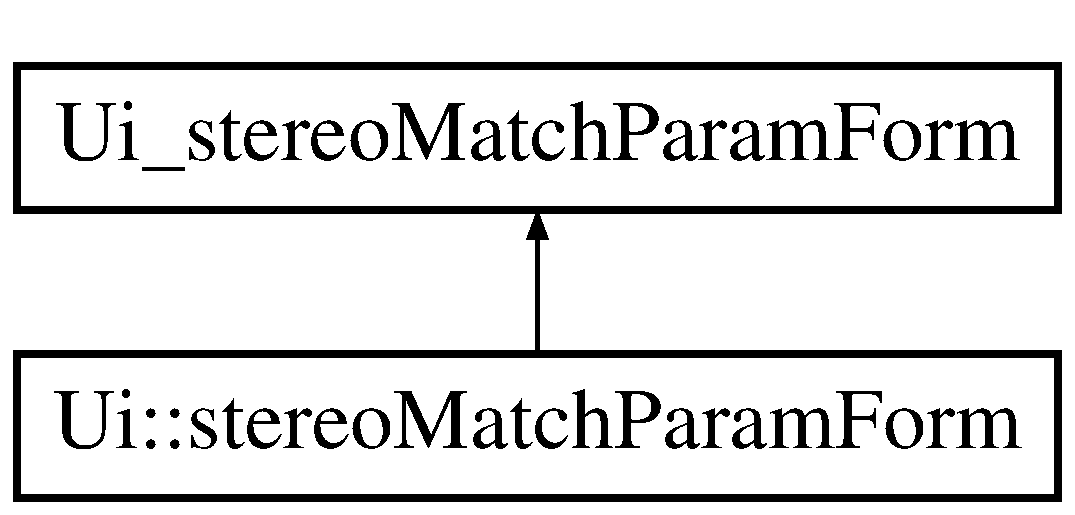
\includegraphics[height=2.000000cm]{class_ui__stereo_match_param_form}
\end{center}
\end{figure}
\subsection*{Public Member Functions}
\begin{DoxyCompactItemize}
\item 
\hypertarget{class_ui__stereo_match_param_form_a2ee193c41bb8dc1a1d1d29ea1e630738}{}void {\bfseries setup\+Ui} (Q\+Widget $\ast$\hyperlink{classstereo_match_param_form}{stereo\+Match\+Param\+Form})\label{class_ui__stereo_match_param_form_a2ee193c41bb8dc1a1d1d29ea1e630738}

\item 
\hypertarget{class_ui__stereo_match_param_form_a6fbd6635b0b75c5016172e0aaa5118aa}{}void {\bfseries retranslate\+Ui} (Q\+Widget $\ast$\hyperlink{classstereo_match_param_form}{stereo\+Match\+Param\+Form})\label{class_ui__stereo_match_param_form_a6fbd6635b0b75c5016172e0aaa5118aa}

\end{DoxyCompactItemize}
\subsection*{Public Attributes}
\begin{DoxyCompactItemize}
\item 
\hypertarget{class_ui__stereo_match_param_form_abb8d877f5c25247fdea7f36c9af2f8d2}{}Q\+Tab\+Widget $\ast$ {\bfseries tab\+Widget}\label{class_ui__stereo_match_param_form_abb8d877f5c25247fdea7f36c9af2f8d2}

\item 
\hypertarget{class_ui__stereo_match_param_form_a81fa3bdc0b6ca9761fd62743b0cb0c30}{}Q\+Widget $\ast$ {\bfseries tab\+\_\+2}\label{class_ui__stereo_match_param_form_a81fa3bdc0b6ca9761fd62743b0cb0c30}

\item 
\hypertarget{class_ui__stereo_match_param_form_a69e2547c3fd96e2c7ee9aa1cd8c706a5}{}Q\+Widget $\ast$ {\bfseries layout\+Widget\+\_\+2}\label{class_ui__stereo_match_param_form_a69e2547c3fd96e2c7ee9aa1cd8c706a5}

\item 
\hypertarget{class_ui__stereo_match_param_form_a84a88e23bf803afdecff5bbc7a78c100}{}Q\+Grid\+Layout $\ast$ {\bfseries grid\+Layout\+\_\+12}\label{class_ui__stereo_match_param_form_a84a88e23bf803afdecff5bbc7a78c100}

\item 
\hypertarget{class_ui__stereo_match_param_form_a6970e88ed6d533df2245580de310e50e}{}Q\+Grid\+Layout $\ast$ {\bfseries grid\+Layout\+\_\+18}\label{class_ui__stereo_match_param_form_a6970e88ed6d533df2245580de310e50e}

\item 
\hypertarget{class_ui__stereo_match_param_form_a680c1868cec7f53a9e80ff1b83054131}{}Q\+Label $\ast$ {\bfseries label\+\_\+16}\label{class_ui__stereo_match_param_form_a680c1868cec7f53a9e80ff1b83054131}

\item 
\hypertarget{class_ui__stereo_match_param_form_ab0163a23078a9643ec70a1a3b9de9d5f}{}Q\+Slider $\ast$ {\bfseries horizontal\+Slider\+\_\+sgbm\+\_\+uniqueness\+\_\+ratio}\label{class_ui__stereo_match_param_form_ab0163a23078a9643ec70a1a3b9de9d5f}

\item 
\hypertarget{class_ui__stereo_match_param_form_aa30957c62389918bf50f44fb44345198}{}Q\+Label $\ast$ {\bfseries label\+\_\+sgbm\+\_\+uniqueness\+\_\+ratio}\label{class_ui__stereo_match_param_form_aa30957c62389918bf50f44fb44345198}

\item 
\hypertarget{class_ui__stereo_match_param_form_a034035cb925a630f635021aa1e8e62e5}{}Q\+Grid\+Layout $\ast$ {\bfseries grid\+Layout\+\_\+19}\label{class_ui__stereo_match_param_form_a034035cb925a630f635021aa1e8e62e5}

\item 
\hypertarget{class_ui__stereo_match_param_form_aae8a30fe4ca18330a3288af865c90b66}{}Q\+Label $\ast$ {\bfseries label\+\_\+17}\label{class_ui__stereo_match_param_form_aae8a30fe4ca18330a3288af865c90b66}

\item 
\hypertarget{class_ui__stereo_match_param_form_a7a3d6c75d3aa5959d64931946ef72ece}{}Q\+Slider $\ast$ {\bfseries horizontal\+Slider\+\_\+sgbm\+\_\+speckle\+\_\+window\+\_\+size}\label{class_ui__stereo_match_param_form_a7a3d6c75d3aa5959d64931946ef72ece}

\item 
\hypertarget{class_ui__stereo_match_param_form_a0cc71d793ec70679a77b2c40bbb5d8b3}{}Q\+Label $\ast$ {\bfseries label\+\_\+sgbm\+\_\+speckle\+\_\+window\+\_\+size}\label{class_ui__stereo_match_param_form_a0cc71d793ec70679a77b2c40bbb5d8b3}

\item 
\hypertarget{class_ui__stereo_match_param_form_a350d90dfb49ea1741439502243a7dfc6}{}Q\+Grid\+Layout $\ast$ {\bfseries grid\+Layout\+\_\+20}\label{class_ui__stereo_match_param_form_a350d90dfb49ea1741439502243a7dfc6}

\item 
\hypertarget{class_ui__stereo_match_param_form_a336a5cb093fed5588f5555f55604e199}{}Q\+Label $\ast$ {\bfseries label\+\_\+18}\label{class_ui__stereo_match_param_form_a336a5cb093fed5588f5555f55604e199}

\item 
\hypertarget{class_ui__stereo_match_param_form_ac7dc5ea062016d990b47e67c60106c8a}{}Q\+Slider $\ast$ {\bfseries horizontal\+Slider\+\_\+sgbm\+\_\+speckle\+\_\+range}\label{class_ui__stereo_match_param_form_ac7dc5ea062016d990b47e67c60106c8a}

\item 
\hypertarget{class_ui__stereo_match_param_form_aba6eea3b628358b810caef4e74847f64}{}Q\+Label $\ast$ {\bfseries label\+\_\+sgbm\+\_\+speckle\+\_\+range}\label{class_ui__stereo_match_param_form_aba6eea3b628358b810caef4e74847f64}

\item 
\hypertarget{class_ui__stereo_match_param_form_a190c5e5ece68d55fbd7402c426b8ba35}{}Q\+Grid\+Layout $\ast$ {\bfseries grid\+Layout\+\_\+13}\label{class_ui__stereo_match_param_form_a190c5e5ece68d55fbd7402c426b8ba35}

\item 
\hypertarget{class_ui__stereo_match_param_form_a5815c64635568453493b4d5290c9f581}{}Q\+Label $\ast$ {\bfseries label\+\_\+11}\label{class_ui__stereo_match_param_form_a5815c64635568453493b4d5290c9f581}

\item 
\hypertarget{class_ui__stereo_match_param_form_abebc59cc2661f7662665949913ab41b6}{}Q\+Slider $\ast$ {\bfseries horizontal\+Slider\+\_\+sgbm\+\_\+pre\+\_\+filter\+\_\+cap}\label{class_ui__stereo_match_param_form_abebc59cc2661f7662665949913ab41b6}

\item 
\hypertarget{class_ui__stereo_match_param_form_a9cbccad1275630d69ca8d6dc27bae9ee}{}Q\+Label $\ast$ {\bfseries label\+\_\+sgbm\+\_\+pre\+\_\+filter\+\_\+cap}\label{class_ui__stereo_match_param_form_a9cbccad1275630d69ca8d6dc27bae9ee}

\item 
\hypertarget{class_ui__stereo_match_param_form_aecc31d5429c169a9dda3d63bdab3f8cc}{}Q\+Grid\+Layout $\ast$ {\bfseries grid\+Layout\+\_\+14}\label{class_ui__stereo_match_param_form_aecc31d5429c169a9dda3d63bdab3f8cc}

\item 
\hypertarget{class_ui__stereo_match_param_form_ac86149f27dbbe7b807063d1e42d5a47f}{}Q\+Label $\ast$ {\bfseries label\+\_\+12}\label{class_ui__stereo_match_param_form_ac86149f27dbbe7b807063d1e42d5a47f}

\item 
\hypertarget{class_ui__stereo_match_param_form_a2034270b3a285edbc94519f86ab71e0f}{}Q\+Slider $\ast$ {\bfseries horizontal\+Slider\+\_\+sgbm\+\_\+sad\+\_\+window\+\_\+size}\label{class_ui__stereo_match_param_form_a2034270b3a285edbc94519f86ab71e0f}

\item 
\hypertarget{class_ui__stereo_match_param_form_ab21171704c44df90021e86e5ffc6640f}{}Q\+Label $\ast$ {\bfseries label\+\_\+sgbm\+\_\+sad\+\_\+window\+\_\+size}\label{class_ui__stereo_match_param_form_ab21171704c44df90021e86e5ffc6640f}

\item 
\hypertarget{class_ui__stereo_match_param_form_a1266646083de55945c5ce0383fa26da4}{}Q\+Grid\+Layout $\ast$ {\bfseries grid\+Layout\+\_\+15}\label{class_ui__stereo_match_param_form_a1266646083de55945c5ce0383fa26da4}

\item 
\hypertarget{class_ui__stereo_match_param_form_a6523fa7a282cf47169c95c55ab7ad5f6}{}Q\+Label $\ast$ {\bfseries label\+\_\+13}\label{class_ui__stereo_match_param_form_a6523fa7a282cf47169c95c55ab7ad5f6}

\item 
\hypertarget{class_ui__stereo_match_param_form_a6e4dc6a079d9683a99081c6f76435cdb}{}Q\+Slider $\ast$ {\bfseries horizontal\+Slider\+\_\+sgbm\+\_\+min\+\_\+disp}\label{class_ui__stereo_match_param_form_a6e4dc6a079d9683a99081c6f76435cdb}

\item 
\hypertarget{class_ui__stereo_match_param_form_a68c281ec8c86df87af5cacea5615692d}{}Q\+Label $\ast$ {\bfseries label\+\_\+sgbm\+\_\+min\+\_\+disp}\label{class_ui__stereo_match_param_form_a68c281ec8c86df87af5cacea5615692d}

\item 
\hypertarget{class_ui__stereo_match_param_form_a259143b1b23d4326d004e4ae0b397a38}{}Q\+Grid\+Layout $\ast$ {\bfseries grid\+Layout\+\_\+16}\label{class_ui__stereo_match_param_form_a259143b1b23d4326d004e4ae0b397a38}

\item 
\hypertarget{class_ui__stereo_match_param_form_a43f58321c5b15099097d20e9bc9ccc33}{}Q\+Label $\ast$ {\bfseries label\+\_\+14}\label{class_ui__stereo_match_param_form_a43f58321c5b15099097d20e9bc9ccc33}

\item 
\hypertarget{class_ui__stereo_match_param_form_a1d00320c458213fc3aca20d411d919d5}{}Q\+Slider $\ast$ {\bfseries horizontal\+Slider\+\_\+sgbm\+\_\+num\+\_\+of\+\_\+disp}\label{class_ui__stereo_match_param_form_a1d00320c458213fc3aca20d411d919d5}

\item 
\hypertarget{class_ui__stereo_match_param_form_aefa17e9cfd7c13f9cd309258ffd3285c}{}Q\+Label $\ast$ {\bfseries label\+\_\+sgbm\+\_\+num\+\_\+of\+\_\+disp}\label{class_ui__stereo_match_param_form_aefa17e9cfd7c13f9cd309258ffd3285c}

\item 
\hypertarget{class_ui__stereo_match_param_form_adeb716a72003db1c76d626d46b3cdeec}{}Q\+Widget $\ast$ {\bfseries tab}\label{class_ui__stereo_match_param_form_adeb716a72003db1c76d626d46b3cdeec}

\item 
\hypertarget{class_ui__stereo_match_param_form_aed1473a88a5a5319d988ced9499151c1}{}Q\+Widget $\ast$ {\bfseries layout\+Widget}\label{class_ui__stereo_match_param_form_aed1473a88a5a5319d988ced9499151c1}

\item 
\hypertarget{class_ui__stereo_match_param_form_a673b087be306990110f56e83963ff058}{}Q\+Grid\+Layout $\ast$ {\bfseries grid\+Layout\+\_\+11}\label{class_ui__stereo_match_param_form_a673b087be306990110f56e83963ff058}

\item 
\hypertarget{class_ui__stereo_match_param_form_a8452afd4c52b464d5ed7cdb4e44e6998}{}Q\+Grid\+Layout $\ast$ {\bfseries grid\+Layout}\label{class_ui__stereo_match_param_form_a8452afd4c52b464d5ed7cdb4e44e6998}

\item 
\hypertarget{class_ui__stereo_match_param_form_a5806afaf8e653668090d45861e17f588}{}Q\+Label $\ast$ {\bfseries label}\label{class_ui__stereo_match_param_form_a5806afaf8e653668090d45861e17f588}

\item 
\hypertarget{class_ui__stereo_match_param_form_a8329f439001e88a6688bc2d7a8b39343}{}Q\+Label $\ast$ {\bfseries label\+\_\+bm\+\_\+pre\+\_\+filter\+\_\+size}\label{class_ui__stereo_match_param_form_a8329f439001e88a6688bc2d7a8b39343}

\item 
\hypertarget{class_ui__stereo_match_param_form_a587a5f93cd6e4de4da3e8d0d191b2d1d}{}Q\+Slider $\ast$ {\bfseries horizontal\+Slider\+\_\+bm\+\_\+pre\+\_\+filter\+\_\+size}\label{class_ui__stereo_match_param_form_a587a5f93cd6e4de4da3e8d0d191b2d1d}

\item 
\hypertarget{class_ui__stereo_match_param_form_a2658fceb42fc0c4a923fc97d3e5e4022}{}Q\+Grid\+Layout $\ast$ {\bfseries grid\+Layout\+\_\+2}\label{class_ui__stereo_match_param_form_a2658fceb42fc0c4a923fc97d3e5e4022}

\item 
\hypertarget{class_ui__stereo_match_param_form_a6572935fd423dc1a6bd7596d63e2a832}{}Q\+Label $\ast$ {\bfseries label\+\_\+2}\label{class_ui__stereo_match_param_form_a6572935fd423dc1a6bd7596d63e2a832}

\item 
\hypertarget{class_ui__stereo_match_param_form_af0e2b3488e0516b0ae49764e799fa0c4}{}Q\+Slider $\ast$ {\bfseries horizontal\+Slider\+\_\+bm\+\_\+pre\+\_\+filter\+\_\+cap}\label{class_ui__stereo_match_param_form_af0e2b3488e0516b0ae49764e799fa0c4}

\item 
\hypertarget{class_ui__stereo_match_param_form_a65529ef56665495a3207afad4027da91}{}Q\+Label $\ast$ {\bfseries label\+\_\+bm\+\_\+pre\+\_\+filter\+\_\+cap}\label{class_ui__stereo_match_param_form_a65529ef56665495a3207afad4027da91}

\item 
\hypertarget{class_ui__stereo_match_param_form_ad1e1edd9fdae71ec506c07150f73e912}{}Q\+Grid\+Layout $\ast$ {\bfseries grid\+Layout\+\_\+4}\label{class_ui__stereo_match_param_form_ad1e1edd9fdae71ec506c07150f73e912}

\item 
\hypertarget{class_ui__stereo_match_param_form_a8f2edaf8593aa6a83f2cc2b592081260}{}Q\+Label $\ast$ {\bfseries label\+\_\+3}\label{class_ui__stereo_match_param_form_a8f2edaf8593aa6a83f2cc2b592081260}

\item 
\hypertarget{class_ui__stereo_match_param_form_a796cb93970db2c414493dfb990dc6086}{}Q\+Slider $\ast$ {\bfseries horizontal\+Slider\+\_\+bm\+\_\+sad\+\_\+window\+\_\+size}\label{class_ui__stereo_match_param_form_a796cb93970db2c414493dfb990dc6086}

\item 
\hypertarget{class_ui__stereo_match_param_form_afed878e1cac18b7c82e9b5cf385c1802}{}Q\+Label $\ast$ {\bfseries label\+\_\+bm\+\_\+sad\+\_\+window\+\_\+size}\label{class_ui__stereo_match_param_form_afed878e1cac18b7c82e9b5cf385c1802}

\item 
\hypertarget{class_ui__stereo_match_param_form_a7a087c7b29cd298f7651e90278235164}{}Q\+Grid\+Layout $\ast$ {\bfseries grid\+Layout\+\_\+5}\label{class_ui__stereo_match_param_form_a7a087c7b29cd298f7651e90278235164}

\item 
\hypertarget{class_ui__stereo_match_param_form_a70b7ee5a8bb2bbe63e80a57222a71595}{}Q\+Label $\ast$ {\bfseries label\+\_\+4}\label{class_ui__stereo_match_param_form_a70b7ee5a8bb2bbe63e80a57222a71595}

\item 
\hypertarget{class_ui__stereo_match_param_form_ab6277ce55fa38ab6a7089fb1949356ff}{}Q\+Slider $\ast$ {\bfseries horizontal\+Slider\+\_\+bm\+\_\+min\+\_\+disp}\label{class_ui__stereo_match_param_form_ab6277ce55fa38ab6a7089fb1949356ff}

\item 
\hypertarget{class_ui__stereo_match_param_form_a6f61a5b917bc2507230e5c3836a65be2}{}Q\+Label $\ast$ {\bfseries label\+\_\+bm\+\_\+min\+\_\+disp}\label{class_ui__stereo_match_param_form_a6f61a5b917bc2507230e5c3836a65be2}

\item 
\hypertarget{class_ui__stereo_match_param_form_a940af64b09ed60215718d7501d700999}{}Q\+Grid\+Layout $\ast$ {\bfseries grid\+Layout\+\_\+6}\label{class_ui__stereo_match_param_form_a940af64b09ed60215718d7501d700999}

\item 
\hypertarget{class_ui__stereo_match_param_form_af96cde3df18f7d9d9e0cef8a33e65529}{}Q\+Label $\ast$ {\bfseries label\+\_\+8}\label{class_ui__stereo_match_param_form_af96cde3df18f7d9d9e0cef8a33e65529}

\item 
\hypertarget{class_ui__stereo_match_param_form_a70bb71d924ceadf9a62718c287df76a2}{}Q\+Slider $\ast$ {\bfseries horizontal\+Slider\+\_\+bm\+\_\+num\+\_\+of\+\_\+disp}\label{class_ui__stereo_match_param_form_a70bb71d924ceadf9a62718c287df76a2}

\item 
\hypertarget{class_ui__stereo_match_param_form_a71fe94fd40b480223b2c72df998386dd}{}Q\+Label $\ast$ {\bfseries label\+\_\+bm\+\_\+num\+\_\+of\+\_\+disp}\label{class_ui__stereo_match_param_form_a71fe94fd40b480223b2c72df998386dd}

\item 
\hypertarget{class_ui__stereo_match_param_form_a666e5c548a04ca8d733282522ccf972b}{}Q\+Grid\+Layout $\ast$ {\bfseries grid\+Layout\+\_\+7}\label{class_ui__stereo_match_param_form_a666e5c548a04ca8d733282522ccf972b}

\item 
\hypertarget{class_ui__stereo_match_param_form_ae3bad7c4b99ccf7f128b37c616ccb002}{}Q\+Label $\ast$ {\bfseries label\+\_\+6}\label{class_ui__stereo_match_param_form_ae3bad7c4b99ccf7f128b37c616ccb002}

\item 
\hypertarget{class_ui__stereo_match_param_form_abb509d739bf22f4314cb758321fc98a6}{}Q\+Slider $\ast$ {\bfseries horizontal\+Slider\+\_\+bm\+\_\+texture\+\_\+thresh}\label{class_ui__stereo_match_param_form_abb509d739bf22f4314cb758321fc98a6}

\item 
\hypertarget{class_ui__stereo_match_param_form_ac2f87d9ef16caac9de2c9300deba0cee}{}Q\+Label $\ast$ {\bfseries label\+\_\+bm\+\_\+texture\+\_\+thresh}\label{class_ui__stereo_match_param_form_ac2f87d9ef16caac9de2c9300deba0cee}

\item 
\hypertarget{class_ui__stereo_match_param_form_a25addba2697915df9f5c13652977b308}{}Q\+Grid\+Layout $\ast$ {\bfseries grid\+Layout\+\_\+10}\label{class_ui__stereo_match_param_form_a25addba2697915df9f5c13652977b308}

\item 
\hypertarget{class_ui__stereo_match_param_form_afe948e4a12e88c5e42761f7f41abfd75}{}Q\+Label $\ast$ {\bfseries label\+\_\+7}\label{class_ui__stereo_match_param_form_afe948e4a12e88c5e42761f7f41abfd75}

\item 
\hypertarget{class_ui__stereo_match_param_form_ad0410d69d8e62e909c14513610f40562}{}Q\+Slider $\ast$ {\bfseries horizontal\+Slider\+\_\+bm\+\_\+uniqueness\+\_\+ratio}\label{class_ui__stereo_match_param_form_ad0410d69d8e62e909c14513610f40562}

\item 
\hypertarget{class_ui__stereo_match_param_form_a878dd579dea03d6ce1c69707a4ee1c44}{}Q\+Label $\ast$ {\bfseries label\+\_\+bm\+\_\+uniqueness\+\_\+ratio}\label{class_ui__stereo_match_param_form_a878dd579dea03d6ce1c69707a4ee1c44}

\item 
\hypertarget{class_ui__stereo_match_param_form_a0d3345c5c49057b521e7ba78a2422455}{}Q\+Grid\+Layout $\ast$ {\bfseries grid\+Layout\+\_\+9}\label{class_ui__stereo_match_param_form_a0d3345c5c49057b521e7ba78a2422455}

\item 
\hypertarget{class_ui__stereo_match_param_form_a904db566b073735699e180a8b9ac6cf3}{}Q\+Label $\ast$ {\bfseries label\+\_\+5}\label{class_ui__stereo_match_param_form_a904db566b073735699e180a8b9ac6cf3}

\item 
\hypertarget{class_ui__stereo_match_param_form_a2712b916c40c02cb3d5dac0f8b635374}{}Q\+Slider $\ast$ {\bfseries horizontal\+Slider\+\_\+bm\+\_\+speckle\+\_\+window\+\_\+size}\label{class_ui__stereo_match_param_form_a2712b916c40c02cb3d5dac0f8b635374}

\item 
\hypertarget{class_ui__stereo_match_param_form_a3f037e43c72f95327ed1594678343eec}{}Q\+Label $\ast$ {\bfseries label\+\_\+bm\+\_\+speckle\+\_\+window\+\_\+size}\label{class_ui__stereo_match_param_form_a3f037e43c72f95327ed1594678343eec}

\item 
\hypertarget{class_ui__stereo_match_param_form_a958e43f0bd113df2ef98cdd4e90f463f}{}Q\+Grid\+Layout $\ast$ {\bfseries grid\+Layout\+\_\+8}\label{class_ui__stereo_match_param_form_a958e43f0bd113df2ef98cdd4e90f463f}

\item 
\hypertarget{class_ui__stereo_match_param_form_ab927e07729e6abaae861aacb9ffa3e25}{}Q\+Label $\ast$ {\bfseries label\+\_\+9}\label{class_ui__stereo_match_param_form_ab927e07729e6abaae861aacb9ffa3e25}

\item 
\hypertarget{class_ui__stereo_match_param_form_aaeb747da528e94b0661f720480a3f784}{}Q\+Slider $\ast$ {\bfseries horizontal\+Slider\+\_\+bm\+\_\+speckle\+\_\+range}\label{class_ui__stereo_match_param_form_aaeb747da528e94b0661f720480a3f784}

\item 
\hypertarget{class_ui__stereo_match_param_form_a7e6e4dd880bd0797b26a721853b35425}{}Q\+Label $\ast$ {\bfseries label\+\_\+bm\+\_\+speckle\+\_\+range}\label{class_ui__stereo_match_param_form_a7e6e4dd880bd0797b26a721853b35425}

\end{DoxyCompactItemize}


The documentation for this class was generated from the following file\+:\begin{DoxyCompactItemize}
\item 
D\+:/\+Qt\+Program/\+Qt5/\+Fusion/ui\+\_\+stereomatchparamform.\+h\end{DoxyCompactItemize}

\hypertarget{struct_sensor_info_1_1vehicle_info}{}\section{Sensor\+Info\+:\+:vehicle\+Info Struct Reference}
\label{struct_sensor_info_1_1vehicle_info}\index{Sensor\+Info\+::vehicle\+Info@{Sensor\+Info\+::vehicle\+Info}}


The \hyperlink{struct_sensor_info_1_1vehicle_info}{vehicle\+Info} struct to save the vehicle\textquotesingle{}s basic info.  


\subsection*{Public Attributes}
\begin{DoxyCompactItemize}
\item 
\hypertarget{struct_sensor_info_1_1vehicle_info_a67374d3ae7011f29a00f8d4ca2266e8a}{}cv\+::\+Point \hyperlink{struct_sensor_info_1_1vehicle_info_a67374d3ae7011f29a00f8d4ca2266e8a}{V\+C\+P}\label{struct_sensor_info_1_1vehicle_info_a67374d3ae7011f29a00f8d4ca2266e8a}

\begin{DoxyCompactList}\small\item\em fused topview vehicle current position (pixel) \end{DoxyCompactList}\item 
\hypertarget{struct_sensor_info_1_1vehicle_info_ac7321d39414cbd87c3408bae40f2cbc2}{}double \hyperlink{struct_sensor_info_1_1vehicle_info_ac7321d39414cbd87c3408bae40f2cbc2}{width}\label{struct_sensor_info_1_1vehicle_info_ac7321d39414cbd87c3408bae40f2cbc2}

\begin{DoxyCompactList}\small\item\em average vehicle\textquotesingle{}s size (cm) \end{DoxyCompactList}\item 
\hypertarget{struct_sensor_info_1_1vehicle_info_af0cad1e9f4e477f8226a980e8809a592}{}double \hyperlink{struct_sensor_info_1_1vehicle_info_af0cad1e9f4e477f8226a980e8809a592}{length}\label{struct_sensor_info_1_1vehicle_info_af0cad1e9f4e477f8226a980e8809a592}

\begin{DoxyCompactList}\small\item\em (cm) \end{DoxyCompactList}\item 
\hypertarget{struct_sensor_info_1_1vehicle_info_a0087921d189f7eb79b2cf980fb4c1e9d}{}int \hyperlink{struct_sensor_info_1_1vehicle_info_a0087921d189f7eb79b2cf980fb4c1e9d}{width\+\_\+pixel}\label{struct_sensor_info_1_1vehicle_info_a0087921d189f7eb79b2cf980fb4c1e9d}

\begin{DoxyCompactList}\small\item\em (pixel) \end{DoxyCompactList}\item 
\hypertarget{struct_sensor_info_1_1vehicle_info_ae2e64b364b8d0b2fa1f675001d60227a}{}int \hyperlink{struct_sensor_info_1_1vehicle_info_ae2e64b364b8d0b2fa1f675001d60227a}{length\+\_\+pixel}\label{struct_sensor_info_1_1vehicle_info_ae2e64b364b8d0b2fa1f675001d60227a}

\begin{DoxyCompactList}\small\item\em (pixel) \end{DoxyCompactList}\item 
\hypertarget{struct_sensor_info_1_1vehicle_info_a8085fa111d0de5dadee99f4d4ff3dc3c}{}double \hyperlink{struct_sensor_info_1_1vehicle_info_a8085fa111d0de5dadee99f4d4ff3dc3c}{head\+\_\+pos}\label{struct_sensor_info_1_1vehicle_info_a8085fa111d0de5dadee99f4d4ff3dc3c}

\begin{DoxyCompactList}\small\item\em (cm) \end{DoxyCompactList}\item 
\hypertarget{struct_sensor_info_1_1vehicle_info_ab4de8e0f9f6b454fb85740c240092363}{}int \hyperlink{struct_sensor_info_1_1vehicle_info_ab4de8e0f9f6b454fb85740c240092363}{head\+\_\+pos\+\_\+pixel}\label{struct_sensor_info_1_1vehicle_info_ab4de8e0f9f6b454fb85740c240092363}

\begin{DoxyCompactList}\small\item\em (pixel) \end{DoxyCompactList}\item 
\hypertarget{struct_sensor_info_1_1vehicle_info_a9b3e432d4b6fc0fd70a36535f4ed4ce0}{}cv\+::\+Rect \hyperlink{struct_sensor_info_1_1vehicle_info_a9b3e432d4b6fc0fd70a36535f4ed4ce0}{rect}\label{struct_sensor_info_1_1vehicle_info_a9b3e432d4b6fc0fd70a36535f4ed4ce0}

\begin{DoxyCompactList}\small\item\em (pixel) \end{DoxyCompactList}\item 
\hypertarget{struct_sensor_info_1_1vehicle_info_a42bb5037d3a9b07ecec7ad288763856c}{}cv\+::\+Scalar \hyperlink{struct_sensor_info_1_1vehicle_info_a42bb5037d3a9b07ecec7ad288763856c}{color}\label{struct_sensor_info_1_1vehicle_info_a42bb5037d3a9b07ecec7ad288763856c}

\begin{DoxyCompactList}\small\item\em vehicle color on fused tovpiew \end{DoxyCompactList}\end{DoxyCompactItemize}


\subsection{Detailed Description}
The \hyperlink{struct_sensor_info_1_1vehicle_info}{vehicle\+Info} struct to save the vehicle\textquotesingle{}s basic info. 

The documentation for this struct was generated from the following file\+:\begin{DoxyCompactItemize}
\item 
D\+:/\+Qt\+Program/\+Qt5/\+Fusion/sensorinfo.\+h\end{DoxyCompactItemize}

\hypertarget{struct_v_e_l___e_s_t_i}{}\section{V\+E\+L\+\_\+\+E\+S\+T\+I Struct Reference}
\label{struct_v_e_l___e_s_t_i}\index{V\+E\+L\+\_\+\+E\+S\+T\+I@{V\+E\+L\+\_\+\+E\+S\+T\+I}}
\subsection*{Public Types}
\begin{DoxyCompactItemize}
\item 
\hypertarget{struct_v_e_l___e_s_t_i_a46e0fedd788029c2a68abc7ec2010b17}{}enum \{ \\*
{\bfseries M\+\_\+\+P\+E\+R\+\_\+\+F\+R\+A\+M\+E2\+M\+\_\+\+P\+E\+R\+\_\+\+S\+E\+C}, 
{\bfseries M\+\_\+\+P\+E\+R\+\_\+\+F\+R\+A\+M\+E2\+K\+M\+\_\+\+P\+E\+R\+\_\+\+H\+R}, 
{\bfseries C\+M\+\_\+\+P\+E\+R\+\_\+\+F\+R\+A\+M\+E2\+C\+M\+\_\+\+P\+E\+R\+\_\+\+S\+E\+C}, 
{\bfseries C\+M\+\_\+\+P\+E\+R\+\_\+\+F\+R\+A\+M\+E2\+M\+\_\+\+P\+E\+R\+\_\+\+S\+E\+C}, 
\\*
{\bfseries C\+M\+\_\+\+P\+E\+R\+\_\+\+F\+R\+A\+M\+E2\+K\+M\+\_\+\+P\+E\+R\+\_\+\+H\+R}
 \}\label{struct_v_e_l___e_s_t_i_a46e0fedd788029c2a68abc7ec2010b17}

\end{DoxyCompactItemize}


The documentation for this struct was generated from the following file\+:\begin{DoxyCompactItemize}
\item 
D\+:/\+Qt\+Program/\+Qt5/\+Fusion/sensorbase.\+h\end{DoxyCompactItemize}

\hypertarget{struct_v_e_l___u_n_i_t}{}\section{V\+E\+L\+\_\+\+U\+N\+I\+T Struct Reference}
\label{struct_v_e_l___u_n_i_t}\index{V\+E\+L\+\_\+\+U\+N\+I\+T@{V\+E\+L\+\_\+\+U\+N\+I\+T}}
\subsection*{Public Types}
\begin{DoxyCompactItemize}
\item 
\hypertarget{struct_v_e_l___u_n_i_t_a112b0af37f7da59c85ba1ce87d1f4b9d}{}enum \{ {\bfseries M\+\_\+\+P\+E\+R\+\_\+\+S\+E\+C2\+K\+M\+\_\+\+P\+E\+R\+\_\+\+H\+R}, 
{\bfseries C\+M\+\_\+\+P\+E\+R\+\_\+\+S\+E\+C2\+K\+M\+\_\+\+P\+E\+R\+\_\+\+H\+R}, 
{\bfseries K\+M\+\_\+\+P\+E\+R\+\_\+\+H\+R2\+M\+\_\+\+P\+R\+E\+\_\+\+S\+E\+C}, 
{\bfseries K\+M\+\_\+\+P\+E\+R\+\_\+\+H\+R2\+C\+M\+\_\+\+P\+E\+R\+\_\+\+S\+E\+C}
 \}\label{struct_v_e_l___u_n_i_t_a112b0af37f7da59c85ba1ce87d1f4b9d}

\end{DoxyCompactItemize}


The documentation for this struct was generated from the following file\+:\begin{DoxyCompactItemize}
\item 
D\+:/\+Qt\+Program/\+Qt5/\+Fusion/sensorbase.\+h\end{DoxyCompactItemize}

%--- End generated contents ---

% Index
\backmatter
\newpage
\phantomsection
\clearemptydoublepage
\addcontentsline{toc}{chapter}{Index}
\printindex

\end{document}
